\documentclass[]{book}
\usepackage{lmodern}
\usepackage{amssymb,amsmath}
\usepackage{ifxetex,ifluatex}
\usepackage{fixltx2e} % provides \textsubscript
\ifnum 0\ifxetex 1\fi\ifluatex 1\fi=0 % if pdftex
  \usepackage[T1]{fontenc}
  \usepackage[utf8]{inputenc}
\else % if luatex or xelatex
  \ifxetex
    \usepackage{mathspec}
  \else
    \usepackage{fontspec}
  \fi
  \defaultfontfeatures{Ligatures=TeX,Scale=MatchLowercase}
\fi
% use upquote if available, for straight quotes in verbatim environments
\IfFileExists{upquote.sty}{\usepackage{upquote}}{}
% use microtype if available
\IfFileExists{microtype.sty}{%
\usepackage{microtype}
\UseMicrotypeSet[protrusion]{basicmath} % disable protrusion for tt fonts
}{}
\usepackage[margin=1in]{geometry}
\usepackage{hyperref}
\hypersetup{unicode=true,
            pdftitle={ECON 6120I Topics in Empirical Industrial Organization},
            pdfauthor={Kohei Kawaguchi},
            pdfborder={0 0 0},
            breaklinks=true}
\urlstyle{same}  % don't use monospace font for urls
\usepackage{natbib}
\bibliographystyle{plainnat}
\usepackage{color}
\usepackage{fancyvrb}
\newcommand{\VerbBar}{|}
\newcommand{\VERB}{\Verb[commandchars=\\\{\}]}
\DefineVerbatimEnvironment{Highlighting}{Verbatim}{commandchars=\\\{\}}
% Add ',fontsize=\small' for more characters per line
\usepackage{framed}
\definecolor{shadecolor}{RGB}{248,248,248}
\newenvironment{Shaded}{\begin{snugshade}}{\end{snugshade}}
\newcommand{\KeywordTok}[1]{\textcolor[rgb]{0.13,0.29,0.53}{\textbf{#1}}}
\newcommand{\DataTypeTok}[1]{\textcolor[rgb]{0.13,0.29,0.53}{#1}}
\newcommand{\DecValTok}[1]{\textcolor[rgb]{0.00,0.00,0.81}{#1}}
\newcommand{\BaseNTok}[1]{\textcolor[rgb]{0.00,0.00,0.81}{#1}}
\newcommand{\FloatTok}[1]{\textcolor[rgb]{0.00,0.00,0.81}{#1}}
\newcommand{\ConstantTok}[1]{\textcolor[rgb]{0.00,0.00,0.00}{#1}}
\newcommand{\CharTok}[1]{\textcolor[rgb]{0.31,0.60,0.02}{#1}}
\newcommand{\SpecialCharTok}[1]{\textcolor[rgb]{0.00,0.00,0.00}{#1}}
\newcommand{\StringTok}[1]{\textcolor[rgb]{0.31,0.60,0.02}{#1}}
\newcommand{\VerbatimStringTok}[1]{\textcolor[rgb]{0.31,0.60,0.02}{#1}}
\newcommand{\SpecialStringTok}[1]{\textcolor[rgb]{0.31,0.60,0.02}{#1}}
\newcommand{\ImportTok}[1]{#1}
\newcommand{\CommentTok}[1]{\textcolor[rgb]{0.56,0.35,0.01}{\textit{#1}}}
\newcommand{\DocumentationTok}[1]{\textcolor[rgb]{0.56,0.35,0.01}{\textbf{\textit{#1}}}}
\newcommand{\AnnotationTok}[1]{\textcolor[rgb]{0.56,0.35,0.01}{\textbf{\textit{#1}}}}
\newcommand{\CommentVarTok}[1]{\textcolor[rgb]{0.56,0.35,0.01}{\textbf{\textit{#1}}}}
\newcommand{\OtherTok}[1]{\textcolor[rgb]{0.56,0.35,0.01}{#1}}
\newcommand{\FunctionTok}[1]{\textcolor[rgb]{0.00,0.00,0.00}{#1}}
\newcommand{\VariableTok}[1]{\textcolor[rgb]{0.00,0.00,0.00}{#1}}
\newcommand{\ControlFlowTok}[1]{\textcolor[rgb]{0.13,0.29,0.53}{\textbf{#1}}}
\newcommand{\OperatorTok}[1]{\textcolor[rgb]{0.81,0.36,0.00}{\textbf{#1}}}
\newcommand{\BuiltInTok}[1]{#1}
\newcommand{\ExtensionTok}[1]{#1}
\newcommand{\PreprocessorTok}[1]{\textcolor[rgb]{0.56,0.35,0.01}{\textit{#1}}}
\newcommand{\AttributeTok}[1]{\textcolor[rgb]{0.77,0.63,0.00}{#1}}
\newcommand{\RegionMarkerTok}[1]{#1}
\newcommand{\InformationTok}[1]{\textcolor[rgb]{0.56,0.35,0.01}{\textbf{\textit{#1}}}}
\newcommand{\WarningTok}[1]{\textcolor[rgb]{0.56,0.35,0.01}{\textbf{\textit{#1}}}}
\newcommand{\AlertTok}[1]{\textcolor[rgb]{0.94,0.16,0.16}{#1}}
\newcommand{\ErrorTok}[1]{\textcolor[rgb]{0.64,0.00,0.00}{\textbf{#1}}}
\newcommand{\NormalTok}[1]{#1}
\usepackage{longtable,booktabs}
\usepackage{graphicx,grffile}
\makeatletter
\def\maxwidth{\ifdim\Gin@nat@width>\linewidth\linewidth\else\Gin@nat@width\fi}
\def\maxheight{\ifdim\Gin@nat@height>\textheight\textheight\else\Gin@nat@height\fi}
\makeatother
% Scale images if necessary, so that they will not overflow the page
% margins by default, and it is still possible to overwrite the defaults
% using explicit options in \includegraphics[width, height, ...]{}
\setkeys{Gin}{width=\maxwidth,height=\maxheight,keepaspectratio}
\IfFileExists{parskip.sty}{%
\usepackage{parskip}
}{% else
\setlength{\parindent}{0pt}
\setlength{\parskip}{6pt plus 2pt minus 1pt}
}
\setlength{\emergencystretch}{3em}  % prevent overfull lines
\providecommand{\tightlist}{%
  \setlength{\itemsep}{0pt}\setlength{\parskip}{0pt}}
\setcounter{secnumdepth}{5}
% Redefines (sub)paragraphs to behave more like sections
\ifx\paragraph\undefined\else
\let\oldparagraph\paragraph
\renewcommand{\paragraph}[1]{\oldparagraph{#1}\mbox{}}
\fi
\ifx\subparagraph\undefined\else
\let\oldsubparagraph\subparagraph
\renewcommand{\subparagraph}[1]{\oldsubparagraph{#1}\mbox{}}
\fi

%%% Use protect on footnotes to avoid problems with footnotes in titles
\let\rmarkdownfootnote\footnote%
\def\footnote{\protect\rmarkdownfootnote}

%%% Change title format to be more compact
\usepackage{titling}

% Create subtitle command for use in maketitle
\providecommand{\subtitle}[1]{
  \posttitle{
    \begin{center}\large#1\end{center}
    }
}

\setlength{\droptitle}{-2em}

  \title{ECON 6120I Topics in Empirical Industrial Organization}
    \pretitle{\vspace{\droptitle}\centering\huge}
  \posttitle{\par}
    \author{Kohei Kawaguchi}
    \preauthor{\centering\large\emph}
  \postauthor{\par}
      \predate{\centering\large\emph}
  \postdate{\par}
    \date{Last updated: 2019-03-22}

\usepackage{booktabs}

\begin{document}
\maketitle

{
\setcounter{tocdepth}{1}
\tableofcontents
}
\chapter{Syllabus}\label{syllabus}

\section{Instructor Information}\label{instructor-information}

\begin{itemize}
\tightlist
\item
  Instructor:

  \begin{itemize}
  \tightlist
  \item
    Name: Kohei Kawaguchi.
  \item
    Office: LSK6070, Monday 11:00-12:00.
  \end{itemize}
\item
  All questions related to the class have to be publicly asked on the
  discussion board of canvas rather than being privately asked in
  e-mail. The instructor usually does not reply in the evening,
  weekends, and holidays.
\end{itemize}

\section{General Information}\label{general-information}

\subsection{Class Time}\label{class-time}

\begin{itemize}
\tightlist
\item
  Date: Monday.
\item
  Time: 13:30-17:20.
\item
  Venue: CYTG001.
\end{itemize}

\subsection{Description}\label{description}

\begin{itemize}
\item
  This is a PhD-level course for empirical industrial organization. This
  course covers various econometric methods used in industrial
  organization that is often referred to as the structural estimation
  approach. These methods have been gradually developed since 1980s in
  parallel with the modernization of industrial organization based on
  the game theory and now widely applied in antitrust policy, business
  strategy, and neighboring fields such as labor economics and
  international economics.
\item
  This course presumes a good understanding of PhD-level microeconomics
  and microeconometrics. Participants are expected to understand at
  least UG-level industrial organization. This course requires
  participants to write programs mostly in R and sometimes in C++ to
  implement various econometric methods. In particular, all assignments
  will involve such a non-trivial programming task. Even though the
  understanding of these programming languages is not a prerequisite, a
  sharp learning curve will be required. Some experience in other
  programming languages will help. Audit without a credit is not
  admitted for students.
\end{itemize}

\subsection{Expectation and Goals}\label{expectation-and-goals}

\begin{itemize}
\tightlist
\item
  The goal of this course is to learn and practice econometric methods
  for empirical industrial organization. The lecture covers the
  econometric methods that have been developed between 80s and 00s to
  estimate primitive parameters governing imperfect competition among
  firms, such as production and cost function estimation, demand
  function estimation, merger simulation, entry and exit analysis, and
  dynamic decision models. The lecture also covers various new methods
  to recover model primitives in certain mechanisms such as auction,
  matching, network, and bargaining. The emphasis is put on the former
  group of methods, because they are the basis for other new methods.
  Participants will not only understand the theoretical background of
  the methods but also become able to implement these methods from
  scratches by writing their own programs. I will briefly discuss the
  latter class of new methods through reading recent papers. The
  participants will become able to understand and use these new methods.
\end{itemize}

\section{Required Environment}\label{required-environment}

\begin{itemize}
\tightlist
\item
  Participants should bring their laptop to the class. We have enough
  extension codes for students. The laptop should have sufficient RAM
  (at least \(\ge\) 8GB, \(\ge\) 16GB is recommended) and CPU power (at
  least Core i5 grade, Core i7 grade is recommended). Participants are
  fully responsible for their hardware issues. Operating System can be
  arbitrary. The instructor mainly uses OSX High Siera with iMac (Retina
  5K, 27-inch, Late 2015) and Macbook Pro (Retina, 15-inch, Early 2017).
\item
  Please install the following software by the first lecture. Technical
  issues related to the installment should be resolved by yourself,
  because it depends on your local environment. If you had an error,
  copy and paste the error message on a search engine, and find a
  solution. This solves 99.9\% of the problems.

  \begin{itemize}
  \tightlist
  \item
    R: \url{https://www.r-project.org/}
  \item
    RStudio: \url{https://www.rstudio.com/}
  \item
    LaTeX:

    \begin{itemize}
    \tightlist
    \item
      MixTex \url{https://miktex.org/}
    \item
      TeXLive \url{https://www.tug.org/texlive/}
    \item
      MacTeX \url{http://www.tug.org/mactex/}
    \end{itemize}
  \end{itemize}
\end{itemize}

\section{Evaluation}\label{evaluation}

\begin{itemize}
\tightlist
\item
  Assignments (80): In total 8 homework are assigned. Each homework
  involves the implementation of the methods covered in the class. Each
  homework has 10 points. The working hour for each homework will be
  around 10-20 hours.
\item
  Participation (10): Every time a participant asks a question in the
  class, after the class, during the office hour, or in the canvas. the
  participant gets one point, up to 10 points. The participant who asked
  the question writes the name, ID number, his/her question, and my
  answer in a discussion board on the course website to claim a point.
\item
  Referee report (10): Toward the end of the semester, a paper in
  industrial organization is randomly assigned to each participant. Each
  participant writes a critical referee report of the assigned paper in
  A4 2 pages that consists of the summary, contribution, strong and weak
  points of the paper.
\item
  Grading is based on the absolute scores: A+ with more than 80 points,
  A with more than 70 points, A- with more than 60 points, B+ with more
  than 50 points, B with more than 40 points, B- with more than 30
  points and C otherwise.
\end{itemize}

\section{Academic Integrity}\label{academic-integrity}

Without academic integrity, there is no serious learning. Thus you are
expected to hold the highest standard of academic integrity in the
course. You are encouraged to study and do homework in groups. However,
no cheating, plagiarism will be tolerated. Anyone caught cheating,
plagiarism will fail the course. Please make sure adhere to the HKUST
Academic Honor Code at all time (see
\url{http://www.ust.hk/vpaao/integrity/}).

\section{Schedule}\label{schedule}

\begin{itemize}
\tightlist
\item
  Introduction to structural estimation, R and RStudio
\item
  Production function estimation I
\item
  Production function estimation II
\item
  Demand function estimation I
\item
  Demand function estimation II
\item
  Merger Analysis
\item
  Entry and Exit
\item
  Single-Agent Dynamics I
\item
  Single-Agent Dynamics II, I change date due to my business trip
\item
  Dynamic Game I
\item
  Dynamic Game II
\item
  Auction
\item
  Other Mechanisms
\end{itemize}

\section{Course Materials}\label{course-materials}

\subsection{R and RStudio}\label{r-and-rstudio}

\begin{itemize}
\tightlist
\item
  Grolemund, G., 2014, Hands-On Programming with R, O'Reilly.

  \begin{itemize}
  \tightlist
  \item
    Free online version is available:
    \url{https://rstudio-education.github.io/hopr/}.
  \end{itemize}
\item
  Wickham, H., \& Grolemund, G., 2017, R for Data Science, O'Reilly.

  \begin{itemize}
  \tightlist
  \item
    Free online version is available: \url{https://r4ds.had.co.nz/}.
  \end{itemize}
\item
  Boswell, D., \& Foucher, T., 2011, The Art of Readable Code: Simple
  and Practical Techniques for Writing Better Code, O'Reilly.
\end{itemize}

\subsection{Handbook Chapters}\label{handbook-chapters}

\begin{itemize}
\tightlist
\item
  Ackerberg, D., Benkard, C., Berry, S., \& Pakes, A. (2007).
  ``Econometric tools for analyzing market outcomes''. Handbook of
  econometrics, 6, 4171-4276.
\item
  Athey, S., \& Haile, P. A. (2007). ``Nonparametric approaches to
  auctions''. Handbook of Econometrics, 6, 3847-3965.
\item
  Berry, S., \& Reiss, P. (2007). ``Empirical models of entry and market
  structure''. Handbook of Industrial Organization, 3, 1845-1886.
\item
  Bresnahan, T. F. (1989). ``Empirical studies of industries with market
  power''. Handbook of Industrial Organization, 2, 1011-1057.
\item
  Hendricks, K., \& Porter, R. H. (2007). ``An empirical perspective on
  auctions''. Handbook of Industrial Organization, 3, 2073-2143.
\item
  Matzkin, R. L. (2007). ``Nonparametric identification''. Handbook of
  Econometrics, 6, 5307-5368.
\item
  Newey, W. K., \& McFadden, D. (1994). ``Large sample estimation and
  hypothesis testing''. Handbook of Econometrics, 4, 2111-2245.
\item
  Reiss, P. C., \& Wolak, F. A. (2007). ``Structural econometric
  modeling: Rationales and examples from industrial organization''.
  Handbook of Econometrics, 6, 4277-4415.
\end{itemize}

\subsection{Books}\label{books}

\begin{itemize}
\tightlist
\item
  Train, K. E. (2009). Discrete Choice Methods with Simulation,
  Cambridge university press.
\item
  Davis, P., \& Garces, E. (2010). Quantitative Techniques for
  Competition and Antitrust Analysis, Princeton University Press.
\item
  Tirole, J. (1988). The Theory of Industrial Organization, The MIT
  Press.
\end{itemize}

\subsection{Papers}\label{papers}

\begin{itemize}
\tightlist
\item
  The list of important papers are occasionally given during the course.
\end{itemize}

\chapter{Introduction}\label{intro}

\section{Structural Estimation and Counterfactual
Analysis}\label{structural-estimation-and-counterfactual-analysis}

\subsection{Example}\label{example}

\begin{itemize}
\item
  \citet{Igami2017} ``Estimating the Innovator's Dilemma: Structural
  Analysis of Creative Destruction in the Hard Disk Drive Industry,
  1981-1998''.
\item
  \textbf{Question}:
\item
  Does ``Innovator's Dilemma'' \citep{Christensen1997} or the delay of
  innovation among incumbents exist?
\item
  Christensen argued that old winners tend to lag behind entrants even
  when introducing a new technology is not too difficult, with a case
  study of the HDD industry.

  \begin{itemize}
  \tightlist
  \item
    Apple's smartphone vs.~Nokia's feature phones.
  \item
    Amazon vs.~Borders.
  \item
    Kodak's digital camera.
  \end{itemize}
\item
  If it exists, what is the reason for that?
\item
  How do we empirically answer this question?
\end{itemize}

\begin{figure}

{\centering 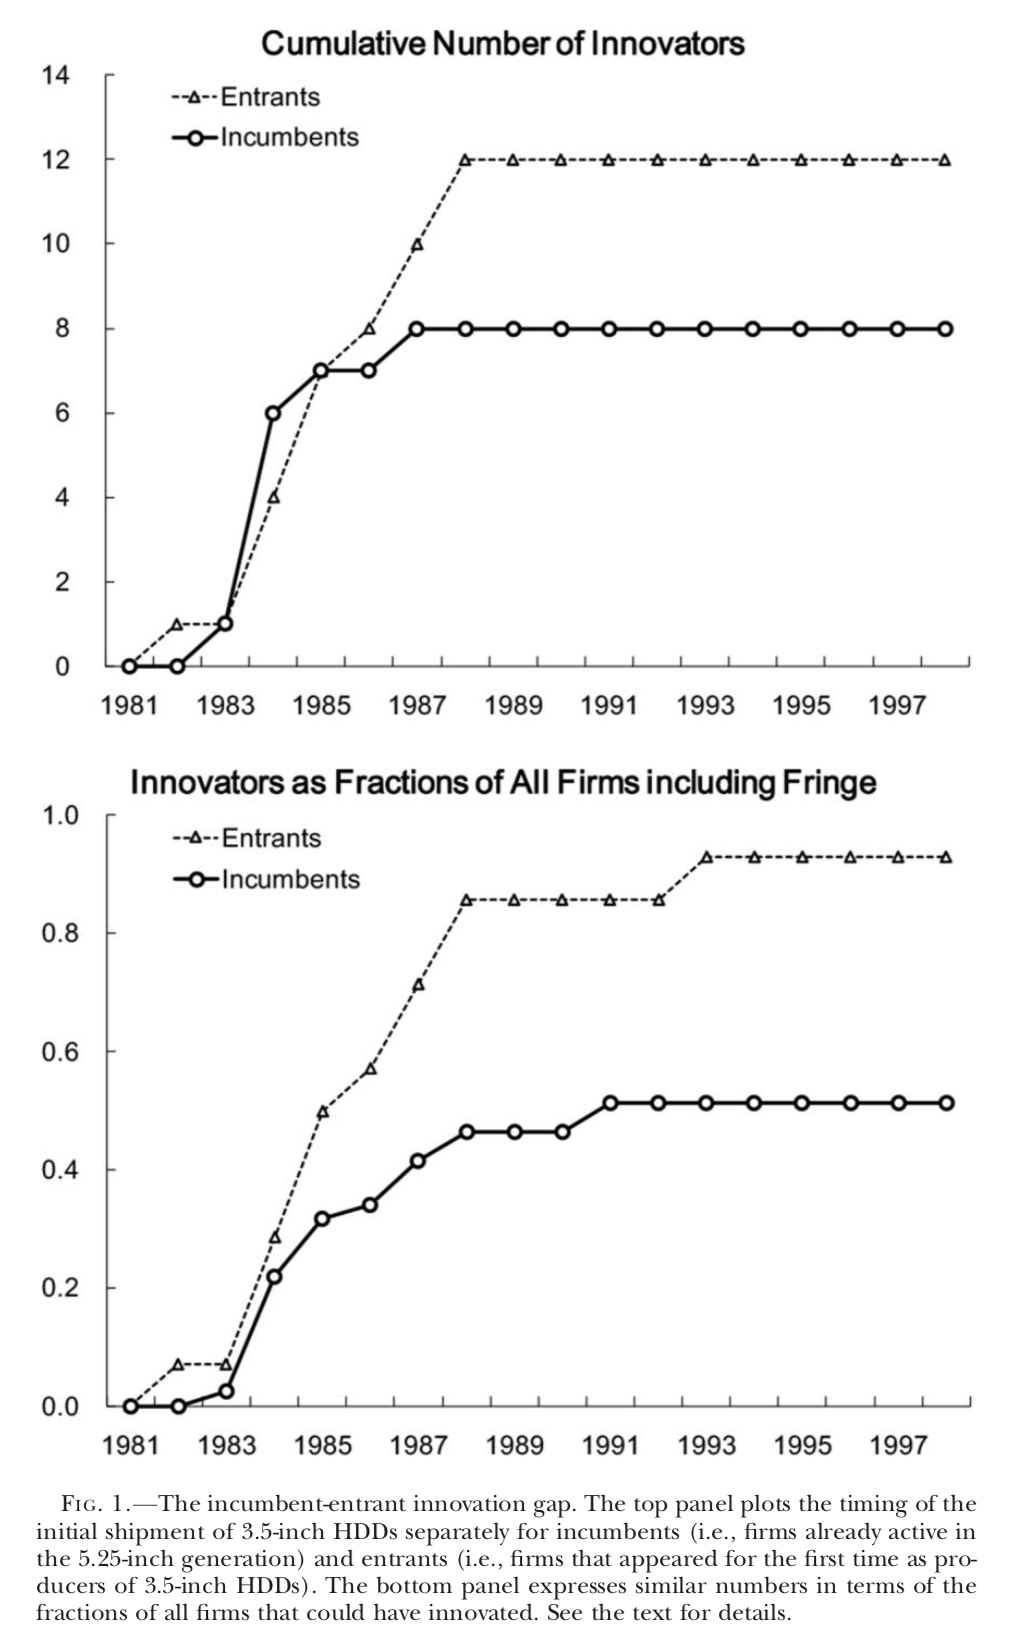
\includegraphics[width=0.8\linewidth]{figuretable/Igam2017Fig1} 

}

\caption{Figure 1 of Igam (2017)}\label{fig:unnamed-chunk-2}
\end{figure}

\begin{itemize}
\item
  \textbf{Hypotheses}:
\item
  Identify potentially competing hypotheses to explain the phenomenon.

  \begin{enumerate}
  \def\labelenumi{\arabic{enumi}.}
  \tightlist
  \item
    Cannibalization: Because of cannibalization, the benefits of
    introducing a new product are smaller for incumbents than for
    entrants.
  \item
    Different costs: The incumbents may have higher costs for innovation
    due to the organizational inertia, but at the same time they may
    have some cost advantage due to accumulated R\&D and better
    financial access.
  \item
    Preemption: The incumbents have additional incentive for innovation
    to preempt potential rivals.
  \item
    Institutional environment: The impacts of the three components
    differ across different institutional contexts such as the rules
    governing patents and market size.
  \end{enumerate}
\item
  Casual empiricists pick up their favorite factors to make up a story.
\item
  Serious empiricists should try to separate the contributions of each
  factor from data.
\item
  To do so, the author develops an economic model that explicitly
  incorporates the above mentioned factors, while keeping the model
  parameters flexible enough to let the data tell the sign and size of
  the effects of each factor on innovation.
\item
  \textbf{Economic model}:
\item
  The time is discrete with finite horizon \(t = 1, \cdots, T\).
\item
  In each year, there is a finite number of firms indexed by \(i\).
\item
  Each firm is in one of the technological states:

  \begin{equation}
  s_{it} \in \{\text{old only, both, new only, potential entrant}\},
  \end{equation}

  where the first two states are for incumbents (stick to the old
  technology or start using the new technology) and the last two states
  are for actual and potential entrants (enter with the new technology
  or stay outside the market).
\item
  In each year:

  \begin{itemize}
  \tightlist
  \item
    Pre-innovation incumbent (\(s_{it} =\) old): exit or innovate by
    paying a sunk cost \(\kappa^{inc}\) (to be \(s_{i, t + 1} =\) both).
  \item
    Post-innovation incumbent (\(s_{it} =\) both): exit or stay to be
    both.
  \item
    Potential entrant (\(s_{it} =\) potential entrant): give up entry or
    enter with the new technology by paying a sunk cost \(\kappa^{net}\)
    (to be \(s_{i, t + 1} =\) new).
  \item
    Actual entrant (\(s_{it} =\) new): exit or stay to be new.
  \end{itemize}
\item
  Given the industry state \(s_t = \{s_{it}\}_i\), the product market
  competition opens and the profit of firm \(i\),
  \(\pi_t(s_{it}, s_{-it})\), is realized for each active firm.
\item
  As the product market competition closes:

  \begin{itemize}
  \tightlist
  \item
    Pre-innovation incumbents draw private cost shocks and make
    decisions: \(a_t^{pre}\).
  \item
    Observing this, post-innovation incumbents draw private cost shocks
    and make decisions: \(a_t^{post}\).
  \item
    Observing this, actual entrants draw private cost shocks and make
    decisions: \(a_t^{act}\).
  \item
    Observing this, potential entrants draw private cost shocks and make
    decisions: \(a_t^{pot}\).
  \end{itemize}
\item
  This is a dynamic game. The equilibrium is defined by the concept of
  \textbf{Markov-perfect equilibrium} \citep{Maskin1988}.
\item
  The representation of the competing theories in the model:

  \begin{itemize}
  \tightlist
  \item
    The existence of cannibalization is represented by the assumption
    that an incumbent maximizes the joint profits of old and new
    technology products.
  \item
    The size of cannibalization is captured by the shape of profit
    function.
  \item
    The difference in the cost of innovation is captured by the
    difference in the sunk costs of innovation.
  \item
    The preemptive incentive for incumbents are embodied in the dynamic
    optimization problem for each incumbent.
  \end{itemize}
\item
  \textbf{Econometric model}:
\item
  The author then turns the economic model into an econometric model.
\item
  This amounts to specify which part of the economic model is
  observed/known and which part is unobserved/unknown.
\item
  The author collects the data set of the HDD industry during 1977-99.
\item
  Based on the data, the author specify the identities of active firms
  and their products and the technologies embodied in the products in
  each year to code their \textbf{state variables}.
\item
  Moreover, by tracking the change in the state, the author code their
  \textbf{action variables}.
\item
  Thus, the state and action variables, \(s_t\) and \(a_t\). These are
  the \textbf{observables}.
\item
  The author does not observe:

  \begin{itemize}
  \tightlist
  \item
    Profit function \(\pi_t(\cdot)\).
  \item
    Sunk cost of innovation for pre-innovation incumbents
    \(\kappa^{inc}\).
  \item
    Sunk cost of entry for potential entrants \(\kappa^{net}\).
  \item
    Private cost shocks.
  \end{itemize}
\item
  These are the \textbf{unobservables}.
\item
  Among the unobservables, the profit function and sunk costs are the
  \textbf{parameter of interets} and the private cost shocks are
  \textbf{nuissance parameters} in the sense only the knowledge about
  the distribution of the latter is demanded.
\item
  \textbf{Identification}:
\item
  Can we infer the unobservables from the observables and the
  restrictions on the distribution of observable by the economic theory?
\item
  The profit function is identified from estimating the demand function
  for each firm's product, and estimating the cost function for each
  firm from using their price setting behavior.
\item
  The sunk costs of innovation are identified from the conditional
  probability of innovation across various states. If the cost is low,
  the probability should be high.
\item
  \textbf{Estimation}:
\item
  The identification established that in principle we can uncover the
  parameters of interests from observables under the restrictions of
  economic theory.
\item
  Finally, we apply a statistical method to the econometric model and
  infer the parameters of interest.
\item
  \textbf{Counterfactual analysis}:
\item
  If we can uncover the parameters of interest, we can conduct
  \textbf{comparative statics}: study the change in the endogenous
  variables when the exogenous variables including the model parameters
  are set different. In the current framework, this exercise is often
  called the \textbf{counterfactual analysis}.
\item
  What if there was no cannibalization?:

  \begin{itemize}
  \tightlist
  \item
    An incumbents separately maximizes the profit from old technology
    and new technology instead of jointly maximizing the profits. Solve
    the model under this new assumption everything else being equal.
  \item
    Free of cannibalization concerns, 8.95 incumbents start producing
    new HDDs in the first 10 years, compared with 6.30 in the baseline.
  \item
    The cumulative numbers of innovators among incumbents and entrants
    differ only by 2.8 compared with 6.45 in the baseline.
  \item
    Thus cannibalization can explain a significant part of the
    incumbent-entrant innovation gap.
  \end{itemize}
\item
  What if there was no preemption?:

  \begin{itemize}
  \tightlist
  \item
    A potential entrant ignores the incumbents' innovations upon making
    entry decisions.
  \item
    Without the preemptive motives, only 6.02 incumbents would innovate
    in the first 10 7ears, compared with 6.30 in the baseline.
  \item
    The cumulative incumbent-entrant innovation gap widen to 8.91
    compared with 6.45 in the baseline.
  \end{itemize}
\item
  The sunk cost of entry is smaller for incumbents than for entrants in
  the baseline.
\item
  \textbf{Interpretations and policy/managerial implication}:
\item
  Despite the cost advantage and the preemptive motives, the speed of
  innovation is slower among incumbents due to the strong
  cannibalization effect.
\item
  Incumbents that attempt to avoid the ``innovator's dilemma'' should
  separate the decision makings between old and new sections inside the
  organization so that it can avoid the concern for cannibalization.
\end{itemize}

\subsection{Recap}\label{recap}

\begin{itemize}
\tightlist
\item
  The structural approach in empirical industrial organization consists
  of the following components:
\end{itemize}

\begin{enumerate}
\def\labelenumi{\arabic{enumi}.}
\tightlist
\item
  Research question.
\item
  Competing hypotheses.
\item
  Economic model.
\item
  Econometric model
\item
  Identification.
\item
  Data collection.
\item
  Data cleaning.
\item
  Estimation.
\item
  Counterfactual analysis.
\item
  Coding.
\item
  Interpretations and policy/managerial implications.
\end{enumerate}

\begin{itemize}
\tightlist
\item
  The goal of this course is to be familiar with the standard
  methodology to complete this process.
\item
  The methodology covered in this class is mostly developed to analyze
  the standard framework to dynamic or oligopoly competition.
\item
  The policy implications are centered around competition policies.
\item
  But the basic idea can be extend to different class of situations such
  as auction, matching, voting, contract, marketing, and so on.
\item
  Note that the depth of the research question and the relevance of the
  policy/managerial implications are the most important part of the
  research.
\item
  Focusing on the methodology in this class is to minimize the time to
  allocate to less important issues and maximize the attention and time
  to the most valuable part in the future research.
\item
  Given a research question, what kind of data is necessary to answer
  the question?
\item
  Given data, what kind of research questions can you address? Which
  question can be credibly answered? Which question can be an
  over-stretch?
\item
  Given a research question and data, what is the best way to answer the
  question? What type of problem can you avoid using the method? What is
  the limitation of your approach? How will you defend the possible
  referee comments?
\item
  Given a result, what kinds of interpretation can you credibly derive?
  What kinds of interpretation can be contested by potential opponents?
  What kinds of contribution can you claim?
\item
  To address these issues is \textbf{necessary} to publish a paper and
  it is \textbf{necessary} to be familiar with the methodology to do so.
\end{itemize}

\subsection{Historical Remark}\label{historical-remark}

\begin{itemize}
\tightlist
\item
  The words \textbf{reduced-form} and \textbf{structural-form} date back
  to the literature of estimation of simultaneous equations in
  macroeconomics \citep{Hsiao1983}.
\item
  Let \(y\) be the vector of observed endogenous variables, \(x\) be the
  vector of observed exogenous variables, and \(\epsilon\) be the vector
  of unobserved exogenous variables.
\item
  The equilibrium condition for \(y\) on \(x\) and \(\epsilon\) is often
  written as:

  \begin{equation}
  Ay + Bx = \Sigma \epsilon. \label{eq:structuralform}
  \end{equation}
\item
  These equations \textbf{implicitly} determine the vector of endogenous
  variables \(y\) .
\item
  If \(A\) is invertible, we can solve the equations for \(y\) to
  obtain:

  \begin{equation}
  y = - A^{-1} B x + A^{-1} \Sigma \epsilon. \label{eq:reducedform}
  \end{equation}
\item
  These equations \textbf{explicitly} determine the vector of endogenous
  variables \(y\).
\item
  Equation \eqref{eq:structuralform} is the \textbf{structural-form} and
  \eqref{eq:reducedform} is the \textbf{reduced-form}.
\item
  If \(y\) and \(x\) are observed and \(x\) is of full column rank, then
  \(A^{-1}B\) and \(A^{-1} \Sigma A^{-1}\) will be estimated by
  regression for \eqref{eq:reducedform}. But this does not mean that
  \(A, B\) and \(\Sigma\) are separately estimated.
\item
  This was the traditional identification problems.
\item
  Thus, reduced-form does not mean either of:

  \begin{itemize}
  \tightlist
  \item
    Regression analysis;
  \item
    Statistical analysis free from economic assumptions.
  \end{itemize}
\item
  Recent development in this line of literature of identification is
  found in \citet{Matzkin2007}.
\item
  In econometrics, the idea of imposing restrictions from economic
  theories seems to have been formalized by the work of
  \citet{Manski1994a} and \citet{Matzkin1994b}.
\end{itemize}

\section{Setting Up The Environment}\label{setting-up-the-environment}

\begin{itemize}
\tightlist
\item
  Assume that R, RStudio and LaTex are all installed in the local
  computer.
\end{itemize}

\subsection{RStudio Project}\label{rstudio-project}

\begin{itemize}
\tightlist
\item
  The assignments should be conducted inside a project folder for this
  course.
\item
  \texttt{File\ \textgreater{}\ New\ Project...\textgreater{}\ New\ Directory\ \textgreater{}\ New\ Directory\ \textgreater{}\ R\ Package\ using\ RcppEigen}.
\item
  Name the directory \texttt{ECON6120I} and place in your favorite
  location.
\item
  You can open this project from the upper right menu of RStudio or by
  double clicking the \texttt{ECON6120I.Rproj} file in the
  \texttt{ECON6120I} directory.
\item
  This navigates you to the root directory of the project.
\item
  In the root directory, make folders named:

  \begin{itemize}
  \tightlist
  \item
    \texttt{assignment}.
  \item
    \texttt{input}.
  \item
    \texttt{output}.
  \item
    \texttt{figuretable}.
  \end{itemize}
\item
  We will store R functions in \texttt{R} folder, C/C++ functions in
  \texttt{src} folder, and data in \texttt{input} folder, data generated
  from the code in \texttt{output}, and figures and tables in
  \texttt{figurtable} folder.
\item
  Open \texttt{src/Makevars} and erase the content. Then, write:
  \texttt{PKG\_CPPFLAGS\ =\ -w\ -std=c++11\ -O3}
\item
  Open \texttt{src/Makevars.win} and erase the content. Then, write:
  \texttt{PKG\_CPPFLAGS\ =\ -w\ -std=c++11}
\end{itemize}

\subsection{Basic Programming in R}\label{basic-programming-in-r}

\begin{itemize}
\tightlist
\item
  \texttt{File\ \textgreater{}\ New\ File\ \textgreater{}\ R\ Script} to
  open \texttt{Untitled} file.
\item
  \texttt{Ctrl\ (Cmd)\ +\ S} to save it with \texttt{test.R} in
  \texttt{assignment} folder.
\item
  In the console, type and push enter:
\end{itemize}

\begin{Shaded}
\begin{Highlighting}[]
\DecValTok{1} \OperatorTok{+}\StringTok{ }\DecValTok{1}
\end{Highlighting}
\end{Shaded}

\begin{verbatim}
## [1] 2
\end{verbatim}

\begin{Shaded}
\begin{Highlighting}[]
\DecValTok{100}\OperatorTok{:}\DecValTok{130}
\end{Highlighting}
\end{Shaded}

\begin{verbatim}
##  [1] 100 101 102 103 104 105 106 107 108 109 110 111 112 113 114 115 116
## [18] 117 118 119 120 121 122 123 124 125 126 127 128 129 130
\end{verbatim}

\begin{itemize}
\tightlist
\item
  This is the interactive way of using R functionalities.
\item
  In \texttt{test.R}, write:
\end{itemize}

\begin{Shaded}
\begin{Highlighting}[]
\DecValTok{1} \OperatorTok{+}\StringTok{ }\DecValTok{1}
\end{Highlighting}
\end{Shaded}

\begin{itemize}
\item
  Then, save the file and push \texttt{Run}.
\item
  Alternatively, place the mouse over the \texttt{1\ +\ 1} line in
  \texttt{test.R} file.
\item
  Then, \texttt{Ctrl\ (Cmd)\ +\ Enter} to run the line.
\item
  In this way, we can write procedures in the file and send to the
  console to run.
\item
  There are functions to conduct basic calculations:
\end{itemize}

\begin{Shaded}
\begin{Highlighting}[]
\DecValTok{1} \OperatorTok{+}\StringTok{ }\DecValTok{2}
\end{Highlighting}
\end{Shaded}

\begin{verbatim}
## [1] 3
\end{verbatim}

\begin{Shaded}
\begin{Highlighting}[]
\DecValTok{2} \OperatorTok{*}\StringTok{ }\DecValTok{3}
\end{Highlighting}
\end{Shaded}

\begin{verbatim}
## [1] 6
\end{verbatim}

\begin{Shaded}
\begin{Highlighting}[]
\DecValTok{4} \OperatorTok{-}\StringTok{ }\DecValTok{1}
\end{Highlighting}
\end{Shaded}

\begin{verbatim}
## [1] 3
\end{verbatim}

\begin{Shaded}
\begin{Highlighting}[]
\DecValTok{6} \OperatorTok{/}\StringTok{ }\DecValTok{2}
\end{Highlighting}
\end{Shaded}

\begin{verbatim}
## [1] 3
\end{verbatim}

\begin{Shaded}
\begin{Highlighting}[]
\DecValTok{2}\OperatorTok{^}\DecValTok{3}
\end{Highlighting}
\end{Shaded}

\begin{verbatim}
## [1] 8
\end{verbatim}

\begin{itemize}
\tightlist
\item
  We can define objects and assign values to them.
\end{itemize}

\begin{Shaded}
\begin{Highlighting}[]
\NormalTok{a <-}\StringTok{ }\DecValTok{1}
\NormalTok{a}
\end{Highlighting}
\end{Shaded}

\begin{verbatim}
## [1] 1
\end{verbatim}

\begin{Shaded}
\begin{Highlighting}[]
\NormalTok{a }\OperatorTok{+}\StringTok{ }\DecValTok{2}
\end{Highlighting}
\end{Shaded}

\begin{verbatim}
## [1] 3
\end{verbatim}

\begin{itemize}
\tightlist
\item
  In addition to scalar object, we can define a vector by:
\end{itemize}

\begin{Shaded}
\begin{Highlighting}[]
\DecValTok{2}\OperatorTok{:}\DecValTok{10}
\end{Highlighting}
\end{Shaded}

\begin{verbatim}
## [1]  2  3  4  5  6  7  8  9 10
\end{verbatim}

\begin{Shaded}
\begin{Highlighting}[]
\DecValTok{3}\OperatorTok{:}\DecValTok{20}
\end{Highlighting}
\end{Shaded}

\begin{verbatim}
##  [1]  3  4  5  6  7  8  9 10 11 12 13 14 15 16 17 18 19 20
\end{verbatim}

\begin{Shaded}
\begin{Highlighting}[]
\KeywordTok{c}\NormalTok{(}\DecValTok{2}\NormalTok{, }\DecValTok{3}\NormalTok{, }\DecValTok{5}\NormalTok{, }\DecValTok{9}\NormalTok{, }\DecValTok{10}\NormalTok{)}
\end{Highlighting}
\end{Shaded}

\begin{verbatim}
## [1]  2  3  5  9 10
\end{verbatim}

\begin{Shaded}
\begin{Highlighting}[]
\KeywordTok{seq}\NormalTok{(}\DecValTok{1}\NormalTok{, }\DecValTok{10}\NormalTok{, }\DecValTok{2}\NormalTok{)}
\end{Highlighting}
\end{Shaded}

\begin{verbatim}
## [1] 1 3 5 7 9
\end{verbatim}

\begin{itemize}
\tightlist
\item
  \texttt{seq} is a function with initial value, end values, and the
  increment value.
\item
  By typing \texttt{seq} in the \texttt{help}, we can read the manual
  page of the function.
\item
  \texttt{seq\ \{base\}} means that this function is named \texttt{seq}
  and is contained in the library called \texttt{base}.
\item
  Some libraries are automatically called when the R is launched, but
  some are not.
\item
  Some libraries are even not installed.
\item
  We can install a library from a repository called \texttt{CRAN}.
\end{itemize}

\begin{Shaded}
\begin{Highlighting}[]
\KeywordTok{install.packages}\NormalTok{(}\StringTok{"ggplot2"}\NormalTok{)}
\end{Highlighting}
\end{Shaded}

\begin{itemize}
\tightlist
\item
  To use the package, we have to load by:
\end{itemize}

\begin{Shaded}
\begin{Highlighting}[]
\KeywordTok{library}\NormalTok{(ggplot2)}
\end{Highlighting}
\end{Shaded}

\begin{itemize}
\tightlist
\item
  Use \texttt{qplot} function in \texttt{ggplot2} library to draw a
  scatter plot.
\end{itemize}

\begin{Shaded}
\begin{Highlighting}[]
\NormalTok{x <-}\StringTok{ }\KeywordTok{c}\NormalTok{(}\OperatorTok{-}\DecValTok{1}\NormalTok{, }\OperatorTok{-}\FloatTok{0.8}\NormalTok{, }\OperatorTok{-}\FloatTok{0.6}\NormalTok{, }\OperatorTok{-}\FloatTok{0.4}\NormalTok{, }\OperatorTok{-}\FloatTok{0.2}\NormalTok{, }\DecValTok{0}\NormalTok{, }\FloatTok{0.2}\NormalTok{, }\FloatTok{0.4}\NormalTok{, }\FloatTok{0.6}\NormalTok{, }\FloatTok{0.7}\NormalTok{, }\DecValTok{1}\NormalTok{)}
\NormalTok{y <-}\StringTok{ }\NormalTok{x}\OperatorTok{^}\DecValTok{3}
\KeywordTok{qplot}\NormalTok{(x, y)}
\end{Highlighting}
\end{Shaded}

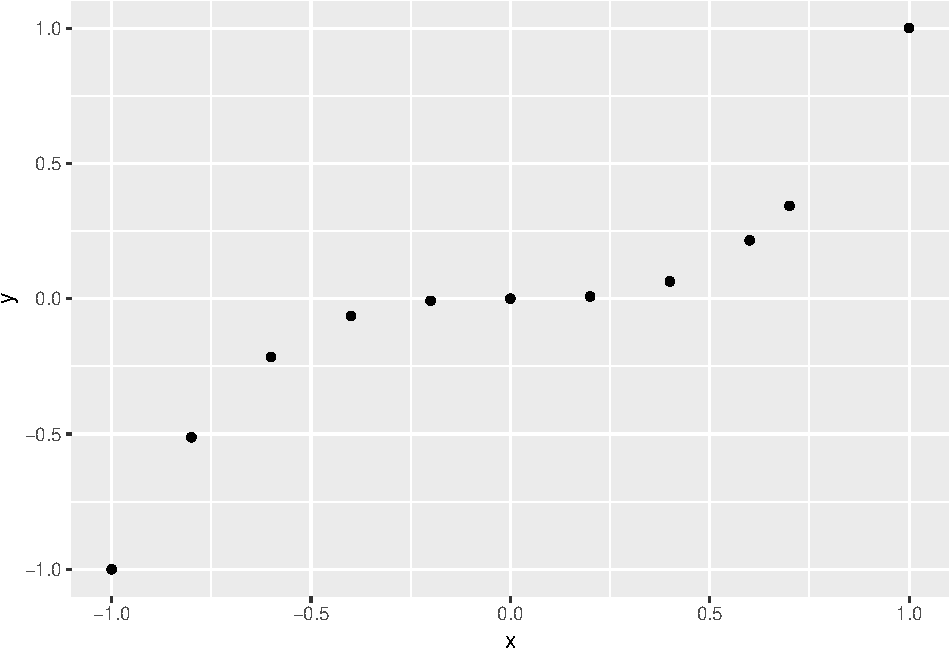
\includegraphics{lecture_files/figure-latex/unnamed-chunk-15-1.pdf} -
Instead of loading a package by \texttt{library}, you can directly call
it as:

\begin{Shaded}
\begin{Highlighting}[]
\NormalTok{ggplot2}\OperatorTok{::}\KeywordTok{qplot}\NormalTok{(x, y)}
\end{Highlighting}
\end{Shaded}

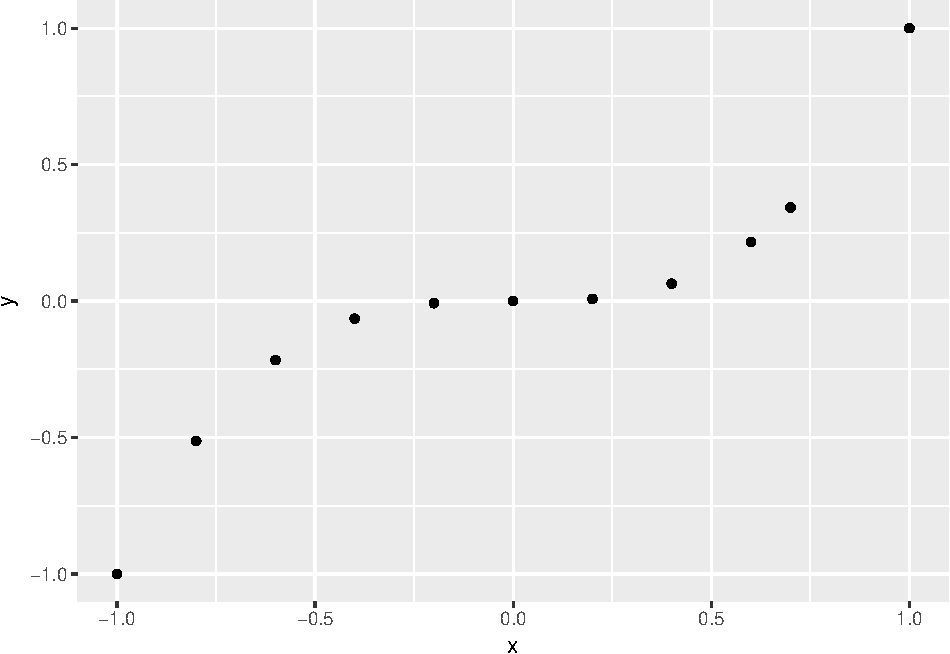
\includegraphics{lecture_files/figure-latex/unnamed-chunk-16-1.pdf}

\begin{itemize}
\tightlist
\item
  We can write own functions.
\end{itemize}

\begin{Shaded}
\begin{Highlighting}[]
\NormalTok{roll <-}\StringTok{ }\ControlFlowTok{function}\NormalTok{(n) \{}
\NormalTok{  die <-}\StringTok{ }\DecValTok{1}\OperatorTok{:}\DecValTok{6}
\NormalTok{  dice <-}\StringTok{ }\KeywordTok{sample}\NormalTok{(die, }\DataTypeTok{size =}\NormalTok{ n, }\DataTypeTok{replace =} \OtherTok{TRUE}\NormalTok{)}
\NormalTok{  y <-}\StringTok{ }\KeywordTok{sum}\NormalTok{(dice)}
  \KeywordTok{return}\NormalTok{(y)}
\NormalTok{\}}
\KeywordTok{roll}\NormalTok{(}\DecValTok{1}\NormalTok{)}
\end{Highlighting}
\end{Shaded}

\begin{verbatim}
## [1] 4
\end{verbatim}

\begin{Shaded}
\begin{Highlighting}[]
\KeywordTok{roll}\NormalTok{(}\DecValTok{2}\NormalTok{)}
\end{Highlighting}
\end{Shaded}

\begin{verbatim}
## [1] 5
\end{verbatim}

\begin{Shaded}
\begin{Highlighting}[]
\KeywordTok{roll}\NormalTok{(}\DecValTok{10}\NormalTok{)}
\end{Highlighting}
\end{Shaded}

\begin{verbatim}
## [1] 42
\end{verbatim}

\begin{Shaded}
\begin{Highlighting}[]
\KeywordTok{roll}\NormalTok{(}\DecValTok{10}\NormalTok{)}
\end{Highlighting}
\end{Shaded}

\begin{verbatim}
## [1] 39
\end{verbatim}

\begin{itemize}
\tightlist
\item
  We can \texttt{set.seed} to obtain the same realization of random
  variables.
\end{itemize}

\begin{Shaded}
\begin{Highlighting}[]
\KeywordTok{set.seed}\NormalTok{(}\DecValTok{1}\NormalTok{)}
\KeywordTok{roll}\NormalTok{(}\DecValTok{10}\NormalTok{)}
\end{Highlighting}
\end{Shaded}

\begin{verbatim}
## [1] 38
\end{verbatim}

\begin{Shaded}
\begin{Highlighting}[]
\KeywordTok{set.seed}\NormalTok{(}\DecValTok{1}\NormalTok{)}
\KeywordTok{roll}\NormalTok{(}\DecValTok{10}\NormalTok{)}
\end{Highlighting}
\end{Shaded}

\begin{verbatim}
## [1] 38
\end{verbatim}

\begin{itemize}
\tightlist
\item
  When a variable used in a function is not given as its argument, the
  function calls the variable in the global environment:
\end{itemize}

\begin{Shaded}
\begin{Highlighting}[]
\NormalTok{y <-}\StringTok{ }\DecValTok{1}
\NormalTok{plus_}\DecValTok{1}\NormalTok{ <-}\StringTok{ }\ControlFlowTok{function}\NormalTok{(x) \{}
  \KeywordTok{return}\NormalTok{(x }\OperatorTok{+}\StringTok{ }\NormalTok{y)}
\NormalTok{\}}
\KeywordTok{plus_1}\NormalTok{(}\DecValTok{1}\NormalTok{)}
\end{Highlighting}
\end{Shaded}

\begin{verbatim}
## [1] 2
\end{verbatim}

\begin{Shaded}
\begin{Highlighting}[]
\KeywordTok{plus_1}\NormalTok{(}\DecValTok{2}\NormalTok{)}
\end{Highlighting}
\end{Shaded}

\begin{verbatim}
## [1] 3
\end{verbatim}

\begin{itemize}
\tightlist
\item
  However, you should NOT do this. All variables used in a function
  should be given as its arguments:
\end{itemize}

\begin{Shaded}
\begin{Highlighting}[]
\NormalTok{y <-}\StringTok{ }\DecValTok{1}
\NormalTok{plus_}\DecValTok{2}\NormalTok{ <-}\StringTok{ }\ControlFlowTok{function}\NormalTok{(x, y) \{}
  \KeywordTok{return}\NormalTok{(x }\OperatorTok{+}\StringTok{ }\NormalTok{y)}
\NormalTok{\}}
\KeywordTok{plus_2}\NormalTok{(}\DecValTok{2}\NormalTok{, }\DecValTok{3}\NormalTok{)}
\end{Highlighting}
\end{Shaded}

\begin{verbatim}
## [1] 5
\end{verbatim}

\begin{Shaded}
\begin{Highlighting}[]
\KeywordTok{plus_2}\NormalTok{(}\DecValTok{2}\NormalTok{, }\DecValTok{4}\NormalTok{)}
\end{Highlighting}
\end{Shaded}

\begin{verbatim}
## [1] 6
\end{verbatim}

\begin{itemize}
\tightlist
\item
  The best practice is to use \texttt{findGlobals} function in
  \texttt{codetools} to check global variables in a funciton:
\end{itemize}

\begin{Shaded}
\begin{Highlighting}[]
\KeywordTok{library}\NormalTok{(codetools)}
\KeywordTok{findGlobals}\NormalTok{(plus_}\DecValTok{1}\NormalTok{)}
\end{Highlighting}
\end{Shaded}

\begin{verbatim}
## [1] "{"      "+"      "return" "y"
\end{verbatim}

\begin{Shaded}
\begin{Highlighting}[]
\KeywordTok{findGlobals}\NormalTok{(plus_}\DecValTok{2}\NormalTok{)}
\end{Highlighting}
\end{Shaded}

\begin{verbatim}
## [1] "{"      "+"      "return"
\end{verbatim}

\begin{itemize}
\item
  This function returns the list of global variables used in a function.
  If this returns a global variable other than the system global
  gariables, you should include it as the argument of the function.
\item
  You can write the functions in the files with executing codes.
\item
  But I recommend you to separate files for writing functions and
  executing codes.
\item
  \texttt{File\ \textgreater{}\ New\ File\ \textgreater{}\ R\ Rcript}
  and name it as \texttt{functions.R} and save to \texttt{R} folder.
\item
  Cut the function you wrote and paste it in \texttt{functions.R}.
\item
  There are two ways of calling a function in \texttt{functions.R} from
  \texttt{test.R}.
\item
  One way is to use \texttt{source} function.
\end{itemize}

\begin{Shaded}
\begin{Highlighting}[]
\KeywordTok{source}\NormalTok{(}\StringTok{"R/functions.R"}\NormalTok{)}
\end{Highlighting}
\end{Shaded}

\begin{itemize}
\tightlist
\item
  When this line is read, the codes in the file are executed.
\item
  The other way is to bundle functions as a package and load it.
\item
  Choose \texttt{Build\ \textgreater{}\ Clean\ and\ Rebuild}.
\item
  This compiles files in \texttt{src} folder and bundle functions in
  \texttt{R} folder and build a package named \texttt{ECON6120I}.
\item
  Now, the functions in \texttt{R} folder and \texttt{src} folder can be
  used by loading the package by:
\end{itemize}

\begin{Shaded}
\begin{Highlighting}[]
\KeywordTok{library}\NormalTok{(ECON6120I)}
\end{Highlighting}
\end{Shaded}

\begin{itemize}
\tightlist
\item
  Best practice:

  \begin{enumerate}
  \def\labelenumi{\arabic{enumi}.}
  \tightlist
  \item
    Write functions in the scratch file.
  \item
    As the functions are tested, move them to \texttt{R/functions.R}.
  \item
    Clean and rebuild and load them as a package.
  \end{enumerate}
\end{itemize}

\subsection{Reproducible Reports using
Rmarkdown}\label{reproducible-reports-using-rmarkdown}

\begin{itemize}
\tightlist
\item
  Reporting in empirical studies involves:
\end{itemize}

\begin{enumerate}
\def\labelenumi{\arabic{enumi}.}
\tightlist
\item
  Writing texts;
\item
  Writing formulas;
\item
  Writing and implementing programs;
\item
  Demonstrating the results with figures and tables.
\end{enumerate}

\begin{itemize}
\item
  Moreover, this has to be done in a \textbf{reproducible} manner:
  Whoever can reproduce the output from the scratch.
\item
  ``Whoever'' includes yourself in the future. Because the revision
  process of structural papers is usually lengthy, you often have to
  remember the content few weeks or few months later. It is inefficient
  if you cannot recall what you have done.
\item
  We use \texttt{Rmarkdown} to achieve this goal.
\item
  This assumes that you have LaTex installed.
\item
  Install package \texttt{Rmarkdown}:
\end{itemize}

\begin{Shaded}
\begin{Highlighting}[]
\KeywordTok{install.packages}\NormalTok{(}\StringTok{"rmarkdown"}\NormalTok{)}
\end{Highlighting}
\end{Shaded}

\begin{itemize}
\tightlist
\item
  \texttt{File\ \textgreater{}\ New\ File\ \textgreater{}\ R\ Markdown...\ \textgreater{}\ HTML}
  with title \texttt{Test}.
\item
  Save it in \texttt{assignment} folder with name \texttt{test.Rmd}.
\item
  From \texttt{Knit} tab, choose \texttt{Knit\ to\ HTML}.
\item
  This outputs the content to html file.
\item
  You can also choose \texttt{Knit\ to\ PDF} from \texttt{Knit} tab to
  obtain output in pdf file.
\item
  Reports should be knit to pdf to submit.
\item
  But you can use html output while writing a report because html is
  lighter to compile.
\item
  Refer to the \href{https://rmarkdown.rstudio.com/lesson-1.html}{help
  page} for further information.
\end{itemize}

\chapter{Production and Cost Function Estimation}\label{production}

\section{Motivations}\label{motivations}

\begin{itemize}
\tightlist
\item
  Estimating \textbf{production and cost functions} of producers is the
  cornerstone of economic analysis.
\item
  Estimating the functions includes to separate the contribution of
  observed inputs and the other factors, which is often referred to as
  the \textbf{productivity}.
\item
  ``What determines productivity?'' \citep{Syverson2011}-type research
  questions naturally follow.
\item
  The methods covered in this chapter are widely used across different
  fields.
\item
  Some of them are variants from the standard methods.
\end{itemize}

\subsection{IO}\label{io}

\begin{itemize}
\tightlist
\item
  \citet{Olley1996}:

  \begin{itemize}
  \tightlist
  \item
    How much did the deregulation in the U.S. telecommunication
    industry, in particular the divestiture of AT\&T in 1984, spurred
    the productivity growth of the incumbent, facilitated entries, and
    increased the aggregate productivity?
  \item
    To do so, the authors estimate the plant-level production functions
    and productivity in the telecommunication industry.
  \end{itemize}
\item
  \citet{Doraszelski2013a}:

  \begin{itemize}
  \tightlist
  \item
    What is the role of R\&D in determining the differences in
    productivity across firms and the evolution of firm-level
    productivity over time?
  \item
    To do so, the authors estimate the firm-level production functions
    and productivity of Spanish manufacturing firms during 1990s in
    which the transition probability of a productivity is a function of
    the R\&D activities.
  \end{itemize}
\end{itemize}

\subsection{Development}\label{development}

\begin{itemize}
\tightlist
\item
  \citet{Hsieh2009}:

  \begin{itemize}
  \tightlist
  \item
    How large is the misallocation of inputs across manufacturing firms
    in China and India compared to the U.S? How will the aggregate
    productivity of China and India change if the degree of
    misallocation is reduced to the U.S. level?
  \item
    To do so, the authors measure the revenue productivity of firms,
    which should be the same across firms within an industry if there
    were no distortion, and the measurement of the revenue productivity
    requires to estimate the production function.
  \end{itemize}
\item
  \citet{Gennaioli2013}:

  \begin{itemize}
  \tightlist
  \item
    What are the determinants of regional growth? Do geographic,
    institutional, cultural, and human capital factors explain the
    difference across regions?
  \item
    To do so, the authors construct the data set that covers 74\% of the
    world's surface and 97\% of its GDP and estimate the production
    function in which the above mentioned factors could affect the
    productivity.
  \end{itemize}
\end{itemize}

\subsection{Trade}\label{trade}

\begin{itemize}
\tightlist
\item
  \citet{Haskel2007}:

  \begin{itemize}
  \tightlist
  \item
    Are there spillovers from FDI to domestic firms?
  \item
    To do so, the authors estimate the plant-level production function
    of the U.K. manufacturing firms during 1973 and 1992 and study how
    the foreign presence in the U.K. affected the productivity.
  \end{itemize}
\item
  \citet{Loecker2011}:

  \begin{itemize}
  \tightlist
  \item
    Does the removal of trade barriers induces efficiency gain for
    producers?
  \item
    To do so, the author estimate the production functions of Belgian
    textile industry during 1994-2002 in which the degree of trade
    protection can affect the productivity level.
  \end{itemize}
\end{itemize}

\subsection{Management}\label{management}

\begin{itemize}
\tightlist
\item
  \citet{Bloom2007}:

  \begin{itemize}
  \tightlist
  \item
    How do management practices affect the firm productivity?
  \item
    To do so, the authors first estimate the production function and
    productivity of manufacturing firms in developed countries, and then
    study how the independently measured management practices of the
    firms affect the estimated productivity.
  \end{itemize}
\item
  \citet{Braguinsky2015}:

  \begin{itemize}
  \tightlist
  \item
    How do changes in ownership affect the productivity and
    profitability of firms?
  \item
    To do so, the authors estimate the production function for various
    outputs including the physical output, return on capital and labor,
    and the utilization rate, price level, using the cotton spinners
    data in Japan during 1896 and 1920.
  \end{itemize}
\end{itemize}

\subsection{Education}\label{education}

\begin{itemize}
\tightlist
\item
  \citet{Cunha2010}:

  \begin{itemize}
  \tightlist
  \item
    How do childhood and schooling interventions ``produce'' the
    cognitive and non-cognitive skills of children?
  \item
    To do so, the authors estimate the mapping from childhood and
    schooling interventions to children's cognitive and non-cognitive
    skills, the ``production function'' of childhood environment and
    education.
  \end{itemize}
\end{itemize}

\section{Analyzing Producer
Behaviors}\label{analyzing-producer-behaviors}

\begin{itemize}
\item
  There are several levels of parameters that govern the behavior of
  firms:
\item
  \textbf{Production function}

  \begin{itemize}
  \tightlist
  \item
    Add factor market structure.
  \item
    Add cost minimization.
  \end{itemize}
\item
  \(\rightarrow\) \textbf{Cost function}

  \begin{itemize}
  \tightlist
  \item
    Add product market structure.
  \item
    Add profit maximization.
  \end{itemize}
\item
  \(\rightarrow\) \textbf{Supply function (Pricing function)}

  \begin{itemize}
  \tightlist
  \item
    Combine cost and supply (pricing) functions.
  \end{itemize}
\item
  \(\rightarrow\) \textbf{Profit function}
\item
  Which parameter to identify?
\item
  Primitive enough to be invariant to relevant policy changes.

  \begin{itemize}
  \tightlist
  \item
    e.g.~If you conduct a policy experiment that changes the factor
    market structure, identifying cost functions is not enough.
  \end{itemize}
\item
  As reduced-form as possible among such specifications.

  \begin{itemize}
  \tightlist
  \item
    A reduced-form parameter usually can be rationalized by a class of
    underlying structural parameters and institutional assumptions.
    Thus, the analysis becomes robust to some misspecifications.
  \item
    e.g.~A non-parametric function \(C(q, w)\) can represent a cost
    function of a producer who is not necessarily minimizing the cost.
    If we derive a cost function from a production function and a factor
    market structure, then the cost function cannot represent such a
    non-optimization behavior.
  \end{itemize}
\end{itemize}

\section{Production Function
Estimation}\label{production-function-estimation}

\subsection{Cobb-Douglas Specification as a
Benchmark}\label{cobb-douglas-specification-as-a-benchmark}

\begin{itemize}
\tightlist
\item
  Most of the following argument carries over to a general model.
\item
  For firm \(j = 1, \cdots, J\) and time \(t = 1, \cdots, T\), we
  observe output \(Y_{jt}\), labor \(L_{jt}\), and capital \(K_{jt}\).
\item
  We consider an asymptotic of \(J \to \infty\) for a fixed \(T\).
\item
  Assume Cobb-Douglas production function:

  \begin{equation}
  Y_{jt} = A_{jt}  L_{jt}^{\beta_l} K_{jt}^{\beta_k},
  \end{equation}

  where \(A_{jt}\) is firm \(j\) and time \(t\) specific unobserved
  heterogeneity in the model.
\item
  Taking the logarithm gives:

  \begin{equation}
  y_{jt} = \beta_0 + \beta_l l_{jt} + \beta_k k_{jt} + \epsilon_{jt},
  \end{equation}

  where lowercase symbols represent natural logs of variables and
  \(\ln(A_{jt}) = \beta_0 + \epsilon_{jt}\).
\item
  This can be regarded as a first-order log-linear approximation of a
  production function.
\item
  Linear regression model! May OLS work?
\end{itemize}

\subsection{Potential Bias I:
Endogeneity}\label{potential-bias-i-endogeneity}

\begin{itemize}
\tightlist
\item
  \(\epsilon_{jt}\) contains everything that cannot be explained by the
  observed inputs: better capital may be employed, a worker may have
  obtained better skills, etc.
\item
  When the manager of a firm makes an input choice, she should have some
  information about the realization of \(\epsilon_{jt}\).
\item
  Thus, the input choice can be correlated with \(\epsilon_{jt}\); for
  example under static optimization of \(L_{jt}\) given \(K_{jt}\):

  \begin{equation}
  L_{jt} = \Bigg[\frac{p_{jt}}{w_{jt}} \beta_l \exp^{\beta_0 + \epsilon_{jt}} K_{jt}^{\beta_k}\Bigg]^{\frac{1}{1 - \beta_l}}.
  \end{equation}
\item
  In this case, OLS estimator for \(\beta_l\) is \textit{positively}
  biased, because when \(\epsilon_{jt}\) is high, \(l_{jt}\) is high and
  thus the increase in output caused by \(\epsilon_{jt}\) is captured as
  if caused by the increase in labor input.
\item
  The endogeneity problem was already recognized by
  \citet{Marschak1944}.
\end{itemize}

\subsection{Potential Bias II:
Selection}\label{potential-bias-ii-selection}

\begin{itemize}
\tightlist
\item
  Firms freely enter and exit market.
\item
  Therefore, a firm that had low \(\epsilon_{jt}\) is likely to exit.
\item
  However, if firms have high capital \(K_{jt}\), it can stay in the
  market even if the realization of \(\epsilon_{jt}\) is very low.
\item
  Therefore, conditional on being in the market, there is a
  \textit{negative} correlation between the capital \(K_{jt}\) and
  \(\epsilon_{jt}\).
\item
  This problem occurs even if the choice of \(K_{jt}\) itself is not a
  function of \(\epsilon_{jt}\).
\end{itemize}

\subsection{How to Resolve Endogeneity
Bias?}\label{how-to-resolve-endogeneity-bias}

\begin{itemize}
\tightlist
\item
  Temporarily abstract away from entry and exit.
\item
  The data is balanced.
\end{itemize}

\begin{enumerate}
\def\labelenumi{\arabic{enumi}.}
\tightlist
\item
  Panel data.
\item
  First-order condition for inputs.
\item
  Instrumental variable.
\item
  Olley-Pakes approach and its followers/critics.
\end{enumerate}

\begin{itemize}
\tightlist
\item
  \citet{Griliches1998} is a good survey of the history up to
  Olley-Pakes approach.
\item
  \citet{Ackerberg2015} also offer a good survey and clarify problems
  and implicit assumptions in Olley-Pakes approach.
\end{itemize}

\subsection{Panel Data}\label{panel-data}

\begin{itemize}
\tightlist
\item
  Assume that \(\epsilon_{jt} = \mu_j + \eta_{jt}\), where \(\eta_{jt}\)
  is uncorrelated with input choices up to period \(t\):

  \begin{equation}
  y_{jt} = \beta_0 + \beta_l l_{jt} + \beta_k k_{jt} + \mu_j + \eta_{jt}.
  \end{equation}
\item
  Then, by differentiating period \(t\) and \(t - 1\) equations, we get:

  \begin{equation}
  y_{jt} - y_{j, t - 1}= \beta_l (l_{jt} - l_{j, t - 1}) + \beta_k (k_{jt} - k_{j, t - 1}) + (\eta_{jt} - \eta_{j, t - 1}).
  \end{equation}
\item
  Then, because \(\eta_{jt} - \eta_{j, t - 1}\) is uncorrelated either
  with \(l_{jt} - l_{j, t - 1}\) or \(k_{jt} - k_{j, t - 1}\), we can
  identify the parameter.
\item
  Problem:

  \begin{itemize}
  \tightlist
  \item
    Restrictive heterogeneity.
  \item
    When there are measurement errors, fixed-effect estimator can
    generate higher biases than OLS estimator, because measurement
    errors more likely to survive first-difference and
    within-transformation.
  \end{itemize}
\end{itemize}

\subsection{First-Order Condition for
Inputs}\label{first-order-condition-for-inputs}

\begin{itemize}
\tightlist
\item
  Use the first-order condition for inputs as the moment condition
  \citep{McElroy1987}.
\item
  Closely related to the cost function estimation literature.
\item
  Need to specify the factor market structure and the nature of the
  optimization problem for a firm.
\item
  Recently being center of attention again as one of the solutions to
  the ``collinearity problem'' discussed below.
\end{itemize}

\subsection{Instrumental Variable}\label{productioniv}

\begin{itemize}
\item
  Borrow the idea from the first-order condition approach that the input
  choices are affected by some exogenous variables.
\item
  If we have instrumental variables that affect inputs but are
  uncorrelated with errors \(\epsilon_{jt}\), then we can identify the
  parameter by an instrumental variable method.
\item
  One candidate for the instrumental variables: \textbf{input prices}.
\item
  Input price affect input decision.
\item
  Input price is not correlated with \(\epsilon_{jt}\) if the factor
  product market is competitive and \(\epsilon_{jt}\) is an
  idiosyncratic shock to a firm.
\item
  Problems:

  \begin{itemize}
  \tightlist
  \item
    Input prices often lack cross-sectional variation.
  \item
    Cross-sectional variation is often due to unobserved input quality.
  \end{itemize}
\item
  Another candidate for the instrumental variables: \textbf{lagged
  inputs}.
\item
  If \(\epsilon_{jt}\) does not have auto-correlation, lagged inputs are
  not correlated with the current shock.
\item
  If there are adjustment costs for inputs, then lagged inputs are
  correlated with the current inputs.
\item
  Problem:

  \begin{itemize}
  \tightlist
  \item
    If \(\epsilon_{jt}\) has auto-correlation, all lagged inputs are
    correlated with the errors: For example, if \(\epsilon_{jt}\) is
    AR(1),
    \(\epsilon_{jt} = \alpha \epsilon_{j, t - 1} + \nu_{j, t - 1} = \cdots \alpha^l \epsilon_{j, t - l} + \nu_{j, t - 1} + \cdots, \alpha^{l - 1} \nu_{j, t - l}\)
    for any \(l\).
  \end{itemize}
\end{itemize}

\subsection{Olley-Pakes Approach}\label{olley-pakes-approach}

\begin{itemize}
\tightlist
\item
  Exploit restrictions from the economic theory \citep{Olley1996}.
\item
  Write \(\epsilon_{jt} = \omega_{jt} + \eta_{jt}\), where
  \(\omega_{jt}\) is an anticipated shock and \(\eta_{jt}\) is an
  ex-post shock.
\item
  Inputs are correlated with \(\omega_{jt}\) but not with \(\eta_{jt}\)
\item
  The model is written as:

  \begin{equation}
  y_{jt} = \beta_0 + \beta_l l_{jt} + \beta_k k_{jt} + \omega_{jt} + \eta_{jt}.
  \end{equation}
\item
  OP use economic theory to derive a valid proxy for the anticipated
  shock \(\omega_{jt}\).
\end{itemize}

\subsection{Assumption I: Information
Set}\label{assumption-i-information-set}

\begin{itemize}
\tightlist
\item
  The firm's information set at \(t\), \(I_{jt}\), includes current and
  past productivity shocks \(\{\omega_{j\tau}\}_{\tau = 0}^t\) but does
  not include future productivity shocks
  \(\{\omega_{j\tau}\}_{\tau = t + 1}^{\infty}\).
\item
  The transitory shocks \(\eta_{jt}\) satisfy
  \(\mathbb{E}\{\eta_{jt}|I_{jt}\} = 0\).
\end{itemize}

\subsection{Assumption II: First Order
Markov}\label{assumption-ii-first-order-markov}

\begin{itemize}
\tightlist
\item
  Productivity shocks evolve according to the distribution:

  \begin{equation}
  p(\omega_{j, t + 1}|I_{jt}) = p(\omega_{j, t + 1}|\omega_{jt}), 
  \end{equation}

  and the distribution is known to firms and stochastically increasing
  in \(\omega_{jt}\).
\item
  Then:

  \begin{equation}
  \omega_{jt} = \mathbb{E}\{\omega_{jt}|\omega_{j, t - 1}\} + \nu_{jt},
  \end{equation}

  and:

  \begin{equation}
  \mathbb{E}\{\nu_{jt}|I_{j, t - 1}\} = 0,
  \end{equation}

  by construction.
\end{itemize}

\subsection{Assumption III: Timing of Input
Choices}\label{assumption-iii-timing-of-input-choices}

\begin{itemize}
\tightlist
\item
  Firms accumulate capital according to:

  \begin{equation}
  k_{jt} = \kappa(k_{j, t - 1}, i_{j, t - 1}),
  \end{equation}

  where investment \(i_{j, t - 1}\) is chosen in period \(t - 1\).
\item
  Labor input \(l_{jt}\) is non-dynamic and chosen at \(t\).
\item
  This assumption characterizes and distinguishes labor and capital.
\item
  Intuitively, it takes a full period for new capital to be ordered,
  delivered, and installed.
\end{itemize}

\subsection{Assumption IV: Scalar
Unobservable}\label{assumption-iv-scalar-unobservable}

\begin{itemize}
\tightlist
\item
  Firms' investment decisions are given by:

  \begin{equation}
  i_{jt} = f_t(k_{jt}, \omega_{jt}).
  \end{equation}
\item
  This assumption places strong implicit restrictions on additional
  firm-specific unobservables.

  \begin{itemize}
  \tightlist
  \item
    No \textbf{across firm} unobserved heterogeneity in adjustment cost
    of capital, in demand and labor market conditions, or in other parts
    of the production function.
  \item
    Okay with \textbf{across time} unobserved heterogeneity.
  \end{itemize}
\end{itemize}

\subsection{Assumption IV: Strict
Monotonicity}\label{assumption-iv-strict-monotonicity}

\begin{itemize}
\tightlist
\item
  The investment policy function \(f_t(k_{jt}, \omega_{jt})\) is
  strictly increasing in \(\omega_{jt}\).
\item
  This holds if the realization of higher \(\omega_{jt}\) implies higher
  expectation for future productivity (Assumption III) and if the
  marginal product of capital is increasing in the expectation for
  future productivity.
\item
  To verify the latter condition in a given game is often not easy.
\end{itemize}

\subsection{Two-step Approach: The First
Step}\label{two-step-approach-the-first-step}

\begin{itemize}
\tightlist
\item
  Insert \(\omega_{jt} = h(k_{jt}, i_{jt})\) to the original equation to
  get:

  \begin{equation}
  \begin{split}
  y_{jt} &= \beta_l l_{jt} + \underbrace{\beta_0 + \beta_k k_{jt} + h(k_{jt}, i_{jt})}_{\text{unknown function of $k_{jt}$ and $i_{jt}$}} + \eta_{jt}\\
  & \equiv \beta_l l_{jt} + \phi(k_{jt}, i_{jt}) + \eta_{jt}.
  \end{split}
  \end{equation}
\item
  This is a \textbf{partially linear model}: see \citet{Ichimura2007}
  for reference.
\item
  Because \(l_{jt}, k_{jt}\) and \(i_{jt}\) are uncorrelated with
  \(\eta_{jt}\), we can identify \(\beta_l\) and \(\phi(\cdot)\) by
  exploiting the moment condition:

  \begin{equation}
  \begin{split}
  & \mathbb{E}\{\eta_{jt}|l_{jt}, k_{jt}, i_{jt}\} = 0\\
  & \Leftrightarrow \mathbb{E}\{y_{jt} - \beta_l l_{jt} - \phi(k_{jt}, i_{jt}) |l_{jt}, k_{jt}, i_{jt}\} = 0.
  \end{split}
  \end{equation}

  \textbf{if there is enough variation} in \(l_{jt}, k_{jt}\) and
  \(i_{jt}\).
\item
  This ``if there is enough variation'' part is actually problematic.
  Discuss later.
\item
  Let \(\beta_l^0\) and \(\phi^0\) be the identified true parameters.
\end{itemize}

\subsection{Two-step Approach: The Second
Step}\label{two-step-approach-the-second-step}

\begin{itemize}
\tightlist
\item
  Note that:

  \begin{equation}
  \omega_{jt} \equiv \phi(k_{jt}, i_{jt}) - \beta_0 - \beta_k k_{jt}.
  \end{equation}
\item
  Therefore, we have:

  \begin{equation}
  \begin{split}
  &y_{jt} - \beta_l^0 l_{jt} \\
  &= \beta_0 + \beta_k k_{jt} + \omega_{jt} + \eta_{jt}\\
  &= \beta_0 + \beta_k k_{jt} + g(\omega_{j, t - 1}) + \nu_{jt} + \eta_{jt}\\
  &= \beta_0 + \beta_k k_{jt} + g[\phi^0(k_{j, t - 1}, i_{j, t - 1}) - (\beta_0 + \beta_k k_{j, t - 1})] + \nu_{jt} + \eta_{jt}.
  \end{split}
  \end{equation}
\item
  \(\nu_{jt}\) and \(\eta_{jt}\) are independent of the covariates.
\item
  This is a \textbf{multiple-index model} with indices
  \(\beta_0 + \beta_1 k_{jt}\) and \(\beta_0 + \beta_1 k_{j, t - 1}\)
  where parameters of two indices are restricted to be the same: see
  \citet{Ichimura2007} for reference.
\item
  We can identify \(\beta_0, \beta_k\) and \(g\) by exploiting the
  moment condition:

  \begin{equation}
  \begin{split}
  & \mathbb{E}\{\nu_{jt} + \eta_{jt}|k_{jt}, k_{j, t - 1}, i_{j, t - 1}\} = 0\\
  & \Leftrightarrow \mathbb{E}\{\nu_{jt} + \eta_{jt}|k_{jt}, k_{j, t - 1}, i_{j, t - 1}\} = 0.
  \end{split}
  \end{equation}
\end{itemize}

\subsection{Identification of the Anticipated
Shocks}\label{identification-of-the-anticipated-shocks}

\begin{itemize}
\tightlist
\item
  If \(\phi, \beta_0, \beta_k\) are identified, then \(\omega_{jt}\) is
  also identified by:

  \begin{equation}
  \omega_{jt} \equiv \phi(k_{jt}, i_{jt}) - \beta_0 - \beta_k k_{jt}.
  \end{equation}
\end{itemize}

\subsection{\texorpdfstring{Two-Step Estimation of
\citet{Olley1996}.}{Two-Step Estimation of @Olley1996.}}\label{two-step-estimation-of-olley1996.}

\begin{itemize}
\tightlist
\item
  \textbf{First step}: Estimate \(\beta_L\) and \(\phi\) in :

  \begin{equation}
  \begin{split}
  y_{jt} = \beta_l l_{jt} + \phi(k_{jt}, i_{jt}) + \eta_{jt}.
  \end{split}
  \end{equation}

  by approximating \(\phi\) with some basis functions, say, polynomials
  or splines:

  \begin{equation}
  \begin{split}
  y_{jt} &= \beta_l l_{jt} +  \sum_{p = 1}^P \gamma_p \phi_p(k_{jt}, i_{jt}) +  \left[\phi(k_{jt}, i_{jt}) - \sum_{n = 1}^N \gamma_n \phi_n(k_{jt}, i_{jt})\right] + \eta_{jt}\\
  & = \beta_l l_{jt} +  \sum_{p = 1}^P \gamma_p \phi_p(k_{jt}, i_{jt}) + \tilde{\eta}_{jt}
  \end{split}
  \end{equation}

  where \(P \to \infty\) when the sample size goes to infinity.
\item
  e.g.~second-order polynomial approximation:

  \begin{equation}
  \begin{split}
  & \phi_1(k_{jt}, i_{jt}) = k_{jt}, \phi_2(k_{jt}, i_{jt}) = i_{jt}\\
  & \phi_3(k_{jt}, i_{jt}) = k_{jt}^2, \phi_4(k_{jt}, i_{jt}) = i_{jt}^2\\
  & \phi_5(k_{jt}, i_{jt}) = k_{jt} i_{jt}.
  \end{split}
  \end{equation}
\item
  Once the basis functions are fixed, estimation is the same as the
  linear model.
\item
  But the inference (the computation of the standard deviation) is
  difference, because of the approximation error.
\item
  See \citet{Chen2007} for reference.
\item
  Let \(\hat{\beta}_l\) and \(\hat{\phi}\) be the estimates from the
  first step.
\item
  \textbf{Second step}: Estimate \(\beta_0\), \(\beta_k\), and \(g\) in:

  \begin{equation}
  \begin{split}
  y_{jt} - \hat{\beta}_l l_{jt}& = \beta_0 + \beta_k k_{jt} + g[\hat{\phi}(k_{j, t - 1}, i_{j, t - 1}) - (\beta_0 + \beta_k k_{j, t - 1})] + \nu_{jt} + \eta_{jt}\\
  &+ [\beta_l - \hat{\beta}_l] l_{jt}\\
  &+ \left\{g[\phi(k_{j, t - 1}, i_{j, t - 1}) - (\beta_0 + \beta_k k_{j, t - 1})] - g[\hat{\phi}(k_{j, t - 1}, i_{j, t - 1}) - (\beta_0 + \beta_k k_{j, t - 1})]\right\}\\
  & = \beta_0 + \beta_k k_{jt} + g[\hat{\phi}(k_{j, t - 1}, i_{j, t - 1}) - (\beta_0 + \beta_k k_{j, t - 1})] + \nu_{jt} + \tilde{\eta}_{jt}
  \end{split}
  \end{equation}

  by approximating \(g\) by some basis functions, say, polynomials or
  splines.
\end{itemize}

\subsection{From An Economic Models to An Econometric
Model}\label{from-an-economic-models-to-an-econometric-model}

\begin{itemize}
\tightlist
\item
  Starting from economic model with some unobserved heterogeneity, we
  reach some reduced-form model.
\item
  If the resulting model belongs to a class of econometric models whose
  identification and estimation are established, we can simply apply the
  existing methods.
\end{itemize}

\subsection{How to Resolve Selection
Bias}\label{how-to-resolve-selection-bias}

\begin{itemize}
\tightlist
\item
  Use propensity score to correct selection bias: \citet{Ahn1993}.
\item
  At the beginning of period \(t\), after observing \(\omega_{jt}\),
  firm \(j\) decides whether to continue the business
  (\(\chi_{jt} = 1\)) or exit (\(\chi_{jt} = 0)\).
\item
  Assume that the difference between continuation and exit values is
  strictly increasing in \(\omega_{jt}\).
\item
  Then, there is a threshold \(\underline{\omega}(k_{jt})\) such that:

  \begin{equation}
  \chi_{jt} = 
  \begin{cases}
  1 &\text{   if   } \omega_{jt} \ge \underline{\omega}(k_{jt})\\
  0 &\text{   otherwise.}
  \end{cases}
  \end{equation}
\item
  We can only observe firms that satisfy \(\chi_{jt} = 1\).
\end{itemize}

\subsection{Correction in the First
Step}\label{correction-in-the-first-step}

\begin{itemize}
\tightlist
\item
  In the first step, we need no correction because:

  \begin{equation}
  \begin{split}
  &\mathbb{E}\{y_{jt}|l_{jt}, k_{jt}, i_{jt}, \chi_{jt} = 1 \}\\
  &=\beta_l l_{jt} + \phi(k_{jt}, i_{jt}) + \mathbb{E}\{\eta_{jt}|\chi_{jt} = 1\}\\
  &= \beta_l l_{jt} + \phi(k_{jt}, i_{jt}).
  \end{split}
  \end{equation}
\item
  Ex-post shock \(\eta_{jt}\) is independent of continuation/exit
  decision. Therefore, we can identify \(\beta_l\) and \(\phi(\cdot)\)
  as in the previous case.
\end{itemize}

\subsection{Correction in the Second Step I: The Source of
Bias}\label{correction-in-the-second-step-i-the-source-of-bias}

\begin{itemize}
\tightlist
\item
  One the other hand, we need correction in the second step, because:

  \begin{equation}
  \begin{split}
  &\mathbb{E}\{y_{jt} - \beta_l^0 l_{jt}|k_{jt}, i_{jt}, k_{j, t - 1}, l_{j, t - 1}, \chi_{jt} = 1\} \\
  &= \beta_0 + \beta_k k_{jt} + g[\phi^0(k_{jt}, i_{jt}) - (\beta_0 + \beta_k k_{jt})]\\
  & + \mathbb{E}\{\nu_{jt} + \eta_{jt}| k_{jt}, i_{jt}, k_{j, t - 1}, l_{j, t - 1}, \chi_{jt} = 1\}\\
  &= \beta_0 + \beta_k k_{jt} + g[\phi^0(k_{j, t - 1}, i_{j, t - 1}) - (\beta_0 + \beta_k k_{j, t - 1})]\\
  & + \mathbb{E}\{\nu_{jt}| k_{jt}, i_{jt}, k_{j, t - 1}, l_{j, t - 1} , \chi_{jt} = 1\}.
  \end{split}
  \end{equation}

  and

  \begin{equation}
  \mathbb{E}\{\nu_{jt}| k_{jt}, i_{jt}, k_{j, t - 1}, l_{j, t - 1}, \chi_{jt} = 1 \} \neq 0,
  \end{equation}

  since anticipated shock matters continuation/exit decision in period
  \(t\).
\end{itemize}

\subsection{Correction in the Second Step II: Conditional Exit
Probability}\label{correction-in-the-second-step-ii-conditional-exit-probability}

\begin{itemize}
\tightlist
\item
  Let's see that the conditional expectation:

  \begin{equation}
  \begin{split}
  &\mathbb{E}\{\omega_{jt}| k_{jt}, i_{jt}, k_{j, t - 1}, l_{j, t - 1}, \chi_{jt} = 1 \}\\
  &=\mathbb{E}\{\omega_{jt}| k_{jt}, i_{jt}, k_{j, t - 1}, l_{j, t - 1}, \omega_{jt} \ge \underline{\omega}(k_{jt}) \}\\
  &=\int_{\underline{\omega}(k_{jt})} \omega_{jt} \frac{p(\omega_{jt}|\omega_{j, t - 1})}{\int_{\underline{\omega}(k_{jt})} p(\omega|\omega_{j, t - 1}) d\omega } d \omega_{jt}\\
  &\equiv \tilde{g}(\omega_{j, t - 1}, \underline{\omega}(k_{jt})),
  \end{split}
  \end{equation}

  is a function of \(\omega_{j, t - 1}\) and
  \(\underline{\omega}(k_{jt})\).
\end{itemize}

\subsection{Correction in the Second Step III: Invertibility in
Threshold}\label{correction-in-the-second-step-iii-invertibility-in-threshold}

\begin{itemize}
\tightlist
\item
  The propensity of continuation conditional on observed information up
  to period \(t - 1\):

  \begin{equation}
  \begin{split}
  P_{jt} &\equiv \mathbb{P}\{\chi_{jt} = 1|\mathcal{I}_{j, t - 1}\}\\
  &= \mathbb{P}\{\omega_{jt} \ge \underline{\omega}(k_{jt}) |\mathcal{I}_{j, t - 1}\}\\
  &= \mathbb{P}\{g(\omega_{j, t - 1}) + \nu_{jt} \ge \underline{\omega}[(1 - \delta) k_{j, t - 1} + i_{j, t - 1}]|\mathcal{I}_{j, t - 1} \}\\
  &= \mathbb{P}\{ \chi_{jt} = 1| i_{j, t - 1}, k_{j, t - 1}\}.
  \end{split}
  \end{equation}
\item
  \(\rightarrow\) It suffices to condition on
  \(i_{j, t - 1}, k_{j, t - 1}\).
\item
  We also have:

  \begin{equation}
  P_{jt} = \mathbb{P}\{\chi_{jt} = 1| \omega_{j, t - 1}, \underline{\omega}(k_{jt})\},
  \end{equation}

  and it is invertible in \(\underline{\omega}(k_{jt})\), that is,

  \begin{equation}
  \underline{\omega}(k_{jt}) \equiv \psi(P_{jt}, \omega_{j, t - 1}).
  \end{equation}
\end{itemize}

\subsection{Correction in the Second Step IV: Controlling the
Threshold}\label{correction-in-the-second-step-iv-controlling-the-threshold}

\begin{itemize}
\tightlist
\item
  Now, he have:

  \begin{equation}
  \begin{split}
  &\mathbb{E}\{y_{jt} - \beta_l^0 l_{jt}|k_{jt}, i_{jt}, k_{j, t - 1}, l_{j, t - 1}, \chi_{jt} = 1\} \\
  &= \beta_0 + \beta_k k_{jt} + \mathbb{E}\{\omega_{jt}| k_{jt}, i_{jt}, k_{j, t - 1}, l_{j, t - 1} , \chi_{jt} = 1\}\\
  &= \beta_0 + \beta_k k_{jt} + \tilde{g}(\omega_{j, t - 1}, \underline{\omega}(k_{jt}))\\
  &= \beta_0 + \beta_k k_{jt} + \tilde{g}(\omega_{j, t - 1}, \psi(P_{jt}, \omega_{j, t - 1}))\\
  &\equiv \beta_0 + \beta_k k_{jt} + \tilde{\tilde{g}}(\omega_{j, t - 1}, P_{jt})\\
  &= \beta_0 + \beta_k k_{jt} + \tilde{\tilde{g}}[\phi^0(k_{j, t - 1}, i_{j, t - 1}) - (\beta_0 + \beta_k k_{j, t - 1}), P_{jt}].
  \end{split}
  \end{equation}
\item
  At the end, the only difference is to include \(P_{jt}\) as a
  covariate.
\item
  \(P_{jt}\) is a \textbf{known} function of \(i_{j, t - 1}\) and
  \(k_{j, t - 1}\).
\item
  Even if we condition on \(P_{jt} = p\), there are still many
  combinations of \(i_{j, t - 1}\) and \(k_{j, t - 1}\) that gives
  \(P_{jt} = p\).
\item
  With this remaining variation, we can identify \(\beta_0\),
  \(\beta_k\), and \(\tilde{\tilde{g}}\) by the same argument as the
  case without selection, for each \(P_{jt} = p\).
\end{itemize}

\subsection{\texorpdfstring{Three Step Estimation of
\citet{Olley1996}}{Three Step Estimation of @Olley1996}}\label{three-step-estimation-of-olley1996}

\begin{itemize}
\tightlist
\item
  \textbf{Zero step}: Estimate the propensity score:

  \begin{equation}
  P_{jt} = 1\{\chi_{jt} = 1| i_{j, t - 1}, k_{j, t - 1}\},
  \end{equation}

  by a kernel estimator.
\item
  Insert the resulting estimates \(\widehat{P}_{jt}\) into the first and
  second steps.
\end{itemize}

\subsection{Zero Investment Problem}\label{zero-investment-problem}

\begin{itemize}
\tightlist
\item
  One of the key assumptions in OP method was invertibility between
  anticipated shock and investment:

  \begin{equation}
  \omega_{jt} = i^{-1}(k_{jt}, i_{jt}) \equiv h(k_{jt}, i_{jt}).
  \end{equation}
\item
  However, in micro data, zero investment is a rule rather than
  exceptions.
\item
  Then, the invertibility does not hold globally: there are some region
  of the anticipated shock in which the investment takes value zero.
\end{itemize}

\subsection{Tackle Zero Investment Problem I: Discard Some
Data}\label{tackle-zero-investment-problem-i-discard-some-data}

\begin{itemize}
\tightlist
\item
  Discard a data \((j, t)\) such that \(i_{j, t - 1} = 0\).
\item
  Use a data \((j, t)\) such that \(i_{j, t - 1} > 0\).
\item
  Then, invertibility recovers on this selected sample.
\item
  This \textbf{does not} cause bias in the estimator because
  \(\nu_{jt}\) in :

  \begin{equation}
  \beta_0 + \beta_l k_{jt} + g[\phi^0(k_{j, t - 1}, i_{j, t - 1}) - (\beta_0 + \beta_k k_{j, t - 1})] + \nu_{jt} + \eta_{jt},
  \end{equation}

  is independent of the event up to \(t - 1\), including
  \(i_{j, t - 1}\).
\item
  However, this \textbf{does} cause information loss. The loss is high
  if the proportion of the sample such that \(i_{j, t - 1} = 0\) is
  high.
\end{itemize}

\subsection{Tackle Zero Investment Problem II: Use Another
Proxy}\label{tackle-zero-investment-problem-ii-use-another-proxy}

\begin{itemize}
\tightlist
\item
  Investment is just a possible proxy for the anticipated shock.
\item
  Intermediate inputs can be used as proxies as well
  \citep{Levinsohn2003}.
\item
  The problem is that these intermediate inputs are included in the
  gross production function, whereas investment is excluded.
\item
  Let \(m_{jt}\) be the log material input, and assume that the
  production function takes the form of:

  \begin{equation}
  y_{jt} = \beta_0 + \beta_l l_{jt} + \beta_k k_{jt} + \beta_m m_{jt} + \omega_{jt} + \eta_{jt}.
  \end{equation}
\item
  In addition, assume that the \textbf{optimal policy function} for
  \(m_{jt}\) is strictly monotonic in the ex-ante shock, and hence is
  invertible:

  \begin{equation}
  m_{jt} = m(k_{jt}, \omega_{jt}) \Leftrightarrow \omega_{jt} = m^{-1}(m_{jt}, k_{jt}) \equiv h(m_{jt}, k_{jt}). \label{eq:material}
  \end{equation}
\item
  \textbf{First step}:

  \begin{equation}
  \begin{split}
  y_{jt} &= \beta_0 + \beta_l l_{jt} + \beta_k k_{jt} + \beta_m m_{jt} + h(m_{jt}, k_{jt}) + \eta_{jt}\\
  &= \beta_l l_{jt} + \phi(m_{jt}, k_{jt}) + \eta_{jt}.
  \end{split}
  \end{equation}
\item
  We can identify \(\beta_l\) and \(\phi\) by exploiting the moment
  condition:

  \begin{equation}
  \begin{split}
  & \mathbb{E}\{\eta_{jt}|l_{jt}, m_{jt}, k_{jt}, i_{jt}\} = 0\\
  & \Leftrightarrow \mathbb{E}\{y_{jt} - \beta_0 - \beta_l l_{jt} - \phi(m_{jt}, k_{jt}) |l_{jt}, m_{jt}, k_{jt}\} = 0,
  \end{split}
  \end{equation}

  if \textbf{there is enough variation} in \(l_{jt}, m_{jt}, k_{jt}\).
\item
  \textbf{Second step}:

  \begin{equation}
  \begin{split}
  &y_{jt} - \beta_l^0 l_{jt}\\
  & = \beta_k k_{jt} + \beta_m m_{jt} + g[\phi^0(m_{j, t - 1}, k_{j, t - 1}) - \beta_k k_{j, t - 1} - \beta_m m_{j, t - 1}]\\
  & + \nu_{jt} + \eta_{jt}.
  \end{split}
  \end{equation}
\item
  We can identify \(\beta_k\), \(\beta_m\), and \(g\) by exploiting the
  moment condition:

  \begin{equation}
  \begin{split}
  \mathbb{E}\{\nu_{jt} + \eta_{jt} | k_{jt}, m_{j, t - 1}, k_{j,t - 1}\} = 0.
  \end{split}
  \end{equation}
\item
  Because \(m_{jt}\) is correlated with \(\nu_{jt}\), the moment should
  not condition on \(m_{jt}\).
\item
  The identification of \(\beta_{m}\) comes from
  \(\beta_m m_{j, t - 1}\).
\end{itemize}

\subsection{\texorpdfstring{One-step Estimation of \citet{Olley1996} and
\citet{Levinsohn2003}}{One-step Estimation of @Olley1996 and @Levinsohn2003}}\label{one-step-estimation-of-olley1996-and-levinsohn2003}

\begin{itemize}
\tightlist
\item
  \citet{Levinsohn2003} can be estimated in the similar two-step method.
\item
  We can jointly estimate the parameters in first and second steps to
  improve the efficiency \citep{Wooldridge2009}.
\item
  We estimate under the assumptions of \citet{Olley1996}:

  \begin{equation}
  y_{jt} = \beta_0 + \beta_1 l_{jt} + \beta_k k_{jt} + \omega_{jt} + \eta_{jt}.
  \end{equation}
\item
  The first step exploits the following moment:

  \begin{equation}
  \mathbb{E}\{\eta_{jt}|l_{jt}, k_{jt}, i_{jt}\} = 0,
  \end{equation}

  that is:

  \begin{equation}
  \mathbb{E}\{y_{jt} - \beta_1 l_{jt} - \beta_0 - \beta_k k_{jt} - \omega(k_{jt}, i_{jt})|l_{jt}, k_{jt}, i_{jt}\} = 0. \label{eq:opfirst}
  \end{equation}
\item
  We can reinforce the moment condition as:

  \begin{equation}
  \mathbb{E}\{\eta_{jt}|l_{jt}, k_{jt}, i_{jt}, \cdots, l_{j1}, k_{j1}, i_{j1}\} = 0
  \end{equation}

  if we assume that lagged inputs are correlated with the current inputs
  and \(\eta_{jt}\) is independent.
\item
  The second step exploits the following moment:

  \begin{equation}
  \mathbb{E}\{\nu_{jt}|k_{jt}, i_{j, t - 1}, l_{j, t - 1}\} = 0,
  \end{equation}

  that is:

  \begin{equation}
  \mathbb{E}\{y_{jt} - \beta_0 - \beta_1 l_{jt} - \beta_k k_{jt} - g[\omega(k_{j,t - 1}, i_{j, t - 1})]|k_{jt}, i_{j, t - 1}, l_{j, t - 1}\} = 0. \label{eq:opsecond}
  \end{equation}
\item
  We can reinforce the moment condition as:

  \begin{equation}
  \mathbb{E}\{\nu_{jt}|k_{jt}, i_{j, t - 1}, l_{j, t - 1}, \cdots, k_{j1}, i_{j1}, l_{j1}\} = 0,
  \end{equation}

  if we assume that lagged input are correlated with the current inputs
  and \(\nu_{jt} + \eta_{jt}\) are independent.
\item
  We can construct a GMM estimator based on equations \eqref{eq:opfirst}
  and \eqref{eq:opsecond}.
\item
  The one-step estimator can be more efficient but can be
  computationally heavier than the two-step estimator.
\end{itemize}

\subsection{Scalar Unobservable Problem: Finite-order Markov
Process}\label{scalar-unobservable-problem-finite-order-markov-process}

\begin{itemize}
\tightlist
\item
  Borrow the idea of using the first-order condition to resolve the
  collinearity problem \citep{Gandhi2017a}.
\item
  We have assumed that anticipated shocks follow a first-order Markov
  process:

  \begin{equation}
  \omega_{jt} = g(\omega_{j, t - 1}) + \nu_{jt}.
  \end{equation}
\item
  However, it may be true that it has more than one lags, for example:

  \begin{equation}
  \omega_{jt} = g(\omega_{j, t - 1}, \omega_{j, t - 2}) + \nu_{jt}.
  \end{equation}
\item
  Then, we need proxies as many as the number of unobservables:

  \begin{equation}
  \begin{pmatrix}
  i_{jt} \\ m_{jt} 
  \end{pmatrix}
  = \Gamma(k_{jt}, \omega_{jt}, \omega_{j, t - 1}),
  \end{equation}

  such that the policy function for the proxies is a bijection in
  \((\omega_{jt}, \omega_{j, t - 1})\).
\item
  Then, we can have:

  \begin{equation}
  \omega_{jt} = \Gamma_1^{-1}(k_{jt}, i_{jt}, m_{jt}).
  \end{equation}
\item
  The reminder goes as in the standard OP method.
\end{itemize}

\subsection{Scalar Unobservable Problem: Demand and Productivity
Shocks}\label{scalar-unobservable-problem-demand-and-productivity-shocks}

\begin{itemize}
\tightlist
\item
  There may be a demand shock \(\mu_{jt}\) that also follows first-order
  Markov process.
\item
  Then, the policy function depend both on \(\mu_{jt}\) and
  \(\omega_{jt}\).
\item
  We again need proxies as many as the number of unobservable.
\item
  Suppose that we can observe the price of the firm \(p_{jt}\).
\item
  Inverting the policy function:

  \begin{equation}
  \begin{pmatrix}
  i_{jt}\\ p_{jt}
  \end{pmatrix}
  = \Gamma(k_{jt}, \omega_{jt}, \mu_{jt}).
  \end{equation}

  yields:

  \begin{equation}
  \omega_{jt} = \Gamma_1^{- 1}(k_{jt}, i_{jt}, p_{jt}).
  \end{equation}
\item
  If \(\omega_{jt}\) only depends on \(\omega_{j, t - 1}\) but not on
  \(\mu_{j, t - 1}\), then the second step of the modified OP method is
  to estimate:

  \begin{equation}
  \begin{split}
  y_{jt} - \hat{\beta}_l l_{jt} 
  &= \beta_0 + \beta_k k_{jt}\\
  & + g(\omega_{j, t - 1}) + \nu_{jt} + \eta_{jt}\\
  &= \beta_0 + \beta_k k_{jt}\\
  & + g(\hat{\phi}_{j, t - 1} - \beta_0 - \beta_k k_{j, t - 1}) + \nu_{jt} + \eta_{jt}.
  \end{split}
  \end{equation}
\item
  It goes as in the standard OP method.
\item
  If \(\omega_{jt}\) depends both on \(\omega_{j, t - 1}\) and
  \(\mu_{j, t - 1}\), the second step regression equation will be:

  \begin{equation}
  \begin{split}
  y_{jt} - \hat{\beta}_l l_{jt} 
  &= \beta_0 + \beta_k k_{jt}\\
  & + g(\omega_{j, t - 1}, \mu_{j, t - 1}) + \nu_{jt} + \eta_{jt}\\
  &= \beta_0 + \beta_k k_{jt}\\
  & + g(\hat{\phi}_{j, t - 1} - \beta_0 - \beta_k k_{j, t - 1}, \mu_{j, t - 1}) + \nu_{jt} + \eta_{jt}.
  \end{split}
  \end{equation}
\item
  We still have to control \(\mu_{j, t - 1}\) in the second step.
\item
  Invert the policy function for \(\mu_{j, t - 1}\) to get:

  \begin{equation}
  \mu_{j, t - 1} = \Gamma_2^{- 1}(k_{j, t - 1}, i_{j, t - 1}, p_{j, t - 1}),
  \end{equation}

  and plug it into the second step regression equation to get:

  \begin{equation}
  \begin{split}
  &y_{jt} - \hat{\beta}_l l_{jt}\\
  &= \beta_0 + \beta_k k_{jt}\\
  &+g(\hat{\phi}_{j, t - 1} - \beta_0 - \beta_k k_{j, t - 1}, \Gamma_2^{- 1}(k_{j, t - 1}, i_{j, t - 1}, p_{j, t - 1})) + \nu_{jt} + \eta_{jt}.
  \end{split}
  \end{equation}
\item
  The parameters \(\beta_0\) and \(\beta_k\) \textbf{cannot} be
  identified only with this observation, because \(\Gamma_2^{-1}\) is
  \textbf{unknown non-parametric} function: it can mean any function of
  \((k_{j, t - 1}, i_{j, t - 1}, p_{j, t - 1})\).
\item
  To estimate such a model, we jointly estimate the demand function
  along with the production function.
\item
  At this point, we do not investigate it further because we have not
  yet learned how to estimate the demand function.
\item
  For now just keep in mind that:

  \begin{itemize}
  \tightlist
  \item
    There has to be as many proxies as the dimension of the unobservable
    state variables.
  \item
    It is okay that the unobservable state variable includes a demand
    shock.
  \item
    It can be problematic when the unobservable demand shock affect the
    evolution of the anticipated productivity shock.
  \end{itemize}
\end{itemize}

\subsection{Collinearity Problem}\label{collinearity-problem}

\begin{itemize}
\tightlist
\item
  The collinearity problem is formally pointed out by
  \citet{Ackerberg2015}.
\item
  This paper is finally published in 2015, but has been circulated since
  2005.
\item
  We assumed that \(k_{jt}\) and \(\omega_{jt}\) are state variables.
\item
  Then the policy function for labor input should take the form of:

  \begin{equation}
  l_{jt} = l(k_{jt}, \omega_{jt}).
  \end{equation}
\item
  However, because \(\omega_{jt} = h(i_{jt}, k_{jt})\), we have:

  \begin{equation}
  l_{jt} = l[k_{jt}, h(i_{jt}, k_{jt})] = \tilde{l}(i_{jt}, k_{jt}).
  \end{equation}
\item
  Therefore, in the first stage, we encounter a multicollinearity
  problem:

  \begin{equation}
  \begin{split}
  y_{jt} &= \beta_0 + \beta_l \tilde{l}(i_{jt}, k_{jt}) + \phi(i_{jt}, k_{jt}) + \eta_{jt}\\
  &\equiv \tilde{\phi}(i_{jt}, k_{jt}).
  \end{split}
  \end{equation}
\item
  Thus, \(\beta_l\) cannot be identified in the first step.
\item
  The second step becomes:

  \begin{equation}
  y_{jt} = \beta_0 + \beta_l l_{jt} + \beta_k k_{jt} + g[\tilde{\phi}(i_{j, t - 1}, k_{j, t - 1}) - \beta_0 - \beta_l l_{j, t - 1} - \beta_k k_{jt}] + \nu_{jt} + \eta_{jt}
  \end{equation}
\item
  Because \(l_{jt}\) is correlated with \(\nu_{jt}\), moment can only
  condition on \(l_{j, t - 1}\).
\item
  However, conditioning on \(k_{j, t - 1}\) and \(i_{j, t - 1}\), again
  there is no remaining variation in \(l_{j, t - 1}\).
\item
  Therefore, \(\beta_l\) cannot be identified either in the second step.
\item
  \textbf{\(\beta_l\) cannot be identified!}
\end{itemize}

\subsection{Tackle Collinearity Problem: Peculiar
Assumptions}\label{tackle-collinearity-problem-peculiar-assumptions}

\begin{itemize}
\tightlist
\item
  To make Olley-Pakes/Levinsohn-Petrin approach workable, we need
  peculiar data generating process for \(l_{jt}\).
\item
  Consider Levinsohn-Petrin framework.
\end{itemize}

\begin{enumerate}
\def\labelenumi{\arabic{enumi}.}
\tightlist
\item
  There is an optimization error in \(l_{jt}\).

  \begin{itemize}
  \tightlist
  \item
    If it is not i.i.d over time, it becomes a state variable and enters
    to the policy for \(m_{jt}\), violating the scalar unobserved
    heterogeneity assumption of \(m_{jt}\).
  \item
    If there is an optimization error for \(m_{jt}\), this again
    violates the scalar unobserved heterogeneity assumption.
  \end{itemize}
\item
  \(k_{jt}\) is realized, \(\omega_{jt}\) is observed, \(m_{jt}\) and
  \(i_{jt}\) are determined, a new i.i.d. unexpected shock is observed,
  \(l_{jt}\) is determined, and \(\eta_{jt}\) is observed.

  \begin{itemize}
  \tightlist
  \item
    If it is not i.i.d over time, it becomes a state variable and enters
    to the policy for \(m_{jt}\), violating the scalar unobserved
    heterogeneity assumption.
  \end{itemize}
\item
  \(k_{jt}\) is realized, an unexpected shock is observed, \(l_{jt}\) is
  determined, \(\omega_{jt}\) is observed, \(m_{jt}\) and \(i_{jt}\) are
  determined, and \(\eta_{jt}\) is observed (\citet{Ackerberg2016}
  recommends this assumption).

  \begin{itemize}
  \tightlist
  \item
    In this case, the unexpected shock can be serially correlated,
    because it suffices to know \(k_{jt}\), \(i_{jt}\), \(l_{jt}\) to
    decide \(m_{jt}\). It does not have to predict the future unexpected
    shock based on the realization of the current shock because
    \(m_{jt}\) is a static decision.
  \item
    This changes the optimal policy function of \(m_{jt}\)
    \eqref{eq:material} to:

    \begin{equation}
    m_{jt} = m(k_{jt}, \omega_{jt}, l_{jt}).
    \end{equation}
  \item
    The first step:

    \begin{equation}
    \begin{split}
    y_{jt} &= \beta_0 + \beta_l l_{jt} + \beta_k k_{jt} + h(k_{jt}, m_{jt}, l_{jt}) + \eta_{jt}\\
    &= \psi(k_{jt}, m_{jt}, l_{jt}) + \eta_{jt}.\\
    \Rightarrow & \mathbb{E}\{y_{jt} - \psi(k_{jt}, m_{jt}, l_{jt})|k_{jt}, m_{jt}, l_{jt}\} = 0.
    \end{split}
    \end{equation}
  \item
    The second step:

    \begin{equation}
    \begin{split}
    y_{jt} &= \beta_0 + \beta_l l_{jt} + \beta_k k_{jt} + g[\psi(k_{j, t - 1}, m_{j, t - 1}, l_{j, t - 1}) - \beta_0 - \beta_l l_{j, t - 1} - \beta_k k_{j, t - 1}] + \nu_{jt} + \eta_{jt}\\
    \Rightarrow & \mathbb{E}\{y_{jt} - \beta_0 - \beta_l l_{jt} - \beta_k k_{jt} - g[\psi(k_{j, t - 1}, m_{j, t - 1}, l_{j, t - 1}) - \beta_0 - \beta_l l_{j, t - 1} - \beta_k k_{j, t - 1}]|k_{j, t - 1}, i_{j, t - 1}, l_{j, t - 1}, m_{j, t - 1}\}
    \end{split}
    \end{equation}
  \item
    \(m_{jt}\) has to be excluded from the production function, i.e., it
    has to be a value-added production function. Otherwise,
    \(\beta_m m_{jt}\) and \(\beta_m m_{j, t - 1}\) appear in the second
    step. Because \(m_{jt}\) is correlated with \(\nu_{jt}\), the only
    hope is to vary \(m_{j, t - 1}\). But there is no additional
    variation in \(m_{j, t - 1}\) conditional on \(k_{j, t - 1}\),
    \(i_{j, t - 1}\), and \(l_{j, t - 1}\).
  \end{itemize}
\end{enumerate}

\subsection{Tackle Collinearity Problem: Share
Regression}\label{tackle-collinearity-problem-share-regression}

\begin{itemize}
\item
  How to avoid the peculiar assumptions on shocks and timing of
  decisions?
\item
  How to identify gross production function avoiding the third
  assumption by \citet{Ackerberg2015}?
\item
  Return to the old literature using the first-order condition.
\item
  Let \(w_t\) be wage and \(p_t\) be the product price.
\item
  Assume that the factor market is competitive.
\item
  Then, the first-order condition for profit maximization with respect
  to \(L_{jt}\) is:

  \begin{equation}
  \begin{split}
  &P_t F_L(L_{jt}, K_{jt})e^{\omega_{jt}} \mathbb{E} e^{\eta_{jt}} = w_t\\
  &\Leftrightarrow \frac{P_t F_L(L_{jt}, K_{jt})e^{\omega_{jt}} \mathbb{E} e^{\eta_{jt}}}{F(L_{jt}, K_{jt}) } = \frac{w_t}{F(L_{jt}, K_{jt}) }\\
  &\Leftrightarrow \frac{F_L(L_{jt}, K_{jt}) L_{jt}}{F(L_{jt}, K_{jt})  e^{\eta_{jt}} } = \frac{w_t L_{jt}}{P_t \underbrace{F(L_{jt}, K_{jt}) e^{\omega_{jt}} e^{\eta_{jt}}}_{Y_{jt}} },
  \end{split}
  \end{equation}

  where the right hand side is expenditure share to the labor, which is
  observed.
\item
  Furthermore, on the left hand side, we only have \(\eta_{jt}\), which
  is independent of inputs.
\item
  Let \(s_{jt}\) be the log of expenditure share to the labor, and take
  a log of the previous equation gives:

  \begin{equation}
  \begin{split}
  s_{jt} &= \log [F_L(L_{jt}, K_{jt}) L_{jt} \mathbb{E} e^{\eta_{jt}} / F(L_{jt}, K_{jt})] - \eta_{jt}\\
  & = \log(\beta_l) + \ln \mathbb{E} e^{\eta_{jt}} - \eta_{jt}.
  \end{split}
  \end{equation}
\item
  Remember that the coefficient in the Cobb-Douglas function is equal to
  the expenditure share.
\item
  In general, share regression provides additional variation to identify
  the elasticity of anticipated production with respect to the labor.
  Then we can follow the standard OP method to recover other parameters.
\end{itemize}

\section{Cost Function Estimation}\label{cost-function-estimation}

\subsection{Cost Function: Duality}\label{cost-function-duality}

\begin{itemize}
\item
  Given a function \(y = F(x)\) such that:

  \begin{itemize}
  \tightlist
  \item
    Add factor market structure.
  \item
    Add cost minimization.
  \end{itemize}
\item
  \(\rightarrow\) There exists a unique \textbf{cost function}
  \(c = C(y, p)\):

  \begin{itemize}
  \tightlist
  \item
    \textbf{Positivity}: positive for positive input prices and a
    positive.
  \item
    \textbf{Homogeneity}: homogeneous of degree one in the input prices.
  \item
    \textbf{Monotonicity}: increasing in the input prices and in the
    level of output.
  \item
    \textbf{Concavity}: concave in the input prices.
  \end{itemize}
\item
  Given a function \(c = C(y, p)\) such that:

  \begin{itemize}
  \tightlist
  \item
    \textbf{Positivity}: positive for positive input prices and a
    positive.
  \item
    \textbf{Homogeneity}: homogeneous of degree one in the input prices.
  \item
    \textbf{Monotonicity}: increasing in the input prices and in the
    level of output.
  \item
    \textbf{Concavity}: concave in the input prices.
  \end{itemize}
\item
  \(\rightarrow\) There exists a unique production function \(F(x)\)
  that yields \(C(y, p)\) as a solution to the cost minimization
  problem:

  \begin{equation}
  C(y, p) = \min_{x} p'x \text{   s.t.   } F(x) \ge y.
  \end{equation}
\item
  If the latter condition holds, the function \(C\) is said to be
  \textbf{integrable}.
\item
  It is rare that you can find a closed-form cost function of a
  production function.
\item
  It makes sense to start from cost function.
\item
  The duality ensures that there is a one-to-one mapping between a class
  of cost function and a class of production function.
\item
  If you accept competitive factor markets and cost minimization,
  identifying a cost function is equivalent to identifying a production
  function.
\item
  We used this idea in the last slides to identify the parameters
  regarding static decision variables.
\item
  See \citet{Jorgenson1986} for the literature in this topic up to the
  mid 80s.
\end{itemize}

\subsection{Translog Cost Function}\label{translog-cost-function}

\begin{itemize}
\tightlist
\item
  One of the popular specifications:

  \begin{equation}
  \begin{split}
  \ln c &= \alpha_0 + \alpha_p' \ln p + \alpha_y \ln y + \frac{1}{2} \ln p' B_{pp} \ln p\\
  & + \ln p' \beta_{py} \ln y + \frac{1}{2}\beta_{yy}(\ln y)^2.
  \end{split}
  \end{equation}
\item
  It assumes that the first and second order elasticities are constant.
\item
  A second-order (log) Taylor approximation of a general cost function.
\end{itemize}

\subsection{Translog Cost Function:
Integrability}\label{translog-cost-function-integrability}

\begin{itemize}
\tightlist
\item
  Translog cost function is known to be integrable if the following
  conditions hold:
\item
  \textbf{Homogeneity}: the cost shares and the cost flexibility are
  homogeneity of degree zero: \(B_{pp}1 = 0\), \(\beta_{py}'1 = 0\).
\item
  \textbf{Cost exhaustion}: the sum of cost shares is equal to unity:
  \(\alpha_p'1 = 1\), \(B_{pp}'1 = 0\), \(\beta_{py}'1 = 0\).
\item
  \textbf{Symmetry}: the matrix of share elasticities, biases of scale,
  and the cost flexibility elasticity is symmetric:

  \begin{equation}
  \begin{pmatrix}
  B_{pp} & \beta_{py}\\
  \beta_{py}' & \beta_{yy}
  \end{pmatrix}
  =
  \begin{pmatrix}
  B_{pp} & \beta_{py}\\
  \beta_{py}' & \beta_{yy}
  \end{pmatrix}'.
  \end{equation}
\item
  \textbf{Monotonicity}: The matrix of share elasticities
  \(B_{pp} + vv' - diag(v)\) is positive semi-definite.
\end{itemize}

\subsection{Two Approaches}\label{two-approaches}

\begin{enumerate}
\def\labelenumi{\arabic{enumi}.}
\tightlist
\item
  Cost data approach.

  \begin{itemize}
  \tightlist
  \item
    Use accounting cost data.
  \item
    It does not depend on behavioral assumption.
  \item
    One can impose restrictions of assuming cost minimization.
  \item
    The accounting cost data may not represent economic cost.
  \end{itemize}
\item
  Revealed preference approach.

  \begin{itemize}
  \tightlist
  \item
    Assume decision problem for firms.
  \item
    Assume profit maximization.
  \item
    Reveal the costs from firm's equilibrium strategy.
  \item
    It depends on structural assumptions.
  \item
    It reveals the cost as perceived by firms.
  \end{itemize}
\end{enumerate}

\subsection{Cost Data Approach}\label{cost-data-approach}

\begin{itemize}
\tightlist
\item
  Estimating a cost function using cost data from accounting data.
\item
  \citet{McElroy1987} is one of the most flexible and robust frameworks.
\item
  The approach is somewhat getting less popular in IO researchers.
\item
  Recently, the approach is not popular among IO researchers.
\item
  I \textit{conjecture} one of the reasons for this is that IO
  researchers believe cost data taken from accounting information does
  not capture all the costs firms face.
\item
  However, it is good to know the classical literature because it
  sometimes gives a new insight.
\item
  cf. \citet{Byrne2015} : Propose a novel method to combine accounting
  cost data to estimate demand and cost function jointly without using
  instrumental variable approach.
\end{itemize}

\subsection{Revealed Preference
Approach}\label{revealed-preference-approach}

\begin{itemize}
\tightlist
\item
  Another approach is to \textbf{reveal} the marginal cost from firm's
  price/quantity setting behavior assuming it is maximizing profit.

  \begin{itemize}
  \tightlist
  \item
    A parameter affects economic agent's action.
  \item
    Therefore, economic agent's action \textbf{reveals} the information
    about the parameter.
  \item
    See \citet{Bresnahan1981} and \citet{Bresnahan1989} for reference.
  \end{itemize}
\item
  We have shown that the assumption on the factor market and cost
  function minimization gives restriction on the cost parameters.
\item
  We may further assume the product market structure and profit
  maximization to identify cost parameters.
\item
  Example: In a competitive market, the equilibrium price is equal to
  the marginal cost. Therefore, the marginal cost is identified from
  prices.
\item
  What if the competition is imperfect?
\end{itemize}

\subsection{Single-product Monopolist}\label{single-product-monopolist}

\begin{itemize}
\item
  This approach requires researcher to specify the decision problem of a
  firm.
\item
  Assume that the firm is a single-product monopolist.
\item
  Let \(D(p)\) be the demand function.
\item
  Let \(C(q)\) be the cost function.
\item
  Temporarily, assume that we \textbf{know} the demand function.
\item
  We learn how to estimate demand functions in coming weeks.
\item
  The only unknown parameter is the cost function.
\item
  The monopolist solves:

  \begin{equation}
  \max_{p} D(p)p - C(D(p)).
  \end{equation}
\item
  The first-order condition w.r.t. \(p\) for profit maximization is:

  \begin{equation}
  \begin{split}
  &D(p) + pD'(p) - C'(D(p)) D'(p) = 0.\\
  &\Leftrightarrow C'(D(p)) = \underbrace{\frac{D(p) + pD'(p)}{D'(p)}}_{\text{$p$ is observed and $D(p)$ is known.}}
  \end{split}
  \end{equation}
\item
  This identifies the marginal cost
  \textit{at the equilibrium quantity}.
\item
  To trace out the entire marginal cost function, you need a demand
  shifter \(Z\) that changes the equilibrium: \(D(p, Z)\).

  \begin{equation}
  C'(D(p, z)) = \frac{D(p, z) + pD'(p, z)}{D'(p, z)}
  \end{equation}
\item
  This identifies the marginal cost function
  \textit{at the equilibrium quantity when $Z = z$}.
\item
  If the equilibrium quantities cover the domain of the marginal cost
  function when the demand shifter \(Z\) moves around, then it
  identifies the entire marginal cost function.
\end{itemize}

\subsection{Unobserved Heterogeneity in the Cost
Function}\label{unobserved-heterogeneity-in-the-cost-function}

\begin{itemize}
\item
  Previously we did not consider any unobserved heterogeneity in the
  cost function.
\item
  Now suppose that the cost function is given by:

  \begin{equation}
  C(q) = \tilde{C}(q) + q \epsilon + \mu,
  \end{equation}

  and \(\epsilon\) and \(\mu\) are not observed.
\item
  Moreover, because it includes anticipated shocks, it is likely to be
  correlated with input decisions and hence the output.
\item
  The first-order condition w.r.t. \(p\) for profit maximization is:

  \begin{equation}
  \begin{split}
  &D(p, z) + pD'(p, z) - [\tilde{C}'(D(p, z)) + \epsilon]D'(p, z) = 0.\\
  &\Leftrightarrow \tilde{C}'(D(p, z))  = \frac{D(p, z) + pD'(p, z)}{D'(p,z)} - \epsilon.
  \end{split}
  \end{equation}
\item
  Take the expectation conditional on \(Z = z\):

  \begin{equation}
  \tilde{C}'(D(p, z)) = \frac{D(p, z) + pD'(p, z)}{D'(p, z)} - \mathbb{E}\{\epsilon|Z = z\}.
  \end{equation}
\item
  If \(Z\) and \(\epsilon\) is independent, then the last term becomes
  zero and we can follow the same argument as before to trace out the
  marginal cost function.
\end{itemize}

\subsection{Multi-product Monopolist
Case}\label{multi-product-monopolist-case}

\begin{itemize}
\item
  Demand for good \(j\) is \(D_j(p)\) given a price vector \(p\).
\item
  Cost for producing a vector of good \(q\) is \(C(q)\).
\item
  Demand function is \textbf{known} but cost function is not known.
\item
  The monopolist solves:

  \begin{equation}
  \max_{p} \sum_{j = 1}^J p_j D_j(p) - C(D_1(p), \cdots, D_J(p)).
  \end{equation}
\item
  The first-order condition w.r.t. \(p_i\) for profit maximization is:

  \begin{equation}
  \begin{split}
  &D_i(p) +  \sum_{j = 1}^J p_j \frac{\partial D_j(p)}{\partial p_i} = \sum_{j = 1}^J \frac{\partial C(D_1(p), \cdots, D_J(p))}{\partial q_j} \frac{\partial D_j(p)}{\partial p_i}.\\
  &= 
  \begin{pmatrix}
  \frac{\partial D_1(p)}{\partial p_i} & \cdots & \frac{\partial D_J(p)}{\partial p_i}
  \end{pmatrix}
  \begin{pmatrix}
  \frac{\partial C(D_1(p), \cdots, D_J(p))}{\partial q_1}\\
  \vdots\\
  \frac{\partial C(D_1(p), \cdots, D_J(p))}{\partial q_J}
  \end{pmatrix}
  \end{split}
  \end{equation}
\item
  Summing up, the first-order condition w.r.t. \(p\) is summarized as:

  \begin{equation}
  \begin{split}
  &\begin{pmatrix}
   D_1(p) + \sum_{j = 1}^J p_j \frac{\partial D_j(p)}{\partial p_1}\\
   \vdots\\
   D_J(p) + \sum_{j = 1}^J p_j \frac{\partial D_j(p)}{\partial p_J}
  \end{pmatrix} 
  =
  \begin{pmatrix}
  \frac{\partial D_1(p)}{\partial p_1} & \cdots & \frac{\partial D_J(p)}{\partial p_1}\\
  \vdots\\
  \frac{\partial D_1(p)}{\partial p_J} & \cdots & \frac{\partial D_J(p)}{\partial p_J}
  \end{pmatrix}
  \begin{pmatrix}
  \frac{\partial C(D_1(p), \cdots, D_J(p))}{\partial q_1}\\
  \vdots\\
  \frac{\partial C(D_1(p), \cdots, D_J(p))}{\partial q_J}
  \end{pmatrix}\\
  &\Leftrightarrow
  \begin{pmatrix}
  \frac{\partial C(D_1(p), \cdots, D_J(p))}{\partial q_1}\\
  \vdots\\
  \frac{\partial C(D_1(p), \cdots, D_J(p))}{\partial q_J}
  \end{pmatrix} = 
  \underbrace{\begin{pmatrix}
  \frac{\partial D_1(p)}{\partial p_1} & \cdots & \frac{\partial D_J(p)}{\partial p_1}\\
  \vdots\\
  \frac{\partial D_1(p)}{\partial p_J} & \cdots & \frac{\partial D_J(p)}{\partial p_J}
  \end{pmatrix}^{-1}  
  \begin{pmatrix}
   D_1(p) + \sum_{j = 1}^J p_j \frac{\partial D_j(p)}{\partial p_1}\\
   \vdots\\
   D_J(p) + \sum_{j = 1}^J p_j \frac{\partial D_j(p)}{\partial p_J}
  \end{pmatrix}.}_{\text{$p$ is observed and $D(p)$s are known.}}
  \end{split}
  \end{equation}
\item
  Hence, the cost function is identified.
\item
  Including unobserved heterogeneity in the cost function causes the
  same problem as in the previous case.
\end{itemize}

\subsection{Oligopoly}\label{oligopoly}

\begin{itemize}
\item
  There are firm \(j = 1, \cdots, J\) and they sell product
  \(j = 1, \cdots, J\), that is, firm = product (for simplicity).
\item
  Consider a price setting game. When the price vector is \(p\), demand
  for product \(j\) is given by \(D_j(p)\).
\item
  The cost function for firm \(j\) is \(C_j(q_j)\).
\item
  Given other firms' price \(p_{-j}\), firm \(j\) solves:

  \begin{equation}
  \max_{p_j} D_j(p) p_j - C_j(D_j(p)).
  \end{equation}
\item
  The first-order condition w.r.t. \(p_j\) for profit maximization is:

  \begin{equation}
  \begin{split}
  &D_j(p) + \frac{\partial D_j(p)}{\partial p_j} p_j = \frac{\partial C_j(D_j(p))}{\partial q_j} \frac{\partial D_j(p)}{\partial p_j}.\\
  &\frac{\partial C_j(D_j(p))}{\partial q_j} = \underbrace{\frac{\partial D_j(p)}{\partial p_j}^{-1}[D_j(p) + \frac{\partial D_j(p)}{\partial p_j} p_j ]}_{\text{$p$ is observed and $D_j(p)$ is known}}.
  \end{split}
  \end{equation}
\item
  In Nash equilibrium, these equations jointly hold for all firms
  \(j = 1, \cdots, J\).{]}
\item
  Including unobserved heterogeneity in the cost function causes the
  same problem as in the previous case.
\end{itemize}

\chapter{Demand Function Estimation}\label{demand}

\section{Motivations}\label{motivations-1}

\begin{itemize}
\item
  From demand function and utility maximization assumption, we can
  reveal the preference of the decision maker.
\item
  Thus, estimating demand function is necessary for \textbf{evaluating
  the consumer welfare}.
\item
  In IO, estimating the \textbf{price elasticity of demand} is
  specifically important, because it determines the \textbf{market
  power} of a monopolist and the size of the dead-weight loss.
\item
  In macroeconomics, estimating demand is in important to determine the
  \textbf{price level}, because the price level is the minimum
  expenditure for a consumer to achieve the certain level of utility.
\item
  In marketing, estimating demand is necessary to design the optimal
  pricing, advertising, and all the other marketing interventions.
\item
  In principle, the theory can be applied to whatever decisions other
  than the consumer choice.
\item
  \citet{Nevo2000c}:

  \begin{itemize}
  \tightlist
  \item
    How do the hypothetical mergers in the ready-to-eat cereal industry
    affect the market price, markup, and consumer surplus?
  \item
    To do so, the authors estimate the demand for ready-to-eat cereals
    and the cost functions for each product. Then, the authors conduct
    counterfactual simulations of mergers to quantify the effects.
  \end{itemize}
\item
  \citet{Chung2002}:

  \begin{itemize}
  \tightlist
  \item
    To what extent do firms go abroad to access technology available in
    other locations?
  \item
    To study this issue, the authors estimate the firms' locational
    choice when going abroad.
  \end{itemize}
\item
  \citet{Rysman2004}:

  \begin{itemize}
  \tightlist
  \item
    In Yellow pages, how do consumers evaluate the advertisement on it,
    and how do advertisers value consumer usage?
  \item
    To study this, the author simultaneously estimate the consumer
    demand for usage of a directory, advertiser demand for advertising,
    and a publisher's first-order condition.
  \end{itemize}
\item
  \citet{Gentzkow2004}:

  \begin{itemize}
  \tightlist
  \item
    Are online and print newspapers substitutes or complements?
  \item
    To study this, the author estimate a demand function in which online
    and print newspapers can be either substitutes or complements.
  \end{itemize}
\item
  \citet{Bayer2007}:

  \begin{itemize}
  \tightlist
  \item
    How is the preference of people for schools and neighborhoods? How
    is this capitalized into housing prices?
  \item
    To do so, the authors estimate the discrete choice of residents over
    locations. To deal with the endogeneity between the neighborhood and
    the unobserved attributes of the location, the authors use the
    discontinuity at the school attendance zone.
  \end{itemize}
\item
  \citet{Archak2011}:

  \begin{itemize}
  \tightlist
  \item
    How does the information embedded in product reviews the consumer
    choice?
  \item
    To study this, the authors estimate the discrete choice model of
    consumers in which the text information from the product reviews are
    included as the product attributes.
  \end{itemize}
\item
  \citet{Holmes2011}:

  \begin{itemize}
  \tightlist
  \item
    Wal-Mart maintain high store density. How large is the economy of
    density and the sales cannibalization?
  \item
    To study this, the author first estimate the demand function across
    neighborhood Wal-Mart to capture the sales cannibalization, and then
    estimate the cost structure from their entry and exit behaviors.
  \end{itemize}
\item
  \citet{Handbury2014}:

  \begin{itemize}
  \tightlist
  \item
    Urban and rural areas differ in available products. How does the
    price difference change if the heterogeneity in the product
    availability is incorporated?
  \item
    To do so, the authors estimate the demand function at each location,
    and the construct the spatial price index based on the available
    products at each location.
  \end{itemize}
\end{itemize}

\section{Analyzing Consumer
Behaviors}\label{analyzing-consumer-behaviors}

\begin{itemize}
\item
  \textbf{Alternative set}.
\item
  \textbf{Utility function}.

  \begin{itemize}
  \tightlist
  \item
    Add system of \textbf{choice sets}.
  \item
    Aad utility maximization.
  \end{itemize}
\item
  \(\rightarrow\) \textbf{Demand function}.
\item
  In case of producer behavior, there was a chance to directly observe
  the output of the most primitive function, the production function.
\item
  In case of consumer behavior, we never directly observe the output of
  the most primitive function, the utility function.
\item
  We can at most identify demand functions.
\item
  \textbf{Revealed preference theory}:

  \begin{itemize}
  \tightlist
  \item
    \citet{Samuelson1938}, \citet{Houthakker1950}, \citet{Richter1966},
    \citet{Afriat1967}, \citet{Varian1982}.
  \item
    If the demand function is derived from a preference by maximizing
    the preference, the demand function should satisfy some
    restrictions.
  \item
    If the assumption is true, we can recover part of the preference
    from the demand function.
  \end{itemize}
\end{itemize}

\section{Continuous Choice}\label{continuous-choice}

\begin{itemize}
\tightlist
\item
  The alternative set \(\mathcal{X}\) is a subset of \(\mathbb{R}^J\).
\item
  The utility function \(u\) is rational, monotone, and continuous on
  \(\mathcal{X}\).
\item
  The choice sets are given by a system of \textbf{linear budget set}:
  \[
  \mathcal{B}(p, w) = \{q \in \mathcal{X}: p \cdot q \le w\}.
  \]
\item
  If choice sets are non-linear, the following duality approach needs to
  be modified.
\end{itemize}

\subsection{Duality between Utility and Expenditure
Functions}\label{duality-between-utility-and-expenditure-functions}

\begin{itemize}
\tightlist
\item
  It is rather a special case that we can derive a closed form solution
  to a utility maximization problem.
\item
  We can use the first-order conditions as moment conditions for
  identification.

  \begin{equation}
  \frac{\partial u(q)}{\partial q_i} = \lambda p_i, i = 1, \cdots, J.
  \end{equation}
\item
  The derivation of a demand function from the identified utility
  function in general require a numerical simulation, which can be
  bothering.
\item
  As well as the duality between production and cost functions, we have
  the same duality theorem for utility and expenditure functions.
\item
  There is a one-to-one mapping between a class of utility functions and
  a class of expenditure functions.
\item
  Therefore, it is okay to start from an expenditure function.
\item
  It is rare that we can recover the utility function associated with an
  expenditure function in a closed form. But it is not often required
  for analysis.
\item
  Moreover, we can easily derive other important functions from the
  expenditure functions.
\item
  Let \(p\) be the price vector and \(u\) be the target utility level.
\item
  Let \(u(q)\) be a utility function.
\item
  An expenditure function associated with the utility function is
  defined by:

  \begin{equation}
  e(u, p) = \min_{q} p \cdot q, u(q) \ge u.
  \end{equation}
\item
  Let \(x\) be the total expenditure such that:

  \begin{equation}
  x = e(u, p).
  \end{equation}
\item
  We can start the analysis by specifying this function instead of the
  utility function.
\end{itemize}

\subsection{Deriving Other Functions}\label{deriving-other-functions}

\begin{itemize}
\tightlist
\item
  It is easy to derive other functions from an expenditure function.
\item
  \textbf{Indirect utility function}: invert the expenditure function to
  get:

  \begin{equation}
  u = e^{-1}(p, x) \equiv v(p, x).
  \end{equation}
\item
  \textbf{Hicksian demand function}: apply Shepard's lemma:

  \begin{equation}
  q_i = \frac{\partial e(u, p)}{\partial p_i} \equiv h_i(u, p).
  \end{equation}
\item
  \textbf{Marshallian demand function}: insert Hicksian demand function
  to the expenditure function:

  \begin{equation}
  q_i = h_i(v(p, x), p) \equiv d_i(p, x).
  \end{equation}
\end{itemize}

\subsection{Starting from an Indirect Utility
Function}\label{starting-from-an-indirect-utility-function}

\begin{itemize}
\tightlist
\item
  It is almost equivalent to start from an indirect utility function.
\item
  An indirect utility function with the utility function is defined by:

  \begin{equation}
  v(p, x) \equiv \max_{q} u(q), p'q \le x.
  \end{equation}
\item
  We can derive Marshallian demand function by Roy's identity:

  \begin{equation}
  q_i = \frac{- \partial v(p, x)/\partial p_i}{\partial v(p, x)/\partial x} \equiv d_i(p, x).
  \end{equation}
\end{itemize}

\subsection{Expenditure Share
Equation}\label{expenditure-share-equation}

\begin{itemize}
\tightlist
\item
  Let's start from an expenditure function \(e(p, x)\).
\item
  By Shepard's lemma, we have:

  \begin{equation}
  \frac{\partial \ln e(u, p)}{\partial \ln p_i} = \frac{\partial e(u, p)}{\partial p_i} \frac{p_i}{e(u, p)} = \frac{p_i q_i}{x} \equiv w_i.
  \end{equation}
\item
  We call this an expenditure share equation.
\item
  The estimation is based on the share equations.
\end{itemize}

\subsection{Almost Ideal Demand System
(AIDS)}\label{almost-ideal-demand-system-aids}

\begin{itemize}
\tightlist
\item
  Based on \citet{Deaton1980}.
\item
  See \citet{AngusDeaton1980} for further reference.
\item
  Consider an expenditure function that satisfies the following useful
  conditions:

  \begin{itemize}
  \tightlist
  \item
    It allows aggregation (this motivation is less important in recent
    days).
  \item
    It gives an arbitrary first-order approximation to any demand
    system.
  \item
    It can satisfy the restrictions of utility maximization.
  \item
    It can be used to test the restrictions of utility maximization.
  \end{itemize}
\end{itemize}

\subsection{PIGLOG Class}\label{piglog-class}

\begin{itemize}
\tightlist
\item
  PIGLOG (price-independent generalized logarithmic) class
  \citep{Muellbauer1976}.

  \begin{equation}
  \ln e(u, p) = (1 - u) \ln a(p) + u\ln b(p),
  \end{equation}

  where \(a(p)\) and \(b(p)\) are arbitrary linear homogeneous concave
  functions.
\item
  Consider households that differ in total income.
\item
  PIGLOC form ensures that the aggregate demand can be written in the
  same form where the total income is replaced with the sum of household
  total income.
\item
  The derivatives should be given free parameters for the model to be an
  arbitrary first-order approximation to any demand system.
\item
  In AIDS, we specify \(a(p)\) and \(b(p)\) as:

  \begin{equation}
  \begin{split}
  \ln a(p) &\equiv a_0 + \sum_{k} \alpha_k \ln p_k + \frac{1}{2}\sum_{k} \sum_{j} \gamma_{kj}^* \ln p_k \ln p_j\\
  \ln b(p) &\equiv \ln a(p) + \beta_0  \prod_{k} p_k^{\beta_k}.
  \end{split}
  \end{equation}
\end{itemize}

\subsection{Derive the Share Equation
I}\label{derive-the-share-equation-i}

\begin{itemize}
\tightlist
\item
  By Roy's identify, we can derive the associated share equation:

  \begin{equation}
  w_i \equiv \frac{\partial \ln e(u, p)}{\partial \ln p_i} = \alpha_i + \sum_{j} \gamma_{ij} \log p_j + \beta_i u \beta_0 \prod_{k} p_k^{\beta_k},
  \end{equation}

  where

  \begin{equation}
  \gamma_{ij} = \frac{1}{2}(\gamma_{ij}^* + \gamma_{ji}^*).
  \end{equation}
\end{itemize}

\subsection{Derive the Share Equation
II}\label{derive-the-share-equation-ii}

\begin{itemize}
\tightlist
\item
  Insert indirect utility function \(u = v(p, x)\) to this to get:

  \begin{equation}
  w_i = \alpha_i + \sum_{j} \gamma_{ij} \ln p_j + \beta_i \ln \frac{x}{P},
  \end{equation}

  where

  \begin{equation}
  \ln P \equiv  \alpha_0 + \sum_{k} \alpha_k \ln p_k + \frac{1}{2} \sum_{j} \sum_{k} \gamma_{kj} \ln p_k \ln p_j.
  \end{equation}
\item
  \(P\) is a price index associated with the given preference.
\item
  With the specification of \citet{RichardStone1954}, it becomes
  \(\ln P = \sum_{j} x_j \ln p_j\).
\item
  It can be used as an approximation.
\end{itemize}

\subsection{Specify the Detail II}\label{specify-the-detail-ii}

\begin{itemize}
\tightlist
\item
  It can satisfy the restrictions of utility maximization.
\item
  It can be used to test the restrictions of utility maximization.

  \begin{itemize}
  \tightlist
  \item
    \(\sum_{j} x_j = 1\):

    \begin{equation}
    \sum_{j} \alpha_j = 1, \sum_{j} \gamma_{jk} = 0, \sum_{j} \beta_j = 0.
    \end{equation}
  \item
    \(e(u, p)\) is linear homogeneous in \(p\):

    \begin{equation}
    \sum_{j} \gamma_{ij} = 0.
    \end{equation}
  \item
    Symmetry:

    \begin{equation}
    \gamma_{ij} = \gamma_{ji}.
    \end{equation}
  \end{itemize}
\end{itemize}

\subsection{Estimation}\label{estimation}

\begin{itemize}
\tightlist
\item
  We can estimate parameters based on the share equations.
\item
  If we use aggregate data, the aggregate error term is correlated with
  the price vector.
\item
  Therefore, we need at least as many instrumental variables as the
  dimension of the price vector.
\item
  With valid instrumental variables, we can estimate the model with GMM.
\item
  If we use household-level data, the household-specific errors
  controlling for aggregate errors will not be correlated with the price
  vector if the price is determined in a competitive market.
\end{itemize}

\subsection{From Product Space Approach to Characteristics Space
Approach}\label{from-product-space-approach-to-characteristics-space-approach}

\begin{itemize}
\tightlist
\item
  The framework up to here is called \textbf{product space approach}
  because the utility has been defined over a product space.
\item
  When there are \(J\) goods, there are \(J^2\) parameters for prices.
\item
  One way to resolve this issue is to introduce a priori knowledge about
  the preference.
\item
  For example, we can introduce a priori segmentation with separability.
\item
  It is hard to evaluate the effect of introducing new product.
\item
  Again, we have to a priori decide which segment/product is similar to
  the new product.
\item
  This leads us to the \textbf{characteristics space approach}
  \citep{Lancaster1966, Muth1966}:

  \begin{itemize}
  \tightlist
  \item
    Consumption is an activity in which goods are inputs and in which
    the output is a collection of characteristics.
  \item
    Utility ranks collections of characteristics and only to rank
    collections of goods indirectly through the characteristics that
    they possesses.
  \item
    There are \(k = 1, \cdots, K\) activities.
  \item
    The activity \(y\) requires to consume \(x = A y\) products.
  \item
    The activity \(y\) generates \(z = B y\) characteristics.
  \item
    The budget constraint is \(p \cdot x \le 1\).
  \item
    The utility is defined over the characteristics \(u(z)\).
  \item
    The consumer's problem is: \[
    \max_y u(z)
    \] s.t. \[
    p \cdot x \le 1, x = Ay, z = By, x, y, z \ge 0.
    \]
  \end{itemize}
\item
  Then, only the dimension of characteristics matters and the value of
  new products can be evaluated by the contribution to the production of
  characteristics.
\item
  The early application includes \citet{Rosen1974},
  \citet{Muellbauer1974}, \citet{Gorman1980}.
\item
  The nonparametric analysis based on the reveals preference is
  \citet{Blow2008}.
\end{itemize}

\subsection{From Continuous Choice Approach to Discrete Choice
Approach}\label{from-continuous-choice-approach-to-discrete-choice-approach}

\begin{itemize}
\tightlist
\item
  The aggregate demand is a collection of choice across consumers and
  within consumers over time.
\item
  It makes sense to model individual choices and then aggregate rather
  than directly modeling the aggregate demand.
\item
  The resulting aggregate demand will satisfy restrictions that are
  consistent with the underlying consumer choice model.
\item
  If there is an interaction across choices, the aggregation is not
  trivial.
\item
  This is especially true when aggregating choices within consumers.
\item
  For now, assume that each choice is independent.
\end{itemize}

\section{Discrete Choice}\label{discrete-choice}

\subsection{Discrete Choice Approach}\label{discrete-choice-approach}

\begin{itemize}
\tightlist
\item
  Let \(u(q, z_i)\) be the utility of a consumer over \(J + 1\)
  dimensional consumption bundle \(q\) characterized by consumer
  characteristics \(z_i\).
\item
  The consumer solves:

  \begin{equation}
  V(p, y_i, z_i) = \max_{q}u(q, z_i), \text{   s.t.   } p'q \le y_i.
  \end{equation}
\item
  Alternative \(0\) is an \textbf{outside good}.
\item
  Normalize \(p_0 = 1\).
\item
  We call alternatives \(j = 1, \cdots, J\) \textbf{inside goods}.
\item
  The choice space is restricted on:

  \begin{equation}
  \begin{split}
  Q = \{q:& q_0 \in [0, M], q_j \in \{0, 1\}, j = 1, \cdots, J,\\
  & q_j q_k = 0, \forall j \neq k, j, k > 0, M < \infty\}.
  \end{split}
  \end{equation}
\end{itemize}

\subsection{Discrete Choice Approach}\label{discrete-choice-approach-1}

\begin{itemize}
\tightlist
\item
  The budget constraint reduces to:

  \begin{equation}
  \begin{cases}
  q_0 + p_j q_j = y &\text{   if   } q_j = 1, j > 0\\
  q_0 = y &\text{   otherwise}.
  \end{cases}
  \end{equation}
\item
  Hence,

  \begin{equation}
  q_0 = y - \sum_{j = 1}^J p_j q_j.
  \end{equation}
\end{itemize}

\subsection{Discrete Choice Approach}\label{discrete-choice-approach-2}

\begin{itemize}
\tightlist
\item
  The utility maximization problem can be written as:

  \begin{equation}
  V(p, y_i, z_i) = \max_{j = 0, 1, \cdots, j}  v_j(p_j, y_i, z_i),
  \end{equation}

  where

  \begin{equation}
  \begin{split}
  &v_j(p_j, y_i, z_i)\\
  & =
  \begin{cases}
  u(y_i - p_j, 0, \cdots, \underbrace{1}_{q_j}, \cdots, 0, z_i) &\text{   if  }j > 0,\\
  u(y_i, 0, \cdots, 0, z_i) &\text{   if   }j = 0,
  \end{cases}
  \end{split}
  \end{equation}

  is called the \textbf{choice-specific indirect utility}.
\end{itemize}

\subsection{Characteristics Space
Approach}\label{characteristics-space-approach}

\begin{itemize}
\item
  Preference is defined over the characteristics of alternatives,
  \(x_j\):
\item
  Car: vehicle, engine power, model-year, car maker, etc.
\item
  PC: CPU power, number of cores, memory, HDD volume, etc.
\item
  The choice-specific indirect utility is a function of the
  characteristics of the alternative:

  \begin{equation}
  \begin{split}
  v_j(p_j, y_i, z_i) &=u(y_i - p_j, 0, \cdots, \underbrace{1}_{q_j}, \cdots, 0, z_i)\\
  &= u^*(y_i - p_j, x_j, z_i)\\
  &\equiv v(p_j, x_j, y_i, z_i).
  \end{split}
  \end{equation}
\end{itemize}

\subsection{Weak Separability and Income
Effect}\label{weak-separability-and-income-effect}

\begin{itemize}
\tightlist
\item
  We usually focus on a particular product category such as cars, PCs,
  cereals, detergents, and so on.
\item
  Assume that the preference is separable between the category in
  question (\textbf{inside goods}) and other categories (\textbf{outside
  goods}).
\item
  \(u(q) = u[q_I, v(q_O)]\):

  \begin{itemize}
  \tightlist
  \item
    \(q_I\): the consumption vector of inside goods.
  \item
    \(q_O\): the consumption vector of outside goods.
  \item
    Increasing in \(v_O = v(q_O)\).
  \end{itemize}
\item
  \(p = (p_I, p_O)\).

  \begin{itemize}
  \tightlist
  \item
    \(p_I\): the price vector of inside goods.
  \item
    \(p_O\): the price vector of outside goods.
  \end{itemize}
\item
  When \(y_O\) is left for the outside goods, the conditional demand for
  the outside goods \(q_O(y_O, p_O)\) exists.
\item
  Inserting this into the utility function gives:

  \begin{equation}
  u\{q_I, v[q_O(y_O, p_O)]\} \equiv \tilde{u}(q_I, y_O; p_O).
  \end{equation}
\end{itemize}

\subsection{Weak Separability and Income
Effect}\label{weak-separability-and-income-effect-1}

\begin{itemize}
\tightlist
\item
  Thus, how the preference for the outside good is modeled determines
  how the individual income affects the choice.

  \begin{equation}
  \begin{split}
  &u(y_i - p_j, x_j, z_i) = \tilde{u}(x_j, z_i) + \alpha(y_i - p_j).\\
  &u(y_i - p_j, x_j, z_i) = \tilde{u}(x_j, z_i) + \alpha \ln (y_i - p_j).
  \end{split}
  \end{equation}
\item
  In the first example, the income level does not affect the choice
  because the term \(\alpha y_i\) is common and constant across choices
  (there is no income effect).
\item
  We often do not observe income of a consumer, \(y_i\).
\item
  Remember that the price of a product enters because we here consider
  \textbf{indirect} utility function.
\end{itemize}

\subsection{Utility Function
Normalization}\label{utility-function-normalization}

\begin{itemize}
\tightlist
\item
  The \textbf{location} of utility function is often normalized by
  setting:

  \begin{equation}
  u(y^*, 0, \cdots, 0, z^*) = 0,
  \end{equation}

  for certain choice of \((y^*, z^*)\).
\end{itemize}

\subsection{Aggregation of the Individual
Demand}\label{aggregation-of-the-individual-demand}

\begin{itemize}
\tightlist
\item
  Let \(q(p, x, y_i, z_i) = \{q_j(p, x, y_i, z_i)\}_{j = 0, \cdots, J}\)
  be the demand function of consumer \(i\), that is:

  \begin{equation}
  q_j(p, x, y_i, z_i) = 1 \Leftrightarrow j = \text{argmax}_{j = 0, 1, \cdots, j}  v(p_j, x_j, y_i, z_i).
  \end{equation}
\item
  Let \(f(y, z)\) be the joint distribution of the income and other
  consumer characteristics.
\item
  The aggregate demand for good \(j\) is:

  \begin{equation}
  \sigma_j(p, x) \equiv N \int  q_j(p, x, y, z) f(y, z) dy dz,
  \end{equation}

  where \(N\) is the population.
\end{itemize}

\subsection{Horizontal Product
Differentiation}\label{horizontal-product-differentiation}

\begin{itemize}
\tightlist
\item
  \textbf{horizontal product differentiation}: consumers do not agree on
  the ranking of the choices.
\item
  There are two convenience stores \(j = 1, 2\) on a street \([0, 1]\).
\item
  Let \(z_i\) be the location of consumer \(i\) and \(x_j\) be the
  location of the choice on a street \([0, 1]\) with \(x_1 < x_2\).
\item
  A consumer has a preference such that:

  \begin{equation}
  v_{ij} \equiv v(p_j, x_j, y_i, z_i) \equiv s - t |z_i - x_j| - p_j.
  \end{equation}
\end{itemize}

\subsection{Horizontal Product
Differentiation}\label{horizontal-product-differentiation-1}

\begin{itemize}
\tightlist
\item
  Suppose that the prices are low enough that entire consumers on the
  street are willing to buy either from the stores.
\item
  Consumer \(i\) buys from store \(1\) if and only if:

  \begin{equation}
  \begin{split}
  &v(p_1, x_1, y_i, z_i) \ge v(p_2, x_2, y_i, z_i)\\
  &\Leftrightarrow s - t |z_i - x_1| - p_1 \ge s - t |z_i - x_2|- p_2\\
  &\Leftrightarrow z_i \le \frac{p_2 - p_1}{2 t} + \frac{x_1 + x_2}{2} \equiv \overline{z}_1(p_1, p_2).
  \end{split}
  \end{equation}
\item
  Let \(f(z_i)\) be \(U[0, 1]\). Then, the aggregate demand for store 1
  is:

  \begin{equation}
  \begin{split}
  \sigma_1(p, x) = N \int_{0}^{\overline{z}_1(p_1, p_2)} d z_i = N\overline{z}_1(p_1, p_2).
  \end{split}
  \end{equation}
\end{itemize}

\subsection{Vertical Product
Differentiation}\label{vertical-product-differentiation}

\begin{itemize}
\tightlist
\item
  \textbf{Vertical product differentiation}: Consumers agree on the
  ranking of the choices. Consumers can have different willingness to
  pay.
\item
  \citet{Bresnahan1987} analyzed automobile demand with this framework.
\item
  There are \(J\) goods and consumer \(i\) has a utility such as:

  \begin{equation}
  v_{ij} \equiv v(p_j, x_j, y_i, z_i) = z_i x_j - p_j,
  \end{equation}

  where \(x_j\) is a quality of product \(j\) and \(z_i\) is the
  consumer's willingness to pay for the quality with
  \(x_j < x_{j + 1}\).
\item
  Consumers' problem is:

  \begin{equation}
  \max\{0, z_i x_1 - p_1, \cdots, z_i x_J - p_J \}.
  \end{equation}
\end{itemize}

\subsection{Vertical Product
Differentiation}\label{vertical-product-differentiation-1}

\begin{itemize}
\tightlist
\item
  Consumer \(i\) prefers good \(j + 1\) to good \(j\) if and only if:

  \begin{equation}
  \begin{split}
  &v(p_{j + 1}, wx{j + 1}, y_i, z_i) \ge v(p_j, x_j, y_i, z_i)\\
  &\Leftrightarrow z_i x_{j + 1} - p_{j + 1} \ge z_i x_j - p_j\\
  &\Leftrightarrow z_i \ge \frac{p_{j + 1} - p_j}{x_{j + 1} - x_j} \equiv \Delta_j.
  \end{split}
  \end{equation}
\item
  So consumer \(i\) purchases good \(j\) if and only if
  \(z_i \in [\Delta_{j - 1}, \Delta_j)\) and buys nothing if:

  \begin{equation}
  z_i \le \Delta_0 \equiv \min\{p_1/x_1, \cdots p_J/x_j\}.
  \end{equation}
\item
  Letting \(F(z)\) be the distribution function of \(z\), the aggregate
  demand for good \(j\) is:

  \begin{equation}
  \sigma_j(p, x, z) = N[F(\Delta_{j}) - F(\Delta_{j - 1})].
  \end{equation}
\end{itemize}

\subsection{Econometric Models}\label{econometric-models}

\begin{itemize}
\tightlist
\item
  So far there was no econometrics.
\item
  Next we define what are observable and unobservable, and what are
  known and unknown.
\item
  Then consider how to identify and estimate the model.
\end{itemize}

\subsection{Multinomial Logit Model: Preference
Shock}\label{multinomial-logit-model-preference-shock}

\begin{itemize}
\tightlist
\item
  This originates at \citet{Mcfadden1974}.
\item
  See \citet{Train2009} for reference.
\item
  Suppose that there is some unobservable component in consumer
  characteristics.
\item
  In reality, consumers choice change somewhat randomly.
\item
  Let's capture such a \textbf{preference shock} by consider the
  following model:

  \begin{equation}
  v(p_j, x_j, y_i, z_i) + \epsilon_{ij},
  \end{equation}

  with some random vector:

  \begin{equation}
  \epsilon_i \equiv (\epsilon_{i0}, \cdots, \epsilon_{iJ})' \sim G.
  \end{equation}
\item
  At this point, \(G\) can be any distribution and the shocks can be
  dependent across \(j\) within \(i\).
\item
  \(p, x, y_i, z_i\) are \textbf{observed} but \(\epsilon_{ij}\) are
  \textbf{unobserved}.
\item
  When the realization of the preference shock is given, the consumer
  choice is: \[
  q_j(p, x, y_i, z_i, \epsilon_{i}) \equiv 1\{j = \text{argmax}_{k = 0, \cdots, J} v(p_k, x_k, y_i, z_i) + \epsilon_{ik}\}
  \] for \(k = 0, \cdots, J\).
\item
  The \textbf{choice probability} as observed by econometrician is: \[
  \sigma_j(p, x, y_i, z_i) \equiv \int q_j(p, x, y_i, z_i, \epsilon_{i}) dG(\epsilon_i).
  \]
\end{itemize}

\subsection{Multinomial Logit Model: Distributional
Assumption}\label{multinomial-logit-model-distributional-assumption}

\begin{itemize}
\item
  Now assume the followings:
\item
  \(\epsilon_{ij}\) are independent across \(j\):
  \(G(\epsilon_i) = \prod_{j = 0, \cdots, J} G_j(\epsilon_{ij})\).
\item
  \(\epsilon_{ij}\) are identical across \(j\):
  \(G_j(\epsilon_{ij}) = \overline{G}(\epsilon_{ij})\).
\item
  \(\overline{G}\) is a type-I extreme value.
\item
  \(\rightarrow\) The density
  \(g(\epsilon_{ij}) = \exp[-\exp(-\epsilon_{ij}) - \epsilon_{ij}]\).
\item
  This is called the (homoskedastic) \textbf{multinomial logit model}.
\item
  Setting the variance of \(\epsilon_{ij}\) at 1 for some \(j\) is a
  \textbf{scale} normalization.
\item
  By dropping some of the assumptions, we can have heteroskedastic
  multinomial logit model, generalized extreme value model, and so on.
\item
  Another popular distribution assumption is to assume a multivariate
  normal distribution of \(\epsilon_i\). This case is called the
  \textbf{multinomial probit model}.
\end{itemize}

\subsection{Multinomial Logit Model: Choice
Probability}\label{multinomial-logit-model-choice-probability}

\begin{itemize}
\tightlist
\item
  The \textbf{choice probability} of consumer \(i\) of good \(j\) is:

  \begin{equation}
  \begin{split}
  \sigma_j(p, x, y_i, z_i) & \equiv \mathbb{P}\{j = \text{argmax}_{k = 0, 1, \cdots, J} v(p_k, x_k, y_i, z_i) + \epsilon_{ik}  \}\\
  &=\mathbb{P}\{v(p_j, x_j, y_i, z_i) -  v(p_k, x_k, y_i, z_i) \ge \epsilon_{ik} - \epsilon_{ij}, \forall k \neq j\}\\
  & = \text{...after some algebra: leave as an exercise...}\\
  &= \frac{\exp[v(p_j, x_j, y_i, z_i) ]}{\sum_{k = 0}^J \exp[v(p_k, x_k, y_i, z_i)] }.
  \end{split}
  \end{equation}
\item
  For example, if:

  \begin{equation}
  v(p_k, x_k, y_i, z_i) = \beta_i'x_k + \alpha_i (y_i - p_k),
  \end{equation}
\end{itemize}

\begin{equation}
\begin{pmatrix}
\beta_i \\
\alpha_i
\end{pmatrix}
= 
\begin{pmatrix}
\beta_0 \\
\alpha_0
\end{pmatrix}
+
\begin{pmatrix}
\Gamma\\
\pi'
\end{pmatrix}
 z_i.
\end{equation}

\begin{itemize}
\tightlist
\item
  Then, we have:

  \begin{equation}
  \begin{split}
  \sigma_{j}(p, x, y_i, z_i) &= \frac{\exp[\beta_i'x_j + \alpha_i (y_i - p_j) ]}{\sum_{k = 0}^J \exp[\beta_i'x_k + \alpha_i (y_i - p_k) ]}\\
  &= \frac{\exp[\beta_i'x_j - \alpha_i p_j]}{\sum_{k = 0}^J \exp[\beta_i'x_k - \alpha_i p_k]}
  \end{split}
  \end{equation}
\item
  If we normalize the characteristics vector so that \(w_0 = 0\) holds
  for the outside option, it becomes: \[
  \sigma_{j}(p, x, y_i, z_i) = \frac{\exp[\beta_i'x_j - \alpha_i p_j]}{1 + \sum_{k = 1}^J \exp[\beta_i'x_k - \alpha_i p_k]}
  \]
\end{itemize}

\subsection{Multinomial Logit Model: Inclusive
Value}\label{multinomial-logit-model-inclusive-value}

\begin{itemize}
\tightlist
\item
  The expected utility for consumer \(i\) before the preference shocks
  are drawn under multinomial logit model is given by:

  \begin{equation}
  \begin{split}
  &\mathbb{E}\{\max_{j = 0, \cdots, J} v(p_j, x_j, y_i, z_i) + \epsilon_{ij}\} \\
  &= \text{   ...after some algebra: leave as an exercise...}\\
  &= \ln \Bigg\{\sum_{j = 0}^J \exp[v(p_j, x_j, y_i, z_i)] \Bigg\} + constant.
  \end{split} 
  \end{equation}
\item
  This is sometimes called the \textbf{inclusive value} of the choice
  set.
\end{itemize}

\subsection{Maximum Likelihood Estimation of Multinomial Logit
Model}\label{maximum-likelihood-estimation-of-multinomial-logit-model}

\begin{itemize}
\tightlist
\item
  Suppose we observe a sequence of income \(y_i\), consumer
  characteristics \(z_i\), choice \(q_{i}\), product characteristics
  \(x_j\) and price \(p_j\).
\item
  \(q_i = (q_{i0}, \cdots, q_{iJ})'\) and \(q_{ij} = 1\) if \(j\) is
  chosen and \(0\) otherwise.
\item
  The parameter of interest is the mean indirect utility function \(v\).
\item
  Then the log likelihood of \(\{q_i\}_{i = 1}^N\) conditional on
  \(\{y_i, z_i\}_{i = 1}^N\) and \(\{x_j,p_j\}_{j = 1}^J\) is:

  \begin{equation}
  \begin{split}
  l(v; q, y, z, w) &= \sum_{i = 1}^N \ln \mathbb{P}\{q_i = q(p, x, y_i, z_i)|p, x, y_i, z_i\}\\
  & = \sum_{i = 1}^N \log \Bigg\{ \prod_{j = 0}^{J} \sigma_{j}(p, x, y_i, z_i)^{q_{ij}} \Bigg\}\\
  &= \sum_{i = 1}^N \sum_{j = 0}^J \log \sigma_{j}(p, x, y_i, z_i)^{q_{ij}}.
  \end{split}
  \end{equation}
\item
  We can estimate the parameters by finding parameters that maximize the
  log likelihood.
\end{itemize}

\subsection{Nonlinear Least Square Estimation of Multinomial Logit
Model}\label{nonlinear-least-square-estimation-of-multinomial-logit-model}

\begin{itemize}
\tightlist
\item
  The multinomial logit model can be estimated by nonlinear least square
  method as well.
\item
  Suppose that the share of product \(j\) among consumers with
  characteristics \(z\) and income \(y\) was:

  \begin{equation}
  \sigma_j(p, x, y, z).
  \end{equation}
\item
  Note that:

  \begin{equation}
  \begin{split}
  \ln \sigma_{j}(p, x, y, z)  &= \ln \Bigg\{ \frac{\exp[v(p_j, x_j, y, z) ]}{\sum_{k = 0}^J \exp[v(p_k, x_k, y, z)] }  \Bigg\}\\
  &= v(p_j, x_j, y, z) - \ln\Bigg\{ \sum_{k = 0}^J \exp[v(p_k, x_k, y, z)]  \Bigg\}.
  \end{split}
  \end{equation}
\item
  Moreover, because of the location normalization of the utility
  function,

  \begin{equation}
  \sigma_{0}(p, x, y, z) = \frac{1}{\sum_{k = 0}^J \exp[v(p_j, x_k, y, z)] }.
  \end{equation}
\item
  Hence,

  \begin{equation}
  \ln \sigma_{j}(p, x, y, z) - \ln \sigma_{0}(p, x, y, z) = v(p, x_j, y, z).
  \end{equation}
\item
  The left-hand variables are observed in the data.
\item
  Let \(s_j(y, z)\) be the share of product \(j\) among consumers with
  characteristics \(z\) and income \(y\) \textbf{in the data}.
\item
  This can be calculated from the consumer-level data.
\item
  More importantly, if there is the total sales data for each
  demographic, we can use this approach.
\item
  Then, we can estimate the parameter by NLLS such that:

  \begin{equation}
  \min \sum_{(y, z)} \sum_{j = 1}^J \{\ln[s_{j}(y, z)/s_{0}(y, z)] - v(p_j, x_j, y, z)\}^2.
  \end{equation}
\item
  If \(v\) is linear in parameter, it is the ordinal least squares:

  \begin{equation}
  v(p_j, x_j, y_m) = \beta_i' x_j - \alpha_i p_j.
  \end{equation}
\end{itemize}

\begin{equation}
\ln[s_{j}(y, z)/s_{0}(y, z)] = \beta_i' x_j - \alpha_i p_j.
\end{equation}

\subsection{IIA Problem}\label{iia-problem}

\begin{itemize}
\tightlist
\item
  Multinomial logit problem is intuitive and easy to implement.
\item
  However, there are several problems in the model.
\item
  The most important problem is the
  \textbf{independence of irrelevant alternatives (IIA)} problem.
\item
  Notice that:

  \begin{equation}
  \frac{\sigma_j(p, x, y, z)}{\sigma_{k}(p, x, y, z)} = \frac{\exp[v(p_j, x_j, y, z)]}{\exp[v(p_k, x_k, y, z)]}.
  \end{equation}
\item
  The ratio of choice probabilities between two alternatives depend only
  on the mean indirect utility of these two alternatives and
  \textbf{independent of irrelevant alternatives (IIA)}.
\item
  Why is this a problem?
\end{itemize}

\subsection{Blue Bus and Red Bus
Problem}\label{blue-bus-and-red-bus-problem}

\begin{itemize}
\tightlist
\item
  Suppose that you can go to a town by bus or by train.
\item
  Half of commuters use a bus and the other half use a train.
\item
  The existing bus was blue. Now, the county introduced a red bus, which
  is identical to the existing blue bus.
\item
  No one take care of the color of bus. So the mean indirect utility of
  blue bus and red bus are equal.
\item
  What is the new share across blue bus, red bus, and train?
\item
  IIA \(\to\) share of blue bus = share of train.
\item
  Buses are identical \(\to\) share of blue bus = share of red bus.
\item
  Therefore, shares have to be 1/3, respectively.
\item
  But shouldn't it be that train keeps half share and bus have half
  share in total?
\end{itemize}

\subsection{Restrictive Price
Elasticity}\label{restrictive-price-elasticity}

\begin{itemize}
\tightlist
\item
  IIA property restrict price elasticities in an unfavorable manner.
\item
  This is a serious problem because the main purpose for us to estimate
  demand functions is to identify the price elasticity.
\item
  Let \(v(p_j, x_j, y, z) = \beta_z'x_j - \alpha_z p_j\). Then, we have:

  \begin{equation}
  e_{jk} =
  \begin{cases}
  -\alpha p_{j} (1 - \sigma_j(p, x, y, z)) &\text{   if   } k = j\\
  \alpha p_{k} \sigma_k(p_k, x_k, y, z) &\text{   if   } k \neq j.
  \end{cases}
  \end{equation}
\item
  The price elasticity is completely determined by the existing choice
  probabilities of the relevant alternatives.
\item
  Suppose that there are coca cola, Pepsi cola, and a coffee.
\item
  The shares were 1/2, 1/6, 1/3, respectively.
\item
  Suppose that the price of coca cola increased.
\item
  We expect that they instead purchase Pepsi cola because Pepsi cola is
  more similar to coca cola than coffee.
\item
  However, according to the previous result, twice more consumers
  substitute to coffee rather than to Pepsi cola.
\end{itemize}

\subsection{Monotonic Inclusive Value}\label{monotonic-inclusive-value}

\begin{itemize}
\tightlist
\item
  Suppose that there is a good whose mean indirect utility is \(v\).
\item
  The inclusive value for this choice set is \(\ln[1 + \exp(v)]\).
\item
  Suppose that we put \(J\) same goods on the shelf and consumer can
  choose any of them.
\item
  The inclusive value is \(\ln[1 + J \exp(v)]\).
\item
  We just added the same goods. But the expected utility of consumer
  increases monotonically in the number of alternatives.
\end{itemize}

\subsection{The Source of the Problem}\label{the-source-of-the-problem}

\begin{itemize}
\tightlist
\item
  \textbf{The source of the problem is that there is no correlation in
  the preference shock across products}.
\item
  When the preference shock to coca cola is high, the preference shock
  to Pepsi cola should be high, while the preference shock to coffee
  should be relatively independent.
\item
  Because the expected value of the maximum of the preference shocks
  increases according to the number of alternatives, the inclusive value
  becomes increasing in the number of alternatives.
\item
  However, the preference shocks should be the same for the same good.
  Then, the the expected value of the maximum of the preference shock
  should not increase even if we add the same products on the shelf.
\end{itemize}

\subsection{Correlation in Preference
Shocks}\label{correlation-in-preference-shocks}

\begin{itemize}
\tightlist
\item
  Therefore, the preference shock should be such that: preference shocks
  between two alternative should be more correlated when they are closer
  in the characteristics space.
\item
  So we have to allow the covariance matrix of the preference shock to
  be free parameters.
\item
  If we allow flexible covariance matrix, the curse of dimensionality in
  the number of alternatives comes back: The dimensionality of the
  covariance matrix is \(J^2\).
\item
  Another way is to remove \(\epsilon_{ij}\): it is called a
  \textbf{pure characteristics model} \citep{Berry2007}.
\item
  But the pure characteristics model is computationally not
  straightforward.
\item
  We explore the way of introducing mild correlation across similar
  products in the preference shocks.
\end{itemize}

\subsection{Observed and Unobserved Consumer
Heterogeneity}\label{observed-and-unobserved-consumer-heterogeneity}

\begin{itemize}
\tightlist
\item
  Consider beverage demand and let \(x_j = \text{carbonated}_j\) and
  \(z_i = \text{teenager}_i\).
\item
  Suppose that the mean indirect utility is:

  \begin{equation}
  v(p_j, x_j, y_i, z_i) = \beta_i (\text{carbonated})_j - \alpha_i p_j,
  \end{equation}
\end{itemize}

\begin{equation}
\beta_i = 0.1 + 0.2 \cdot (\text{teenager})_i.
\end{equation}

\begin{itemize}
\item
  The mean utility of a carbonated drink for a teenager is 0.3 but only
  0.1 for others.
\item
  When coca cola was not available, teenager will substitute more to
  Pepsi cola than non-teenagers.
\item
  IIA holds at the market-segment level but not at the market level.
\item
  How to avoid IIA at the market-segment level?: Introduce unobserved
  consumer heterogeneity.
\item
  Suppose that the mean indirect utility is:

  \begin{equation}
  \beta_i = 0.1 + 0.2 \cdot (\text{teenager})_i + \nu_i.
  \end{equation}
\item
  Consumers with high \(\nu_i\) values carbonated drinks more than those
  with low \(\nu_i\) values.
\item
  When coca cola was not available, consumers with high \(\nu_i\) will
  substitute more to Pepsi cola than those with low \(\nu_i\) values.
\item
  IIA holds at the market-segment-\(\nu\) level but not at the
  market-segment level.
\item
  In the above example, ``\(0.2 \cdot (\text{carbonated})_i\)'' captures
  the consumer heterogeneity by observed characteristics and
  ``\(\nu_i\)'' by unobserved characteristics.
\end{itemize}

\subsection{Mixed Logit Model}\label{mixed-logit-model}

\begin{itemize}
\tightlist
\item
  Suppose that the mean indirect utility is:

  \begin{equation}
  v(p_j, x_j, y_i, z_i, \beta_i, \alpha_i) = \beta_i' x_j - \alpha_i p_j,
  \end{equation}

  with

  \begin{equation}
  (\beta_i, \alpha_i) \sim f(\beta_i, \alpha_i|y_i, z_i).
  \end{equation}
\item
  If \(\epsilon_{ij}\) is drawn i.i.d. from type-I extreme value
  distribution, the choice probability of good \(j\) by consumer \(i\)
  conditional on \(p, x, y_i, z_i\) is:

  \begin{equation}
  \sigma_{j}(p, x, y_i, z_i) = \int_{\beta_i, \alpha_i} \frac{\exp[v(p_j, x_j, y_i, z_i, \beta_i, \alpha_i)]}{\sum_{k = 0}^J \exp[v(p_j, x_j, y_i, z_i, \beta_i, \alpha_i)]} f(\beta_i, \alpha_i|y_i, z_i) d\beta_i d\alpha_i.
  \end{equation}
\item
  This is called the \textbf{mixed-logit model}.
\item
  If the distribution of \(\epsilon_{ij}\) is different, it is no longer
  mixed logit.
\item
  Conditional on \((\beta_i, \alpha_i)\) the choice probability is
  written in the same way with the multinomial logit model.
\item
  \(\beta_i, \alpha_i\) are marginal out, because econometrician does
  not observe them.
\end{itemize}

\subsection{Mixed Logit Model : Parametric
Assumptions}\label{mixed-logit-model-parametric-assumptions}

\begin{itemize}
\tightlist
\item
  It is often assumed that:

  \begin{equation}
  v(p_j, x_j, y_i, z_i, \beta_i, \alpha_i) = \beta_i' x_j - \alpha_i p_j.
  \end{equation}
\item
  \citet{Mcfadden2000} showed that any discrete choice models that are
  consistent with the random utility maximization can be arbitrarily
  closely approximated by this class of mixed-logit model.
\item
  The distribution of \(\beta_i\) and \(\alpha_i\) is often assumed to
  be:

  \begin{equation}
  \begin{split}
  &\beta_i = \beta_0 + \Gamma z_i + \Sigma \nu_i,\\
  &\alpha_i = \alpha_0 + \pi' z_i + \omega \upsilon_i,
  \end{split}
  \end{equation}

  where \(\nu_i\) and \(\upsilon_i\) are i.i.d. standard normal random
  vectors.
\end{itemize}

\subsection{Mixed Logit Model: IIA}\label{mixed-logit-model-iia}

\begin{itemize}
\tightlist
\item
  There is no IIA at the market-segment level:

  \begin{equation}
  \frac{\sigma_{j}(p, x, y, z)}{\sigma_{l}(p, x, y_i, z_i)} = \frac{\int_{\beta_i, \alpha_i} \frac{\exp[v(p_j, x_j, y_i, z_i, \beta_i, \alpha_i)]}{\sum_{k = 0}^J \exp[v(p_k, x_k, y_i, z_i, \beta_i, \alpha_i)]} f(\beta_i, \alpha_i|y_i) d\beta_i d\alpha_i}{\int_{\beta_i, \alpha_i} \frac{\exp[v(p_l, x_l, y_i, z_i, \beta_i, \alpha_i)]}{\sum_{k = 0}^J \exp[v(p_k, x_k, y_i, z_i, \beta_i, \alpha_i)]} f(\beta_i, \alpha_i|y_i) d\beta_i d\alpha_i}.
  \end{equation}
\item
  The share ratio depends on the price and characteristics of all the
  other products.
\end{itemize}

\subsection{Mixed Logit Moel: Price
Elasticities}\label{mixed-logit-moel-price-elasticities}

\begin{itemize}
\tightlist
\item
  Let:

  \begin{equation}
  v(p_j, x_j, y_i, z_i, \beta_i, \alpha_i) = \beta_i' x_j - \alpha_i p_j.
  \end{equation}
\item
  The price elasticities of the choice probabilities conditional on
  \(p, x, y_i, z_i\) is:

  \begin{equation}
  e_{jk} = 
  \begin{cases}
  -\frac{p_j}{\sigma_j} \int \alpha_i \sigma_{ij}(1 - \sigma_{ij})f(\beta_i, \alpha_i|y_i, z_i) d\beta_i d\alpha_i &\text{   if   } j = k\\
  \frac{p_k}{\sigma_j} \int \alpha_i \sigma_{ij} \sigma_{ik} f(\beta_i, \alpha_i|y_i, z_i) d\beta_i d\alpha_i &\text{   otherwise},
  \end{cases} 
  \end{equation}

  where

  \begin{equation}
  \sigma_{ij} = \frac{\exp(\beta_i'x_j - \alpha_i p_j)}{\sum_{k = 0}^J \exp(\beta_i'x_k - \alpha_i p_k)}.
  \end{equation}
\item
  The price elasticity depends on the density of unobserved consumer
  types.
\end{itemize}

\subsection{Simulated Maximum Likelihood Estimation of the Mixed Logit
Model}\label{simulated-maximum-likelihood-estimation-of-the-mixed-logit-model}

\begin{itemize}
\tightlist
\item
  The choice probability of the mixed logit model is an integration of
  the multinomial logit choice probability.
\item
  This is not derived analytically in general.
\item
  We can use simulation to evaluate the choice probability:
\item
  Draw \(R\) values of \(\beta\) and \(\alpha\),
  \(\{\beta^r, \alpha^r \}_{r = 1}^R\).
\item
  Compute the multinomial choice probabilities associated with
  \((\beta^r, \alpha^r)\) for each \(r = 1, \cdots, R\).
\item
  Approximate the choice probability with the mean of the simulated
  multinomial choice share:

  \begin{equation}
  \sigma_{j}(p, x, y_i, z_i) \approx \hat{\sigma}_{j}(p, x, y_i, z_i) \equiv \frac{1}{R} \sum_{r = 1}^R  \frac{\exp[v(p_j, x_j, y_i, z_i, \beta^r, \alpha^r)]}{\sum_{k = 0}^J \exp[v(p_k, x_k, y_i, z_i, \beta^r, \alpha^r)]}.
  \end{equation}
\item
  This is one of the numerical integration: \textbf{Monte Carlo
  integration}.
\item
  Another approach is to use \textbf{quadrature}. See \citet{Judd1998}
  for reference.
\end{itemize}

\subsection{Simulated Maximum Likelihood Estimation of the Mixed Logit
Model}\label{simulated-maximum-likelihood-estimation-of-the-mixed-logit-model-1}

\begin{itemize}
\tightlist
\item
  There are \(t = 1, \cdots, T\) markets and there \(i = 1, \cdots, N\)
  consumers in each market.
\item
  Let \(\mathcal{J}_t\) be the set of products that are available in
  market \(t\).
\item
  Suppose that we observe income \(y_{it}\), characteristics \(z_{it}\),
  and choice \(q_{it}\) for each consumer in a market.
\item
  Suppose that we observe product characteristics \(x_{jt}\) and price
  \(p_{jt}\) of each product in each market.
\item
  The simulated conditional log likelihood is:

  \begin{equation}
  \begin{split}
  &\sum_{i = 1}^N \sum_{t = 1}^T \ln \mathbb{P}\{q_{it} = q(p_t, x_t, y_{it}, z_{it})|p_t, x_t, y_{it}, z_{it}\} \\
  &\approx \sum_{i = 1}^N \ln \Bigg\{ \prod_{j \in \mathcal{J}_t \cup \{0\}} \hat{\sigma}_{j}(p_t, x_t, y_{it}, z_{it})^{q_{itj}} \Bigg\}.
  \end{split}
  \end{equation}
\item
  We find parameters that maximize the simulated conditional log
  likelihood.
\end{itemize}

\subsection{Simulated Non-linear Least Square Estimation of the Mixed
Logit
Model}\label{simulated-non-linear-least-square-estimation-of-the-mixed-logit-model}

\begin{itemize}
\tightlist
\item
  Suppose that we only know the sales or share at the market-segment
  level.
\item
  That is, we only observe the share of product \(j\) in market \(t\)
  among consumers of characteristics \(z\) and income \(y\),
  \(s_{jt}(y, z)\).
\item
  Then we can estimate the parameter by:

  \begin{equation}
  \min \sum_{t = 1}^T \sum_{j \in \mathcal{J}_t \cup \{0\}} \sum_{(y, z) \in \mathcal{Y} \times \mathcal{Z}} \{s_{jt}(y, z) - \hat{\sigma}_{j}(p_t, x_t, y, z)\}^2.
  \end{equation}
\end{itemize}

\subsection{Nested Logit Model: A Special Case of Mixed Logit
Model}\label{nested-logit-model-a-special-case-of-mixed-logit-model}

\begin{itemize}
\tightlist
\item
  Let \(w_{j1}, \cdots, w_{jG}\) be the indicator of product category,
  i.e., \(w_{jg}\) takes value 1 if good \(j\) belong to category \(g\)
  and 0 otherwise.
\item
  e.g., car category = \{Sports, Luxury, Large, Midsize, Small\}.
\item
  We have:

  \begin{equation}
  v(p, x_j, y_i, z_i) = \beta'x_j - \alpha_i p_j + \sum_{g = 1}^G \zeta_{ig} w_{jg} + \epsilon_{ij}.
  \end{equation}
\item
  If \(\zeta_{ig}\) takes high value, the consumer attaches higher value
  to the category.
\item
  When a product in category \(g\) was not available, consumers with
  high \(\zeta_{ig}\) will substitute more to the other products in the
  same category than consumers with low \(\zeta_{ig}\).
\end{itemize}

\subsection{Nested Logit Model: Distributional
Assumption}\label{nested-logit-model-distributional-assumption}

\begin{itemize}
\tightlist
\item
  Let

  \begin{equation}
  \varepsilon_{ij} \equiv \sum_{g = 1}^G \zeta_{ig} w_{jg} + \epsilon_{ij}.
  \end{equation}
\item
  Under certain distributional assumption on \(\zeta_{ig}\) and
  \(\epsilon_{ij}\), the term \(\varepsilon_{ij}\) have a cumulative
  distribution \citep{Cardell1997}:

  \begin{equation}
  F(\varepsilon_i) = \exp\Bigg\{- \sum_{g = 1}^G \Bigg(\sum_{j \in \text{   category   } g} \exp[-\varepsilon_{ij}/\lambda_g] \Bigg)^{\lambda_g}  \Bigg\}.
  \end{equation}
\end{itemize}

\subsection{Nested Logit Model: Choice
Probability}\label{nested-logit-model-choice-probability}

\begin{itemize}
\tightlist
\item
  Under this distributional assumption, the choice probability is:

  \begin{equation}
  \sigma_{j}(p, x, y_i, z_i) = \frac{\exp[v(p, x_j, y_i, z_i)/\lambda_g] \Bigg(\sum_{k \in \text{   category   } g} \exp[v(p, x_k, y_i, z_i)/\lambda_g]\Bigg)^{\lambda_g - 1}}{\sum_{g = 1}^G \Bigg(\sum_{k \in \text{   category   } g} \exp[v(p, x_k, y_i, z_i)/\lambda_g]\Bigg)^{\lambda_g}},
  \end{equation}

  if good \(j\) belongs to category \(g\).
\item
  The higher \(\lambda_g \in [0, 1]\) implies lower correlation within
  category \(g\).
\item
  \(\lambda_g = 1\) for all \(g\) coincides with the multinomial logit
  model.
\end{itemize}

\subsection{Nested Logit Model: Decomposition of the Choice
Probability}\label{nested-logit-model-decomposition-of-the-choice-probability}

\begin{itemize}
\tightlist
\item
  The choice probability can be decomposed into two parts:

  \begin{equation}
  \sigma_{j}(p, x, y_i, z_i) = \frac{\exp[v(p, x_j, y_i, z_i)/\lambda_g]}{\sum_{k \in \text{   category   } g} \exp[v(p, x_k, y_i, z_i)/\lambda_g]} \frac{\sum_{k \in \text{   category   } g} \exp[v(p, x_k, y_i, z_i)/\lambda_g]^{\lambda_g}}{\sum_{g = 1}^G \Bigg(\sum_{k \in \text{   category   } g} \exp[v(p, x_k, y_i, z_i)/\lambda_g]\Bigg)^{\lambda_g}}.
  \end{equation}
\item
  Letting: \[
  I_{g}(p, x, y_i, z_i) \equiv \log \sum_{k \in \text{   category   } g} \exp[v(p, x_k, y_i, z_i)/\lambda_g],
  \] we have:

  \begin{equation}
  \sigma_{j}(p, x, y_i, z_i) = \frac{\exp[v(p, x_j, y_i, z_i)/\lambda_g]}{\sum_{k \in \text{   category   } g} \exp[v(p, x_k, y_i, z_i)/\lambda_g]} \frac{\exp[\lambda_g I_{g}(p, x, y_i, z_i)]}{\sum_{g = 1}^G \exp[\lambda_g I_{g}(p, x, y_i, z_i)]}.
  \end{equation}
\item
  The second first term can be interpreted as the probability of
  choosing product \(j\) conditional on choosing category \(g\) and the
  second term as the probability of choosing category \(g\).
\end{itemize}

\subsection{Discrete Choice Model with Unobserved Fixed
Effects}\label{discrete-choice-model-with-unobserved-fixed-effects}

\begin{itemize}
\tightlist
\item
  We have assumed that good \(j\) is characterized by a vector of
  observed characteristics \(x_j\).
\item
  Can econometrician observe all the relevant characteristics of the
  products in the choice set? Maybe no. For example, econometrician may
  not observe brand values that are created by advertisement and
  recognized by consumers.
\item
  Such unobserved product characteristics is likely to be correlated
  with the price.
\item
  This can cause \textbf{endogeneity problems}.
\item
  In the following, we consider the situation where only market-segment
  level share data is available.
\item
  Because we can construct the market-share level data from individual
  choice level data, all the arguments should go through with the
  individual choice level data.
\end{itemize}

\subsection{Unobserved Fixed Effects in Multinomial Logit
Model}\label{unobserved-fixed-effects-in-multinomial-logit-model}

\begin{itemize}
\tightlist
\item
  To fix the idea, let's revisit the multinomial logit model.
\item
  For now, we do not consider either observed or unobserved consumer
  heterogeneity.
\item
  Including observed heterogeneity is straightforward.
\item
  We discuss how to include unobserved heterogeneity in the subsequent
  sections.
\item
  Suppose that the indirect utility function of good \(j\) for consumer
  \(i\) in market \(t\) is:

  \begin{equation}
  \beta' x_{jt}  - \alpha p_{jt} - \xi_{jt} + \epsilon_{ik},
  \end{equation}
\item
  \(\epsilon_{ik}\) is i.i.d. Type-I extreme value.
\item
  \(\xi_{jt}\) is the \emph{unobserved product-market-specific fixed
  effect} of product \(j\) in market \(t\), which can be correlated with
  \(p_{jt}\).
\item
  We hold the assumption that \(x_{jt}\) is uncorrelated with
  \(\xi_{jt}\).
\item
  The choice probability of good \(j\) for this consumer and hence the
  choice share in this market is:
\end{itemize}

\begin{equation}
\sigma_j(p_t, x_t, \xi_t) = \frac{\exp(\beta' x_j - \alpha p_{jt} + \xi_{jt})}{1 + \sum_{k = 1}^J\exp(\beta' x_k - \alpha p_{kt} +  \xi_{kt} ) }.
\end{equation}

\begin{itemize}
\tightlist
\item
  How to deal with the endogeneity between \(p_{jt}\) and \(\xi_{jt}\)?
\end{itemize}

\subsection{Instrumental Variables and
Inversion}\label{instrumental-variables-and-inversion}

\begin{itemize}
\tightlist
\item
  Suppose that we have a vector of instrumental variables \(w_{jt}\)
  such that:

  \begin{equation}
  \mathbb{E}\{\xi_{jt}|w_{jt}\} = 0.
  \end{equation}
\item
  In a liner model, we \textbf{invert} the model for the unobserved
  fixed effects:

  \begin{equation}
  \xi_{jt} = y_{jt} - \beta'x_{jt},
  \end{equation}
\item
  Notice that the unobserved fixed effect is written as a function of
  parameters and data.
\item
  Then we exploit the moment condition by:

  \begin{equation}
  \begin{split}
  &\mathbb{E}\{\xi_{jt}|w_{jt}\} = 0,\\
  &\Rightarrow \mathbb{E}\{ \xi_{jt} w_{jt}\} = 0,\\
  &\Leftrightarrow \mathbb{E}\{(y_{jt} - \beta'x_{jt}) w_{jt} \} = 0
  \end{split}
  \end{equation}
\item
  We can estimate \(\beta\) by finding the value that makes the sample
  analogue of the above expectation zero.
\end{itemize}

\subsection{Inversion in Multinomial Logit
Model}\label{inversion-in-multinomial-logit-model}

\begin{itemize}
\tightlist
\item
  Can we invert the multinomial model for \(\xi_{jt}\)?
\item
  We have:

  \begin{equation}
  \begin{split}
  &\ln [\sigma_{jt}(p_t, x_t, \xi_t) / \sigma_{0t}(p_t, x_t, \xi_t)] = \beta' x_j - \alpha p_{jt} + \xi_{jt}\\
  &\Leftrightarrow \xi_{jt} = \ln [\sigma_j(p_t, x_t, \xi_t) / \sigma_0(p_t, x_t, \xi_t)] - [\beta' x_j - \alpha p_{jt}].
  \end{split}
  \end{equation}
\item
  Therefore, the moment condition can be written as:

  \begin{equation}
  \begin{split}
  &\mathbb{E}\{\xi_{jt}|w_{jt}\} = 0,\\
  &\Rightarrow \mathbb{E}\{\xi_{jt} w_{jt}\} = 0,\\
  &\Leftrightarrow \mathbb{E}\{(\ln [\sigma_{jt}(p_t, x_t, \xi_t) / \sigma_{0t}(p_t, x_t, \xi_t)] - [\beta' x_j - \alpha p_{jt}]) w_{jt}  \} = 0.
  \end{split}
  \end{equation}
\item
  We can evaluate the sample analogue of the expectation by replacing
  the theoretical choice probability \(\sigma\) with the observed share
  \(s\).
\item
  At the end, it is no different from the linear model where the
  dependent variable is \(\ln s_{jt}/s_{0t}\).
\end{itemize}

\subsection{Market-invariant Product-specific Fixed
Effects}\label{market-invariant-product-specific-fixed-effects}

\begin{itemize}
\tightlist
\item
  Furthermore, if you can assume \(\xi_{jt} = \xi_j\), then

  \begin{equation}
  \ln [\sigma_j(p_t, x_t, \xi_t) / \sigma_0(p_t, x_t, \xi_t)] = \beta' x_{jt} - \alpha p_{jt} + \xi_{j}.
  \end{equation}
\item
  This is nothing but a linear regression on \(x_j\) and \(p_{jt}\) with
  product-specific unobserved fixed effect.
\item
  This can be estimated by a within-estimator.
\item
  This specification is a good starting point: we better start with the
  simplest specification and use the estimate as the initial guess for
  the following specifications.
\end{itemize}

\subsection{Unobserved Consumer Heterogeneity and Unobserved Fixed
Effects in Mixed-logit
Model}\label{unobserved-consumer-heterogeneity-and-unobserved-fixed-effects-in-mixed-logit-model}

\begin{itemize}
\tightlist
\item
  So far we abstracted away from the unobserved consumer heterogeneity.
\item
  Next, suppose that the indirect utility function of good \(j\) for
  consumer \(i\) in market \(t\) is:

  \begin{equation}
  \beta_i' x_{jt}  - \alpha_i p_{jt} - \xi_{jt} + \epsilon_{ik},
  \end{equation}

  where \(\epsilon_{ik}\) is i.i.d. Type-I extreme value.
\item
  The coefficient are drawn according to:

  \begin{equation}
  \begin{split}
  &\beta_{it} = \beta_0 + \Sigma \nu_{it},\\
  &\alpha_{it} = \alpha_0 + \Omega \upsilon_{it},
  \end{split}
  \end{equation}
\item
  \(\nu_i\) are i.i.d. standard normal random variables.
\item
  Then the indirect utility of good \(j\) for consumer \(i\) in market
  \(t\) is written as:

  \begin{equation}
  \underbrace{\beta_0' x_{jt} - \alpha_0 p_{jt} + \xi_{jt}}_{\text{(conditional) mean}} + \underbrace{\nu_{it}' \Sigma x_{jt} - \upsilon_{it}' \Omega p_{jt}}_{\text{deviation from the mean}} 
  \end{equation}
\item
  We refer to \(\beta_0, \alpha_0\) as \textbf{linear parameters} and
  \(\Sigma, \Omega\) as \textbf{non-linear parameters}, because of the
  reason I explain in the subsequent section.
\item
  Let \(\theta_1\) be the linear parameters and \(\theta_2\) the
  non-linear parameters and let \(\theta = (\theta_1', \theta_2')'\).
\end{itemize}

\subsection{Unobserved Fixed Effects in Mixed-logit
Model}\label{unobserved-fixed-effects-in-mixed-logit-model}

\begin{itemize}
\tightlist
\item
  The choice share of good \(j\) in market \(t\) is:

  \begin{equation}
  \begin{split}
  &\sigma_{j}(p_t, x_t, \xi_t; \theta)\\
  &= \int \frac{\exp[\beta_0' x_{jt} - \alpha_0 p_{jt} + \xi_{jt} + \nu_{it}' \Sigma x_{jt} - \upsilon_{it}' \Omega p_{jt}]}{1 + \sum_{k \in \mathcal{J}_t} \exp[\exp[\beta_0' x_{kt} - \alpha_0 p_{kt} + \xi_{kt} + \nu_{it}' \Sigma x_{kt} - \upsilon_{it}' \Omega p_{kt}]]} f(\nu, \upsilon) d \nu d \upsilon.
  \end{split}
  \end{equation}
\item
  How can we represent \(\xi_{jt}\) as a function of parameters of
  interest to exploit the moment condition?
\end{itemize}

\subsection{\texorpdfstring{Representing \(\xi_{jt}\) as a Function of
Parameters of
Interest}{Representing \textbackslash{}xi\_\{jt\} as a Function of Parameters of Interest}}\label{representing-xi_jt-as-a-function-of-parameters-of-interest}

\begin{itemize}
\tightlist
\item
  Let \(s_{jt}\) be the share of product \(j\) in market \(t\).
\item
  The following system of equations implicitly determines \(\xi_{jt}\)
  as a function of parameters of interest:

  \begin{equation}
  s_{jt} = \sigma_j(p_t, x_t, \xi_t; \theta).
  \end{equation}
\item
  Let \(\xi_{jt}(\theta)\) is the solution to the system of equations
  above given parameter \(\theta\).
\item
  If it exists, it is the unobserved heterogeneity as a function of
  parameters and data.
\item
  Does this solution exist?
\item
  Is it unique?
\item
  Is there efficient method to find the solution?
\end{itemize}

\subsection{Summarizing the Conditional Mean
Term}\label{summarizing-the-conditional-mean-term}

\begin{itemize}
\tightlist
\item
  Now, let \(\delta_{jt}\) be the conditional mean term in the indirect
  utility:

  \begin{equation}
  \delta_{jt} \equiv \beta_0' x_{jt} - \alpha_0 p_{jt} + \xi_{jt}.
  \end{equation}
\item
  I call it the average utility of the product in the market.
\item
  Then, the choice share of product \(j\) in market \(t\) is written as:

  \begin{equation}
  \begin{split}
  &\sigma_{jt}(\delta_t, \theta_2) \\
  &\equiv \int \frac{\exp\Bigg(\delta_{jt} + \nu' \Sigma x_{jt} - \upsilon' \Omega p_{jt}\Bigg)}{1 + \sum_{k \in \mathcal{J}_t} \exp\Bigg(\delta_{kt} + \nu' \Sigma x_{kt} - \upsilon' \Omega p_{kt}\Bigg)} f(\nu, \upsilon) d\nu d\upsilon,
  \end{split}
  \end{equation}

  for \(j = 1, \cdots, J, t = 1, \cdots, T\).
\end{itemize}

\subsection{\texorpdfstring{Contraction Mapping for
\(\delta_t\).}{Contraction Mapping for \textbackslash{}delta\_t.}}\label{contraction-mapping-for-delta_t.}

\begin{itemize}
\tightlist
\item
  Now, fix \(\theta_2\) and define an operator \(T\) such that:

  \begin{equation}
  T_t(\delta_t) = \delta_t + \ln \underbrace{s_{jt}}_{\text{data}} - \ln \underbrace{\sigma_{jt}(\delta_t, \theta_2)}_{\text{model}}.
  \end{equation}
\item
  Let
  \(\delta_t^{(0)} = (\delta_{1t}^{(0)}, \cdots, \delta_{Jt}^{(0)})'\)
  be an arbitrary starting vector of average utility of products in a
  market.
\item
  Using the operator above, we update \(\delta_{t}^{(r)}\) by:

  \begin{equation}
  \delta_{t}^{(r + 1)} = T_t(\delta_{t}^{(r)}) = \delta_t^{(r)} + \ln s_{jt} - \ln \sigma_{jt}(\delta_t^{(r)}, \theta_2),
  \end{equation}

  for \(r = 0, 1, \cdots\).
\item
  \citet{Berry1995a} proved that \(T_t\) as specified above is a
  \textbf{contraction mapping with modulus less than one}.
\item
  This means that:

  \begin{enumerate}
  \def\labelenumi{\arabic{enumi}.}
  \tightlist
  \item
    \(T_t\) has a unique fixed point;
  \item
    For arbitrary \(\delta_t^{(r)}\),
    \(\lim_{r \to \infty} T_t^r(\delta_t^{(0)})\) is the unique fixed
    point.
  \end{enumerate}
\item
  The fixed point of \(T_t\) is \(\delta_t^*\) such that
  \(\delta_t^* = T_t(\delta_t^*)\), i.e.,

  \begin{equation}
  \begin{split}
  &\delta_t^* = \delta_t^* + \ln s_{jt} - \ln \sigma_{jt}(\delta_t^*, \theta_2),\\
  &\Leftrightarrow s_{jt} = \sigma_{jt}(\delta_t^*, \theta_2).
  \end{split}
  \end{equation}
\item
  So, the fixed point \(\delta_t^*\) is the conditional mean indirect
  utility that solves the equality given non-linear parameter
  \(\theta_2\).
\item
  Moreover, the solution is unique.
\item
  Moreover, it can be found by iterating the operator.
\item
  Let \(\delta_t(\theta_2)\) be the solution to this equation, i.e., the
  limit of this operation.
\item
  The above result is useful because it ensures the inversion and
  provides the algorithm to find the solution.
\item
  The invertibility itself holds under more general settings
  \citep{Berry2013}.
\end{itemize}

\subsection{\texorpdfstring{Solving for
\(\xi_{jt}(\theta)\)}{Solving for \textbackslash{}xi\_\{jt\}(\textbackslash{}theta)}}\label{solving-for-xi_jttheta}

\begin{itemize}
\tightlist
\item
  We defined the average utility as:

  \begin{equation}
  \delta_{jt} =  \beta_0' x_{jt} - \alpha_0 p_{jt} + \xi_{jt}.
  \end{equation}
\item
  Hence, if we set:

  \begin{equation}
  \xi_{jt}(\theta) \equiv \delta_t(\theta_2) - \Bigg[\sum_{l = 1}^L \beta_{l} x_{jl} + \alpha_0 p_{jt} \Bigg],
  \end{equation}

  the \(\xi_{jt}(\theta)\) solves the equality:

  \begin{equation}
  s_{jt} = \sigma_{j}(p_t, x, \xi_t; \theta).
  \end{equation}
\end{itemize}

\subsection{\texorpdfstring{Solving for \(\xi_{jt}(\theta)\):
Summary}{Solving for \textbackslash{}xi\_\{jt\}(\textbackslash{}theta): Summary}}\label{solving-for-xi_jttheta-summary}

\begin{itemize}
\tightlist
\item
  In summary, \(\xi_{jt}\) that solves the equality exists and unique,
  and can be computed by:
\item
  Fix \(\theta = \{\theta_1, \theta_2\}\).
\item
  Fix arbitrary starting value \(\delta_t^{(0)}\) for
  \(t = 1, \cdots, T\).
\item
  Let \(\delta_t(\theta_2)\) be the limit of \(T_t^r(\delta_t^{(0)})\)
  for \(r = 0, 1, \cdots\) for each \(t = 1, \cdots, T\).
\item
  Stop the iteration if
  \(|\delta_t(\theta_2)^{(r + 1)} - \delta_t(\theta_2)^{(r)}|\) is below
  a threshold.
\item
  Let \(\xi_{jt}(\theta)\) be such that:

  \begin{equation}
  \xi_{jt}(\theta) = \delta_{jt}(\theta_2) - \beta_0' x_{jt} - \alpha_0 p_{jt}.
  \end{equation}
\item
  Then we can evaluate the moment at \(\theta\) by:

  \begin{equation}
  \mathbb{E}\{\xi_{jt}(\theta)|w_{jt}\} = 0.
  \end{equation}
\item
  We run this algorithm every time we evaluate the moment condition at a
  parameter value.
\end{itemize}

\subsection{GMM Objective Function}\label{gmm-objective-function}

\begin{itemize}
\tightlist
\item
  Find \(\theta\) that solves:

  \begin{equation}
  \min_{\theta} \xi(\theta)' W \Phi^{-1} W' \xi(\theta),
  \end{equation}

  where \(\Phi\) is a weight matrix,

  \begin{equation}
  \xi(\theta) = 
  \begin{pmatrix}
  \xi_{11}(\theta)\\
  \vdots\\
  \xi_{J_1 1}(\theta)\\
  \vdots\\
  \xi_{1T} \\
  \vdots\\
  \xi_{J_T T}
  \end{pmatrix},
  W = 
  \begin{pmatrix}
  w_{11}' \\
  \vdots \\
  w_{J_11}' \\
  \vdots \\
  w_{1T}' \\
  \vdots \\
  w_{J_TT}' \\
  \end{pmatrix}.
  \end{equation}
\item
  There are \(J \to \infty\) and \(T \to \infty\) asymptotics. Either is
  fine to consistently estimate the parameters.
\item
  \(w_{jt} = (x_{jt}', w_{jt}^*)'\) where \(w_{jt}^*\) is an excluded
  instrument that is relevant to \(p_{jt}\).
\end{itemize}

\subsection{Estimating Linear
Parameters}\label{estimating-linear-parameters}

\begin{itemize}
\tightlist
\item
  The first-order condition for \(\theta_1\) is:

  \begin{equation}
  \theta_1 = (X_1'W \Phi^{-1} W'X_1)^{-1} X_1' W \Phi^{-1} W' \delta(\theta_2),
  \end{equation}

  where

  \begin{equation}
  X_1 = 
  \begin{pmatrix}
  x_{11}' & - p_{11}\\
  \vdots & \vdots \\
  x_{J_1 1}' & - p_{J_1 1}\\
  \vdots & \vdots \\
  x_{1T}' & - p_{1T}\\
  \vdots & \vdots \\
  x_{J_T T} & - p_{J_T T}
  \end{pmatrix},
  \delta(\theta_2) =
  \begin{pmatrix}
  \delta_1(\theta_2)\\
  \vdots\\
  \delta_T(\theta_2)
  \end{pmatrix}
  \end{equation}

  .
\item
  If \(\theta_2\) is given, the optimal \(\theta_1\) is computed by the
  above formula.
\item
  \(\rightarrow\) We only have to search over \(\theta_2\).
\item
  This is the reason why we called \(\theta_1\) linear parameters and
  \(\theta_2\) non-linear parameters.
\end{itemize}

\subsection{BLP Algorithm}\label{blp-algorithm}

\begin{itemize}
\tightlist
\item
  Find \(\theta_2\) that maximizes the GMM objective function.
\item
  To do so:
\end{itemize}

\begin{enumerate}
\def\labelenumi{\arabic{enumi}.}
\tightlist
\item
  Pick up \(\theta_2\).
\item
  Compute \(\delta(\theta_2)\) by the fixed-point algorithm.
\item
  Compute associated \(\theta_1\) by the formula:

  \begin{equation}
  \theta_1 = (X_1'W \Phi^{-1} W'X_1)^{-1} X_1' W \Phi^{-1} W' \delta(\theta_2),
  \end{equation}
\item
  Compute \(\xi(\theta)\) from the above \(\delta(\theta_2)\) and
  \(\theta_1\).
\item
  Evaluate the GMM objective function with the \(\xi(\theta)\).
\end{enumerate}

\subsection{Mathematical Program with Equilibrium Constraints
(MPEC)}\label{mathematical-program-with-equilibrium-constraints-mpec}

\begin{itemize}
\tightlist
\item
  In the BLP algorithm, for each parameter \(\theta\), find
  \(\xi(\theta)\) that solve:

  \begin{equation}
  s = \sigma(p, x, \xi; \theta)
  \end{equation}

  by the fixed-point algorithm and then evaluate the GMM objective
  function.
\item
  This inner loop takes time if the stopping criterion is tight.
\item
  If the stopping criterion is loose, the loop may stop earlier but the
  error may be unacceptably large.
\item
  \citet{Dube2012} suggest to minimize the GMM objective function with
  the above equation as the constraints.

  \begin{equation}
  \min_{\theta} \xi(\theta)' W \Phi^{-1} W' \xi(\theta) \text{   s.t.   } s = \sigma(p, x, \xi; \theta).
  \end{equation}
\item
  To enjoy the benefit of this approach, we have to analytically derive
  the gradient and hessian of the objective function and the
  constraints, which are anyway needed if we estimate the standard error
  with the plug-in method.
\item
  If the problem is of small scale, BLP algorithm will be fast enough
  and easier to implement.
\item
  If the problem is of large scale, you may better use the MPEC
  approach.
\end{itemize}

\subsection{Instrumental Variables}\label{instrumental-variables}

\begin{itemize}
\tightlist
\item
  The remaining problem is how to choose the excluded instrumental
  variable \(w_{jt}^*\) for each product/market.
\item
  \textbf{Cost shifters}:

  \begin{itemize}
  \tightlist
  \item
    Traditional instruments.
  \end{itemize}
\item
  \textbf{Hausman-type IV} \citep{Hausman1994}:

  \begin{itemize}
  \tightlist
  \item
    Assume that demand shocks are independent across markets, whereas
    the cost shocks are correlated.
  \item
    The latter will be true if the product is produced by the same
    manufacturer.
  \item
    Then, the price of the same product in the other markets
    \(p_{j, -t}\) will be valid instruments for the price of the product
    in a given market, \(p_{jt}\).
  \end{itemize}
\item
  \textbf{BLP-type IV} \citep{Berry1995a}:

  \begin{itemize}
  \tightlist
  \item
    In oligopoly, the price of a good in a market depends on the market
    structure, i.e., what kind of products are available in the market.
  \item
    For example, if there are similar products in the market, the price
    will tend to be lower.
  \item
    Then, the product characteristics of other products in the market ,
    will be valid instrument for the price of goods in a given market,
    \(p_{jt}\).
  \item
    If there are multi-product firms, whether the other good is owned by
    the same company will also affect the price.
  \item
    Specifically, \citet{Berry1995a} use:
  \end{itemize}
\end{itemize}

\begin{equation}
\sum_{k \neq j \in \mathcal{J}_t \cap \mathcal{F}_{f}} x_{kt},
\end{equation}

\begin{equation}
\sum_{k \neq j \in \mathcal{J}_t \setminus \mathcal{F}_{f}} x_{kt}.
\end{equation}

\begin{itemize}
\tightlist
\item
  \(f\) is the firm that owns product \(j\) and \(\mathcal{F}_{f}\) is
  the set of products firm \(f\) owns.
\item
  \textbf{Differentiation IV} \citep{Gandhi2015a}:

  \begin{itemize}
  \tightlist
  \item
    Let \(d_{jkt} = d(x_{jt}, x_{kt})\) be some distance between product
    characteristics.
  \item
    They showed that under certain conditions the optimal BLP-type IV is
    a function \(d_{-jt}\{d_{jkt}\}_{k \neq j \in \mathcal{J}_t}\).
  \item
    The suggest to use the moments of \(d_{-jt}\) as the excluded
    instrument variables.
  \end{itemize}
\item
  Weak instruments problem of BLP-type IV:

  \begin{itemize}
  \tightlist
  \item
    \citet{Armstrong2016b} argued that estimates based on BLP-type IV
    may be inconsistent when \(J \times \infty\) asymptotics is
    considered, because then the market approaches the competitive
    market and the correlation between the markup and the product
    characteristics of the rivals disappear.
  \item
    Specifically, the estimator is inconsistent if all of the following
    conditions are met:
  \end{itemize}

  \begin{enumerate}
  \def\labelenumi{\arabic{enumi}.}
  \tightlist
  \item
    \(J \to \infty\) but \(T\) is fixed;
  \item
    The demand/cost functions are such that the correlation between
    markups and characteristics of other products decreases quickly
    enough as \(J \to \infty\).
  \item
    There is no cost instruments or other sources of identification.
  \end{enumerate}
\end{itemize}

\chapter{Merger Analysis}\label{merger}

\section{Motivations}\label{motivations-2}

\begin{itemize}
\tightlist
\item
  Measuring the market power of firms and predicting the possible
  consequence of horizontal merger cases is one of the primary goal of
  empirical industrial organization.
\item
  This is important for antitrust authority to review merger cases.
\item
  To do so, we integrate the product/cost function estimation and demand
  function estimation techniques.
\item
  We introduce the last piece of parameters that characterize the market
  competition, \textbf{conduct parameter}, and discuss its
  identification.
\item
  Then, we conduct the first kind of \textbf{counterfactual analysis},
  the \textbf{merger simularion}.
\item
  In this exercise, we predict the market response when the ownership
  structure of product is changed due to a hypothetical merger.
\item
  Every market institution needs its own model for merger simulation:
\item
  \citet{Gowrisankaran2015}:

  \begin{itemize}
  \tightlist
  \item
    In the U.S. hospitals and managed care organizations (MGO) negotiate
    the hospital prices and the coinsurance rates.
  \item
    What if hospitals are merged? How much do the hospital prices and
    the coinsurance rates increase?
  \end{itemize}
\item
  \citet{Smith2004}:

  \begin{itemize}
  \tightlist
  \item
    Sometimes the same service is sold through multiple stores such as
    in the supermarket industry.
  \item
    How does this multi-store nature affect the merger effects?
  \end{itemize}
\item
  \citet{Ivaldi2005} reviews the cases in the European Commission.
\end{itemize}

\section{Identification of Conduct}\label{identification-of-conduct}

\subsection{Identification of
Conduct}\label{identification-of-conduct-1}

\begin{itemize}
\tightlist
\item
  So far we have been concerned with the two types of parameters:

  \begin{itemize}
  \tightlist
  \item
    Production and/or cost function.
  \item
    Demand function.
  \end{itemize}
\item
  To identify the marginal cost by the revealed preference approach, we
  have assumed that firms are engaging in a price competition.
\item
  The mode of competition is another parameter of interest.
\item
  Can we infer the mode of competition instead of assuming it?
\end{itemize}

\subsection{Marginal Revenue Function}\label{marginal-revenue-function}

\begin{itemize}
\tightlist
\item
  To be specific, consider firms producing homogeneous product.
\item
  Under what conditions can we distinguish across Bertrand competition,
  Cournot competition, and collusion? \citep{Bresnahan1982a}.
\item
  Consider the following marginal revenue function:

  \begin{equation}
  MR(Q) \equiv \lambda Q P'(Q) + P(Q),
  \end{equation}

  where \(Q\) is the aggregate quantity, \(P(Q)\) is the inverse demand
  function.
\item
  This formula nests Bertrand, Cournot, and collusion:
\item
  Bertrand:

  \begin{itemize}
  \tightlist
  \item
    In Bertrand, a firm cannot change the market price.
  \item
    If a firm increases the production by one unit, whose revenue
    increases by \(P(Q)\).
  \item
    Therefore, \(\lambda = 0\).
  \end{itemize}
\item
  Cournot:

  \begin{itemize}
  \tightlist
  \item
    In Cournot, the marginal revenue of firm \(f\) is: \[
    q_f P'(Q) + P(Q).
    \]
  \item
    Therefore, \(\lambda = s_f\), the quantity share of the firm \(f\).
  \end{itemize}
\item
  Collusion:

  \begin{itemize}
  \tightlist
  \item
    Under collusion, firms behave like a single monopoly.
  \item
    Then, the marginal revenue is: \[
    QP'(Q) + P(Q).
    \]
  \item
    Therefore, \(\lambda = 1\).
  \end{itemize}
\item
  The identification of the mode of competition in this context is
  equivalent to the identification of \(\lambda\), the \textbf{conduct
  parameter}.
\end{itemize}

\subsection{First-Order Condition}\label{first-order-condition}

\begin{itemize}
\tightlist
\item
  Let \(MC(q_f)\) be the marginal cost of firm \(f\).
\item
  Given the previous general marginal revenue function, the first-order
  condition for profit maximization for firm \(f\) is written as:

  \begin{equation}
  \lambda Q P'(Q) + P(Q) = MC(q_f).
  \end{equation}
\item
  The system of equations for \(f = 1, \cdots, F\) determine the market
  equilibrium.
\end{itemize}

\subsection{Linear Model}\label{linear-model}

\begin{itemize}
\tightlist
\item
  To be simple, consider a linear inverse demand function:

  \begin{equation}
  P^D(Q) = \frac{\alpha_0}{\alpha_1} + \frac{1}{\alpha_1}Q + \frac{\alpha_2}{\alpha_1} X + \frac{1}{\alpha_1}u^D,
  \end{equation}

  where \(X_t\) is a vector of observed demand sifters.
\item
  Consider a linear marginal cost function:

  \begin{equation}
  MC(q_{f}) = \beta_0 + \beta_1 q_{f} + \beta_2 W + u^S,
  \end{equation}

  where \(W\) is a vector of observed cost sifters.
\end{itemize}

\subsection{Pricing Equation}\label{pricing-equation}

\begin{itemize}
\tightlist
\item
  Inserting the inverse demand function and marginal cost function to
  the optimality condition:

  \begin{equation}
  \frac{\lambda}{\alpha_1} Q + P^S(Q) = \beta_0 + \beta_1 q_f + \beta_2 W + u^S
  \end{equation}
\item
  Summing them up and dividing by the number of firms \(N\):

  \begin{equation}
  \frac{\lambda}{\alpha_1} Q + P^S(Q) = \beta_0 + \frac{\beta_1}{N} Q + \beta_2 W_t + u^S,
  \end{equation}
\item
  This determines the aggregate pricing equation:

  \begin{equation}
  \begin{split}
  P^S(Q) &= \beta_0 + (\frac{\beta_1}{N} - \frac{\lambda}{\alpha_1})Q + \beta_2 W + u^S\\
  &= \beta_0 + \gamma Q + \beta_2 W + u^S.
  \end{split}
  \end{equation}
\item
  The key parameter is:

  \begin{equation}
  \gamma \equiv \frac{\beta_1}{N} - \frac{\lambda}{\alpha_1}.
  \end{equation}
\end{itemize}

\subsection{Identification of Inverse Demand Function and Pricing
Equation}\label{identification-of-inverse-demand-function-and-pricing-equation}

\begin{itemize}
\tightlist
\item
  We have two systems of \textbf{reduced-form} equations:

  \begin{equation}
  \begin{split}
  &P^D(Q) = \frac{\alpha_0}{\alpha_1} + \frac{1}{\alpha_1}Q + \frac{\alpha_2}{\alpha_1} X + \frac{1}{\alpha_1}u^D,\\
  &P^S(Q) = \beta_0 + \gamma Q + \beta_2 W + u^S.
  \end{split}
  \end{equation}
\item
  If we observe a \textbf{demand shifter} \(X\), then it can be used as
  an instrument for \(Q\) in the pricing equation to identify the
  parameters in the pricing equation.
\item
  If we observe a \textbf{cost shifter} \(W_t\), then it can be used as
  an instrument for \(Q\) in the inverse demand function to identify the
  parameters in the pricing equation.
\item
  Thus, we can identify the \textbf{reduced-form parameters}
  \((\alpha_0, \alpha_1, \alpha_2)\) and \((\beta_0, \gamma, \beta_2)\)
  if we observe a demand shifter \(X\) and a cost shifter \(W\).
\item
  However, this is not enough to separately identify the
  \textbf{structural-form parameters} \(\beta_1\) and \(\lambda\) in
  \(\gamma\).
\end{itemize}

\subsection{The Conduct Parameter is
Unidentified}\label{the-conduct-parameter-is-unidentified}

\begin{itemize}
\tightlist
\item
  Even if the demand function and pricing equation (supply function) are
  identified, we still cannot identify the conduct parameter
  \(\lambda\).
\item
  The price at a quantity may be high either because of the high
  marginal cost or because of the high markup.
\item
  Remember that the identification of \(\gamma\) and \(\alpha_1\) do not
  determine the value of \(\lambda\) and \(\beta_1\) in:

  \begin{equation}
  \gamma = \frac{\beta_1}{N} - \frac{\lambda}{\alpha_1}.
  \end{equation}
\item
  \(\beta_1\) is the derivative of the marginal cost.
\end{itemize}

\begin{figure}

{\centering 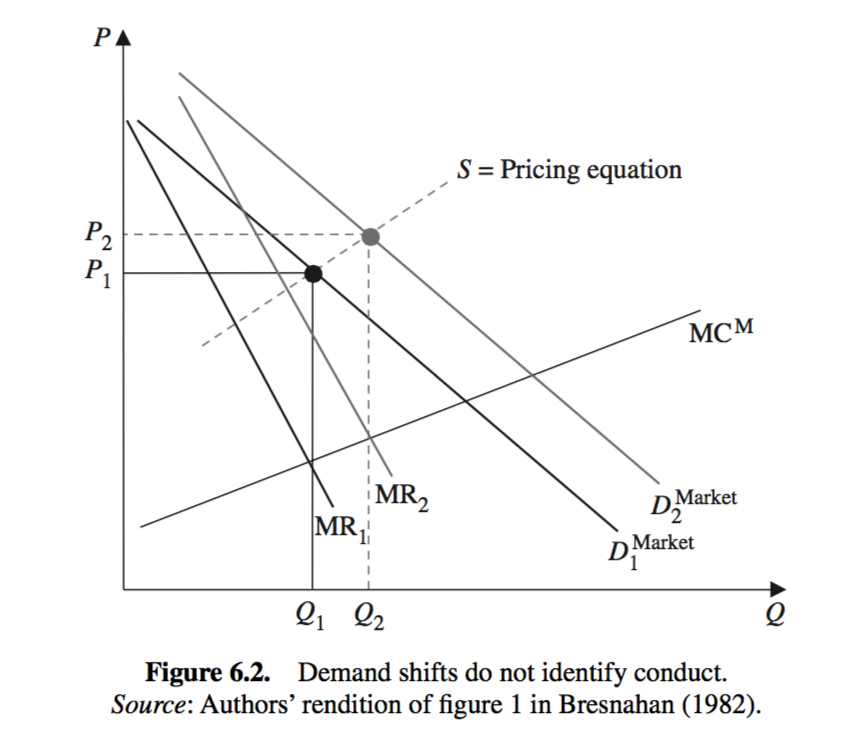
\includegraphics[width=0.8\linewidth]{figuretable/demandshift} 

}

\caption{Figure 6.2 of Davis (2006)}\label{fig:unnamed-chunk-25}
\end{figure}

\subsection{Identification of the Conduct Parameter: When Cost Data is
Available}\label{identification-of-the-conduct-parameter-when-cost-data-is-available}

\begin{itemize}
\tightlist
\item
  If there is reliable cost data, we can directly identify the marginal
  cost function:

  \begin{equation}
  MC(q_f) = \beta_0 + \beta_1 q_f + \beta_2 W + u^S,
  \end{equation}

  and so \(\beta_1\).
\item
  Then, in a combination with the identification of inverse demand
  function and pricing equation, \(\lambda\) is identified as:

  \begin{equation}
  \lambda = \alpha_1 \left(\frac{\beta_1}{N} - \gamma\right).
  \end{equation}
\end{itemize}

\subsection{Identification of the Conduct Parameter: When Cost Data is
Not
Available}\label{identification-of-the-conduct-parameter-when-cost-data-is-not-available}

\begin{itemize}
\tightlist
\item
  Remember the first-order condition:

  \begin{equation}
  \lambda Q P^{D\prime}(Q) + P^S(Q) = MC(q_f),
  \end{equation}

  where we can identify \(P^D(Q)\) and \(P^S(Q)\) if we have demand and
  cost shifters.
\item
  It is clear from this expression that we need a variation in
  \(P^{D\prime}(Q)\) with a fixed \(Q\) to identify \(\lambda\), i.e.,
  something that rotates the inverse demand function.
\item
  Intuition: If demand becomes more elastic, prices will decrease and
  quantity will increase in a market with a high degree of market power.
\end{itemize}

\subsection{Identification of the Conduct Parameter: Demand Rotater is
Available}\label{identification-of-the-conduct-parameter-demand-rotater-is-available}

\begin{itemize}
\tightlist
\item
  Let's formalize the idea.
\item
  To identify the conduct parameter, we needed a demand rotater:

  \begin{equation}
  P^D(Q) = \frac{\alpha_0}{\alpha_1} + \frac{1}{\alpha_1}Q + \frac{\alpha_2}{\alpha_1} X + \frac{\alpha_3}{\alpha_1} Q \underbrace{Z}_{\text{demand rotater}} +  \frac{1}{\alpha_1}u^D.
  \end{equation}
\item
  Inserting this into the first-order condition yields:

  \begin{equation}
  \frac{\lambda}{\alpha} Q_t (1 + \alpha Z_t)+ P^S(Q) = \beta_0 + \frac{\beta_1}{N} Q + \beta_2 W + u^s,
  \end{equation}
\item
  This determines the pricing equation:

  \begin{equation}
  \begin{split}
  P^S(Q) &= \beta_0 - \frac{\lambda}{\alpha_1} Q(1 + \alpha_3 Z_t) + \frac{\beta_1}{N} Q_t + \beta_2 W + u^S\\
  &\equiv \beta_0 + \gamma_1 Q + \gamma_2 Z Q + \beta_2 W + u^S,
  \end{split}
  \end{equation}

  where:

  \begin{equation}
  \gamma_1 \equiv \frac{\beta_1}{N} - \frac{\lambda}{\alpha_1}, \gamma_2 \equiv - \frac{\lambda \alpha_3}{\alpha_1}.
  \end{equation}

  \subsection{Identification of the Conduct Parameters: Demand Rotater
  is
  Available}\label{identification-of-the-conduct-parameters-demand-rotater-is-available}
\item
  If we have cost shifters \(W\), it can be used as instruments for
  \(Q\) in the inverse demand function to identify the demand parameters
  \((\alpha_0, \alpha_1, \alpha_2, \alpha_3)\).
\item
  If we have demand shifters \(X\), it can be used as instruments for
  \(Q\) in the pricing equation to identify the supply parameters
  \((\beta_0, \gamma_1, \gamma_2, \beta_2)\).
\item
  Now we can identify the \textbf{reduced-form} parameters
  \(\alpha_1, \alpha_3\) and \(\gamma_2\).
\item
  Then, we can not identify the conduct parameter:

  \begin{equation}
  \lambda = - \frac{\gamma_2 \alpha_1}{\alpha_3}.
  \end{equation}
\end{itemize}

\subsection{Identification of Conduct in Differentiated Product
Market}\label{identification-of-conduct-in-differentiated-product-market}

\begin{itemize}
\item
  Consider the identification of conduct when there are two
  differentiated substitutable products and companies compete in price
  \citep{Nevo1998}.
\item
  Are the prices determined independently or jointly?
\item
  The general first-order condition is:

  \begin{equation}
  \begin{split}
  &(p_1 - c_1) \frac{\partial Q_1(p)}{\partial p_1} + Q_1^S(p) + \Delta_{12}(p_2 - c_2) \frac{\partial Q_2 (p)}{\partial p_1} = 0\\
  &\Delta_{21}(p_1 - c_1)\frac{\partial Q_1(p)}{\partial p_2} + Q_2^S(p) + (p_2 - c_2) \frac{\partial Q_2 (p)}{\partial p_2} = 0,
  \end{split}
  \end{equation}

  where
\item
  \(\Delta_{12} = \Delta_{21} = 0\) if prices are determined
  independently.
\item
  \(\Delta_{12} = \Delta_{21} = 1\) if price are determined jointly.
\item
  Under what conditions can we identify \(\Delta_{12}\) and
  \(\Delta_{21}\)?
\item
  We will have to rotate \(\frac{\partial Q_1(p)}{\partial p_2}\) and
  \(\frac{\partial Q_2 (p)}{\partial p_1}\) while keeping the other
  variables at the same values.
\item
  \citet{Miller2017} infers \(\Delta\) after the MillerCoors, a joint
  venture of SABMiller PLC and Molson Coors Brewing, is formed.

  \begin{itemize}
  \tightlist
  \item
    The unobserved year-specific and region-specific cost shocks are
    identified from the outsiders and the unobserved product-specific
    cost shocks are assumed to be the same before and after the merger.
  \end{itemize}
\end{itemize}

\section{Merger Simulation}\label{merger-simulation}

\subsection{Unilateral and Coordinated Effects of a Horizontal
Merger}\label{unilateral-and-coordinated-effects-of-a-horizontal-merger}

\begin{itemize}
\tightlist
\item
  There are two effects associated with a merge episode:
\end{itemize}

\begin{enumerate}
\def\labelenumi{\arabic{enumi}.}
\tightlist
\item
  \textbf{Unilateral effect}:

  \begin{itemize}
  \tightlist
  \item
    The new merged firm usually have a unilateral incentive to raise
    prices above their pre-merger level.
  \item
    This unilateral effect may lead to the other firms to have an
    unilateral incentive to raise price, and the reaction continues to
    reach the new equilibrium.
  \item
    The latter chain reaction is sometimes called the
    \textbf{multi-lateral effect}.
  \item
    In economic theory, it is the price change when the same mode of
    competition (say, the Bertrand-Nash equilibrium) is played.
  \item
    \(\Delta\) is either 0 or 1: firms internalize the profits from
    owned product but do not internalize the other products.
  \end{itemize}
\item
  \textbf{Coordinated effect}:

  \begin{itemize}
  \tightlist
  \item
    After the merger, the mode of competition may change.
  \item
    For example, the tacit collusion becomes easier and it can happen.
  \item
    This effect, caused by the change in the mode of competition, is
    called the coordinated effect of a merger.
  \item
    In this case, the conduct parameters \(\Delta\) may take positive
    values for products owned by the rival firms.
  \end{itemize}
\end{enumerate}

\subsection{Merger Simulation}\label{merger-simulation-1}

\begin{itemize}
\tightlist
\item
  In merger simulation, we compute the equilibrium under different
  ownership structure.
\item
  This amounts to run a counterfactual simulation hypothetically
  changing the conduct parameter \(\Delta\).
\item
  The idea stems back to \citet{Farrell1990}, \citet{Werden1994},
  \citet{Hausman1994}.
\item
  Before running the simulation, you have to be very careful about the
  model assumptions:

  \begin{itemize}
  \tightlist
  \item
    In music industry, firms compete not in price but in advertisement.
  \item
    If technological diffusion is important, firms may set dynamic
    pricing.
  \end{itemize}
\item
  This is the first \textbf{counterfactual analysis} we study in this
  lecture.
\item
  The results are valid only if the modeling assumptions are correct.
\end{itemize}

\subsection{Quantifying the Unilateral
Effect}\label{quantifying-the-unilateral-effect}

\begin{itemize}
\tightlist
\item
  See \citet{Nevo2000c} and \citet{Nevo2001}.
\item
  There are \(J\) products, \(\mathcal{J} = \{1, \cdots, J\}\).
\item
  We can have multiple markets but we suppress the market index.
\item
  Firm \(f\) produces a set of products which we denote
  \(\mathcal{J}_f \subset \mathcal{J}\).
\item
  Let \(mc_j\) be the constant marginal cost of producing good \(j\).
\item
  Thus assuming a separable cost function.

  \begin{itemize}
  \tightlist
  \item
    We can relax this assumption for the estimation.
  \item
    However, once you admit that the costs can be non-separable, you
    will start to wonder what happens to the cost function if two firms
    merged and started to produce the two products that were previously
    produced by separate firms.
  \end{itemize}
\item
  Let \(D_j(p)\) be the demand for product \(j\) when the price vector
  is \(p\).
\item
  The problem for firm \(f\) given the price of other firms \(p_{-f}\)
  is:

  \begin{equation}
  \max_{p_f} \sum_{j \in \mathcal{J}_f} \Pi_j(p_f, p_{-f}) = \sum_{j \in \mathcal{J}_f} (p_j - mc_j) D_j(p_f, p_{-f}),
  \end{equation}

  where \(p_f = \{p_j\}_{j \in \mathcal{J}_f}\),
  \(p_{-f} = \{p_j\}_{j \in \mathcal{J} \setminus \mathcal{J}_f}\).
\end{itemize}

\subsection{Pre-Merger Equilibrium}\label{pre-merger-equilibrium}

\begin{itemize}
\tightlist
\item
  The first-order condition for firm \(f\) is:

  \begin{equation}
  D_k(p) + \sum_{j \in \mathcal{J}_f} (p_j - mc_j) \frac{\partial D_j(p)}{\partial p_k} = 0, \forall k \in \mathcal{J}_f.
  \end{equation}
\item
  Let \(\Delta_{jk}^{pre}\) takes 1 if same firm produces \(j\) and
  \(k\) and 0 otherwise before the merger.
\item
  The first-order condition can be written as:

  \begin{equation}
  D_k(p) + \sum_{j \in \mathcal{J}} \Delta_{jk}^{pre}(p_j - mc_j) \frac{\partial D_j(p)}{\partial p_k} = 0, \forall k \in \mathcal{J}_f.
  \end{equation}
\item
  In terms of the product share:

  \begin{equation}
  s_k(p) + \sum_{j \in \mathcal{J}} \Delta_{jk}^{pre}(p_j - mc_j) \frac{\partial s_j(p)}{\partial p_k} = 0, \forall k \in \mathcal{J}_f.
  \end{equation}
\item
  Let \(\Delta^{pre}\) be a \(J \times J\) matrix whose
  \((j, k)\)-element is \(\Delta_{jk}\).
\item
  At the end of the day, performing a merger simulation is to recompute
  the equilibrium with different ownership structure encoded in
  \(\Delta\).
\end{itemize}

\subsection{Post-Merger Equilibrium}\label{post-merger-equilibrium}

\begin{itemize}
\tightlist
\item
  Let \(\Omega^{pre}(p)\) is a matrix whose \((j, k)\)-element is:
\end{itemize}

\begin{equation}
- \frac{\partial s_{j}(p)}{\partial p_k} \Delta_{jk}^{pre}.
\end{equation}

\begin{itemize}
\tightlist
\item
  Then, by the first-order condition, the marginal cost should be:

  \begin{equation}
  mc = p - \Omega^{pre}(p)^{-1} s(p).
  \end{equation}
\item
  If the ownership structure \(\Delta^{pre}\) is changed to
  \(\Delta^{post}\), and \(\Omega^{pre}\) changed to \(\Omega^{post}\),
  the post-merger price is determined by solving the non-linear
  equation:

  \begin{equation}
  p^{post} = mc + \Omega^{post}(p^{post})^{-1}s(p^{post}).
  \end{equation}
\item
  The post-merger share is given by:

  \begin{equation}
  s^{post} = s(p^{post}).
  \end{equation}
\end{itemize}

\subsection{Consumer Surplus}\label{consumer-surplus}

\begin{itemize}
\tightlist
\item
  Suppose that the demand function is based on the mixed-logit model
  such that the indirect utility is:

  \begin{equation}
  u_{ijt} = x_{jt} \beta_i + \alpha_i p_{jt} + \xi_{j} + \xi_t + \Delta \xi_{jt} + \epsilon_{ijt},
  \end{equation}

  with \(\epsilon_{ijt}\) is drawn from i.i.d. Type-I extreme value
  distribution and the consumer-level heterogeneity:
\end{itemize}

\begin{equation}
\begin{pmatrix}
\alpha_i \\
\beta_i
\end{pmatrix}
= 
\begin{pmatrix}
\alpha\\
\beta
\end{pmatrix}
+ \Pi z_i + \Sigma \nu_i, \nu_i \sim N(0, I_{K + 1}).
\end{equation}

\begin{itemize}
\tightlist
\item
  Then, the compensated variation due to the price change for consumer
  \(i\) is:

  \begin{equation}
  CV_{it} = \frac{\ln (\sum_{j = 0}^J \exp(V_{ijt}^{post}) ) - \ln (\sum_{j = 0}^J \exp(V_{ijt}^{pre})) }{\alpha_i},
  \end{equation}

  where \(V_{ijt}^{post}\) and \(V_{ijt}^{pre}\) are indirect utility
  for consumer \(i\) to purchase good \(j\) at the prices after and
  before the merger.
\item
  This formula holds only if the price enters linearly in the indirect
  utility (no income effect).
\item
  For general case, see \citet{Small1981} and \citet{Mcfadden1995}.
\end{itemize}

\subsection{Quantifying the Coordinated
Effect}\label{quantifying-the-coordinated-effect}

\begin{itemize}
\tightlist
\item
  The repeated-game theory suggests that a collusion is sustainable if
  and only if it it incentive compatible: the collusion profit is no
  less than the deviation profit for each member of the collusion.
\item
  The theory provides a check list that affects the incentive
  compatibility such as the market share, cost asymmetry, and demand
  dynamics.
\item
  But it is often hard to judge the coordinated effects from these
  qualitative information, because mergers simultaneously change many
  factors and the factors may encourage or hinder collusion.
\item
  \citet{Miller2017} \textbf{retrospectively} studies the coordinated
  effect of a merger.
\item
  Is \textbf{prospective} analysis of coordinated effects possible as
  well as the analysis of unilateral effects?
\item
  If we can identify the demand and cost functions, we can calculate the
  collusion profits and deviation profits.
\item
  If we specify the collusion strategy, we can write down the incentive
  compatibility.
\item
  We can check how the incentive compatibility change when a
  hypothetical merger happens.
\item
  The problem is the identification of conduct: to identify the cost
  function, we need to know the conduct.
\item
  Thus, the stated strategy will work only if we have a data during
  which we are sure that there was no collusion, or there was a
  particular type of collusion.
\item
  \citet{Igami2018} use the detailed information of vitamin C cartel
  case and apply this approach.
\end{itemize}

\chapter{Entry and Exit}\label{entryexit}

\section{Motivations}\label{motivations-3}

\begin{itemize}
\tightlist
\item
  By studying the entry decisions of firms, we can identify the profit
  function including the entry cost of firms.
\item
  A profit function is the reduced-form parameter of the underlying
  demand function, cost function, and conduct parameters.
\item
  The profit function can be identified without assuming a particular
  conduct.
\item
  The parameter is informative enough to answer questions regarding the
  market structure and producer surplus.
\item
  In the last chapter, we discussed the identification of conduct, in
  which we learned that the exogenous change in the number of firms in a
  market gives some information about the conduct.
\item
  In the entry/exit analysis, we study the relationship between the
  market size, which exogenously changes the equilibrium number of
  firms, and the change in the market structure to infer the conduct.
\item
  Entry and exit is not all about firms.
\item
  The decision of launching a product is a sort of entry decision and
  the decision of abolishing a product is a sort of exit decision.
\item
  The framework in this chapter can be applied to a wider class of
  problems.
\item
  This chapter is mostly based on \citet{berry_identification_2006}.
\end{itemize}

\subsection{Entry Cost, Mode of Competition, and Market
Structure}\label{entry-cost-mode-of-competition-and-market-structure}

\begin{itemize}
\tightlist
\item
  Fixed and sunk entry costs and mode of competition are key
  determinants for market structure \citep{sutton_chapter_2007}.
\end{itemize}

\begin{figure}

{\centering 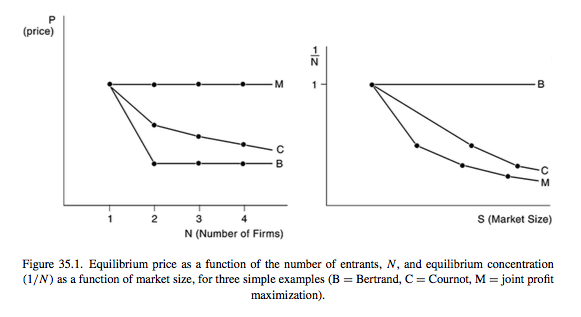
\includegraphics[width=0.8\linewidth]{figuretable/entrycost} 

}

\caption{Figure 1 of Sutton (2007)}\label{fig:unnamed-chunk-26}
\end{figure}

\begin{itemize}
\tightlist
\item
  The tougher the mode of competition, the less firms can earn enough
  profit to compensate the entry cost.
\item
  Therefore, the tougher the mode of competition, the number of firms in
  the market in the equilibrium cannot grow when the market size
  increases.
\end{itemize}

\subsection{Exogenous and Endogenous Entry
Cost}\label{exogenous-and-endogenous-entry-cost}

\begin{itemize}
\tightlist
\item
  \textbf{Exogenous fixed and sunk entry cost}:
\item
  The cost of entry is the same across modes of entry.
\item
  \textbf{Endogenous fixed and sunk entry cost}:
\item
  The cost differs across modes of entry.
\item
  For example, firms decide the quality of the product upon entering the
  market and the the cost of entry is increasing in the quality choice.
\item
  If endogenous fixed and sunk entry cost is relevant, the entry cost to
  compete with the incumbent and have a positive profit will increase as
  the the number of incumbent firms increases.
\item
  Therefore, the equilibrium firm number will be small and firm size
  will be large when endogenous fixed and sunk entry cost is relevant.
\end{itemize}

\section{Monopoly Entry}\label{monopoly-entry}

\subsection{Variable Profits and Fixed
Costs}\label{variable-profits-and-fixed-costs}

\begin{itemize}
\item
  Consider a cross-section of markets, with one potential entrant in
  each market.
\item
  Profits in market \(i\) are given by: \[
  \pi(x_i, F_i) \equiv v(x_i) - F_i.
  \]
\item
  \(v(x)\) is deterministic and \(F\) is random.
\item
  Typically, \(v(x)\) is interpreted as the variable profits and \(F\)
  as the fixed costs.
\item
  The potential entrant will enter market \(i\) if and only if: \[
  F_i \le v(x_i).
  \]
\item
  The parameters of interest are \(v\) and the distribution of \(F\),
  \(\Phi\).
\item
  In general, \(F\) in a market can be correlated with \(x\).
\end{itemize}

\subsection{Non-Identification}\label{non-identification}

\begin{itemize}
\tightlist
\item
  Assume that \(F\) is independent of \(x\).
\item
  Notice that a monotonic transformation of both sides of: \[
  F_i \le v(x_i).
  \] will not change the entry probability.
\item
  Therefore, without further restrictions, \(v\) and \(\Psi\) are at
  best identified only up to a monotonic transformation.
\end{itemize}

\subsection{Restrictions for
Identification.}\label{restrictions-for-identification.}

\begin{itemize}
\tightlist
\item
  Keep assuming that \(F\) is independent of \(x\).
\item
  Let \(p(x)\) is the observed entry probability at \(x\).
\end{itemize}

\begin{enumerate}
\def\labelenumi{\arabic{enumi}.}
\tightlist
\item
  \(v\) is known: Because \(v\) is the variable profit function, we can
  identify it directly from the demand function and cost function.

  \begin{itemize}
  \tightlist
  \item
    Let \(z = v(x)\). Then \(\Psi\) is identified at \(z\) by: \[
    \Psi(z)  = \mathbb{P}\{F \le z\} = \mathbb{P}\{F \le v[v^{-1}(z)]\} = p[v^{- 1}(z)].
    \]
  \end{itemize}
\item
  \(\Psi\) is known: Normalize the distribution of \(F\).

  \begin{itemize}
  \tightlist
  \item
    Then, \(v\) is identified at \(x\) by: \[
    v(x) = \Psi^{-1}[p(x)].
    \]
  \end{itemize}
\item
  Impose shape restrictions on \(v\) \citep{matzkin_nonparametric_1992}:

  \begin{itemize}
  \tightlist
  \item
    \(v(x)\) is homogeneous of degree 1 and there exists \(x_0\) such
    that \(v(x_0) = 1\). Then the functions \(v\) and \(\Psi\) are
    identified.
  \item
    Homogeneous of degree 1: \(v(z \cdot x) = z v(x)\).
  \item
    Let \(p(z, x_0)\) be the probability of entry at \(z\) and \(x_0\).
  \item
    Then, \(\Psi\) is identified at \(z\) by: \[
    \Psi(z) = \mathbb{P}\{F \le z\} = \mathbb{P}\{F \le z v(x_0)\} = p(z, x_0).
    \]
  \item
    Then, \(v\) is identified by the second argument.
  \end{itemize}
\end{enumerate}

\subsection{Homogeneous of Degree 1 Variable
Profits}\label{homogeneous-of-degree-1-variable-profits}

\begin{itemize}
\tightlist
\item
  Sufficient condition for the variable profit function to satisfy the
  stated condition:

  \begin{itemize}
  \tightlist
  \item
    Demand is proportional to the population.
  \item
    Marginal cost is constant.
  \item
    Then, the variable profit is the market size \(z\) times the
    per-capita profit.
  \item
    We can normalize \(v\) at a market of size \(z = 1\) by choosing
    arbitrary \(x_0\).
  \end{itemize}
\end{itemize}

\section{Complete-Information Homogeneous Oligopoly
Entry}\label{complete-information-homogeneous-oligopoly-entry}

\subsection{Variable and Fixed Costs}\label{variable-and-fixed-costs}

\begin{itemize}
\tightlist
\item
  \citet{bresnahan_entry_1991} pioneered the analysis of oligopoly entry
  models.
\item
  We observe a cross-section of markets in which we observe the number
  of homogeneous firms and other market-specific characteristics.
\item
  Let \(y_m\) be the number of firms in market \(m\).
\item
  Let \(v_{y_m}(x_m)\) is the variable profit per firm in a market with
  number of firms \(y_m\) and the market characteristics \(x_m\).
\item
  Let \(F_m\) be the market-specific fixed costs that are i.i.d. across
  markets with unknown distribution \(\Psi\).
\item
  If there are \(y_m\) firms in market \(m\), the profit per firm in the
  market is: \[
  \pi(y_m, x_m, F_m) \equiv v_{y_m}(x_m) - F_m.
  \]
\end{itemize}

\subsection{Equilibrium Condition}\label{equilibrium-condition}

\begin{itemize}
\item
  The unique Nash equilibrium in the number of firms in market \(m\) is
  determined by the following equilibrium condition: \[
  v_{y_m}(x_m) \ge F_m.
  \] \[
  v_{y_m + 1}(x_m) < F_m.
  \]
\item
  Under this equilibrium, the probability of observing \(y\) firms in a
  market of type \(x\) is: \[
  \mathbb{P}\{y = 0|x\} = 1 - \Psi[v_1(x)].
  \] \[
  \mathbb{P}\{y = 1|x\} = \Psi[v_1(x)] - \Psi[v_2(x)].
  \] \[
  \mathbb{P}\{y = 2|x\} = \Psi[v_2(x)] - \Psi[v_3(x)].
  \] \[
  \cdots
  \]
\item
  In other words, the probability of observing at least \(y\) firms in a
  market of type \(x\) is: \[
  \mathbb{P}\{y \ge 1|x\} = \Psi[v_1(x)].
  \] \[
  \mathbb{P}\{y \ge 2|x\} = \Psi[v_2(x)].
  \] \[
  \mathbb{P}\{y \ge 3|x\} = \Psi[v_3(x)].
  \] \[
  \cdots
  \]
\end{itemize}

\subsection{Identification under a Shape
Restriction}\label{identification-under-a-shape-restriction}

\begin{itemize}
\tightlist
\item
  The identification argument for each \(y\) is the same as the monopoly
  entry case.
\item
  For example, assume \(v_y(x) = z v_y(\tilde{x})\) and
  \(v_1(\tilde{x}_0) = 1\).
\item
  Let \(P_y(z, \tilde{x})\) be the observed probability that the number
  of firms is no less than \(y\) in market of type \(z, \tilde{x}\).
\item
  Then \(\Psi\) is identified at \(z\) by: \[
  \Psi(z) = \mathbb{P}\{F \le z\} = \mathbb{P}\{F \le z v_1(\tilde{x}_0)\} = P_1(z, \tilde{x}_0).
  \]
\item
  Then, the identification of \(v_y\) follows from: \[
  v_y(\tilde{x}) = \frac{\Psi^{-1}[P_y(z, \tilde{x})]}{z}.
  \]
\end{itemize}

\subsection{Log Likelihood Function}\label{log-likelihood-function}

\begin{itemize}
\tightlist
\item
  The log likelihood of observing \(\{y_m\}_{m = 1}^M\) given
  \(\{x_m\}_{m = 1}^M\) is: \[
  l(v, \Psi|\{y_m\}_{m = 1}^M,  \{x_m\}_{m = 1}^M) = \sum_{m = 1}^M \log\{\Psi[v_{y_m}(x_m)] - \Psi[v_{y_m + 1}(x_m)]\}.
  \]
\item
  This is a \textbf{ordered} model in \(y_m\).
\item
  If \(\Psi\) is a normal distribution, it is called an \textbf{ordered
  probit model}.
\end{itemize}

\section{Complete-Information Heterogeneous Oligopoly
Entry}\label{complete-information-heterogeneous-oligopoly-entry}

\subsection{Bivartiate Game with Heterogeneous
Profits}\label{bivartiate-game-with-heterogeneous-profits}

\begin{itemize}
\tightlist
\item
  We observe a cross-section of markets in which there are two potential
  entrants.
\item
  Let the profit of firm \(i\) in market \(m\) be: \[
  \begin{split}
  \pi_{im}(x_{im}, y_{jm}, f_{im}) & \equiv v(y_{jm}, x_{im}) - f_{im}\\
  &=v_{0i}(x_{im}) + y_{jm} v_{1i}(x_{im}) - f_{im}.
  \end{split}
  \]
\item
  \(y_{im}\) and \(y_{jm}\) are the indicators of entry of firm \(i\)
  and \(j\) in market \(m\).
\item
  \(x_{im}\) and \(x_{jm}\) are firm \(i\) and \(j\)'s characteristics
  in market \(m\).
\item
  \(f_{im}\) and \(f_{jm}\) are the fixed costs of firm \(i\) and \(j\)
  in market \(m\).
\item
  The second equation is without loss of generality because \(y_{jm}\)
  is a binary variable.
\item
  The competitive effect of firm \(j\) on \(i\) and the effect o firm
  \(i\) on \(j\) are asymmetric.
\item
  The parameters of interest are \(v_{0i}, v_{0j}, v_{1i}, v_{1j}\) and
  the joint distribution of \(f_{im}, f_{jm}\) conditional on \(x_{im}\)
  and \(x_{jm}\).
\item
  Firms \textbf{observe} both \(f_{im}, f_{jm}\) when they make
  decisions, but econometrician does not.
\end{itemize}

\subsection{Sampling Assumption and
Observations}\label{sampling-assumption-and-observations}

\begin{itemize}
\tightlist
\item
  We have a random sample of observations on markets where every
  observation is an observable realization of an equilibrium game played
  between firm \(i\) and \(j\).
\item
  Thus, we can observe:

  \begin{itemize}
  \tightlist
  \item
    \(\mathbb{P}\{0, 0|x\}\): the probability that a market of type
    \(x\) has no firm.
  \item
    \(\mathbb{P}\{1, 0|x\}\): the probability that a market of type
    \(x\) has firm \(i\) but not firm \(j\).
  \item
    \(\mathbb{P}\{0, 1|x\}\): the probability that a market of type
    \(x\) has firm \(j\) but not firm \(i\).
  \item
    \(\mathbb{P}\{1, 1|x\}\): the probability that a market of type
    \(x\) has both firms.
  \end{itemize}
\end{itemize}

\subsection{Identification Assuming Pure-Strategy
Equilibrium}\label{identification-assuming-pure-strategy-equilibrium}

\begin{itemize}
\item
  \citet{tamer_incomplete_2003} considers the identification when there
  are only two potential entrants and the pure-strategy Nash equilibrium
  is assumed.
\item
  Assume that the data is from a pure-strategy equilibrium.
\item
  Then, the probabilities \(\mathbb{P}\{0, 0|x\}\) and
  \(\mathbb{P}\{1, 1|x\}\) are written as: \[
  \mathbb{P}\{0, 0|x\} = \mathbb{P}\{f_{im} \ge v_{0i}(x_{im}), f_{jm} \ge v_{0j}(x_{jm})|x_{im}, x_{jm}\}.
  \] \[
  \mathbb{P}\{1, 1|x\} = \mathbb{P}\{f_{im} \le v_{0i}(x_{im}) + v_{1i}(x_{im}), f_{jm} \le v_{0j}(x_{jm}) + v_{1j}(x_{jm})|x_{im}, x_{jm}\}.
  \]
\item
  Assume that \((f_{im}, f_{jm})\) are distributed independently of
  \((x_{im}, x_{jm})\) with a joint distribution \(F\).
\item
  Assume that \(v_{0i}(x_{im}) = z_{im} v_0(\tilde{x}_{im})\) and
  \(v_{0j}(x_{jm}) = z_{jm} v_0(\tilde{x}_{jm})\).
\item
  Assume that \(v_{0i}(\tilde{x}_0) = v_{0j}(\tilde{x}_0) = 1\).
\item
  Assume that \(v_{1i}\) and \(v_{1j}\) are non-positive.
\item
  Assume that \(z_{im}| z_{jm}, \tilde{x}_{im}, \tilde{x}_{jm}\) has a
  distribution with support on \(\mathbb{R}\) and similar for
  \(z_{jm}\).
\item
  Then, \(F\) is identified by: \[
  \begin{split}
  \mathbb{P}\{f_{im} \ge z_{im}, f_{jm} \ge z_{jm}\} &= \mathbb{P}\{ f_{im} \ge z_{im} v_0(\tilde{x}_{0}), f_{jm} \ge z_{jm} v_0(\tilde{x}_{0})\}\\
  &= \mathbb{P}\{0, 0|z_{im}, \tilde{x}_0, z_{jm}, \tilde{x}_0\}.
  \end{split}
  \]
\item
  Then, push \(z_{jm} \to - \infty\) to get: \[
  \begin{split}
  \mathbb{P}\{f_{im} \ge z_{im} v_0(\tilde{x}_{im})\} &= \lim_{z_{jm} \to - \infty} \mathbb{P}\{f_{im} \ge z_{im} v_0(x_{im}), f_{jm} \ge z_{jm} v_0(x_{jm})\}\\
  &= \lim_{z_{jm} \to - \infty} \mathbb{P}\{0, 0|z_{im}, \tilde{x}_{im}, z_{jm}, \tilde{x}_{jm}\}
  \end{split}
  \]
\item
  Hence, \(v_{0}\) is identified by: \[
  v_0(\tilde{x}_{im}) = \frac{F^{-1}[\lim_{z_{jm} \to - \infty} \mathbb{P}\{0, 0|z_{im}, \tilde{x}_{im}, z_{jm}, \tilde{x}_{jm}\}]}{z_{im}}.
  \]
\item
  The identification of \(v_{1i}\) and \(v_{1j}\) are similar.
\end{itemize}

\subsection{Heterogeneous Independent Fixed
Costs}\label{heterogeneous-independent-fixed-costs}

\begin{itemize}
\tightlist
\item
  \citet{berry_estimation_1992} considers several extensions to the
  homogeneous oligopoly models.
\item
  Assume that the fixed costs are heterogeneous and independent across
  firms.

  \begin{itemize}
  \tightlist
  \item
    c.f. In homogeneous oligopoly model, the fixed costs were perfectly
    correlated across firms in a market.
  \end{itemize}
\item
  Assume that the characteristics can be firm-specific (that can include
  market-specific characteristics).
\item
  Assume that the variable profit function is homogeneous: \[
  \pi_{y}(x_m, F_{im}) = v_y(x_{im}) - F_{im}.
  \]
\item
  Assume that \(F\) is independent of \(x\).
\item
  Suppose that we observe the \textbf{number of potential entrants} in
  each market.
\item
  For example, in the airline industry, market is a city pair.
\item
  The potential entrants into an airline city pair were those with some
  service out of at least one of the endpoints of the city pair.
\item
  The variation in the number of potential entrants can be used to
  identify the model.
\item
  Define: \[
  \mu(x) = \mathbb{P}\{F_{im} < v_1(x)\}.
  \] \[
  \delta(x) = \mathbb{P}\{F_{im} < v_2(x)\}.
  \]
\item
  Suppose that we \textbf{know} that there only two potential entrants
  into a market.
\item
  Among such markets, we have: \[
  \mathbb{P}\{0, 0|x_1, x_2\} = [1 - \mu(x_1)] [1 - \mu(x_2)].
  \] \[
  \mathbb{P}\{1, 1|x_1, x_2\} = \delta(x_1) \delta(x_2).
  \]
\item
  If we set \(x_1 = x_2 = x\), then we have: \[
  \mathbb{P}\{0, 0|x, x\} = [1 - \mu(x)]^2.
  \] \[
  \mathbb{P}\{1, 1|x, x\} = \delta(x)^2.
  \]
\item
  They identify \(\mu\) and \(\delta\) at \(x\).
\item
  Under shape restrictions, we can identify \(v\) and \(\Psi\) as well.
\end{itemize}

\subsection{Heterogenous and Market-Level Correlated Fixed
Costs}\label{heterogenous-and-market-level-correlated-fixed-costs}

\begin{itemize}
\item
  Let \(\epsilon_m\) be the market-specific shock that affects the entry
  into market \(m\).
\item
  Conditional on \(\epsilon_m\), \(F_{im}\) are still independent across
  firms in a market.
\item
  Let \(\mu\) be: \[
  \mu(x, \epsilon_m) = \mathbb{P}\{F_{im} < v_1(x, \epsilon_m)\}.
  \]
\item
  When there is a market in which we \textbf{know} that there are only
  two potential entrants, the probability of observing \((0, 0)\)
  becomes: \[
  \mathbb{P}\{0, 0|x_1, x_2\} = \int [1 - \mu(x_1, \epsilon_m)] [1 - \mu(x_2, \epsilon_m)] d \Gamma(\epsilon_m).
  \]
\item
  Specifically, assume that: \[
  \epsilon_m 
  = 
  \begin{cases}
  0 & \text{   with probability   } \lambda \\
  1 & \text{   with probability   } 1 - \lambda.
  \end{cases}
  \]
\item
  Then, we in a market in which we \textbf{know} that there are only two
  potential entrants, the probability of observing \((0, 0)\) becomes:
  \[
  \mathbb{P}\{0, 0|x_1, x_2\} = \lambda [1 - \mu(x_1, 0)] [1 - \mu(x_2, 0)] + (1 - \lambda) [1 - \mu(x_1, 1)] [1 - \mu(x_2, 1)].
  \]
\item
  In general, in a market in which we \textbf{know} that there are only
  \(K\) potential entrants such that \(x_1 = \cdots x_K = x\), the
  probability of observing \((0, 0)\) becomes: \[
  \mathbb{P}\{0, 0|x, \cdots x\} = \lambda [1 - \mu(x, 0)]^K + (1 - \lambda) [1 - \mu(x, 1)]^K.
  \]
\item
  If there markets with \(K = 1, \cdots, \overline{K}\), we can
  construct \(\overline{K}\) equations with three unknowns \(\lambda\),
  \(\mu(x, 0)\), and \(\mu(x, 1)\).
\item
  Thus, the knowledge and the variation in the number of potential
  entrants help the identification.
\end{itemize}

\subsection{Inference Based On a Unique
Prediction}\label{inference-based-on-a-unique-prediction}

\begin{itemize}
\tightlist
\item
  \citet{berry_estimation_1992} develops a more general model built on
  the ideas above.
\item
  The key for his analysis is that he ensures that \textbf{there is a
  unique number of equilibrium entrants}.
\item
  This enables him to calculate the likelihood of observing a sequence
  of number of entrants, but at the cost of the generality of the
  underlying model.
\end{itemize}

\subsection{Entry in the Airline Industry: One-shot
Game}\label{entry-in-the-airline-industry-one-shot-game}

\begin{itemize}
\tightlist
\item
  Based on \citet{berry_estimation_1992}.
\item
  A market = a city pair market at a single point in time.
\item
  Consider a one-shot entry game that yields a network structure.
\item
  At the beginning of the period, each firm takes its overall network
  structure as given and decides whether to operate in a given city pair
  \textbf{independently} across markets.
\end{itemize}

\subsection{Entry in the Airline Industry: Profit
Function}\label{entry-in-the-airline-industry-profit-function}

\begin{itemize}
\tightlist
\item
  There are \(K_m\) potential entrants in market \(m\).
\item
  Let \(y_m\) be a strategy profile.
\item
  \(y_m = (y_{1m}, \cdots, y_{K_m m})'\), \(y_{im} \in \{0, 1\}\).
\item
  The profit function for firm \(i\) in market \(m\):

  \begin{equation}
  \pi_{im}(y_m, f_{im}) = v_m\left(N_{m}\right) - f_{im}.
  \end{equation}
\item
  \(N_{m} = \sum_{i = 1}^{K_m} y_{im}\).
\item
  \(v_m\) is strictly decreasing in \(N_m\).
\end{itemize}

\subsection{Entry in the Airline Industry: Profit
Function}\label{entry-in-the-airline-industry-profit-function-1}

\begin{itemize}
\tightlist
\item
  The common term is assumed to be: \[
  v_m(N) = x_m' \beta + h(\delta, N_m) + \rho u_{m}, 
  \]
\item
  \(x_m\) is the observed market characteristics, \(h(\cdot)\) is a
  function that is decreasing in \(N_m\), say, \(- \delta \ln (N_m)\).
\item
  \(u_m\) is the market characteristics that is observed by firms but
  not by econometrician.
\item
  The firm-specific term: \[
  f_{im} = z_{im}' \alpha + \sigma u_{im},
  \]
\item
  \(z_{im}\) is the observed firm characteristics.
\item
  A scale normalization: \(\sigma = \sqrt{1 - \rho^2}\)
  \(\Rightarrow var(\rho u_m + \sigma u_{im}) = 1\).
\end{itemize}

\subsection{Entry in the Airline Industry: Likelihood
Function}\label{entry-in-the-airline-industry-likelihood-function}

\begin{itemize}
\tightlist
\item
  The observed part: \[
  r_{im}(N) = x_m' \beta - \delta \ln (N_m) + z_{im}' \alpha. 
  \]
\item
  The unobserved part: \[
  \epsilon_{im} = \sqrt{1 - \rho^2} u_{im} + \rho u_{m}.
  \]
\end{itemize}

\subsection{Is the Equilibrium Number of Firms
Unique?}\label{is-the-equilibrium-number-of-firms-unique}

\begin{itemize}
\tightlist
\item
  Either of the following conditions are sufficient:
\item
  No firm-level unobserved heterogeneity: \(\rho = 1\).
\item
  No market-level unobserved heterogeneity: \(\rho = 0\).
\item
  The order of entry is predetermined, for example, the most profitable
  firms enter first.
\item
  The incumbent firms enter first.
\item
  Under either of the above assumptions, simulate the equilibrium number
  of firms in each market and match with the data.
\end{itemize}

\section{Multiple Prediction}\label{multiple-prediction}

\begin{itemize}
\tightlist
\item
  If we further generalize the model, we will suffer from the problem of
  \textbf{multiple prediction}.
\item
  First, even in \citet{berry_estimation_1992}'s framework, the identity
  of entrants were not uniquely predicted.
\item
  Second, if we allows for the asymmetric competitive effects, we will
  not have the unique number of equilibrium entrants.
\item
  Third, the uniqueness of the equilibria may not hold once we allow for
  the mixed-strategy Nash equilibria.
\item
  If we do not have the unique prediction on the endogenous variables,
  we cannot write down the likelihood function.
\end{itemize}

\subsection{Multiple Equilibria in Bivariate Game with Heterogenous
Profits}\label{multiple-equilibria-in-bivariate-game-with-heterogenous-profits}

\begin{itemize}
\tightlist
\item
  Return to \citet{tamer_incomplete_2003}'s bivariate game with
  heterogeneous profits.
\item
  Consider the pure-strategy Nash equilibrium when \(f_{im}, f_{jm}\)
  are realized.
\item
  \((0, 0)\) is a pure-strategy Nash equilibrium if: \[
  f_{im} \ge v_{0i}(x_{im});
  \] \[
  f_{jm} \ge v_{0j}(x_{jm}).
  \]
\item
  \((1, 1)\) is a pure-strategy Nash equilibrium if: \[
  f_{im} \le v_{0i}(x_{im}) + v_{1i}(x_{im});
  \] \[
  f_{jm} \le v_{0j}(x_{jm}) + v_{1j}(x_{jm}).
  \]
\item
  \((0, 1)\) is a pure-strategy Nash equilibrium if: \[
  f_{im} \ge v_{0i}(x_{im}) + v_{1i}(x_{im});
  \] \[
  f_{jm} \le v_{0j}(x_{jm}).
  \]
\item
  \((1, 0)\) is a pure-strategy Nash equilibrium if: \[
  f_{im} \le v_{0i}(x_{im});
  \] \[
  f_{jm} \ge v_{0j}(x_{jm}) + v_{1j}(x_{jm}).
  \]
\item
  In a certain region of \(f_{im}, f_{jm}\), there are multiple
  equilibria.
\end{itemize}

\subsection{Multiple Prediction in Bivariate Game with Heterogenous
Profits}\label{multiple-prediction-in-bivariate-game-with-heterogenous-profits}

\begin{itemize}
\tightlist
\item
  In the orange region, we have multiple pure-strategy equilibria.
\item
  If we allow for mixed-strategy equilibria, the region of
  \(f_{im}, f_{jm}\) on which there are multiple equilibria will
  increase. \textbackslash{}begin\{figure\}
\end{itemize}

\{\centering 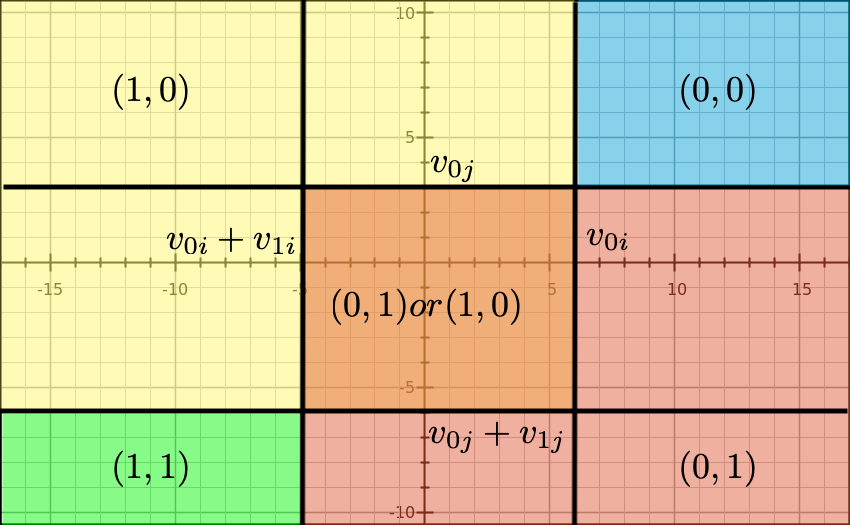
\includegraphics[width=0.8\linewidth]{figuretable/bivariateentry}

\}

\textbackslash{}end\{figure\} - In this example, we can write the
likelihood of the number of equilibrium entrants: - \(2\): green area. -
\(1\): yellow, orange, and red areas. - \(0\): blue area. - However, we
cannot write the likelihood of the strategy profile. - \((1, 1)\): green
area. - \((0, 1)\): \(\ge\) red area, \(\le\) orange and red area. -
\((1, 0)\): \(\ge\) yellow area, \(\le\) orange and yellow area. -
\((0, 0)\): blue area.

\subsection{Inference Based on Moment
Inequalities}\label{inference-based-on-moment-inequalities}

\begin{itemize}
\tightlist
\item
  According to the theory, we have: \[
  \mathbb{P}\{0, 0|x\} = \mathbb{P}\{f_{i} \ge v_{0i}(x_{i}), f_{j} \ge v_{0j}(x_{j})\} \equiv H(0, 0|x).
  \]
\end{itemize}

\[
\mathbb{P}\{1, 1|x\} = \mathbb{P}\{f_{i} \le v_{0i}(x_{i}) + v_{1i}(x_{i}), f_{j} \le v_{0j}(x_{j}) + v_{1j}(x_{j}) \} \equiv H(1, 1|x).
\]

\[
\mathbb{P}\{0, 1|x\} \ge \mathbb{P}\{f_{i} \ge v_{0i}, f_{j} \le v_{0j}\} + \mathbb{P}\{f_{i} \ge v_{0i} + v_{1i}, f_{j} \le v_{0j} + v_{1j}\} \equiv \underline{H}(0, 1|x).
\]

\[
\mathbb{P}\{0, 1|x\} \le \underline{H}(0, 1|x) + \mathbb{P}\{v_{0i} + v_{1i} \le f_{i} \le v_{0i}, v_{0j} + v_{1j} \le f_{j} \le f_{0j}\} \equiv \overline{H}(0, 1|x).
\]

\[
\mathbb{P}\{1, 0|x\} \ge \mathbb{P}\{f_{j} \ge v_{0j}, f_{i} \le v_{0i}\} + \mathbb{P}\{f_{j} \ge v_{0j} + v_{1j}, f_{i} \le v_{0i} + v_{1i}\} \equiv \underline{H}(1, 0|x).
\]

\[
\mathbb{P}\{1, 0|x\} \le \underline{H}(0, 1|x) + \mathbb{P}\{v_{0} + v_{1i} \le f_{i} \le v_{0i}, v_{0j} + v_{1j} \le f_{j} \le f_{0j}\} \equiv \overline{H}(1, 0|x).
\]

\begin{itemize}
\tightlist
\item
  The parameters should satisfy the moment conditions: \[
  \mathbb{P}\{0, 0|x\} - H(0, 0|x) = 0;
  \] \[
  \mathbb{P}\{1, 1|x\} - H(1, 1|x) = 0;
  \] \[
  \min\left\{\mathbb{P}\{0, 1|x\} - \underline{H}(0, 1|x), 0\right\} = 0;
  \] \[
  \max\left\{\mathbb{P}\{0, 1|x\} - \overline{H}(0, 1|x), 0\right\} = 0;
  \] \[
  \min\left\{\mathbb{P}\{1, 0|x\} - \underline{H}(1, 0|x), 0\right\} = 0;
  \] \[
  \max\left\{\mathbb{P}\{1, 0|x\} - \overline{H}(1, 0|x), 0\right\} = 0;
  \]
\item
  We can estimate the parameters with the GMM method using the above
  modified moment conditions.
\item
  Inference based on the moment inequalities are found in
  \citet{andrews_inference_2010}.
\item
  \citet{ciliberto_market_2009} study the entry exit of airlines when
  there are heterogeneous competitive effects using the above approach.
\end{itemize}

\section{Incompelete-Information Heterogenous Oligopoly
Entry}\label{incompelete-information-heterogenous-oligopoly-entry}

\subsection{Bivariate Case}\label{bivariate-case}

\begin{itemize}
\tightlist
\item
  There are two potential entrants.
\item
  Let the profit of firm \(i\) in market \(m\) be: \[
  \begin{split}
  \pi_{im}(x_{im}, y_{jm}, f_{im}) & \equiv v(y_{jm}, x_{im}) - f_{im}\\
  &=v_{0i}(x_{im}) + y_{jm} v_{1i}(x_{im}) - f_{im}.
  \end{split}
  \]
\item
  \(y_{im}\) and \(y_{jm}\) are the indicators of entry of firm \(i\)
  and \(j\) in market \(m\).
\item
  \(x_{im}\) and \(x_{jm}\) are firm \(i\) and \(j\)'s characteristics
  in market \(m\).
\item
  \(f_{im}\) and \(f_{jm}\) are the fixed costs of firm \(i\) and \(j\)
  in market \(m\).
\item
  The second equation is without loss of generality because \(y_{jm}\)
  is a binary variable.
\item
  The competitive effect of firm \(j\) on \(i\) and the effect o firm
  \(i\) on \(j\) are asymmetric.
\item
  The parameters of interest are \(v_{0i}, v_{0j}, v_{1i}, v_{1j}\) and
  the joint distribution of \(f_{im}, f_{jm}\) conditional on \(x_{im}\)
  and \(x_{jm}\).
\item
  Firm \(i\) \textbf{observe} both \(f_{im}\) but \textbf{not}
  \(f_{jm}\) when it makes decision.
\item
  Firm \(j\) \textbf{observe} both \(f_{jm}\) but \textbf{not}
  \(f_{im}\) when it makes decision.
\item
  Econometrican does not observe either of them.
\item
  The joint distribution of \(f_{im}, f_{jm}\) is \(F\) (independent of
  \(x\)).
\end{itemize}

\subsection{The Equilibrium Strategy and
Belief}\label{the-equilibrium-strategy-and-belief}

\begin{itemize}
\tightlist
\item
  The equilibrium strategy becomes a step function that decreases in a
  threshold: \[
  y_{im} = 1\{f_{im} \le t_{im}\}.
  \] \[
  y_{jm} = 1\{f_{jm} \le t_{jm}\}.
  \]
\item
  Suppose that firm \(i\) believes that \(f_{jm}\) has a distribution of
  \(G_{jm}^{im}\) and firm \(j\) believes that \(f_{im}\) has a
  distribution of \(G_{im}^{jm}\).
\item
  Usually, we assume a common and objective prior:
  \(G_{jm}^{im}(\epsilon_{jm}) = F(\epsilon_{jm}|\epsilon_{im})\) and
  \(G_{im}^{jm}(\epsilon_{im}) = F(\epsilon_{im}|\epsilon_{jm})\).
\item
  When firm \(j\) follows strategy \(t_{jm}\), the expected payoff for
  firm \(i\) to enter is: \[
  [v_{0i}(x_{im}) - f_{im}][1 - G_{jm}^{im}(t_{jm})] + [v_{0i}(x_{im}) + v_{1i}(x_{im} - f_{im})] G_{jm}^{im}(t_{jm}).
  \]
\item
  Thus, the threshold \(t_{im}\) is determined by: \[
  [v_{0i}(x_{im}) - t_{im}][1 - G_{jm}^{im}(t_{jm})] + [v_{0i}(x_{im}) + v_{1i}(x_{im} - t_{im})] G_{jm}^{im}(t_{jm}) = 0.
  \]
\item
  In the same way, the threshold \(t_{jm}\) is determined by: \[
  [v_{0j}(x_{jm}) - t_{jm}][1 - G_{im}^{jm}(t_{im})] + [v_{0j}(x_{jm}) + v_{1j}(x_{jm} - t_{jm})] G_{im}^{jm}(t_{im}) = 0.
  \]
\item
  This system of equations can have multiple solution.
\end{itemize}

\subsection{Equilibrium Selection and
Likelihood}\label{equilibrium-selection-and-likelihood}

\begin{itemize}
\tightlist
\item
  If we specify the equilibrium selection rule
  \(\mathbb{P}(t_{im}, t_{jm}|x_{im}, x_{jm}, f_{im}, f_{jm})\), then we
  can specify the likelihood of observing \((0, 0)\), \((0, 1)\),
  \((1, 0)\), and \((1, 1)\).
\item
  If we do not, we will only have bounds on the likelihood of observing
  \((0, 0)\), \((0, 1)\), \((1, 0)\), and \((1, 1)\).
\item
  Another way is to assume that \textbf{the same equilibrium
  \(t_{im}^*(x_{im}, x_{jm}), t_{jm}^*(x_{im}, x_{jm})\) holds across
  markets}.
\item
  Then, the across market relative frequency of entries conditional on
  \(x_{im}, x_{jm}\) gives the estimates of the entry probabilities: \[
  \widehat{G}_{im}(x_{im}, x_{jm}) \approx G_{im}^{jm}[t^*_{im}(x_{im}, x_{jm})],
  \] \[
  \widehat{G}_{jm}(x_{im}, x_{jm}) \approx G_{jm}^{im}[t_{jm}^*(x_{im}, x_{jm})],
  \] for each \(x_{im}, x_{jm}\).
\item
  The estimated distribution has to solve: \[
  \widehat{G}_{im}(x_{im}, x_{jm}) = \mathbb{P}\{[v_{0i}(x_{im}) - f_{im}][1 - \widehat{G}_{jm}(x_{im}, x_{jm})] + [v_{0i}(x_{im}) + v_{1i}(x_{im}) - f_{im}] \widehat{G}_{jm}(x_{im}, x_{jm}) > 0\}.
  \] \[
  \widehat{G}_{jm}(x_{im}, x_{jm}) = \mathbb{P}\{[v_{0j}(x_{jm}) - f_{jm}][1 - \widehat{G}_{im}(x_{im}, x_{jm})] + [v_{0j}(x_{jm}) + v_{1j}(x_{jm}) - f_{jm}] \widehat{G}_{im}(x_{im}, x_{jm}) > 0\}.
  \]
\item
  We find parameters \(v_{0i}, v_{0j}, v_{1i}, v_{1j}, F\) that solve
  this system of equations.
\item
  The ``same equilibrium'' assumption is hardly justified, but is often
  used in the empirical studies.
\end{itemize}

\chapter{Dynamic Decision Model}\label{dynamics}

\section{Motivations}\label{motivations-4}

\begin{itemize}
\tightlist
\item
  The model is \textbf{dynamic} if there is an \textbf{endogenous state
  variable}, a state variable that is affected by an action of a player
  in the past.
\item
  There are many cases where the decision makers have to take into
  account the dynamic effects of their actions.
\item
  \textbf{Payoff linkages}:

  \begin{itemize}
  \tightlist
  \item
    Storable good: Next week's demand for a detergent depends on how
    many bottles consumers purchase and consume this week. The latter
    depends on this week's price and the price schedule of the
    detergent. The stock of the detergent consumers hold is an
    endogenous state variable.
  \item
    Learning by doing: The productivity of a firm next year can be
    higher if the firm produced more this year because the firm can
    learn from the experience. The cummulative production level is an
    endogenous state variable.
  \end{itemize}
\item
  \textbf{Information linkages}:

  \begin{itemize}
  \tightlist
  \item
    Uncertainty about the quality: If a consumer is uncertain about the
    quality of a product but can learn from experiencing the product,
    next seaons's demand for the product depends on how many consumers
    purchace and experience the product this season. The latter depends
    on this season's price and the price schedule of the product.
  \end{itemize}
\item
  \textbf{Strategic linkages}:

  \begin{itemize}
  \tightlist
  \item
    Tacit collusion: If a firm deviates from the collusive price, the
    price war will start. Then, the history of the prices is the
    endogenous state variable.
  \end{itemize}
\end{itemize}

\section{Single-Agent Model}\label{single-agent-model}

\subsection{Setting}\label{setting}

\begin{itemize}
\tightlist
\item
  This model originates at \citet{rust_optimal_1987}, while the setting
  and the notation follows \citet{pesendorfer_asymptotic_2008}.
\item
  We start from a simple set-up:
\item
  Single agent.
\item
  Infinite-horizon discrete time.

  \begin{itemize}
  \tightlist
  \item
    Time is \(t = 1, 2, \cdots, \infty\).
  \end{itemize}
\item
  Finitely many choices.

  \begin{itemize}
  \tightlist
  \item
    There are \(K + 1\) actions \(A = \{0, 1, \cdots, K\}\).
  \end{itemize}
\item
  Finite state space.

  \begin{itemize}
  \tightlist
  \item
    There are \(L\) states \(S = \{1, \cdots, L\}\).
  \end{itemize}
\item
  Markovian state transition.
\end{itemize}

\subsection{Timing of the Model}\label{timing-of-the-model}

\begin{itemize}
\tightlist
\item
  At period \(t\):
\item
  State \(s_t \in S\) is publicly observed.
\item
  Choice-specific profitability shocks
  \(\epsilon_t \in \mathbb{R}^{K + 1}\) are realized according to
  \(F(\cdot|s_t)\) and privately observed.
\item
  Choice \(a_t \in A\) is made.
\item
  State evolves according to a transition probability:

  \begin{equation}
  g(a, s, s') \equiv \mathbb{P}\{s_{t + 1} = s'|s_t = s, a_t = a\},
  \end{equation}
\item
  Thus, the transition law only depends on today's state and action, but
  not on the past history.
\end{itemize}

\begin{equation}
G \equiv 
\begin{pmatrix}
g(0, 1, 1) & \cdots & g(0, 1, L)\\
\vdots & & \vdots \\
g(0, L, 1) & \cdots & g(0, L, L)\\
& \vdots & \\
g(K, 1, 1) & \cdots & g(K, 1, L)\\
\vdots & & \vdots \\
g(K, L, 1) & \cdots & g(K, L, L)\\
\end{pmatrix}.
\end{equation}

\subsection{Period Payoff}\label{period-payoff}

\begin{itemize}
\tightlist
\item
  When the state is \(s_t\), action is \(a_t\), and the profitability
  shocks are \(\epsilon_t\), the period payoff is:

  \begin{equation}
  \pi(a_t, s_t) + \sum_{k = 1}^K \epsilon_{tk} 1\{a_t = k\},
  \end{equation}
\item
  \(\pi(a_t, s_t)\) is the mean \textbf{choice-specific period payoff}.
\item
  \(\epsilon_t\) is assuemd to be i.i.d. across times and is drawn from
  \(F\).
\item
  Let: \[
  \epsilon_{t a_t} \equiv \sum_{k = 1}^K \epsilon_{tk} 1\{a_t = k\},
  \] be the choice-specific profitability shock.
\item
  Let \(\Pi\) summarize the choice-specific period payoffs at each
  state:

  \begin{equation}
  \Pi =
  \begin{pmatrix}
  \pi(0, 1)\\
  \vdots \\
  \pi(0, L)\\
  \vdots \\
  \pi(K, 1)\\
  \vdots \\
  \pi(K, L)\\
  \end{pmatrix}.
  \end{equation}
\item
  The \textbf{payoff} is the discounted sum of future payoffs with
  discount factor \(\beta < 1\).
\item
  \(\Pi\) is one of the parameters of interest.
\end{itemize}

\subsection{Markovian Framework}\label{markovian-framework}

\begin{itemize}
\tightlist
\item
  The strategy is in general a mapping from the \textbf{entire} history
  to the action set.
\item
  We restrict the set of possible strategies to \textbf{Markovian
  strategies} \(a(\epsilon_t, s_t)\) that only depends on the latest
  realization of states \(\epsilon_t, s_t\), i.e., the behavior does not
  depend on the past states, conditional on today's states.
\item
  The Markovian strategy is introduced by \citet{maskin_theory_1988-1}.
  But their model is slightly different from the current mode. They
  considered an oligopoly model in which only one firm can move at one
  time and his/her action depends only on the rival's latest move. The
  current single-agent model can be regarded as a version of
  \citet{maskin_theory_1988-1}'s model such that the rival is replaced
  with the nature.
\end{itemize}

\subsection{Belief}\label{belief}

\begin{itemize}
\tightlist
\item
  When a play makes a decision, s/he should have some belief about the
  future \(\epsilon_t, s_t\), and \(a_t\).
\item
  We usually assume the \textbf{rational expectation}: the play knows
  the equilibrium distribution of these future variables and use it as
  his/her belief.
\item
  The distribution of \(\epsilon_t\) and \(s_t\) is believed to follow
  \(F\) and \(G\).
\item
  Let \(\sigma(a|s)\) be the player's belief about the possibility of
  taking \(a\) when the realized state is \(s\), which may or may not
  coincide with the equilibrium probability.
\item
  Let \(\sigma\) stack them up as:

  \begin{equation}
  \sigma = 
  \begin{pmatrix}
  \sigma(0|1)\\
  \vdots\\
  \sigma(0|L)\\
  \vdots\\ 
  \sigma(K|1)\\
  \vdots\\ 
  \sigma(K|L)
  \end{pmatrix}.
  \end{equation}
\end{itemize}

\subsection{Decision Problem}\label{decision-problem}

\begin{itemize}
\tightlist
\item
  The agent chooses strategy \(a(\cdot, \cdot)\) such that:

  \begin{equation}
  \begin{split}
  \max_{a(\cdot, \cdot)} & \pi[a(\epsilon_0, s_0), s_0] + \epsilon_{0 a(\epsilon_0, s_0)}\\
  &+ \mathbb{E}\Bigg\{ \sum_{t = 1}^\infty \beta^t \Bigg[\pi(a_t, s_t) + \epsilon_{t a(\epsilon_t, s_t)}\Bigg]\Bigg|s_0, a(\epsilon_0, s_0)\Bigg\}
  \end{split}
  \end{equation}
\item
  The expectation is taken with respect to his/her belief.
\end{itemize}

\subsection{Value Function and Ex-ante Value
Function}\label{value-function-and-ex-ante-value-function}

\begin{itemize}
\tightlist
\item
  When the belief about the future behavior is \(\sigma\), then the
  value function associated with the belief is defined as:

  \begin{equation}
  \begin{split}
  &V(\sigma, s_0, \epsilon_0)\\
  &= \sum_{a \in A} \sigma(a|s_0) \Bigg\{\pi(a, s_0) + \epsilon_{0a} + \mathbb{E}\Bigg[ \sum_{t = 1}^\infty \beta^t \sum_{a \in A}\sigma(a|s_t)\Bigg(\pi(a, s_t) + \epsilon_{ta}\Bigg)\Bigg|s_0, a\Bigg] \Bigg\}.
  \end{split}
  \end{equation}
\item
  It has the recursive structure as:

  \begin{equation}
  \begin{split}
  &V(\sigma, s_0, \epsilon_0)\\
  & = \sum_{a \in A} \sigma(a|s_0) \Bigg\{\pi(a, s_0) + \epsilon_{0a} + \beta \mathbb{E}\Bigg[V(\sigma, s_1, \epsilon_1)\Bigg|s_0, a\Bigg]\Bigg\}\\
  & = \sum_{a \in A} \sigma(a|s_0) \Bigg\{\pi(a, s_0) + \epsilon_{0a} + \beta \sum_{s_1 \in S} V(\sigma, s_1, \epsilon_1)g(a, s_0, s_1)\Bigg\}.
  \end{split}
  \end{equation}
\item
  \(V(\sigma, s, \epsilon)\) is the value function after the
  profitablity shock \(\epsilon\) is realized.
\item
  On the other hand, we define the \textbf{ex-ante value function} under
  belief \(\sigma\) as:

  \begin{equation}
  V(\sigma, s) = \mathbb{E}\{V(\sigma, s, \epsilon)|s\}.
  \end{equation}
\end{itemize}

\subsection{Choice-specific Value
Function}\label{choice-specific-value-function}

\begin{itemize}
\tightlist
\item
  When the current state and profitability shocks are \(s\) and
  \(\epsilon\) and the belief about the future behavior is \(\sigma\),
  we define the \textbf{choice-specific} value function for an agent in
  a period as follows:

  \begin{equation}
  \begin{split}
  V(\sigma, a, s, \epsilon) &= \pi(a , s) + \epsilon_a + \beta \sum_{s' \in S} V(\sigma, s') g(a, s, s')\\
   &= \underbrace{\pi(a , s) + \beta \sum_{s' \in S} V(\sigma, s') g(a, s, s')}_{v(\sigma, a, s)} + \epsilon_a.
  \end{split}
  \end{equation}
\item
  We call \(v(\sigma, a, s)\) be the \textbf{choice-specific} mean value
  function with belief \(\sigma\).
\item
  \(V(\sigma, s, \epsilon)\), \(V(\sigma, s)\),
  \(V(\sigma, a, s, \epsilon)\), and \(v(\sigma, a, s)\) are all
  different, abusing the notation.
\end{itemize}

\subsection{Optimality Condition}\label{optimality-condition}

\begin{itemize}
\tightlist
\item
  When the state and profitability shocks are \(s\) and \(\epsilon\),
  \(a\) is the optimal choice if and only if:

  \begin{equation}
  v(\sigma, a, s) + \epsilon_{a} \ge v(\sigma, a', s) + \epsilon_{a'}, \forall a' \in A.
  \end{equation}
\item
  This condition looks similar to the optimality condition in the static
  discrete choice model.
\item
  The only difference from the static discrete choice model is that the
  mean indirect utility is the sum of the choice-specific mean profit
  and the discounted continuation value.
\item
  Thus, as long as the mean choice-specific value function for given
  parameters can be computed, the following simulation and estimation
  procedure will be similar to the static discrete chocie model.
\end{itemize}

\subsection{Optimal Conditional Choice
Probability}\label{optimal-conditional-choice-probability}

\begin{itemize}
\tightlist
\item
  From the previous optimality condition, we can define the
  \textbf{optimal conditional choice probability} with belief \(\sigma\)
  as:

  \begin{equation}
  \begin{split}
  p(a|s, \sigma) &\equiv \mathbb{P}\{v(\sigma, a, s) + \epsilon_{a} \ge v(\sigma, a', s) + \epsilon_{a'}, \forall a' \in A\}\\
  &= \int \prod_{a' \neq a} 1\{v(\sigma, a, s) + \epsilon_{a} \ge v(\sigma, a', s) + \epsilon_{a'}\} dF\\
  &\equiv \Psi(\sigma, a, s).
  \end{split}
  \end{equation}
\item
  \(\Psi(\sigma, a, s)\) maps the tuple of action, state and belief to
  the optimal conditional choice probability of the action given the
  state and the belief.
\end{itemize}

\subsection{Optimality Condition}\label{optimality-condition-1}

\begin{itemize}
\tightlist
\item
  Let \(p\) and \(\Psi\) be:

  \begin{equation}
  p = 
  \begin{pmatrix}
  p(0|1)\\
  \vdots\\
  p(0|L)\\
  \vdots\\
  p(K|1)\\
  \vdots\\
  p(K|L)
  \end{pmatrix},
  \end{equation}
\end{itemize}

\begin{equation}
\Psi(\sigma) = 
\begin{pmatrix}
\Psi(\sigma, 0, 1)\\
\vdots\\
\Psi(\sigma, 0, L)\\
\vdots\\
\Psi(\sigma, K, 1)\\
\vdots\\
\Psi(\sigma, K, L)
\end{pmatrix}.
\end{equation}

\begin{itemize}
\tightlist
\item
  The optimality condition with respect to the conditional choice
  probabilities given the belief is written as:

  \begin{equation}
  p = \Psi(\sigma).
  \end{equation}
\item
  The rational expectation hypothesis requires that the belief about the
  future behavior coincides with the optimal conditional choice
  probability, i.e.:

  \begin{equation}
  p = \Psi(p).
  \end{equation}
\item
  The optimal conditional choice probability under the rational
  expectation hypothesis is characterized as a fixed point of mapping
  \(\Psi\).
\end{itemize}

\subsection{Mapping from a Conditional Choice Probability to an Ex-ante
Value
Function}\label{mapping-from-a-conditional-choice-probability-to-an-ex-ante-value-function}

\begin{itemize}
\tightlist
\item
  Inserting \(\sigma = p\), we obtain a mapping from an optimal
  conditional choice probability to an ex-ante value function such as:

  \begin{equation}
  \begin{split}
  V(s) &= \mathbb{E}\{V(s, \epsilon)|s\}\\
  &= \mathbb{E}\left[ \sum_{t = 0}^\infty \beta^t \sum_{a \in A}p(a|s_t)\left[\pi(a, s_t) + \epsilon_{ta}\right]\Bigg|s_0, a\right]\\
  &\equiv \varphi(p, s).
  \end{split}
  \end{equation}
\end{itemize}

\subsection{Mapping from an Ex-ante Value Function to an Optimal
Conditional Choice
Probability}\label{mapping-from-an-ex-ante-value-function-to-an-optimal-conditional-choice-probability}

\begin{itemize}
\tightlist
\item
  On the other hand, we can derive a mapping from an ex-ante value
  function to an optimal conditional choice probability such as:

  \begin{equation}
  \begin{split}
  p(a|s) = \mathbb{P}\Bigg\{&\pi(a , s) + \beta \sum_{s' \in S} V(s') g(a, s, s') + \epsilon_a \ge\\
  &\pi(a' , s) + \beta \sum_{s' \in S} V(s') g(a', s, s') + \epsilon_{a'}, \forall a' \in A \Bigg\}\\
  &\equiv \Lambda(V, s).
  \end{split}
  \end{equation}
\end{itemize}

\subsection{The Optimality Conditions}\label{the-optimality-conditions}

\begin{itemize}
\tightlist
\item
  Composing these two mappings, we can write down the optimality
  condition as the fixed-point for ex-ante value functions:

  \begin{equation}
  V = \varphi(p) = \varphi[\Lambda(V)] \equiv \Phi(V).
  \end{equation}
\item
  Or as the fixed-point for the optimal conditional choice
  probabilities: \[
  p = \Lambda(V) = \Lambda[\varphi(p)] \equiv \Psi(p).
  \]
\end{itemize}

\subsection{Fixed-point Algorithm}\label{fixed-point-algorithm}

\begin{itemize}
\tightlist
\item
  If \(\epsilon\) is drawn from an i.i.d. type-I extreme value
  distribution, we can derive the mapping from the ex-ante value
  function to the conditional choice probability in the closed form:

  \begin{equation}
  \begin{split}
  \Lambda(V, s) &= \mathbb{P}\{\pi(a , s) + \beta \sum_{s' \in S} V(s') g(a, s, s') + \epsilon_{a} \ge\\
   & \pi(a' , s) + \beta \sum_{s' \in S} V(s') g(a', s, s') + \epsilon_{a'}, \forall a' \in A\}\\
  &=\frac{\exp[\pi(a , s) + \beta \sum_{s' \in S} V(s') g(a, s, s')]}{\sum_{a' \in A} \exp[\pi(a' , s) + \beta \sum_{s' \in S} V(s') g(a', s, s')]}.
  \end{split}
  \end{equation}
\item
  Moreover, we can also derive the mapping from the ex-ante value
  function to the ex-ante value function as follows:

  \begin{equation}
  \begin{split}
  \Phi(V) &= \mathbb{E}\{\max_{a \in A} \pi(a , s) + \beta \sum_{s' \in S} V(s') g(a, s, s') + \epsilon_{a}\} \\
  &=\log \Bigg\{\sum_{a \in A} \exp[\pi(a , s) + \beta \sum_{s' \in S} V(s') g(a, s, s')] \Bigg\} + \gamma,
  \end{split}
  \end{equation}

  where \(\gamma\) is Euler's constant.
\item
  \(\Phi\) is shown to be a contraction mapping as long as
  \(\beta < 1\).
\item
  Thus, we can solve the model by starting from an arbitrary ex-ante
  value function \(V\) and by iterating the mapping \(\Phi\) until the
  change in the ex-ante value functions is below a certain threshold.
\item
  \citet{rust_optimal_1987} gives the result for more general
  distributional assumption for \(\epsilon\).
\end{itemize}

\section{Identification}\label{identification}

\subsection{Unidentification Result}\label{unidentification-result}

\begin{itemize}
\tightlist
\item
  The identification of the single-agent dynamic decision model is
  studied in \citet{magnac_identifying_2002}.
\item
  The model primitives are \((\Pi, F, \beta, G)\).
\item
  The transition probability \(G\) is directly identified from the data
  because \(a, s, s'\) are observed by econometrician.
\item
  It is known that the model is in general not identified.
\item
  The discount factor \(\beta\) is hard to identify.
\item
  It determines the weights between the current and future profits.
\item
  Suppose that a firm makes a large investment.
\item
  This may be because the firm overweights the future (high \(\beta\))
  or because the investment cost is low (\(\pi\) is such that the
  investment cost is low).
\item
  We cannot distinguish between these two possibilities.
\item
  To identify it, you need some instruments that changes the future
  return to the investment but does not affect today's payoff.
\end{itemize}

\subsection{\texorpdfstring{Identification when \(\beta\) and \(F\) is
Known}{Identification when \textbackslash{}beta and F is Known}}\label{identification-when-beta-and-f-is-known}

\begin{itemize}
\tightlist
\item
  We often fix \(\beta\) and assume the distribution \(F\) and only
  consider the identification of \(\Pi\).
\item
  Note that the optimal conditional choice probability is directly
  identified from the data because \(s\) and \(a\) are observed.
\item
  Then the optimality condition under the rational expectation
  hypothesis gives the following \(KL\) system of equations: \[
  p = \Psi(p).
  \]
\item
  On the other hand, the dimension of parameter \(\Pi\) is in general
  \((K + 1)L\) (the mean profit at a state and an action).
\item
  One possible restriction is to assume that \(\pi(0, s)\) are known for
  any \(s\). For example, assume that \(a = 0\) means that the firm is
  inactive and so \(\pi(0, s) = 0\).
\end{itemize}

\subsection{Crucial Assumptions for the
Argument}\label{crucial-assumptions-for-the-argument}

\begin{itemize}
\tightlist
\item
  The following assumptions are crucial for the above argument.
\end{itemize}

\begin{enumerate}
\def\labelenumi{\arabic{enumi}.}
\tightlist
\item
  \textbf{Conditional i.i.d. Unobservable}: The profit shocks that are
  unobservable to econometrician are i.i.d. conditional on the
  observable state.
\item
  \textbf{Conditional Independence of Future Observable State}:

  \begin{equation}
  \mathbb{P}\{s_{t + 1}|s_t, a_t, \epsilon_t\} = \mathbb{P}\{s_{t + 1}|s_t, a_t\}.
  \end{equation}
\end{enumerate}

\begin{itemize}
\tightlist
\item
  If the first assumption is violated, the choice probability cannot be
  written as a function only of the observable state of the period. If
  \(\epsilon_t\) is serially correlated, to integrate over
  \(\epsilon_{t + 1}\) we have to condition on \(\epsilon_t\). Then, we
  may not be able to identify the optimal conditional choice probability
  from the data/
\item
  If the second assumption is violated, for the same reason, we may not
  be able to identify the state transition law.
\item
  \citet{kasahara_nonparametric_2009} proves the identification when the
  first assumption is violated: there is a player-specific fixed effect
  that has a finite-mixture structure.
\end{itemize}

\section{Estimation by Nested Fixed-point
Algorithm}\label{estimation-by-nested-fixed-point-algorithm}

\subsection{Nested Fixed-Point
Algorithm}\label{nested-fixed-point-algorithm}

\begin{itemize}
\tightlist
\item
  A straightforward way of estimating the single-agent dynamic model is
  to solve the optimal conditional choice probability by a fixed-point
  algorithm for each parameter and evaluate the likelihood function
  using the optimal conditional choice probability.
\item
  Because a fixed-point algorithm is nested in the parameter search,
  \citet{rust_optimal_1987} named it the \textbf{nested fixed-point
  algorithm}.
\end{itemize}

\subsection{Solving for the Ex-ante Value
Function}\label{solving-for-the-ex-ante-value-function}

\begin{itemize}
\tightlist
\item
  Let \(\theta_1\) be the parameters that determine \(\Pi\),
  \(\theta_2\) be the parameters that determine \(G\), and
  \(\theta = (\theta_1', \theta_2')'\).
\item
  The ex-ante value function is a fixed point of a contraction mapping
  \(\Phi^\theta\) such that:

  \begin{equation}
  \begin{split}
  \Phi^\theta(p) &=\log \Bigg\{\sum_{a \in A} \exp[\pi^{\theta_1}(a , s) + \beta \sum_{s' \in S} V(s') g^{\theta_2}(a, s, s')] \Bigg\} + \gamma,
  \end{split}
  \end{equation}
\item
  Let \(V^{\theta (0)}\) be an arbitrary initial function and define
  \(V^{\theta (r + 1)}\) by: \[
  V^{\theta (r + 1)} = \Phi^{\theta}(V^{\theta (r)}).
  \]
\item
  We iterate this until \(|V^{\theta (r + 1)} - V^{\theta (r)}|\) is
  below a certain threshold.
\item
  Let \(V^{^\theta (\ast)}\) be the solution to the fixed-point
  algorithm.
\item
  Then, we can derive the optimal choice probability by:

  \begin{equation}
  \begin{split}
  p^{\theta (\ast)} = \varphi\left[V^{\theta (\ast)}\right].
  \end{split}
  \end{equation}
\item
  These are the ex-ante value function and optimal conditional choice
  probabilities under parameters \(\theta\).
\end{itemize}

\subsection{Estimation by Nested Fixed-Point
Algorithm}\label{estimation-by-nested-fixed-point-algorithm-1}

\begin{itemize}
\tightlist
\item
  The previous algorithm allows us to derive the optimal choice
  probability given parameters.
\item
  Then it is straight forward to evaluate the likelihood function given
  observations \(\{a_t, s_t\}_{t = 1}^T\) by:

  \begin{equation}
  \begin{split}
  &L(\theta; \{a_t, s_t\}_{t = 1}^T) =\prod_{t = 1}^T \prod_{a_t = 0}^1 p^{\theta (\ast)}(a_t|s_t)^{a_t} g^{\theta_2} (s_{t + 1}|s_t, a_t).
  \end{split}
  \end{equation}

  and so the log likelihood function is:

  \begin{equation}
  \begin{split}
  &l(\theta; \{a_t, s_t\}_{t = 1}^T)\\
  &=\sum_{t = 1}^T \sum_{a_t = 0}^1 a_t \log [p^{\theta (\ast)}(a_t|s_t)] + \sum_{t = 1}^T \log [g^{\theta_2} (s_{t + 1}|s_t, a_t)].
  \end{split}
  \end{equation}
\end{itemize}

\subsection{Full and Partial
Likelihood}\label{full-and-partial-likelihood}

\begin{itemize}
\tightlist
\item
  We can find \(\theta\) that maximizes the full log likelihood
  \(l(\theta; \{a_t, s_t\}_{t = 1}^T)\) to estimate the model.
\item
  However, the convergence takes longer as the number of parameters are
  larger.
\item
  Parameters that govern the state transition is estimated by finding
  \(\theta_2\) that maximizes the partial likelihood:

  \begin{equation}
  \hat{\theta}_2 = \text{argmax}_{\theta_2} \sum_{t = 1}^T \log g^{\theta_2}(s_{t + 1}|s_t, a_t).
  \end{equation}
\item
  Then we can estimate \(\theta_1\) by finding \(\theta_1\) that
  maximizes the partial likelihood:

  \begin{equation}
  \hat{\theta}_1 = \text{argmax}_{\theta_1} \sum_{t = 1}^T \sum_{a_t = 0}^1 a_t \log [p^{(\theta_1, \hat{\theta}_2) (\ast)}(a_t|s_t)].
  \end{equation}
\item
  This causes some efficiency loss but speeds up the computation,
  because we can estimate \(\theta_2\) without solving the fixed-point.
\end{itemize}

\section{Estimation by Conditional Choice Probability (CCP)
Approach}\label{estimation-by-conditional-choice-probability-ccp-approach}

\subsection{CCP Approach}\label{ccp-approach}

\begin{itemize}
\tightlist
\item
  \textbf{Conditional Choice Probability (CCP)} approach suggested by
  \citet{hotz_conditional_1993} significantly reduces the computation
  time at the cost of some efficiency.
\item
  This approach can be applied to many other settings.
\item
  The idea is:

  \begin{itemize}
  \tightlist
  \item
    We can identify the optimal conditional choice probability
    \(p^\theta\) directly from the data. This is a reduced-form
    parameter (cf. \(\theta\) is the structural parameters) of the
    model.
  \item
    The optimality condition \(p^\theta = \Psi^\theta(p^\theta)\) can be
    regarded as a moment condition.
  \end{itemize}
\item
  In the nested fixed-point algorithm, we find \(p^\theta\) that solves
  the optimality condition given \(\theta\) to compute the likelihood.
\item
  In CCP approach, we find \(\theta\) that solves the optimality
  condition given \(p^\theta\) that is identified directly from the
  data.
\end{itemize}

\subsection{First Step: Estimating CCP}\label{first-step-estimating-ccp}

\begin{itemize}
\tightlist
\item
  The first step of the CCP approach is to estimate the conditional
  choice probability and transition probability.
\item
  If everything is discrete, it is nothing but the empirical
  distribution:

  \begin{equation}
  \begin{split}
  &\hat{p}(a|s) = \frac{\sum_{i = 1}^N \sum_{t = 1}^T 1\{a_{it} = a, s_{it} = s\}}{\sum_{i = 1}^N \sum_{t = 1} 1\{s_{it} = s\}},\\
  &\hat{g}(s'|s, a) = \frac{\sum_{i = 1}^N \sum_{t = 1}^T 1\{s_{i, t + 1} = s', s_{it} = s, a_{it} = a\}}{\sum_{i = 1}^N \sum_{t = 1} 1\{s_{it} = s, a_{it} = a\}}.
  \end{split}
  \end{equation}
\item
  We can of course use a parametric model.
\item
  For example, we may estimate the conditional choice probability with a
  multinomial logit models:

  \begin{equation}
  \begin{split}
  &\hat{p}(a|s) = \frac{\exp[\hat{\beta} a + \hat{\gamma} s)]}{\sum_{a' \in A} \exp[\hat{\beta} a' + \hat{\gamma} s)]}.
  \end{split}
  \end{equation}
\end{itemize}

\subsection{First Step: Estimating
CCP}\label{first-step-estimating-ccp-1}

\begin{itemize}
\tightlist
\item
  What is the estimated CCP \(\hat{p}\)?
\item
  This is the optimal conditional choice probability \textbf{at a
  particular equilibrium} under a true parmaeter.
\item
  If parameter changes, then the equilibrium changes. Then, the
  conditional choice probability also changes.
\item
  The reduced-form parameter \(\hat{p}\) embodies the information about
  behaviors under the actual equilibrium but does not tell anything
  about behaviors under hypothetical equilibria.
\item
  Therefore, \(\hat{p}\) is not sufficient to make counterfactual
  prediction.
\end{itemize}

\subsection{Second Step: Estimating Structural
Parameters}\label{second-step-estimating-structural-parameters}

\begin{itemize}
\tightlist
\item
  Among structural parameters \(\theta\), parameters in the transition
  probability \(\theta_2\) is already identified from the data in the
  first step.
\item
  How do we identify \(\theta_1\), parameters in the profit function
  \(\pi\)?
\item
  If we fix \(\theta_1\), in theory, we can compute:

  \begin{equation}
  \begin{split}
  \hat{V}^{(\theta_1, \hat{\theta}_2)}(s) = \varphi^{(\theta_1, \hat{\theta}_2)}(\hat{p}, s) = \mathbb{E}\Bigg[ \sum_{t = 0}^\infty \beta^t \sum_{a \in A}\hat{p}(a|s_t)\Bigg(\pi^{\theta_1}(a, s_t) + \epsilon_{ta}\Bigg)\Bigg|s\Bigg],\\
  \end{split}
  \end{equation}

  although the expectation may not have a closed form solution.
\end{itemize}

\subsection{Second Step: Estimating Structural
Parameters}\label{second-step-estimating-structural-parameters-1}

\begin{itemize}
\tightlist
\item
  In addition, if we fix \(\theta_1\), in theory, we can compute:

  \begin{equation}
  \begin{split}
  &\Lambda^{(\theta_1, \hat{\theta}_2)}(\hat{V}^{(\theta_1, \hat{\theta}_2)}, a, s)\\
  &\equiv \mathbb{P}\Bigg\{\pi^{\theta_1}(a , s) + \beta \sum_{s' \in S} \hat{V}^{(\theta_1, \hat{\theta}_2)}(s') g^{\hat{\theta}_2}(a, s, s') + \epsilon_a\\
  &\ge \pi^{\theta_1}(a' , s) + \beta \sum_{s' \in S} \hat{V}^{(\theta_1, \hat{\theta}_2)}(s') g^{\hat{\theta}_2}(a', s, s') + \epsilon_{a'}, \forall a' \in A \Bigg\}
  \end{split}
  \end{equation}
\item
  Combining these two mappings, we can compute:

  \begin{equation}
  \Psi^{(\theta_1, \hat{\theta_2})}(\hat{p}) = \Lambda^{(\theta_1, \hat{\theta}_2)}[\varphi^{(\theta_1, \hat{\theta}_2)}(\hat{p})].
  \end{equation}
\item
  Then, we can find \(\theta_1\) that minimizes the distance between
  \(\hat{p}\) and \(\Psi^{(\theta_1, \hat{\theta_2})}(\hat{p})\) to find
  \(\theta_1\) that is consistent with the observed conditional choice
  probabilities.
\end{itemize}

\subsection{Type-I Extreme Value
Distribution}\label{type-i-extreme-value-distribution}

\begin{itemize}
\tightlist
\item
  \(\Lambda\) and \(\varphi\) do no have closed form expressions in
  general.
\item
  Exception is the case where the profitability shocks \(\epsilon_{ta}\)
  is drawn from i.i.d. type-I extreme value distribution.
\item
  First, we know that \(\Lambda\) can be written as:

  \begin{equation}
  \begin{split}
  &\Lambda^{(\theta_1, \hat{\theta}_2)}(\hat{V}^{(\theta_1, \hat{\theta}_2)}, a, s)\\
  &\equiv \mathbb{P}\Bigg\{\pi^{\theta_1}(a , s) + \beta \sum_{s' \in S} \hat{V}^{(\theta_1, \hat{\theta}_2)}(s') g^{\hat{\theta}_2}(a, s, s') + \epsilon_a \ge\\
  &\pi^{\theta_1}(a' , s) + \beta \sum_{s' \in S} \hat{V}^{(\theta_1, \hat{\theta}_2)}(s') g^{\hat{\theta}_2}(a', s, s') + \epsilon_{a'}, \forall a' \in A \Bigg\}\\
  &=\frac{\exp\Big[\pi^{\theta_1}(a , s) + \beta \sum_{s' \in S}\hat{V}^{(\theta_1, \hat{\theta}_2)}(s') g^{\hat{\theta}_2}(a, s, s')\Big]}{\sum_{a' = 0}^K \exp\Big[\pi^{\theta_1}(a' , s) + \beta \sum_{s' \in S} \hat{V}^{(\theta_1, \hat{\theta}_2)}(s') g^{\hat{\theta}_2}(a', s, s') \Big]}.
  \end{split}
  \end{equation}
\item
  Second, we can show that \(\varphi\) has a closed form solution:

  \begin{equation}
  \begin{split}
  &\varphi^{(\theta_1, \hat{\theta}_2)}(p, s)\\
  &\equiv \mathbb{E}\{V(s, \epsilon)|s\}\\
  &= \mathbb{E}\Bigg[ \sum_{t = 0}^\infty \beta^t \sum_{a \in A}\hat{p}(a|s_t)\Bigg(\pi^{\theta_1}(a, s_t) + \epsilon_{ta}\Bigg)\Bigg|s\Bigg]\\
  &=\mathbb{E}\Bigg[\sum_{a \in A}\hat{p}(a|s)\Bigg(\pi^{\theta_1}(a, s) + \epsilon_{a} + \beta \sum_{s' \in S} \mathbb{E}\{\hat{V}^{(\theta_1, \hat{\theta}_2)}(s, \epsilon)|s'\} g^{\hat{\theta}_2}(a, s, s')  \Bigg)\Bigg|s\Bigg]\\
  &=\mathbb{E}\Bigg[\sum_{a \in A}\hat{p}(a|s)\Bigg(\pi^{\theta_1}(a, s) + \epsilon_{a} + \beta \sum_{s' \in S} \varphi^{(\theta_1, \hat{\theta}_2)}(\hat{p}, s') g^{\hat{\theta}_2}(a, s, s')  \Bigg)\Bigg|s\Bigg]\\
  &=\sum_{a \in A}\hat{p}(a|s)\Bigg(\pi^{\theta_1}(a, s) + \mathbb{E}[\epsilon_{a}|s, a] + \beta \sum_{s' \in S} \varphi^{(\theta_1, \hat{\theta}_2)}(\hat{p}, s') g^{\hat{\theta}_2}(a, s, s')  \Bigg)
  \end{split}
  \end{equation}
\item
  We need closed form expression of \(\mathbb{E}[\epsilon_{a}|s, a]\):
  the expected value of choice\(-a\) specific profitability shock
  \textbf{conditional on that state is \(s\) and \(a\) is optimal}
  (\(\neq\) unconditional mean of \(\epsilon_a\)).
\end{itemize}

\subsection{Type-I Extreme Value
Distribution}\label{type-i-extreme-value-distribution-1}

\begin{itemize}
\tightlist
\item
  If \(\epsilon_a\) is drawn from i.i.d. type-I extreme value
  distribution, tt can be shown that:

  \begin{equation}
  \begin{split}
  \mathbb{E}[\epsilon_{a}|s, a] &= \hat{p}(a|s)^{-1} \int \epsilon_a 1\Bigg\{\pi^{\theta_1}(a , s) + \beta \sum_{s' \in S} \hat{V}^{(\theta_1, \hat{\theta}_2)}(s') g^{\hat{\theta}_2}(a, s, s') + \epsilon_a \ge\\
  &\pi^{\theta_1}(a' , s) + \beta \sum_{s' \in S} \hat{V}^{(\theta_1, \hat{\theta}_2)}(s') g^{\hat{\theta}_2}(a', s, s') + \epsilon_{a'}, \forall a' \in A \Bigg\}dF(e)\\
  &= \gamma - \ln \hat{p}(a|s),
  \end{split}
  \end{equation}

  where \(\gamma\) is Euler's constant:

  \begin{equation}
  \gamma \equiv \lim_{n \to \infty} \Bigg(\sum_{k = 1}^n \frac{1}{k} - \ln(n) \Bigg) \approx 0.57721...
  \end{equation}
\end{itemize}

\subsection{Type-I Extreme Value
Distribution}\label{type-i-extreme-value-distribution-2}

\begin{itemize}
\tightlist
\item
  Inserting this into the previous expression, we get:

  \begin{equation}
  \begin{split}
  \varphi^{(\theta_1, \hat{\theta}_2)}(\hat{p}, s) = \sum_{a \in A}\hat{p}(a|s)\Bigg(\pi^{\theta_1}(a, s) + \gamma - \ln \hat{p}(a|s) + \beta \sum_{s' \in S} \varphi^{(\theta_1, \hat{\theta}_2)}(\hat{p}, s') g^{\hat{\theta}_2}(a, s, s')  \Bigg).
  \end{split}
  \end{equation}
\end{itemize}

\subsection{Type-I Extreme Value
Distribution}\label{type-i-extreme-value-distribution-3}

\begin{itemize}
\tightlist
\item
  Write the continuation value in a matrix form:

  \begin{equation}
  \begin{split}
  & \sum_{s' \in S} \varphi^{(\theta_1, \hat{\theta}_2)}(p, s') g^{\hat{\theta}_2}(a, s, s')\\
  & = [g^{\hat{\theta}_2}(a, s, 1), \cdots, g^{\hat{\theta}_2}(a, s, L)] 
  \underbrace{\begin{bmatrix}
  \varphi^{(\theta_1, \hat{\theta}_2)}(p, 1)\\
  \vdots\\
  \varphi^{(\theta_1, \hat{\theta}_2)}(p, L).
  \end{bmatrix}}_{\equiv \varphi^{(\theta_1, \hat{\theta}_2)}(p)}
  \end{split}
  \end{equation}
\end{itemize}

\subsection{Type-I Extreme Value
Distribution}\label{type-i-extreme-value-distribution-4}

\begin{itemize}
\tightlist
\item
  Write the ex-ante value function in a matrix form:
\end{itemize}

\begin{equation}
\begin{split}
&\varphi^{(\theta_1, \hat{\theta}_2)}(p, s)\\
&=\underbrace{[p(0|s), \cdots, p(K|s)]}_{\equiv p(s)'} \\
&\times\begin{bmatrix}
\underbrace{\begin{bmatrix}
\pi^{\theta_1}(0, s)\\
\vdots\\
\pi^{\theta_1}(K, s)
\end{bmatrix}}_{\equiv \pi^{\theta_1}(s)}
+ \gamma
-
\underbrace{\begin{bmatrix}
\ln p(0|s)\\
\vdots\\
\ln p(K|s)
\end{bmatrix}}_{\equiv \ln p(s)}
+\beta
\underbrace{\begin{bmatrix}
g^{\hat{\theta}_2}(0, s, 1), \cdots, g^{\hat{\theta}_2}(0, s, L)\\
\vdots\\
g^{\hat{\theta}_2}(K, s, 1), \cdots, g^{\hat{\theta}_2}(K, s, L)
\end{bmatrix}}_{\equiv G^{\hat{\theta}_2}(s)}
\varphi^{(\theta_1, \hat{\theta}_2)}(p)
\end{bmatrix}\\
&=p(s)'[\pi^{\theta_1}(s) + \gamma - \ln p(s)] + \beta p(s)' G^{\hat{\theta}_2}(s)  \varphi^{(\theta_1, \hat{\theta}_2)}(p)
\end{split}
\end{equation}

\subsection{Type-I Extreme Value
Distribution}\label{type-i-extreme-value-distribution-5}

\begin{itemize}
\tightlist
\item
  Stacking up for \(s\), we get:

  \begin{equation}
  \begin{split}
  &\varphi^{(\theta_1, \hat{\theta}_2)}(p) =
  \begin{bmatrix}
  p(1)'[\pi^{\theta_1}(1) + \gamma - \ln p(1)]\\
  \vdots\\
  p(L)'[\pi^{\theta_1}(L) + \gamma - \ln p(L)]
  \end{bmatrix}
  +\beta
  \begin{bmatrix}
  p(1)' G^{\hat{\theta}_2}(1)\\
  \vdots\\
  p(L)' G^{\hat{\theta}_2}(L)
  \end{bmatrix}
  \varphi^{(\theta_1, \hat{\theta}_2)}(p)\\
  &\Leftrightarrow\\
  &\varphi^{(\theta_1, \hat{\theta}_2)}(p) = 
  \begin{bmatrix}
  I -
  \beta
  \begin{bmatrix}
  p(1)' G^{\hat{\theta}_2}(1)\\
  \vdots\\
  p(L)' G^{\hat{\theta}_2}(L)
  \end{bmatrix}
  \end{bmatrix}^{-1}
  \begin{bmatrix}
  p(1)'[\pi^{\theta_1}(1) + \gamma - \ln p(1)]\\
  \vdots\\
  p(L)'[\pi^{\theta_1}(L) + \gamma - \ln p(L)]
  \end{bmatrix}.
  \end{split}
  \end{equation}
\item
  Note that you can get this expression even if the profitability shocks
  are not type-I extreme value, although you need numerical integration
  for \(\mathbb{E}\{\epsilon_a|s, a\}\) instead of the analytical
  solution \(\gamma - \ln p(a|s)\).
\end{itemize}

\subsection{General Distribution}\label{general-distribution}

\begin{itemize}
\tightlist
\item
  If the profitability shock \(\epsilon_a\) is not an i.i.d. type-I
  extreme value random variable, you may need to compute
  \(\mathbb{E}\{\epsilon_a|s, a\}\) and
  \(\Lambda^{(\theta_1, \hat{\theta}_2)}(V)\) numerically.
\item
  This may or may not feasible.
\end{itemize}

\chapter{Assignment 1: Basic Programming in R}\label{assignment1}

The deadline is \textbf{February 18 1:30pm}.

Report the following results in html format using R markdown. In other
words, replicate this document. You write functions in a separate R file
and put in \texttt{R} folder in the project folder. Build the project as
a package and load it from the R markdown file. The execution code
sholuld be written in R markdown file.

You submit:

\begin{itemize}
\tightlist
\item
  R file containing functions.
\item
  R markdown file containing your answers and executing codes.
\item
  HTML report generated from the R markdown.
\end{itemize}

\section{Simulate data}\label{simulate-data}

Consider to simulate data from the following model and estimate the
parameters from the simulated data.

\[
y_{ij} = 1\{j = \text{argmax}_{k = 1, 2} \beta x_k + \epsilon_{ik} \},
\] where \(\epsilon_{ik}\) follows i.i.d. type-I extreme value
distribution, \(\beta = 0.2\), \(x_1 = 0\) and \(x_2 = 1\).

\begin{enumerate}
\def\labelenumi{\arabic{enumi}.}
\tightlist
\item
  To simulate data, first make a data frame as follows:
\end{enumerate}

\begin{verbatim}
## # A tibble: 2,000 x 3
##        i     k     x
##    <int> <int> <dbl>
##  1     1     1     0
##  2     1     2     1
##  3     2     1     0
##  4     2     2     1
##  5     3     1     0
##  6     3     2     1
##  7     4     1     0
##  8     4     2     1
##  9     5     1     0
## 10     5     2     1
## # ... with 1,990 more rows
\end{verbatim}

\begin{enumerate}
\def\labelenumi{\arabic{enumi}.}
\setcounter{enumi}{1}
\tightlist
\item
  Second, draw type-I extreme value random variables. Set the seed at 1.
  You can use \texttt{evd} package to draw the variables. You should get
  exactly the same realization if the seed is correctly set.
\end{enumerate}

\begin{verbatim}
## # A tibble: 2,000 x 4
##        i     k     x       e
##    <int> <int> <dbl>   <dbl>
##  1     1     1     0  0.281 
##  2     1     2     1 -0.167 
##  3     2     1     0  1.93  
##  4     2     2     1  1.97  
##  5     3     1     0  0.830 
##  6     3     2     1 -1.06  
##  7     4     1     0 -0.207 
##  8     4     2     1  0.617 
##  9     5     1     0  0.0444
## 10     5     2     1  1.92  
## # ... with 1,990 more rows
\end{verbatim}

\begin{enumerate}
\def\labelenumi{\arabic{enumi}.}
\setcounter{enumi}{2}
\tightlist
\item
  Third, compute the latent value of each option to obtain the following
  data frame:
\end{enumerate}

\begin{verbatim}
## # A tibble: 2,000 x 5
##        i     k     x       e  latent
##    <int> <int> <dbl>   <dbl>   <dbl>
##  1     1     1     0  0.281   0.281 
##  2     1     2     1 -0.167   0.0331
##  3     2     1     0  1.93    1.93  
##  4     2     2     1  1.97    2.17  
##  5     3     1     0  0.830   0.830 
##  6     3     2     1 -1.06   -0.863 
##  7     4     1     0 -0.207  -0.207 
##  8     4     2     1  0.617   0.817 
##  9     5     1     0  0.0444  0.0444
## 10     5     2     1  1.92    2.12  
## # ... with 1,990 more rows
\end{verbatim}

\begin{enumerate}
\def\labelenumi{\arabic{enumi}.}
\setcounter{enumi}{3}
\tightlist
\item
  Finally, compute \(y\) by comparing the latent values of \(k = 1, 2\)
  for each \(i\) to obtain the following result:
\end{enumerate}

\begin{verbatim}
## # A tibble: 2,000 x 6
##        i     k     x       e  latent     y
##    <int> <int> <dbl>   <dbl>   <dbl> <dbl>
##  1     1     1     0  0.281   0.281      1
##  2     1     2     1 -0.167   0.0331     0
##  3     2     1     0  1.93    1.93       0
##  4     2     2     1  1.97    2.17       1
##  5     3     1     0  0.830   0.830      1
##  6     3     2     1 -1.06   -0.863      0
##  7     4     1     0 -0.207  -0.207      0
##  8     4     2     1  0.617   0.817      1
##  9     5     1     0  0.0444  0.0444     0
## 10     5     2     1  1.92    2.12       1
## # ... with 1,990 more rows
\end{verbatim}

\section{Estimate the parameter}\label{estimate-the-parameter}

Now you generated simulated data. Suppose you observe \(x_k\) and
\(y_{ik}\) for each \(i\) and \(k\) and estimate \(\beta\) by a maximum
likelihood estimator. The likelihood for \(i\) to choose \(k\)
(\(y_{ik} = 1\)) can be shown to be: \[
p_{ik}(\beta) = \frac{\exp(\beta x_k)}{\exp(\beta x_1) + \exp(\beta x_2)}.
\]

Then, the likelihood of observing \(\{y_{ik}\}_{i, k}\) is: \[
L(\beta) = \prod_{i = 1}^{1000} p_{i1}(\beta)^{y_{i1}} [1 - p_{i1}(\beta)]^{1 - y_{i1}},
\] and the log likelihood is: \[
l(\beta) = \sum_{i = 1}^{1000}\{y_{i1}\log p_{i1}(\beta) + (1 - y_{i1})\log [1 - p_{i1}(\beta)\}.
\]

\begin{enumerate}
\def\labelenumi{\arabic{enumi}.}
\item
  Write a function to compute the livelihood for a given \(\beta\) and
  data and name the function \texttt{loglikelihood\_A1}.
\item
  Compute the value of log likelihood for \(\beta = 0, 0.1, \cdots, 1\)
  and plot the result using \texttt{ggplot2} packages. You can use
  \texttt{latex2exp} package to use LaTeX math symbol in the label:
\end{enumerate}

\begin{center}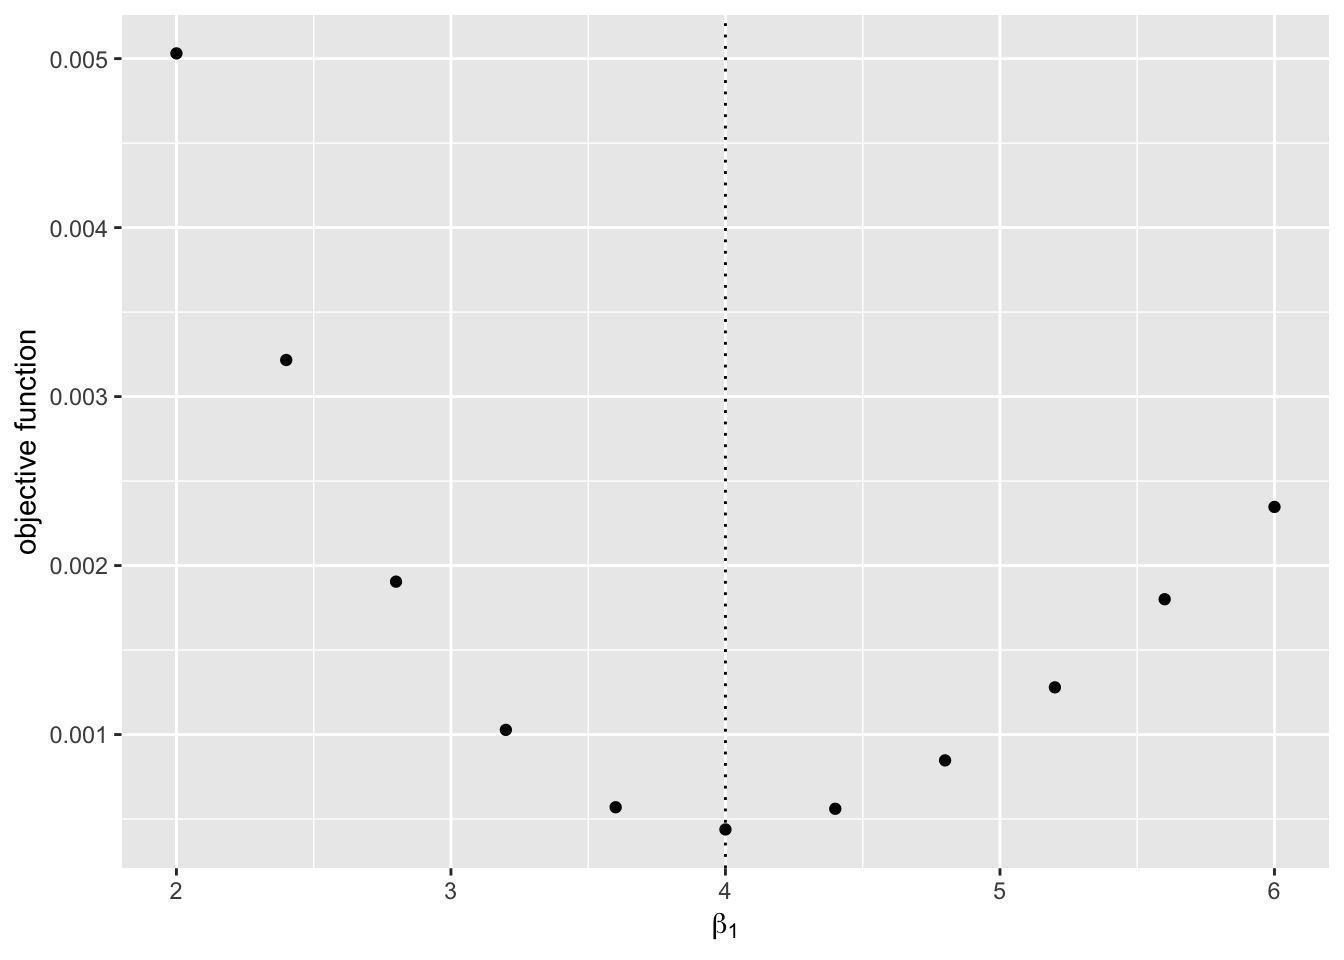
\includegraphics{lecture_files/figure-latex/unnamed-chunk-34-1} \end{center}

\begin{enumerate}
\def\labelenumi{\arabic{enumi}.}
\tightlist
\item
  Find and report \(\beta\) that maximizes the log likelihood for the
  simulated data. You can use \texttt{optim} function to achieve this.
  You will use \texttt{Brent} method and set the lower bound at -1 and
  upper bound at 1 for the parameter search.
\end{enumerate}

\begin{verbatim}
## $par
## [1] 0.2371046
## 
## $value
## [1] -0.6861689
## 
## $counts
## function gradient 
##       NA       NA 
## 
## $convergence
## [1] 0
## 
## $message
## NULL
\end{verbatim}

\chapter{Assignment 2: Production Function
Estimation}\label{assignment2}

The deadline is \textbf{February 28 1:30pm}.

\section{Simulate data}\label{simulate-data-1}

Consider the following production and investment process for
\(j = 1, \cdots, 1000\) firms across \(t = 1, \cdots, 10\) periods.

The log production function is of the form: \[
y_{jt} = \beta_0 + \beta_l l_{jt} + \beta_k k_{jt} + \omega_{jt} + \eta_{jt},
\] where \(\omega_{jt}\) is an anticipated shock and \(\eta_{jt}\) is an
ex post shock.

The anticipated shocks evolve as: \[
\omega_{jt} = \alpha \omega_{j, t - 1} + \nu_{jt},
\] where \(\nu_{jt}\) is an i.i.d. normal random variable with mean 0
and standard deviation \(\sigma_\nu\). The ex post shock is an i.i.d.
normal random variable with mean 0 and standard deviation
\(\sigma_{\eta}\).

The product price the same across firms and normalized at 1. The price
is normalized at 1. The wage \(w_t\) is constant at 0.5.

Finally, the capital accumulate according to: \[
K_{j, t + 1} = (1 - \delta) K_{jt} + I_{jt}.
\]

We set the parameters as follows:

\begin{longtable}[]{@{}lll@{}}
\toprule
parameter & variable & value\tabularnewline
\midrule
\endhead
\(\beta_0\) & \texttt{beta\_0} & 1\tabularnewline
\(\beta_l\) & \texttt{beta\_l} & 0.2\tabularnewline
\(\beta_k\) & \texttt{beta\_k} & 0.7\tabularnewline
\(\alpha\) & \texttt{alpha} & 0.7\tabularnewline
\(\sigma_{\eta}\) & \texttt{sigma\_eta} & 0.2\tabularnewline
\(\sigma_{\nu}\) & \texttt{sigma\_nu} & 0.5\tabularnewline
\(\sigma_{w}\) & \texttt{sigma\_w} & 0.1\tabularnewline
\(\delta\) & \texttt{delta} & 0.05\tabularnewline
\bottomrule
\end{longtable}

\begin{enumerate}
\def\labelenumi{\arabic{enumi}.}
\item
  Define the parameter variables as above.
\item
  Write a function that returns the log output given \(l_{jt}\),
  \(k_{jt}\), \(\omega_{jt}\), and \(\eta_{jt}\) under the given
  parameter values according to the above production function and name
  it
  \texttt{log\_production(l,\ k,\ omega,\ eta,\ beta\_0,\ beta\_l,\ beta\_k)}.
\end{enumerate}

Suppose that the labor is determined after \(\omega_{jt}\) is observed,
but before \(\eta_{jt}\) is observed, given the log capital level
\(k_{jt}\).

\begin{enumerate}
\def\labelenumi{\arabic{enumi}.}
\setcounter{enumi}{2}
\tightlist
\item
  Derive the optimal log labor as a function of \(\omega_{jt}\),
  \(\eta_{jt}\), \(k_{jt}\), and wage. Write a function to return the
  optimal log labor given the variables and parameters and name it
  \texttt{log\_labor\_choice(k,\ wage,\ omega,\ beta\_0,\ beta\_l,\ beta\_k,\ sigma\_eta)}.
\end{enumerate}

As discussed in the class, if there is no additional variation in labor,
the coefficient on the labor \(\beta_l\) is not identified. Thus, if we
generate labor choice from the previous function, \(\beta_l\) will not
be identified from the simulated data. To see this, we write a modified
version of the previous function in which \(\omega_{jt}\) is replaced
with \(\omega_{jt} + \iota_{jt}\), where \(\iota_{jt}\) is an
optimization error that follows an i.i.d. normal distribution with mean
0 and standard deviation 0.05. That is, the manager of the firm
perceives as if the shock is \(\omega_{jt} + \iota_{jt}\), even though
the true shock is \(\omega_{jt}\).

\begin{enumerate}
\def\labelenumi{\arabic{enumi}.}
\setcounter{enumi}{3}
\tightlist
\item
  Modify the previous function by including \(\iota_{jt}\) as an
  additional input and name it
  \texttt{log\_labor\_choice\_error(k,\ wage,\ omega,\ beta\_0,\ beta\_l,\ beta\_k,\ iota,\ sigma\_eta)}.
\end{enumerate}

Consider an investment process such that: \[
I_{jt} = (\delta + \gamma \omega_{jt}) K_{jt},
\] where \(I_{jt}\) and \(K_{jt}\) are investment and capital in level.
Set \(\gamma = 0.1\), i.e., the investment is strictly increasing in
\(\omega_{jt}\). The investment function should be derived by solving
the dynamic problem of a firm. But here, we just specify it in a
reduced-form.

\begin{enumerate}
\def\labelenumi{\arabic{enumi}.}
\setcounter{enumi}{4}
\tightlist
\item
  Define variable \(\gamma\) and assign it the value. Write a function
  that returns the investment given \(K_{jt}\), \(\omega_{jt}\), and
  parameter values, according to the previous equation, and name it
  \texttt{investment\_choice(k,\ omega,\ gamma,\ delta)}.
\end{enumerate}

Simulate the data first using the labor choice without optimization
error and second using the labor choice with optimization error. To do
so, we specify the initial values for the state variables \(k_{jt}\) and
\(\omega_{jt}\) as follows.

\begin{enumerate}
\def\labelenumi{\arabic{enumi}.}
\setcounter{enumi}{5}
\tightlist
\item
  Draw \(k_{j1}\) from an i.i.d. normal distribution with mean 1 and
  standard deviation 0.5. Draw \(\omega_{j1}\) from its stationary
  distribution (check the stationary distribution of AR(1) process).
  Draw a wage. Before simulating the rest of the data, set the seed at
  1.
\end{enumerate}

\begin{verbatim}
## # A tibble: 1,000 x 5
##        j     t     k   omega  wage
##    <int> <dbl> <dbl>   <dbl> <dbl>
##  1     1     1 0.687  0.795    0.5
##  2     2     1 1.09   0.779    0.5
##  3     3     1 0.582 -0.610    0.5
##  4     4     1 1.80   0.148    0.5
##  5     5     1 1.16   0.0486   0.5
##  6     6     1 0.590 -1.16     0.5
##  7     7     1 1.24   0.568    0.5
##  8     8     1 1.37  -1.34     0.5
##  9     9     1 1.29  -0.873    0.5
## 10    10     1 0.847  0.699    0.5
## # ... with 990 more rows
\end{verbatim}

\begin{enumerate}
\def\labelenumi{\arabic{enumi}.}
\setcounter{enumi}{6}
\tightlist
\item
  Draw optimization error \(\iota_{jt}\) and compute the labor and
  investment choice of period 1. For labor choice, compute both types of
  labor choices.
\end{enumerate}

\begin{verbatim}
## # A tibble: 1,000 x 9
##        j     t     k   omega  wage     iota      l l_error       I
##    <int> <dbl> <dbl>   <dbl> <dbl>    <dbl>  <dbl>   <dbl>   <dbl>
##  1     1     1 0.687  0.795    0.5 -0.0443   1.72   1.67    0.257 
##  2     2     1 1.09   0.779    0.5 -0.0961   2.06   1.94    0.381 
##  3     3     1 0.582 -0.610    0.5  0.0810  -0.123 -0.0218 -0.0196
##  4     4     1 1.80   0.148    0.5  0.0260   1.89   1.92    0.391 
##  5     5     1 1.16   0.0486   0.5 -0.00279  1.21   1.21    0.176 
##  6     6     1 0.590 -1.16     0.5  0.0348  -0.809 -0.766  -0.120 
##  7     7     1 1.24   0.568    0.5  0.00268  1.93   1.93    0.370 
##  8     8     1 1.37  -1.34     0.5 -0.0655  -0.346 -0.428  -0.330 
##  9     9     1 1.29  -0.873    0.5 -0.106    0.165  0.0327 -0.135 
## 10    10     1 0.847  0.699    0.5 -0.0104   1.74   1.73    0.280 
## # ... with 990 more rows
\end{verbatim}

\begin{enumerate}
\def\labelenumi{\arabic{enumi}.}
\setcounter{enumi}{7}
\tightlist
\item
  Draw ex post shock and compute the output according to the production
  function for both labor without optimization error and with
  optimization error. Name the output without optimization error
  \texttt{y} and the one with optimization error \texttt{y\_error}.
\end{enumerate}

\begin{verbatim}
## # A tibble: 1,000 x 12
##        j     t     k   omega  wage     iota      l l_error       I     eta
##    <int> <dbl> <dbl>   <dbl> <dbl>    <dbl>  <dbl>   <dbl>   <dbl>   <dbl>
##  1     1     1 0.687  0.795    0.5 -0.0443   1.72   1.67    0.257   0.148 
##  2     2     1 1.09   0.779    0.5 -0.0961   2.06   1.94    0.381   0.0773
##  3     3     1 0.582 -0.610    0.5  0.0810  -0.123 -0.0218 -0.0196  0.259 
##  4     4     1 1.80   0.148    0.5  0.0260   1.89   1.92    0.391  -0.161 
##  5     5     1 1.16   0.0486   0.5 -0.00279  1.21   1.21    0.176  -0.321 
##  6     6     1 0.590 -1.16     0.5  0.0348  -0.809 -0.766  -0.120   0.187 
##  7     7     1 1.24   0.568    0.5  0.00268  1.93   1.93    0.370   0.361 
##  8     8     1 1.37  -1.34     0.5 -0.0655  -0.346 -0.428  -0.330  -0.0113
##  9     9     1 1.29  -0.873    0.5 -0.106    0.165  0.0327 -0.135   0.377 
## 10    10     1 0.847  0.699    0.5 -0.0104   1.74   1.73    0.280   0.316 
## # ... with 990 more rows, and 2 more variables: y <dbl>, y_error <dbl>
\end{verbatim}

\begin{enumerate}
\def\labelenumi{\arabic{enumi}.}
\setcounter{enumi}{8}
\tightlist
\item
  Repeat this procedure for \(t = 1, \cdots 10\) by updating the capital
  and anticipated shocks, and name the resulting data frame
  \texttt{df\_T}.
\end{enumerate}

\begin{verbatim}
## # A tibble: 10,000 x 13
##        j     t     k   omega  wage     iota      l l_error       I     eta
##    <int> <dbl> <dbl>   <dbl> <dbl>    <dbl>  <dbl>   <dbl>   <dbl>   <dbl>
##  1     1     1 0.687  0.795    0.5 -0.0443   1.72   1.67    0.257   0.148 
##  2     2     1 1.09   0.779    0.5 -0.0961   2.06   1.94    0.381   0.0773
##  3     3     1 0.582 -0.610    0.5  0.0810  -0.123 -0.0218 -0.0196  0.259 
##  4     4     1 1.80   0.148    0.5  0.0260   1.89   1.92    0.391  -0.161 
##  5     5     1 1.16   0.0486   0.5 -0.00279  1.21   1.21    0.176  -0.321 
##  6     6     1 0.590 -1.16     0.5  0.0348  -0.809 -0.766  -0.120   0.187 
##  7     7     1 1.24   0.568    0.5  0.00268  1.93   1.93    0.370   0.361 
##  8     8     1 1.37  -1.34     0.5 -0.0655  -0.346 -0.428  -0.330  -0.0113
##  9     9     1 1.29  -0.873    0.5 -0.106    0.165  0.0327 -0.135   0.377 
## 10    10     1 0.847  0.699    0.5 -0.0104   1.74   1.73    0.280   0.316 
## # ... with 9,990 more rows, and 3 more variables: y <dbl>, y_error <dbl>,
## #   nu <dbl>
\end{verbatim}

\begin{enumerate}
\def\labelenumi{\arabic{enumi}.}
\setcounter{enumi}{9}
\tightlist
\item
  Check the simulated data by making summary table.
\end{enumerate}

\begin{tabular}{l|r|r|r|r|r}
\hline
  & N & Mean & Sd & Min & Max\\
\hline
j & 10000 & 500.5000000 & 288.6894251 & 1.0000000 & 1000.0000000\\
\hline
t & 10000 & 5.5000000 & 2.8724249 & 1.0000000 & 10.0000000\\
\hline
k & 10000 & 0.9797900 & 0.5838949 & -1.2822534 & 3.2332312\\
\hline
omega & 10000 & -0.0055826 & 0.7025102 & -2.5894171 & 2.6281307\\
\hline
wage & 10000 & 0.5000000 & 0.0000000 & 0.5000000 & 0.5000000\\
\hline
iota & 10000 & -0.0000696 & 0.0502883 & -0.1841453 & 0.1715419\\
\hline
l & 10000 & 0.9799746 & 1.0965108 & -3.3281023 & 4.9679634\\
\hline
l\_error & 10000 & 0.9798876 & 1.0971595 & -3.3765433 & 4.9520674\\
\hline
I & 10000 & 0.1793502 & 0.3006526 & -1.2722627 & 3.2975332\\
\hline
eta & 10000 & 0.0015825 & 0.2001539 & -0.7650371 & 0.7455922\\
\hline
y & 10000 & 1.8778479 & 1.1171035 & -2.4680251 & 6.1228291\\
\hline
y\_error & 10000 & 1.8778305 & 1.1169266 & -2.4777133 & 6.1196499\\
\hline
nu & 10000 & -0.0021155 & 0.4984324 & -2.1513907 & 1.8253882\\
\hline
\end{tabular}

\section{Estimate the parameters}\label{estimate-the-parameters}

For now, use the labor choice with optimization error.

\begin{enumerate}
\def\labelenumi{\arabic{enumi}.}
\tightlist
\item
  First, simply regress \(y_{jt}\) on \(l_{jt}\) and \(k_{jt}\) using
  the least square method. This is likely to give an upwardly biased
  estimates on \(\beta_l\) and \(\beta_k\). Why is it?
\end{enumerate}

\begin{verbatim}
## 
## Call:
## lm(formula = y_error ~ l_error + k, data = df_T)
## 
## Residuals:
##      Min       1Q   Median       3Q      Max 
## -0.73002 -0.14117 -0.00071  0.13743  0.87983 
## 
## Coefficients:
##             Estimate Std. Error t value Pr(>|t|)    
## (Intercept) 0.892542   0.004058 219.966   <2e-16 ***
## l_error     0.997913   0.002396 416.454   <2e-16 ***
## k           0.007599   0.004503   1.688   0.0915 .  
## ---
## Signif. codes:  0 '***' 0.001 '**' 0.01 '*' 0.05 '.' 0.1 ' ' 1
## 
## Residual standard error: 0.2068 on 9997 degrees of freedom
## Multiple R-squared:  0.9657, Adjusted R-squared:  0.9657 
## F-statistic: 1.408e+05 on 2 and 9997 DF,  p-value: < 2.2e-16
\end{verbatim}

\begin{enumerate}
\def\labelenumi{\arabic{enumi}.}
\setcounter{enumi}{1}
\tightlist
\item
  Second, take within-transformation on \(y_{jt}\), \(l_{jt}\), and
  \(k_{jt}\) and let \(\Delta y_{jt}\), \(\Delta l_{jt}\), and
  \(\Delta k_{jt}\) denote them. Then, regress \(\Delta y_{jt}\) on
  \(\Delta l_{jt}\), and \(\Delta k_{jt}\) by the least squares method.
\end{enumerate}

\begin{verbatim}
## 
## Call:
## lm(formula = dy_error ~ -1 + dl_error + dk, data = df_T_within)
## 
## Residuals:
##      Min       1Q   Median       3Q      Max 
## -0.72450 -0.13285 -0.00244  0.12931  0.77657 
## 
## Coefficients:
##            Estimate Std. Error t value Pr(>|t|)    
## dl_error  0.9910916  0.0029548 335.413   <2e-16 ***
## dk       -0.0009029  0.0127539  -0.071    0.944    
## ---
## Signif. codes:  0 '***' 0.001 '**' 0.01 '*' 0.05 '.' 0.1 ' ' 1
## 
## Residual standard error: 0.1961 on 9998 degrees of freedom
## Multiple R-squared:  0.9184, Adjusted R-squared:  0.9184 
## F-statistic: 5.629e+04 on 2 and 9998 DF,  p-value: < 2.2e-16
\end{verbatim}

Next, we attempt to estimate the parameters using Olley-Pakes method.
Estimate the first-step model of Olley-Pakes method: \[
y_{jt} = \beta_0 + \beta_1 l_{jt} + \phi(k_{jt}, I_{jt}) + \eta_{jt},
\] by approximating \(\phi_t\) by a kernel function.

Remark that \(\phi\) in general depends on observed and unobserved state
variables. For this reason, in theory, \(\phi\) should be estimated for
each period. In this exercise, we assume \(\phi\) is common across
periods because we know that there is no unobserved state variables in
the true data generating process. Moreover, we do not include \(w_t\)
because we know that it is time -invariant. Do not forget to consider
them in the actual data analysis.

You can use \texttt{npplreg} function of \texttt{np} package to estimate
a partially linear model with a multivariate kernel. You first use
\texttt{npplregbw} to obtain the optimal band width and then use
\texttt{npplreg} to estimate the model under the optimal bandwidth. The
computation of the optimal bandwidth is time consuming.

\begin{enumerate}
\def\labelenumi{\arabic{enumi}.}
\setcounter{enumi}{2}
\tightlist
\item
  Return the summary of the first stage estimation and plot the fitted
  values against the data points.
\end{enumerate}

\begin{verbatim}
## 
## Partially Linear Model
## Regression data: 10000 training points, in 5 variable(s)
## With 3 linear parametric regressor(s), 2 nonparametric regressor(s)
## 
##                     y(z)           
## Bandwidth(s): 0.07355058 0.01435558
## 
##                     x(z)           
## Bandwidth(s): 0.03908594 0.01191551
##               0.01397428 3.74952954
##               0.83529394 0.00398329
## 
##                   l_error        k        I
## Coefficient(s): 0.2485295 2.355522 5.345144
## 
## Kernel Regression Estimator: Local-Constant
## Bandwidth Type: Fixed
## 
## Residual standard error: 0.1934585
## R-squared: 0.970064
## 
## Continuous Kernel Type: Second-Order Gaussian
## No. Continuous Explanatory Vars.: 2
\end{verbatim}

\begin{center}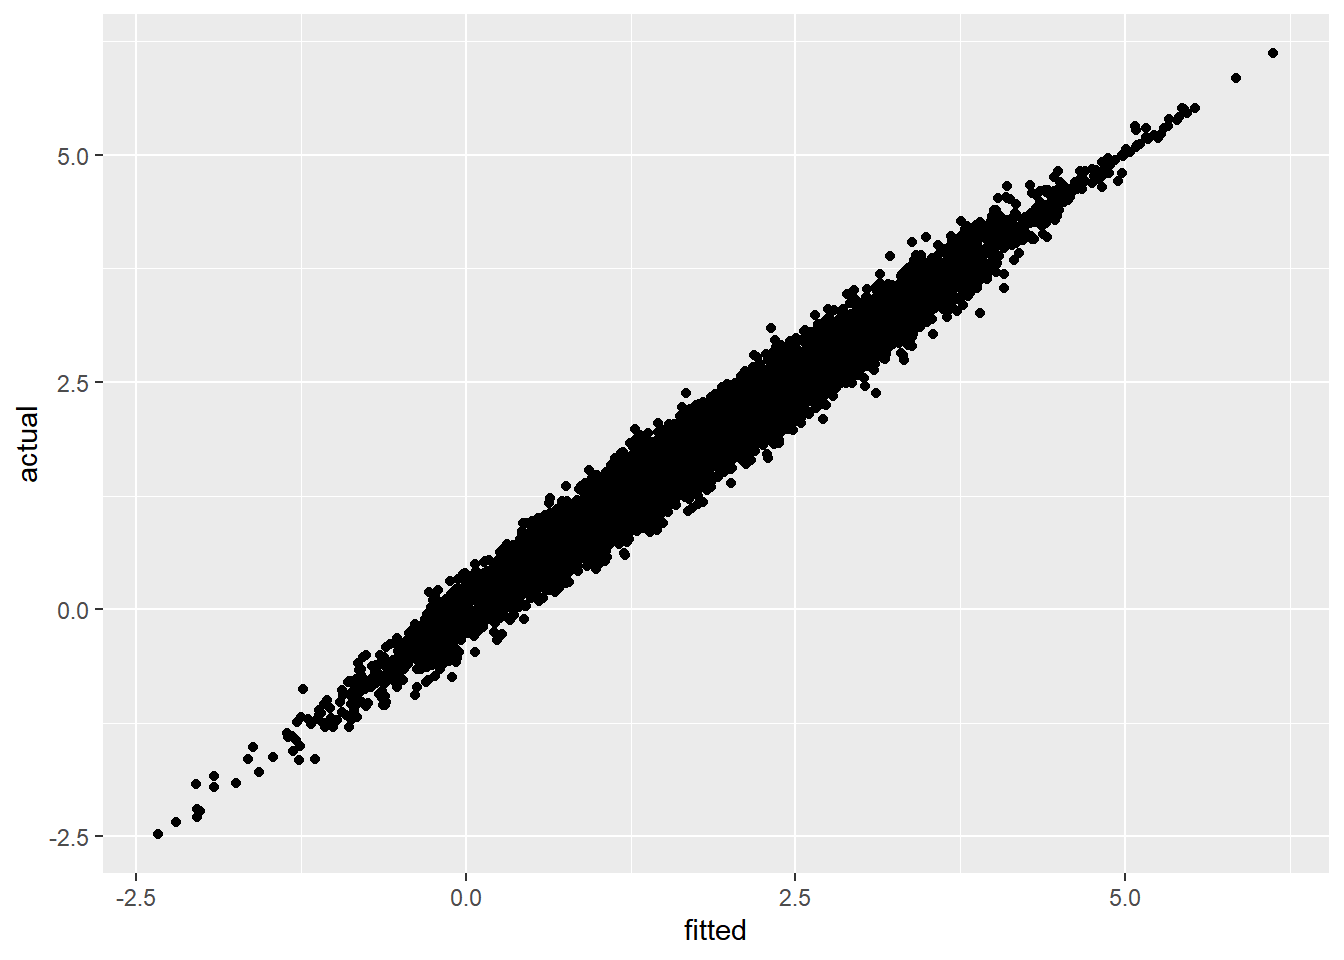
\includegraphics{lecture_files/figure-latex/unnamed-chunk-51-1} \end{center}

\begin{enumerate}
\def\labelenumi{\arabic{enumi}.}
\setcounter{enumi}{3}
\tightlist
\item
  Check that \(\beta_l\) is not identified with the data without
  optimization error. Estimate the first stage model of Olley-Pakes with
  the labor choice without optimization error and report the result.
\end{enumerate}

\begin{verbatim}
## 
## Partially Linear Model
## Regression data: 10000 training points, in 5 variable(s)
## With 3 linear parametric regressor(s), 2 nonparametric regressor(s)
## 
##                     y(z)           
## Bandwidth(s): 0.07347226 0.01437256
## 
##                     x(z)            
## Bandwidth(s): 0.02960021 0.009986945
##               0.01397428 3.749529542
##               0.83529394 0.003983290
## 
##                        l        k         I
## Coefficient(s): 1.180628 2.034182 0.7805077
## 
## Kernel Regression Estimator: Local-Constant
## Bandwidth Type: Fixed
## 
## Residual standard error: 0.1932285
## R-squared: 0.970116
## 
## Continuous Kernel Type: Second-Order Gaussian
## No. Continuous Explanatory Vars.: 2
\end{verbatim}

Then, we estimate the second stage model of Olley-Pakes method: \[
y_{jt} - \hat{\beta_l} l_{jt} = \beta_0 + \beta_k k_{jt} + \alpha[\hat{\phi}(k_{j, t - 1}, I_{j, t - 1}) - \beta_0 - \beta_k k_{jt}] + \nu_{jt} + \eta_{jt}.
\]

In this model, we do not have to non-parametetrically estimate the
conditional expectation of \(\omega_{jt}\) on \(\omega_{j, t - 1}\),
because we know that the anticipated shock follows an AR(1) process.
Remark that we in general have to non-parametrically estimate it.

The model is non-linear in parameters, because of the term
\(\alpha \beta_0\) and \(\alpha \beta_k\). We estimate \(\alpha\),
\(\beta_0\), and \(\beta_k\) by a GMM estimator. The moment is: \[
g_{JT}(\alpha, \beta_0, \beta_k) \equiv \frac{1}{JT}\sum_{j = 1}^J \sum_{t = 1}^T \{y_{jt} - \hat{\beta_l} l_{jt} - \beta_0 - \beta_k k_{jt} - \alpha[\hat{\phi}(k_{j, t - 1}, I_{j, t - 1}) - \beta_0 - \beta_k k_{jt}]\} 
\begin{bmatrix}
k_{jt} \\
k_{j, t - 1} \\
I_{j, t - 1}
\end{bmatrix}.
\]

\begin{enumerate}
\def\labelenumi{\arabic{enumi}.}
\setcounter{enumi}{4}
\tightlist
\item
  Using the estimates in the first step, compute: \[
  y_{jt} - \hat{\beta_l} l_{jt},
  \] and: \[
  \hat{\phi}(k_{j, t - 1}, I_{j, t - 1}),
  \] for each \(j\) and \(t\) and save it as a data frame names
  \texttt{df\_T\_1st}.
\end{enumerate}

\begin{verbatim}
## # A tibble: 10,000 x 4
##        j     t y_error_tilde phi_t_1
##    <int> <dbl>         <dbl>   <dbl>
##  1     1     1         2.34   NA    
##  2     1     2         1.37    2.21 
##  3     1     3         0.621   1.49 
##  4     1     4         0.447   0.882
##  5     1     5         0.878   0.611
##  6     1     6         1.62    0.926
##  7     1     7         0.558   1.40 
##  8     1     8         0.684   0.439
##  9     1     9         0.939   0.520
## 10     1    10         1.49    0.836
## # ... with 9,990 more rows
\end{verbatim}

\begin{enumerate}
\def\labelenumi{\arabic{enumi}.}
\setcounter{enumi}{5}
\tightlist
\item
  Compute a function that returns the value of
  \(g_{JT}(\alpha, \beta_0, \beta_k)\) given parameter values, data, and
  \texttt{df\_T\_1st}, and name it \texttt{moment\_OP\_2nd}. Show the
  values of the moments evaluated at the true parameters.
\end{enumerate}

\begin{verbatim}
## [1] -0.018507303 -0.019038229 -0.003867714
\end{verbatim}

Based on the moment, we can define the objective function of a
generalized method of moments estimator with a weighting matrix \(W\)
as: \[
Q_{JT}(\alpha, \beta_0, \beta_k) \equiv g_{JT}(\alpha, \beta_0, \beta_k)' W g_{JT}(\alpha, \beta_0, \beta_k).
\]

\begin{enumerate}
\def\labelenumi{\arabic{enumi}.}
\setcounter{enumi}{6}
\tightlist
\item
  Write a function that returns the value of
  \(Q_{JT}(\alpha, \beta_0, \beta_k)\) given the vector of parameter
  values, data, and \texttt{df\_T\_1st}, and name it
  \texttt{objective\_OP\_2nd}. Setting \(W\) at the identity matrix,
  show the value of the objective function evaluated at the true
  parameters.
\end{enumerate}

\begin{verbatim}
##              [,1]
## [1,] 0.0007199336
\end{verbatim}

\begin{enumerate}
\def\labelenumi{\arabic{enumi}.}
\setcounter{enumi}{7}
\tightlist
\item
  Draw the graph of the objective function when one of \(\alpha\),
  \(\beta_0\), and \(\beta_k\) are changed from 0 to 1 by 0.1 while the
  others are set at the true value. Is the objective function minimized
  at around the true value?
\end{enumerate}

\begin{center}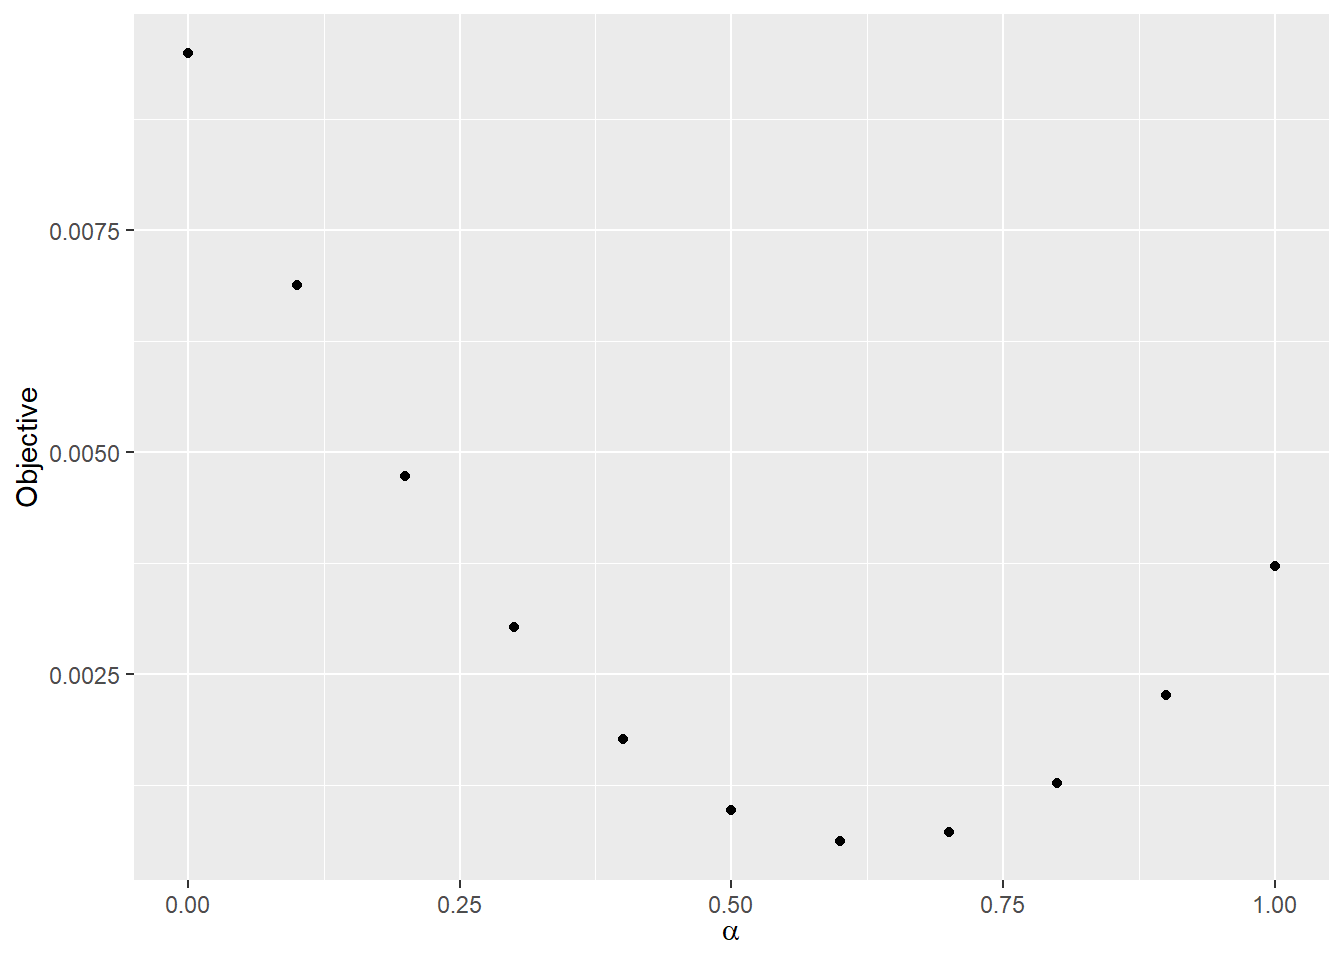
\includegraphics{lecture_files/figure-latex/unnamed-chunk-58-1} \end{center}

\begin{center}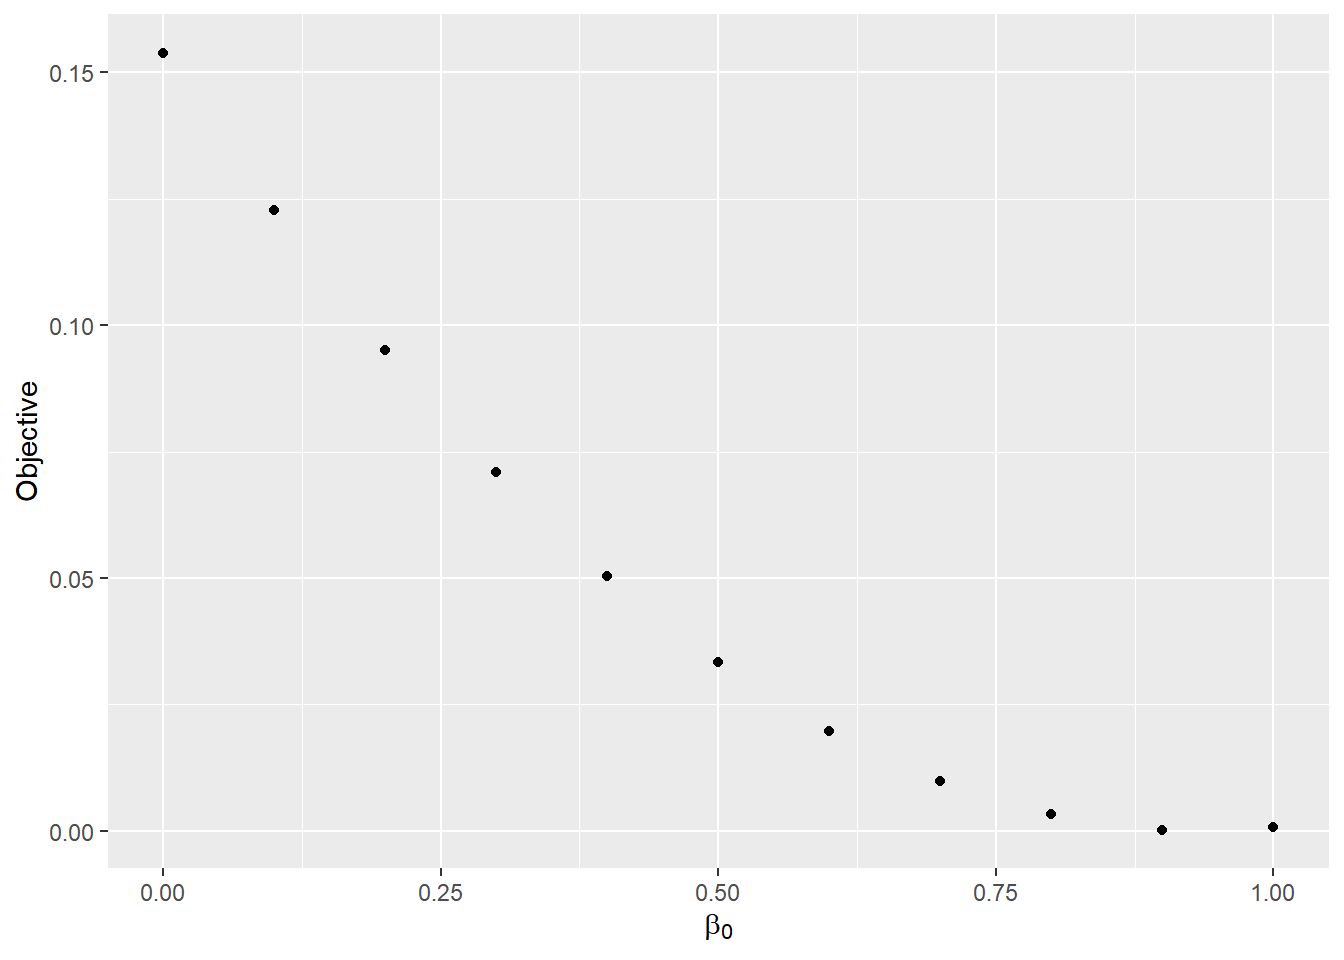
\includegraphics{lecture_files/figure-latex/unnamed-chunk-58-2} \end{center}

\begin{center}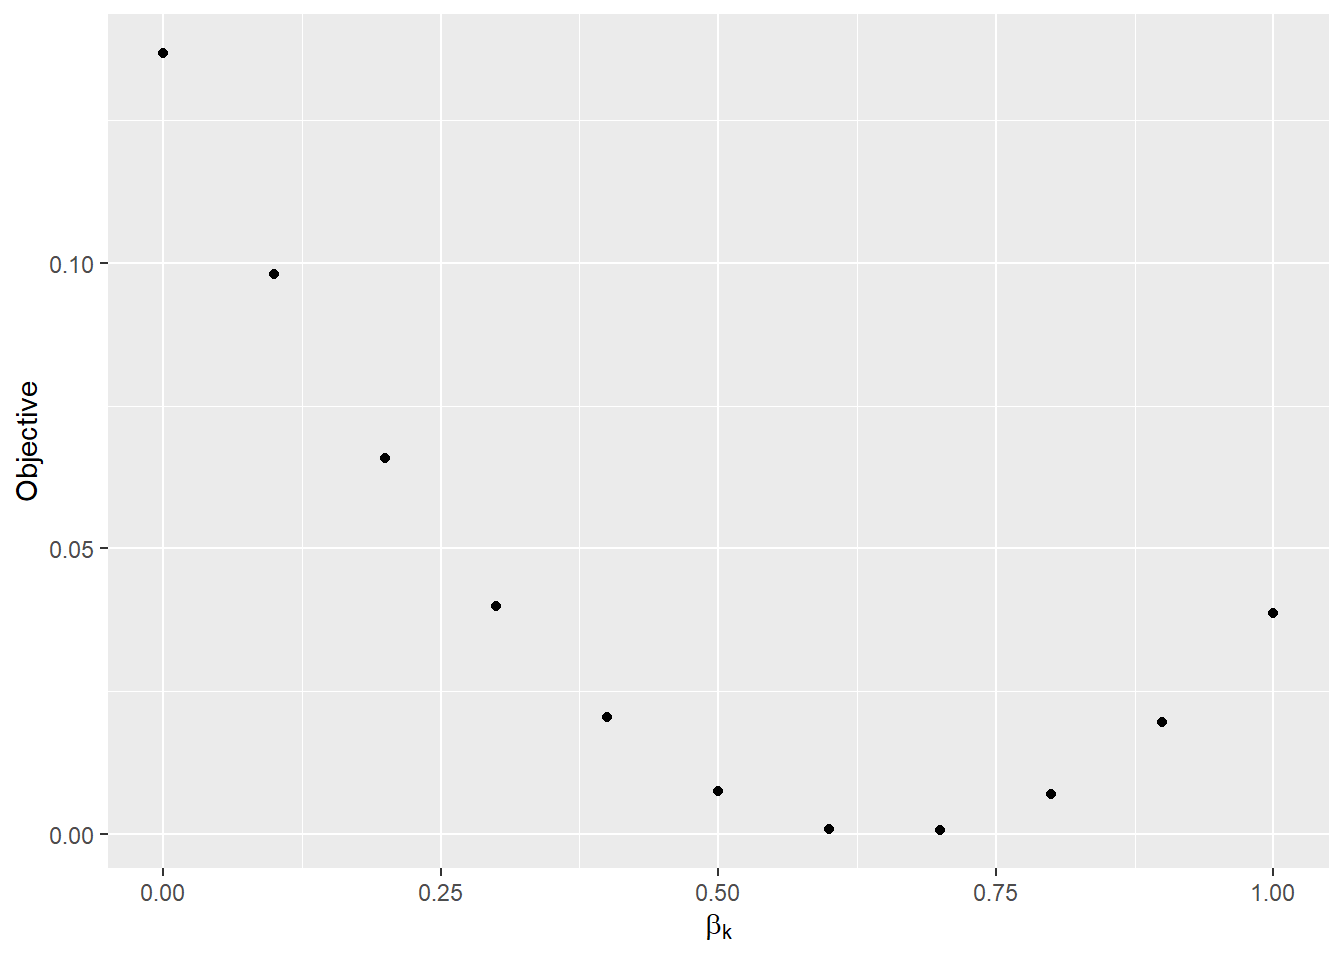
\includegraphics{lecture_files/figure-latex/unnamed-chunk-58-3} \end{center}

\begin{enumerate}
\def\labelenumi{\arabic{enumi}.}
\setcounter{enumi}{8}
\tightlist
\item
  Find the parameters that minimize the objective function using
  \texttt{optim}. You may use \texttt{L-BFGS-B} method to solve it.
\end{enumerate}

\begin{verbatim}
## $par
## [1] 0.7020260 0.9766308 0.6693945
## 
## $value
## [1] 1.994601e-07
## 
## $counts
## function gradient 
##       10       10 
## 
## $convergence
## [1] 0
## 
## $message
## [1] "CONVERGENCE: REL_REDUCTION_OF_F <= FACTR*EPSMCH"
\end{verbatim}

\chapter{Assignment 3: Demand Function Estimation I}\label{assignment3}

The deadline is \textbf{March 11 1:30pm}.

\section{Simulate data}\label{simulate-data-2}

We simulate data from a discrete choice model. There are \(T\) markets
and each market has \(N\) consumers. There are \(J\) products and the
indirect utility of consumer \(i\) in market \(t\) for product \(j\) is:
\[
u_{itj} = \beta_{it}' x_j + \alpha_{it} p_{jt} + \xi_{jt} + \epsilon_{ijt},
\] where \(\epsilon_{ijt}\) is an i.i.d. type-I extreme random variable.
\(x_j\) is \(K\)-dimensional observed characteristics of the product.
\(p_{jt}\) is the retail price of the product in the market.

\(\xi_{jt}\) is product-market specific fixed effect. \(p_{jt}\) can be
correlated with \(\xi_{jt}\) but \(x_{jt}\)s are independent of
\(\xi_{jt}\). \(j = 0\) is an outside option whose indirect utility is:
\[
u_{it0} = \epsilon_{i0t},
\] where \(\epsilon_{i0t}\) is an i.i.d. type-I extreme random variable.

\(\beta_{it}\) and \(\alpha_{it}\) are different across consumers, and
they are distributed as: \[
\beta_{itk} = \beta_{0k} + \sigma_k \nu_{itk},
\] \[
\alpha_{it} = - \exp(\mu + \omega \upsilon_{it}) = - \exp(\mu + \frac{\omega^2}{2}) + [- \exp(\mu + \omega \upsilon_{it}) + \exp(\mu + \frac{\omega^2}{2})] \equiv \alpha_0 + \tilde{\alpha}_{it},
\] where \(\nu_{itk}\) for \(k = 1, \cdots, K\) and \(\upsilon_{it}\)
are i.i.d. standard normal random variables. \(\alpha_0\) is the mean of
\(\alpha_i\) and \(\tilde{\alpha}_i\) is the deviation from the mean.

Given a choice set in the market, \(\mathcal{J}_t \cup \{0\}\), a
consumer chooses the alternative that maximizes her utility: \[
q_{ijt} = 1\{u_{ijt} = \max_{k \in \mathcal{J}_t \cup \{0\}} u_{ikt}\}.
\] The choice probability of product \(j\) for consumer \(i\) in market
\(t\) is: \[
\sigma_{jt}(p_t, x_t, \xi_t) = \mathbb{P}\{u_{ijt} = \max_{k \in \mathcal{J}_t \cup \{0\}} u_{ikt}\}.
\]

Suppose that we only observe the share data: \[
s_{jt} = \frac{1}{N} \sum_{i = 1}^N q_{ijt},
\] along with the product-market characteristics \(x_{jt}\) and the
retail prices \(p_{jt}\) for \(j \in \mathcal{J}_t \cup \{0\}\) for
\(t = 1, \cdots, T\). We do not observe the choice data \(q_{ijt}\) nor
shocks \(\xi_{jt}, \nu_{it}, \upsilon_{it}, \epsilon_{ijt}\).

In this assignment, we consider a model with \(\xi_{jt} = 0\), i.e., the
model without the unobserved fixed effects. However, the code to
simulate data should be written for general \(\xi_{jt}\), so that we can
use the same code in the next assignment in which we consider a model
with the unobserved fixed effects.

\begin{enumerate}
\def\labelenumi{\arabic{enumi}.}
\tightlist
\item
  Set the seed, constants, and parameters of interest as follows.
\end{enumerate}

\begin{Shaded}
\begin{Highlighting}[]
\CommentTok{# set the seed}
\KeywordTok{set.seed}\NormalTok{(}\DecValTok{1}\NormalTok{)}
\CommentTok{# number of products}
\NormalTok{J <-}\StringTok{ }\DecValTok{10}
\CommentTok{# dimension of product characteristics including the intercept}
\NormalTok{K <-}\StringTok{ }\DecValTok{3}
\CommentTok{# number of markets}
\NormalTok{T <-}\StringTok{ }\DecValTok{100}
\CommentTok{# number of consumers per market}
\NormalTok{N <-}\StringTok{ }\DecValTok{500}
\CommentTok{# number of Monte Carlo}
\NormalTok{L <-}\StringTok{ }\DecValTok{500}
\end{Highlighting}
\end{Shaded}

\begin{Shaded}
\begin{Highlighting}[]
\CommentTok{# set parameters of interests}
\NormalTok{beta <-}\StringTok{ }\KeywordTok{rnorm}\NormalTok{(K); }
\NormalTok{beta[}\DecValTok{1}\NormalTok{] <-}\StringTok{ }\DecValTok{4}
\NormalTok{beta}
\end{Highlighting}
\end{Shaded}

\begin{verbatim}
## [1]  4.0000000  0.1836433 -0.8356286
\end{verbatim}

\begin{Shaded}
\begin{Highlighting}[]
\NormalTok{sigma <-}\StringTok{ }\KeywordTok{abs}\NormalTok{(}\KeywordTok{rnorm}\NormalTok{(K)); sigma}
\end{Highlighting}
\end{Shaded}

\begin{verbatim}
## [1] 1.5952808 0.3295078 0.8204684
\end{verbatim}

\begin{Shaded}
\begin{Highlighting}[]
\NormalTok{mu <-}\StringTok{ }\FloatTok{0.5}
\NormalTok{omega <-}\StringTok{ }\DecValTok{1}
\end{Highlighting}
\end{Shaded}

Generate the covariates as follows.

The product-market characteristics: \[
x_{j1} = 1, x_{jk} \sim N(0, \sigma_x), k = 2, \cdots, K,
\] where \(\sigma_x\) is referred to as \texttt{sd\_x} in the code.

The product-market-specific unobserved fixed effect: \[
\xi_{jt} = 0.
\] The marginal cost of product \(j\) in market \(t\): \[
c_{jt} \sim \text{logNormal}(0, \sigma_c),
\] where \(\sigma_c\) is referred to as \texttt{sd\_c} in the code.

The retail price: \[
p_{jt} - c_{jt} \sim \text{logNorm}(\gamma \xi_{jt}, \sigma_p),
\] where \(\gamma\) is referred to as \texttt{price\_xi} and
\(\sigma_p\) as \texttt{sd\_p} in the code. This price is not the
equilibrium price. We will revisit this point in a subsequent
assignment.

The value of the auxiliary parameters are set as follows:

\begin{Shaded}
\begin{Highlighting}[]
\CommentTok{# set auxiliary parameters}
\NormalTok{price_xi <-}\StringTok{ }\DecValTok{1}
\NormalTok{prop_jt <-}\StringTok{ }\FloatTok{0.6}
\NormalTok{sd_x <-}\StringTok{ }\FloatTok{0.5}
\NormalTok{sd_c <-}\StringTok{ }\FloatTok{0.05}
\NormalTok{sd_p <-}\StringTok{ }\FloatTok{0.05}
\end{Highlighting}
\end{Shaded}

\begin{enumerate}
\def\labelenumi{\arabic{enumi}.}
\setcounter{enumi}{1}
\tightlist
\item
  \texttt{X} is the data frame such that a row contains the
  characteristics vector \(x_{j}\) of a product and columns are product
  index and observed product characteristics. The dimension of the
  characteristics \(K\) is specified above. Add the row of the outside
  option whose index is \(0\) and all the characteristics are zero.
\end{enumerate}

\begin{Shaded}
\begin{Highlighting}[]
\NormalTok{X}
\end{Highlighting}
\end{Shaded}

\begin{verbatim}
## # A tibble: 11 x 4
##        j   x_1     x_2      x_3
##    <dbl> <dbl>   <dbl>    <dbl>
##  1     0     0  0       0      
##  2     1     1  0.244  -0.00810
##  3     2     1  0.369   0.472  
##  4     3     1  0.288   0.411  
##  5     4     1 -0.153   0.297  
##  6     5     1  0.756   0.459  
##  7     6     1  0.195   0.391  
##  8     7     1 -0.311   0.0373 
##  9     8     1 -1.11   -0.995  
## 10     9     1  0.562   0.310  
## 11    10     1 -0.0225 -0.0281
\end{verbatim}

\begin{enumerate}
\def\labelenumi{\arabic{enumi}.}
\setcounter{enumi}{2}
\tightlist
\item
  \texttt{M} is the data frame such that a row contains the price
  \(\xi_{jt}\), marginal cost \(c_{jt}\), and price \(p_{jt}\). After
  generating the variables, drop \texttt{1\ -\ prop\_jt} products from
  each market using \texttt{dplyr::sample\_frac} function. The variation
  in the available products is important for the identification of the
  distribution of consumer-level unobserved heterogeneity. Add the row
  of the outside option to each market whose index is \(0\) and all the
  variables take value zero.
\end{enumerate}

\begin{Shaded}
\begin{Highlighting}[]
\NormalTok{M}
\end{Highlighting}
\end{Shaded}

\begin{verbatim}
## # A tibble: 700 x 5
##        j     t    xi     c     p
##    <dbl> <int> <dbl> <dbl> <dbl>
##  1     0     1     0 0      0   
##  2     1     1     0 0.951  1.93
##  3     5     1     0 0.974  1.94
##  4     6     1     0 0.980  1.96
##  5     7     1     0 0.961  1.94
##  6     8     1     0 0.989  1.99
##  7    10     1     0 1.02   2.09
##  8     0     2     0 0      0   
##  9     1     2     0 0.988  2.09
## 10     2     2     0 1.04   1.96
## # ... with 690 more rows
\end{verbatim}

\begin{enumerate}
\def\labelenumi{\arabic{enumi}.}
\setcounter{enumi}{3}
\tightlist
\item
  Generate the consumer-level heterogeneity. \texttt{V} is the data
  frame such that a row contains the vector of shocks to consumer-level
  heterogeneity, \((\nu_{i}', \upsilon_i)\). They are all i.i.d.
  standard normal random variables.
\end{enumerate}

\begin{Shaded}
\begin{Highlighting}[]
\NormalTok{V}
\end{Highlighting}
\end{Shaded}

\begin{verbatim}
## # A tibble: 50,000 x 6
##        i     t   v_x_1   v_x_2  v_x_3    v_p
##    <int> <int>   <dbl>   <dbl>  <dbl>  <dbl>
##  1     1     1  1.02    0.731  -0.169 -1.40 
##  2     2     1  0.375   0.418  -0.243 -0.899
##  3     3     1 -1.14    0.257  -2.56   1.44 
##  4     4     1 -0.752   0.449   0.718  0.497
##  5     5     1  3.06    0.355   0.652  2.02 
##  6     6     1  1.44   -0.0302  0.585  0.406
##  7     7     1  0.323  -0.363  -0.441  0.618
##  8     8     1 -0.107   0.392   0.823  1.56 
##  9     9     1 -0.0515  0.733  -0.454  1.30 
## 10    10     1  0.790   0.468   1.10  -0.241
## # ... with 49,990 more rows
\end{verbatim}

\begin{enumerate}
\def\labelenumi{\arabic{enumi}.}
\setcounter{enumi}{4}
\tightlist
\item
  Join \texttt{X}, \texttt{M}, \texttt{V} using
  \texttt{dplyr::left\_join} and name it \texttt{df}. \texttt{df} is the
  data frame such that a row contains variables for a consumer about a
  product that is available in a market.
\end{enumerate}

\begin{Shaded}
\begin{Highlighting}[]
\NormalTok{df}
\end{Highlighting}
\end{Shaded}

\begin{verbatim}
## # A tibble: 350,000 x 13
##        t     i     j v_x_1 v_x_2  v_x_3    v_p   x_1     x_2      x_3    xi
##    <int> <int> <dbl> <dbl> <dbl>  <dbl>  <dbl> <dbl>   <dbl>    <dbl> <dbl>
##  1     1     1     0 1.02  0.731 -0.169 -1.40      0  0       0           0
##  2     1     1     1 1.02  0.731 -0.169 -1.40      1  0.244  -0.00810     0
##  3     1     1     5 1.02  0.731 -0.169 -1.40      1  0.756   0.459       0
##  4     1     1     6 1.02  0.731 -0.169 -1.40      1  0.195   0.391       0
##  5     1     1     7 1.02  0.731 -0.169 -1.40      1 -0.311   0.0373      0
##  6     1     1     8 1.02  0.731 -0.169 -1.40      1 -1.11   -0.995       0
##  7     1     1    10 1.02  0.731 -0.169 -1.40      1 -0.0225 -0.0281      0
##  8     1     2     0 0.375 0.418 -0.243 -0.899     0  0       0           0
##  9     1     2     1 0.375 0.418 -0.243 -0.899     1  0.244  -0.00810     0
## 10     1     2     5 0.375 0.418 -0.243 -0.899     1  0.756   0.459       0
## # ... with 349,990 more rows, and 2 more variables: c <dbl>, p <dbl>
\end{verbatim}

\begin{enumerate}
\def\labelenumi{\arabic{enumi}.}
\setcounter{enumi}{5}
\tightlist
\item
  Draw a vector of preference shocks \texttt{e} whose length is the same
  as the number of rows of \texttt{df}.
\end{enumerate}

\begin{Shaded}
\begin{Highlighting}[]
\KeywordTok{head}\NormalTok{(e)}
\end{Highlighting}
\end{Shaded}

\begin{verbatim}
## [1] -0.01971328 -0.44401874  0.15952459  0.17658106 -0.55495888 -0.12854864
\end{verbatim}

\begin{enumerate}
\def\labelenumi{\arabic{enumi}.}
\setcounter{enumi}{6}
\tightlist
\item
  Write a function
  \texttt{compute\_indirect\_utility(df,\ beta,\ sigma,\ mu,\ omega)}
  that returns a vector whose element is the mean indirect utility of a
  product for a consumer in a market. The output should have the same
  length with \(e\).
\end{enumerate}

\begin{Shaded}
\begin{Highlighting}[]
\CommentTok{# compute indirect utility}
\NormalTok{u <-}\StringTok{ }
\StringTok{  }\KeywordTok{compute_indirect_utility}\NormalTok{(}
\NormalTok{    df, beta, sigma, }
\NormalTok{           mu, omega)}
\KeywordTok{head}\NormalTok{(u)}
\end{Highlighting}
\end{Shaded}

\begin{verbatim}
##             u
## [1,] 0.000000
## [2,] 4.957950
## [3,] 4.716943
## [4,] 4.537668
## [5,] 4.672690
## [6,] 5.322723
\end{verbatim}

\begin{enumerate}
\def\labelenumi{\arabic{enumi}.}
\setcounter{enumi}{7}
\tightlist
\item
  Write a function
  \texttt{compute\_choice(X,\ M,\ V,\ e,\ beta,\ sigma,\ mu,\ omega)}
  that first construct \texttt{df} from \texttt{X}, \texttt{M},
  \texttt{V}, second call \texttt{compute\_indirect\_utility} to obtain
  the vector of mean indirect utilities \texttt{u}, third compute the
  choice vector \texttt{q} based on the vector of mean indirect
  utilities and \texttt{e}, and finally return the data frame to which
  \texttt{u} and \texttt{q} are added as columns.
\end{enumerate}

\begin{Shaded}
\begin{Highlighting}[]
\CommentTok{# compute choice}
\NormalTok{df_choice <-}\StringTok{ }
\StringTok{  }\KeywordTok{compute_choice}\NormalTok{(X, M, V, e, beta, sigma, }
\NormalTok{                 mu, omega)}
\NormalTok{df_choice}
\end{Highlighting}
\end{Shaded}

\begin{verbatim}
## # A tibble: 350,000 x 16
##        t     i     j v_x_1 v_x_2  v_x_3    v_p   x_1     x_2      x_3    xi
##    <int> <int> <dbl> <dbl> <dbl>  <dbl>  <dbl> <dbl>   <dbl>    <dbl> <dbl>
##  1     1     1     0 1.02  0.731 -0.169 -1.40      0  0       0           0
##  2     1     1     1 1.02  0.731 -0.169 -1.40      1  0.244  -0.00810     0
##  3     1     1     5 1.02  0.731 -0.169 -1.40      1  0.756   0.459       0
##  4     1     1     6 1.02  0.731 -0.169 -1.40      1  0.195   0.391       0
##  5     1     1     7 1.02  0.731 -0.169 -1.40      1 -0.311   0.0373      0
##  6     1     1     8 1.02  0.731 -0.169 -1.40      1 -1.11   -0.995       0
##  7     1     1    10 1.02  0.731 -0.169 -1.40      1 -0.0225 -0.0281      0
##  8     1     2     0 0.375 0.418 -0.243 -0.899     0  0       0           0
##  9     1     2     1 0.375 0.418 -0.243 -0.899     1  0.244  -0.00810     0
## 10     1     2     5 0.375 0.418 -0.243 -0.899     1  0.756   0.459       0
## # ... with 349,990 more rows, and 5 more variables: c <dbl>, p <dbl>,
## #   u <dbl>, e <dbl>, q <dbl>
\end{verbatim}

\begin{Shaded}
\begin{Highlighting}[]
\KeywordTok{summary}\NormalTok{(df_choice)}
\end{Highlighting}
\end{Shaded}

\begin{verbatim}
##        t                i               j              v_x_1          
##  Min.   :  1.00   Min.   :  1.0   Min.   : 0.000   Min.   :-4.302781  
##  1st Qu.: 25.75   1st Qu.:125.8   1st Qu.: 2.000   1st Qu.:-0.685716  
##  Median : 50.50   Median :250.5   Median : 5.000   Median : 0.000103  
##  Mean   : 50.50   Mean   :250.5   Mean   : 4.639   Mean   :-0.004312  
##  3rd Qu.: 75.25   3rd Qu.:375.2   3rd Qu.: 7.000   3rd Qu.: 0.668186  
##  Max.   :100.00   Max.   :500.0   Max.   :10.000   Max.   : 3.809895  
##      v_x_2               v_x_3                v_p           
##  Min.   :-4.542122   Min.   :-3.957618   Min.   :-4.218131  
##  1st Qu.:-0.678436   1st Qu.:-0.674487   1st Qu.:-0.670251  
##  Median : 0.000444   Median : 0.005891   Median : 0.002309  
##  Mean   :-0.001340   Mean   : 0.003736   Mean   :-0.001305  
##  3rd Qu.: 0.670840   3rd Qu.: 0.678349   3rd Qu.: 0.671041  
##  Max.   : 4.313621   Max.   : 4.244194   Max.   : 4.074300  
##       x_1              x_2                x_3                xi   
##  Min.   :0.0000   Min.   :-1.10735   Min.   :-0.9947   Min.   :0  
##  1st Qu.:1.0000   1st Qu.:-0.15269   1st Qu.: 0.0000   1st Qu.:0  
##  Median :1.0000   Median : 0.19492   Median : 0.2970   Median :0  
##  Mean   :0.8571   Mean   : 0.06936   Mean   : 0.1186   Mean   :0  
##  3rd Qu.:1.0000   3rd Qu.: 0.36916   3rd Qu.: 0.4106   3rd Qu.:0  
##  Max.   :1.0000   Max.   : 0.75589   Max.   : 0.4719   Max.   :0  
##        c                p               u                  e          
##  Min.   :0.0000   Min.   :0.000   Min.   :-200.871   Min.   :-2.6364  
##  1st Qu.:0.9417   1st Qu.:1.921   1st Qu.:  -2.202   1st Qu.:-0.3302  
##  Median :0.9887   Median :1.986   Median :   0.000   Median : 0.3634  
##  Mean   :0.8583   Mean   :1.718   Mean   :  -1.316   Mean   : 0.5760  
##  3rd Qu.:1.0278   3rd Qu.:2.046   3rd Qu.:   1.961   3rd Qu.: 1.2415  
##  Max.   :1.1996   Max.   :2.192   Max.   :  10.731   Max.   :14.0966  
##        q         
##  Min.   :0.0000  
##  1st Qu.:0.0000  
##  Median :0.0000  
##  Mean   :0.1429  
##  3rd Qu.:0.0000  
##  Max.   :1.0000
\end{verbatim}

\begin{enumerate}
\def\labelenumi{\arabic{enumi}.}
\setcounter{enumi}{8}
\tightlist
\item
  Write a function
  \texttt{compute\_share(X,\ M,\ V,\ e,\ beta,\ sigma,\ mu,\ omega)}
  that first construct \texttt{df} from \texttt{X}, \texttt{M},
  \texttt{V}, second call \texttt{compute\_choice} to obtain a data
  frame with \texttt{u} and \texttt{q}, third compute the share of each
  product at each market \texttt{s} and the log difference in the share
  from the outside option, \(\ln(s_{jt}/s_{0t})\), denoted by
  \texttt{y}, and finally return the data frame that is summarized at
  the product-market level, dropped consumer-level variables, and added
  \texttt{s} and \texttt{y}.
\end{enumerate}

\begin{Shaded}
\begin{Highlighting}[]
\CommentTok{# compute share}
\NormalTok{df_share <-}
\StringTok{  }\KeywordTok{compute_share}\NormalTok{(X, M, V, e, beta, sigma, }
\NormalTok{                mu, omega)}
\NormalTok{df_share}
\end{Highlighting}
\end{Shaded}

\begin{verbatim}
## # A tibble: 700 x 11
##        t     j   x_1     x_2      x_3    xi     c     p     q     s      y
##    <int> <dbl> <dbl>   <dbl>    <dbl> <dbl> <dbl> <dbl> <dbl> <dbl>  <dbl>
##  1     1     0     0  0       0           0 0      0      153 0.306  0    
##  2     1     1     1  0.244  -0.00810     0 0.951  1.93    49 0.098 -1.14 
##  3     1     5     1  0.756   0.459       0 0.974  1.94    38 0.076 -1.39 
##  4     1     6     1  0.195   0.391       0 0.980  1.96    41 0.082 -1.32 
##  5     1     7     1 -0.311   0.0373      0 0.961  1.94    45 0.09  -1.22 
##  6     1     8     1 -1.11   -0.995       0 0.989  1.99   131 0.262 -0.155
##  7     1    10     1 -0.0225 -0.0281      0 1.02   2.09    43 0.086 -1.27 
##  8     2     0     0  0       0           0 0      0      170 0.34   0    
##  9     2     1     1  0.244  -0.00810     0 0.988  2.09    50 0.1   -1.22 
## 10     2     2     1  0.369   0.472       0 1.04   1.96    37 0.074 -1.52 
## # ... with 690 more rows
\end{verbatim}

\begin{Shaded}
\begin{Highlighting}[]
\KeywordTok{summary}\NormalTok{(df_share)}
\end{Highlighting}
\end{Shaded}

\begin{verbatim}
##        t                j               x_1              x_2          
##  Min.   :  1.00   Min.   : 0.000   Min.   :0.0000   Min.   :-1.10735  
##  1st Qu.: 25.75   1st Qu.: 2.000   1st Qu.:1.0000   1st Qu.:-0.15269  
##  Median : 50.50   Median : 5.000   Median :1.0000   Median : 0.19492  
##  Mean   : 50.50   Mean   : 4.639   Mean   :0.8571   Mean   : 0.06936  
##  3rd Qu.: 75.25   3rd Qu.: 7.000   3rd Qu.:1.0000   3rd Qu.: 0.36916  
##  Max.   :100.00   Max.   :10.000   Max.   :1.0000   Max.   : 0.75589  
##       x_3                xi          c                p        
##  Min.   :-0.9947   Min.   :0   Min.   :0.0000   Min.   :0.000  
##  1st Qu.: 0.0000   1st Qu.:0   1st Qu.:0.9417   1st Qu.:1.921  
##  Median : 0.2970   Median :0   Median :0.9887   Median :1.986  
##  Mean   : 0.1186   Mean   :0   Mean   :0.8583   Mean   :1.718  
##  3rd Qu.: 0.4106   3rd Qu.:0   3rd Qu.:1.0278   3rd Qu.:2.046  
##  Max.   : 0.4719   Max.   :0   Max.   :1.1996   Max.   :2.192  
##        q                s                y          
##  Min.   : 25.00   Min.   :0.0500   Min.   :-1.9459  
##  1st Qu.: 43.00   1st Qu.:0.0860   1st Qu.:-1.3636  
##  Median : 51.00   Median :0.1020   Median :-1.1579  
##  Mean   : 71.43   Mean   :0.1429   Mean   :-0.9968  
##  3rd Qu.: 73.00   3rd Qu.:0.1460   3rd Qu.:-0.8316  
##  Max.   :191.00   Max.   :0.3820   Max.   : 0.0000
\end{verbatim}

\section{Estimate the parameters}\label{estimate-the-parameters-1}

\begin{enumerate}
\def\labelenumi{\arabic{enumi}.}
\tightlist
\item
  Estimate the parameters assuming there is no consumer-level
  heterogeneity, i.e., by assuming: \[
  \ln \frac{s_{jt}}{s_{0t}} = \beta' x_{jt} + \alpha p_{jt}.
  \] This can be implemented using \texttt{lm} function. Print out the
  estimate results.
\end{enumerate}

\begin{verbatim}
## 
## Call:
## lm(formula = y ~ -1 + x_1 + x_2 + x_3 + p, data = df_share)
## 
## Residuals:
##     Min      1Q  Median      3Q     Max 
## -0.5777 -0.1051  0.0000  0.1042  0.4913 
## 
## Coefficients:
##     Estimate Std. Error t value Pr(>|t|)    
## x_1  0.97770    0.19287   5.069 5.13e-07 ***
## x_2  0.17795    0.02945   6.043 2.46e-09 ***
## x_3 -0.87591    0.03482 -25.159  < 2e-16 ***
## p   -1.01500    0.09613 -10.559  < 2e-16 ***
## ---
## Signif. codes:  0 '***' 0.001 '**' 0.01 '*' 0.05 '.' 0.1 ' ' 1
## 
## Residual standard error: 0.1731 on 696 degrees of freedom
## Multiple R-squared:  0.9765, Adjusted R-squared:  0.9764 
## F-statistic:  7237 on 4 and 696 DF,  p-value: < 2.2e-16
\end{verbatim}

We estimate the model using simulated share.

When optimizing an objective function that uses the Monte Carlo
simulation, it is important to keep the realizations of the shocks the
same across the evaluations of the objective function. If the
realization of the shocks differ across the objective function
evaluations, the optimization algorithm will not converge because it
cannot distinguish the change in the value of the objective function due
to the difference in the parameters and the difference in the realized
shocks.

The best practice to avoid this problem is to generate the shocks
outside the optimization algorithm as in the current case. If the size
of the shocks can be too large to store in the memory, the second best
practice is to make sure to set the seed inside the optimization
algorithm so that the realized shocks are the same across function
evaluations.

\begin{enumerate}
\def\labelenumi{\arabic{enumi}.}
\setcounter{enumi}{1}
\tightlist
\item
  For this reason, we first draw Monte Carlo consumer-level
  heterogeneity \texttt{V\_mcmc} and Monte Carlo preference shocks
  \texttt{e\_mcmc}. The number of simulations is \texttt{L}. This does
  not have to be the same with the actual number of consumers
  \texttt{N}.
\end{enumerate}

\begin{Shaded}
\begin{Highlighting}[]
\NormalTok{V_mcmc}
\end{Highlighting}
\end{Shaded}

\begin{verbatim}
## # A tibble: 50,000 x 6
##        i     t  v_x_1  v_x_2   v_x_3     v_p
##    <int> <int>  <dbl>  <dbl>   <dbl>   <dbl>
##  1     1     1 -1.07  -1.30   2.32    0.110 
##  2     2     1 -0.730  0.684  1.07   -0.802 
##  3     3     1 -0.437 -0.243  0.383  -0.318 
##  4     4     1 -0.979  0.520  1.02    0.637 
##  5     5     1  0.487 -0.991  0.0422  0.613 
##  6     6     1 -0.805  1.15   1.08   -0.473 
##  7     7     1  0.761  0.353 -2.05   -0.989 
##  8     8     1  0.965  1.76  -1.34   -0.686 
##  9     9     1  0.702 -0.583  0.144  -0.0259
## 10    10     1  0.213  1.60  -1.32    1.72  
## # ... with 49,990 more rows
\end{verbatim}

\begin{Shaded}
\begin{Highlighting}[]
\KeywordTok{head}\NormalTok{(e_mcmc)}
\end{Highlighting}
\end{Shaded}

\begin{verbatim}
## [1]  0.8830453  1.1151824  3.2225788 -0.9125983  0.8022472  5.1145476
\end{verbatim}

\begin{enumerate}
\def\labelenumi{\arabic{enumi}.}
\setcounter{enumi}{2}
\tightlist
\item
  Use \texttt{compute\_share} to check the simulated share at the true
  parameter using the Monte Carlo shocks. Remember that the number of
  consumers should be set at \texttt{L} instead of \texttt{N}.
\end{enumerate}

\begin{Shaded}
\begin{Highlighting}[]
\NormalTok{df_share_mcmc}
\end{Highlighting}
\end{Shaded}

\begin{verbatim}
## # A tibble: 700 x 11
##        t     j   x_1     x_2      x_3    xi     c     p     q     s      y
##    <int> <dbl> <dbl>   <dbl>    <dbl> <dbl> <dbl> <dbl> <dbl> <dbl>  <dbl>
##  1     1     0     0  0       0           0 0      0      153 0.306  0    
##  2     1     1     1  0.244  -0.00810     0 0.951  1.93    59 0.118 -0.953
##  3     1     5     1  0.756   0.459       0 0.974  1.94    46 0.092 -1.20 
##  4     1     6     1  0.195   0.391       0 0.980  1.96    39 0.078 -1.37 
##  5     1     7     1 -0.311   0.0373      0 0.961  1.94    51 0.102 -1.10 
##  6     1     8     1 -1.11   -0.995       0 0.989  1.99   107 0.214 -0.358
##  7     1    10     1 -0.0225 -0.0281      0 1.02   2.09    45 0.09  -1.22 
##  8     2     0     0  0       0           0 0      0      164 0.328  0    
##  9     2     1     1  0.244  -0.00810     0 0.988  2.09    51 0.102 -1.17 
## 10     2     2     1  0.369   0.472       0 1.04   1.96    33 0.066 -1.60 
## # ... with 690 more rows
\end{verbatim}

\begin{enumerate}
\def\labelenumi{\arabic{enumi}.}
\setcounter{enumi}{4}
\tightlist
\item
  Vectorize the parameters to a vector \texttt{theta} because
  \texttt{optim} requires the maximiand to be a vector.
\end{enumerate}

\begin{Shaded}
\begin{Highlighting}[]
\CommentTok{# set parameters}
\NormalTok{theta <-}\StringTok{ }\KeywordTok{c}\NormalTok{(beta, sigma, mu, omega)}
\NormalTok{theta}
\end{Highlighting}
\end{Shaded}

\begin{verbatim}
## [1]  4.0000000  0.1836433 -0.8356286  1.5952808  0.3295078  0.8204684
## [7]  0.5000000  1.0000000
\end{verbatim}

\begin{enumerate}
\def\labelenumi{\arabic{enumi}.}
\setcounter{enumi}{5}
\tightlist
\item
  Write a function
  \texttt{NLLS\_objective\_A3(theta,\ df\_share,\ X,\ M,\ V\_mcmc,\ e\_mcmc)}
  that first computes the simulated share and then compute the
  mean-squared error between the share data.
\end{enumerate}

\begin{Shaded}
\begin{Highlighting}[]
\NormalTok{NLLS_objective}
\end{Highlighting}
\end{Shaded}

\begin{verbatim}
## [1] 0.0004878743
\end{verbatim}

\begin{enumerate}
\def\labelenumi{\arabic{enumi}.}
\setcounter{enumi}{6}
\tightlist
\item
  Draw a graph of the objective function that varies each parameter from
  0.5, 0.6, \(\cdots\), 1.5 of the true value. First try with the actual
  shocks \texttt{V} and \texttt{e} and then try with the Monte Carlo
  shocks \texttt{V\_mcmc} and \texttt{e\_mcmc}. You will some of the
  graph does not look good with the Monte Carlo shocks. It will cause
  the approximation error.
\end{enumerate}

Because this takes time, you may want to parallelize the computation
using \texttt{\%dopar} functionality of \texttt{foreach} loop. To do so,
first install \texttt{doParallel} package and then load it and register
the workers as follows:

\begin{Shaded}
\begin{Highlighting}[]
\KeywordTok{registerDoParallel}\NormalTok{()}
\end{Highlighting}
\end{Shaded}

This automatically detect the number of cores available at your computer
and registers them as the workers. Then, you only have to change
\texttt{\%do\%} to \texttt{\%dopar} in the \texttt{foreach} loop as
follows:

\begin{Shaded}
\begin{Highlighting}[]
\KeywordTok{foreach}\NormalTok{ (}\DataTypeTok{i =} \DecValTok{1}\OperatorTok{:}\DecValTok{4}\NormalTok{) }\OperatorTok\StringTok{ }\NormalTok{\{}
  \CommentTok{# this part is parallelized}
\NormalTok{  y <-}\StringTok{ }\DecValTok{2} \OperatorTok{*}\StringTok{ }\NormalTok{i}
  \KeywordTok{return}\NormalTok{(y)}
\NormalTok{\}}
\end{Highlighting}
\end{Shaded}

\begin{verbatim}
## [[1]]
## [1] 2
## 
## [[2]]
## [1] 4
## 
## [[3]]
## [1] 6
## 
## [[4]]
## [1] 8
\end{verbatim}

In windows, you may have to explicitly pass packages, functions, and
data to the worker by using \texttt{.export} and \texttt{.packages}
options as follows:

\begin{Shaded}
\begin{Highlighting}[]
\NormalTok{temp_func <-}\StringTok{ }\ControlFlowTok{function}\NormalTok{(x) \{}
\NormalTok{  y <-}\StringTok{ }\DecValTok{2} \OperatorTok{*}\StringTok{ }\NormalTok{x}
  \KeywordTok{return}\NormalTok{(y)}
\NormalTok{\}}
\KeywordTok{foreach}\NormalTok{ (}\DataTypeTok{i =} \DecValTok{1}\OperatorTok{:}\DecValTok{4}\NormalTok{, }
         \DataTypeTok{.export =} \StringTok{"temp_func"}\NormalTok{,}
         \DataTypeTok{.packages =} \StringTok{"magrittr"}\NormalTok{) }\OperatorTok\StringTok{ }\NormalTok{\{}
  \CommentTok{# this part is parallelized}
\NormalTok{  y <-}\StringTok{ }\KeywordTok{temp_func}\NormalTok{(i)}
  \KeywordTok{return}\NormalTok{(y)}
\NormalTok{\}}
\end{Highlighting}
\end{Shaded}

\begin{verbatim}
## [[1]]
## [1] 2
## 
## [[2]]
## [1] 4
## 
## [[3]]
## [1] 6
## 
## [[4]]
## [1] 8
\end{verbatim}

If you have called a function in a package in this way
\texttt{dplyr::mutate}, then you will not have to pass \texttt{dplyr} by
\texttt{.packages} option. This is one of the reasons why I prefer to
explicitly call the every time I call a function. If you have compiled
your functions in a package, you will just have to pass the package as
follows:

\begin{Shaded}
\begin{Highlighting}[]
\CommentTok{# this function is compiled in the package EmpiricalIO}
\CommentTok{# temp_func <- function(x) \{}
\CommentTok{#   y <- 2 * x}
\CommentTok{#   return(y)}
\CommentTok{# \}}
\KeywordTok{foreach}\NormalTok{ (}\DataTypeTok{i =} \DecValTok{1}\OperatorTok{:}\DecValTok{4}\NormalTok{, }
         \DataTypeTok{.packages =} \KeywordTok{c}\NormalTok{(}
           \StringTok{"EmpiricalIO"}\NormalTok{,}
           \StringTok{"magrittr"}\NormalTok{)) }\OperatorTok\StringTok{ }\NormalTok{\{}
  \CommentTok{# this part is parallelized}
\NormalTok{  y <-}\StringTok{ }\KeywordTok{temp_func}\NormalTok{(i)}
  \KeywordTok{return}\NormalTok{(y)}
\NormalTok{\}}
\end{Highlighting}
\end{Shaded}

\begin{verbatim}
## [[1]]
## [1] 2
## 
## [[2]]
## [1] 4
## 
## [[3]]
## [1] 6
## 
## [[4]]
## [1] 8
\end{verbatim}

The graphs with the true shocks:

\begin{verbatim}
## [[1]]
\end{verbatim}

\begin{center}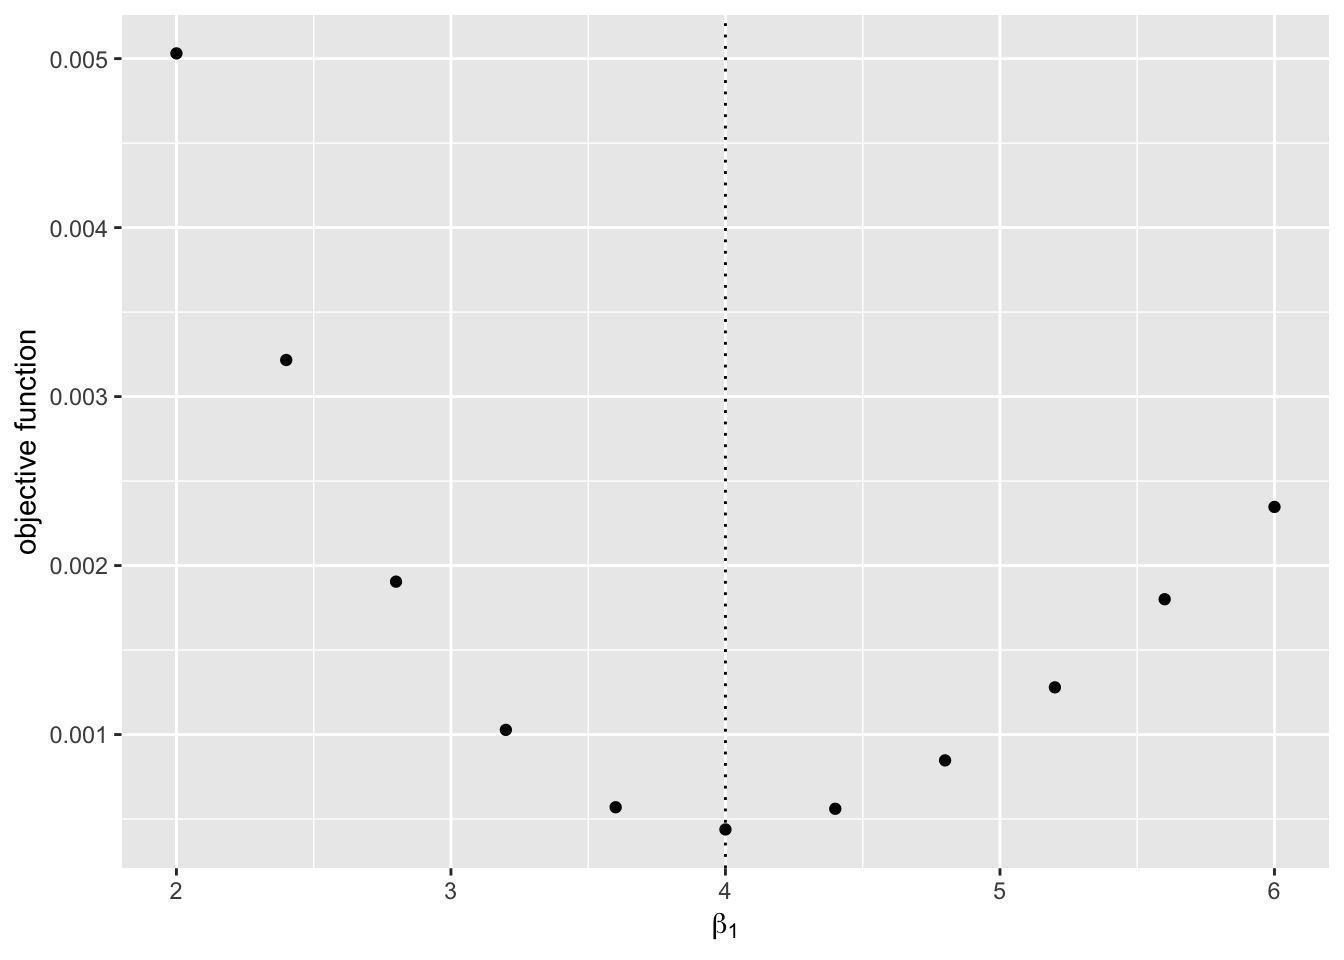
\includegraphics{lecture_files/figure-latex/unnamed-chunk-91-1} \end{center}

\begin{verbatim}
## 
## [[2]]
\end{verbatim}

\begin{center}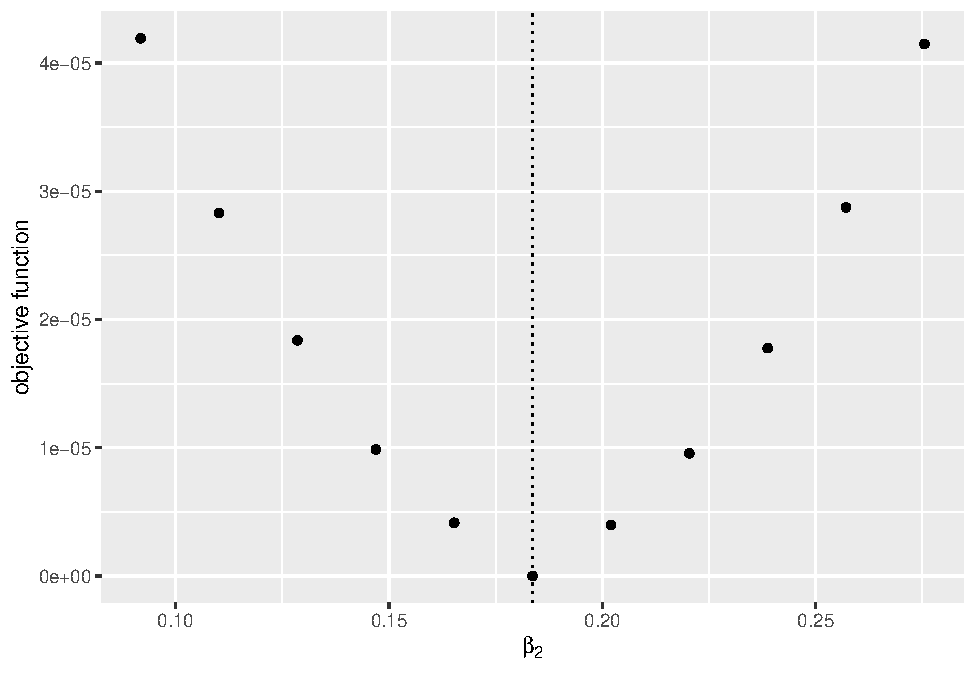
\includegraphics{lecture_files/figure-latex/unnamed-chunk-91-2} \end{center}

\begin{verbatim}
## 
## [[3]]
\end{verbatim}

\begin{center}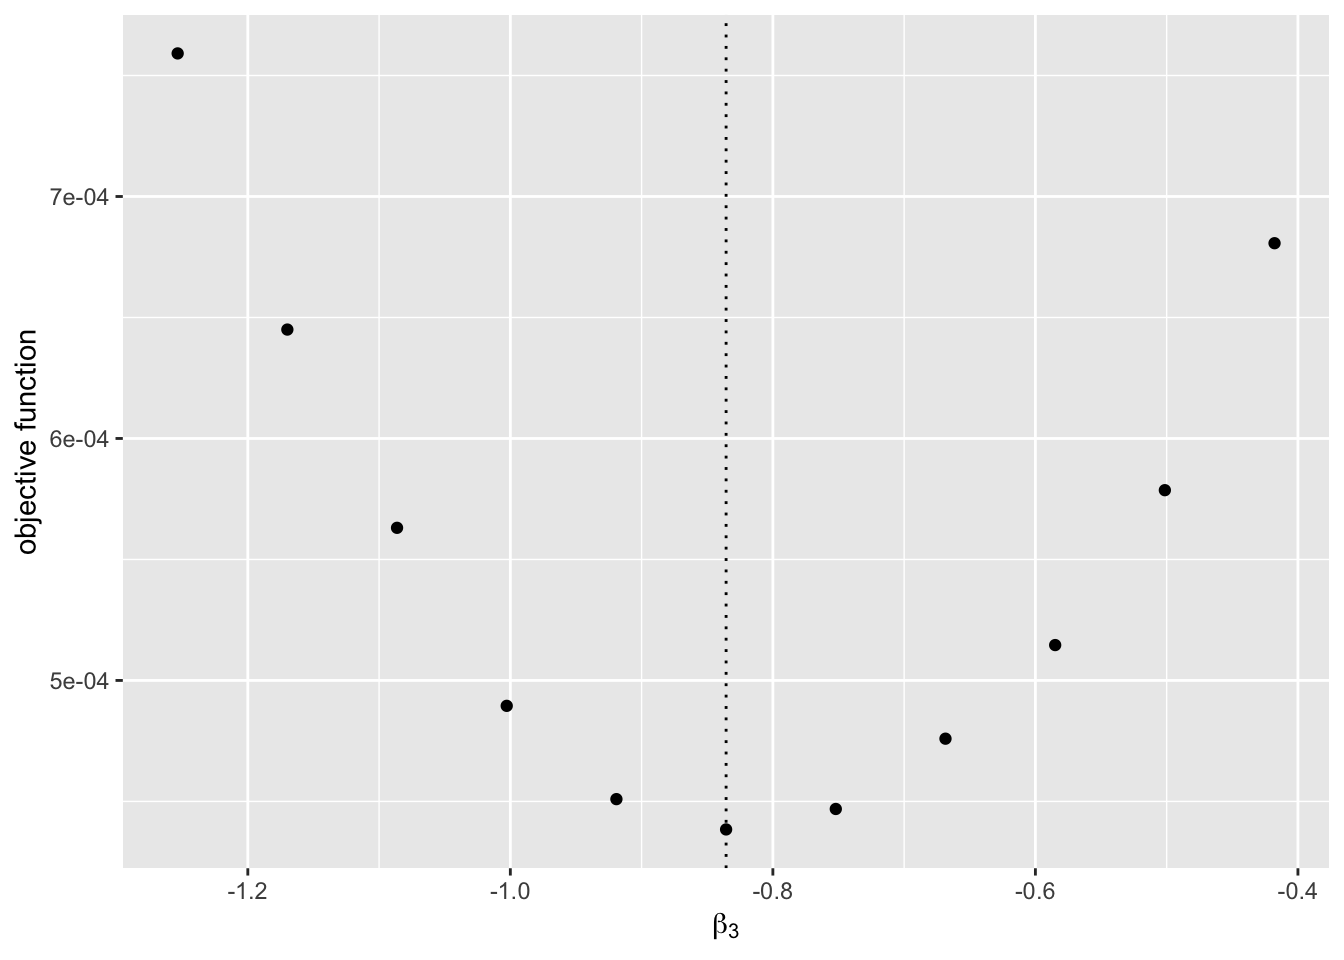
\includegraphics{lecture_files/figure-latex/unnamed-chunk-91-3} \end{center}

\begin{verbatim}
## 
## [[4]]
\end{verbatim}

\begin{center}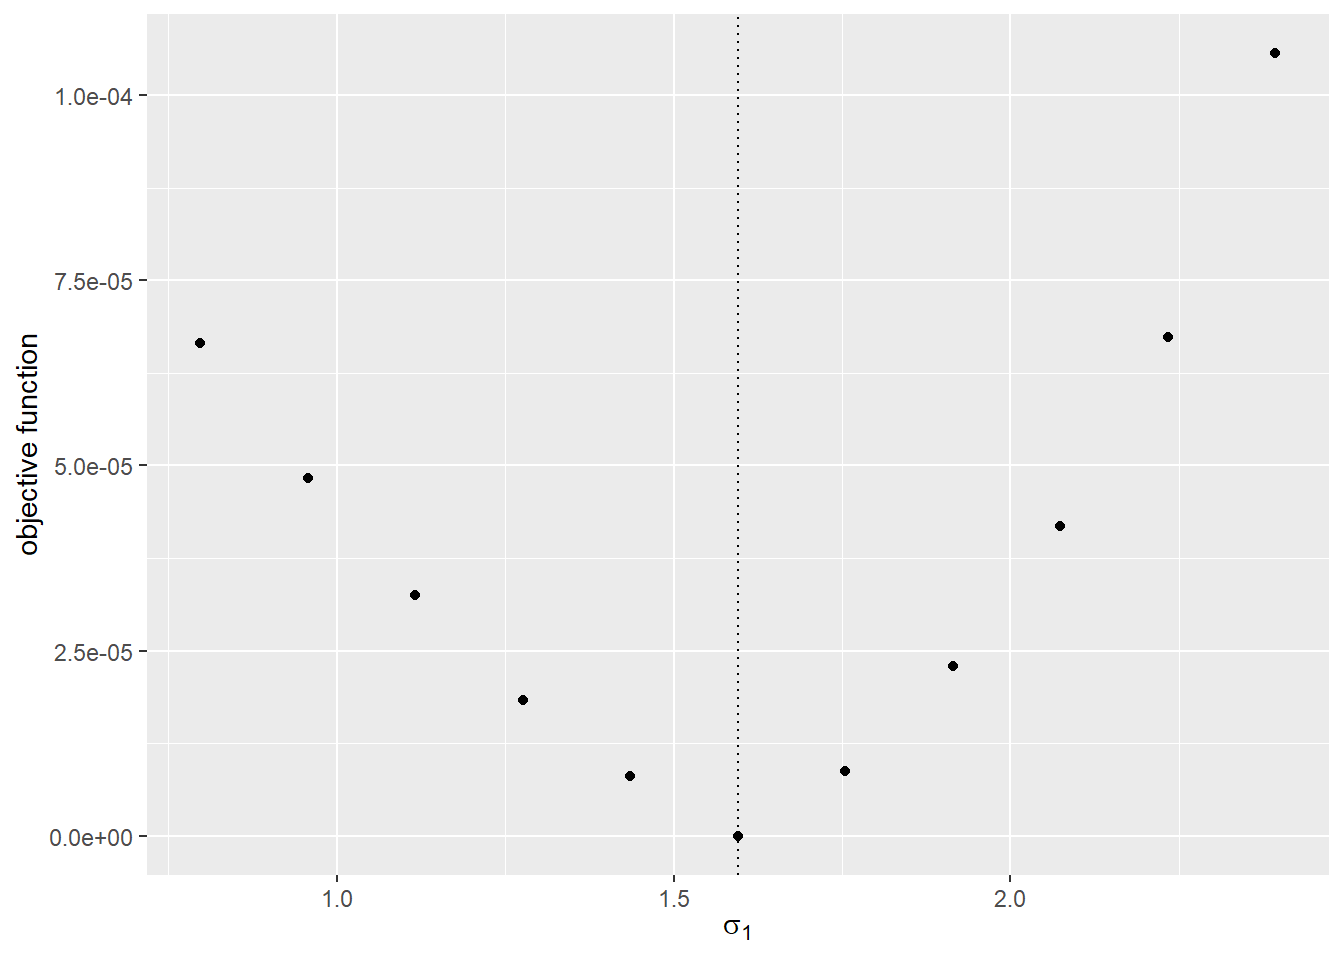
\includegraphics{lecture_files/figure-latex/unnamed-chunk-91-4} \end{center}

\begin{verbatim}
## 
## [[5]]
\end{verbatim}

\begin{center}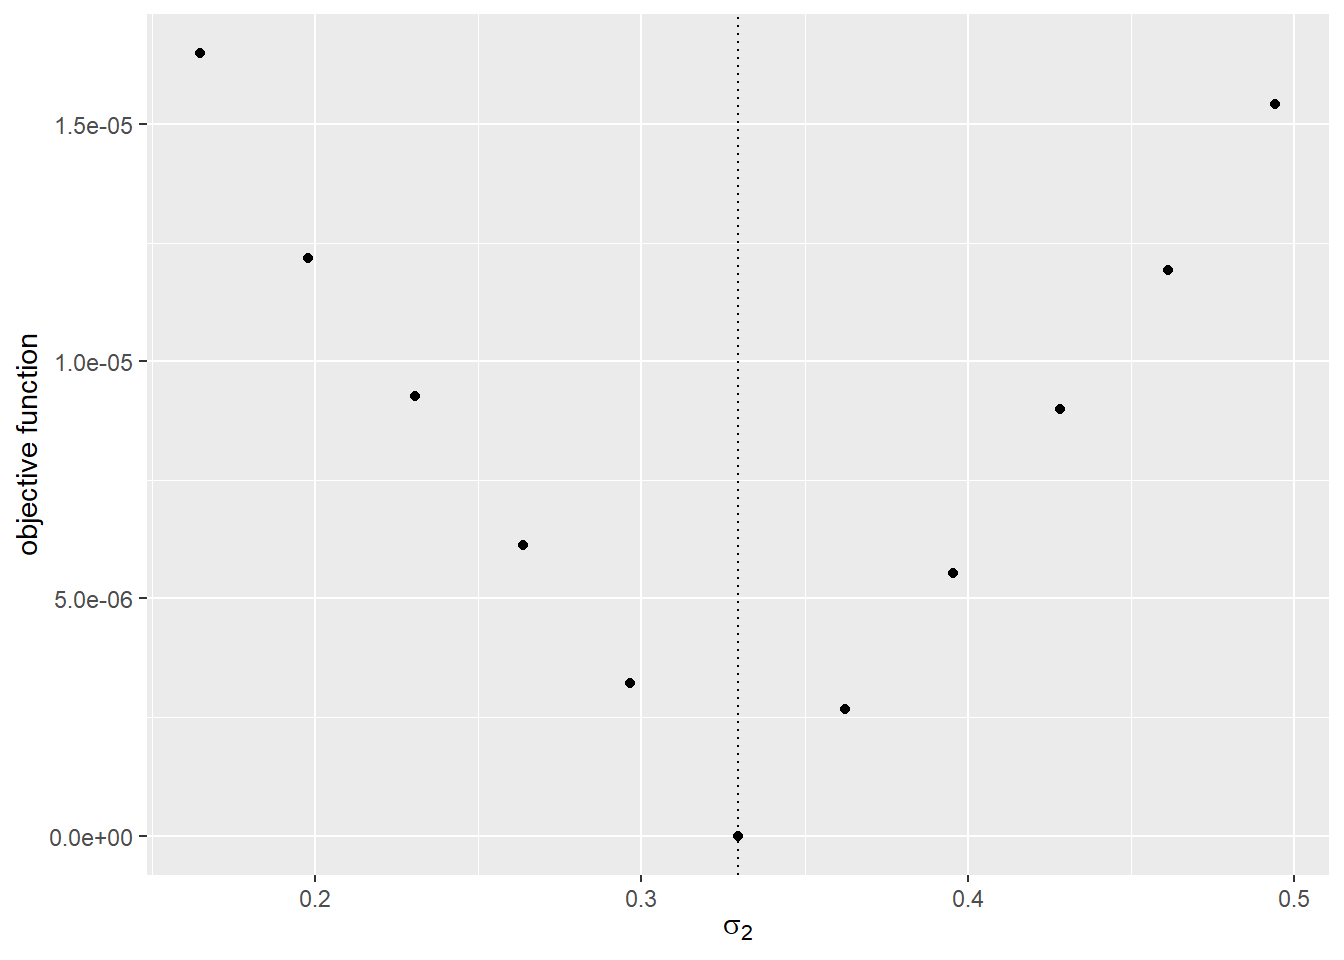
\includegraphics{lecture_files/figure-latex/unnamed-chunk-91-5} \end{center}

\begin{verbatim}
## 
## [[6]]
\end{verbatim}

\begin{center}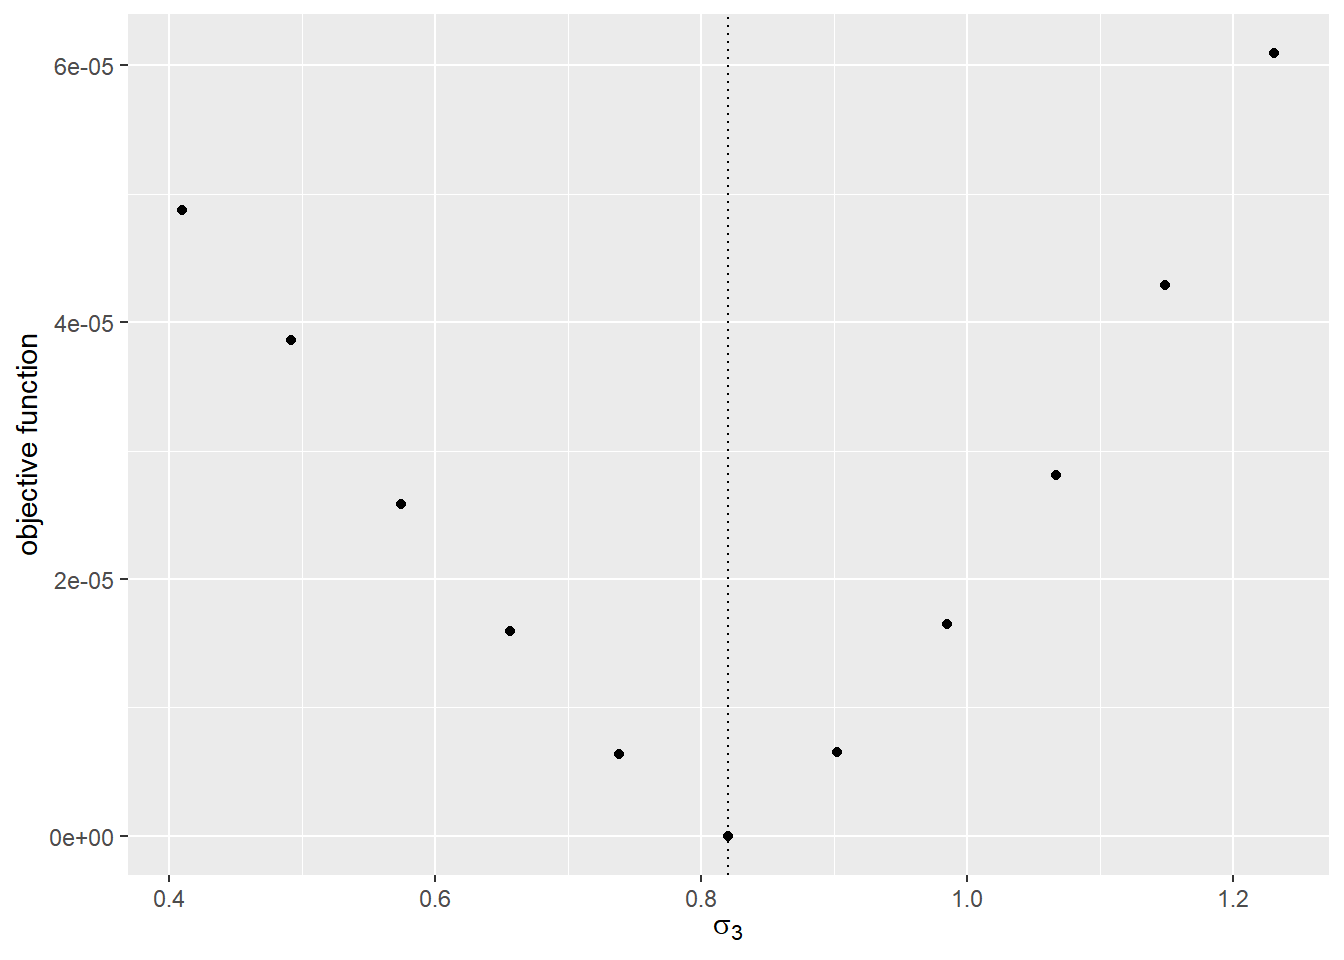
\includegraphics{lecture_files/figure-latex/unnamed-chunk-91-6} \end{center}

\begin{verbatim}
## 
## [[7]]
\end{verbatim}

\begin{center}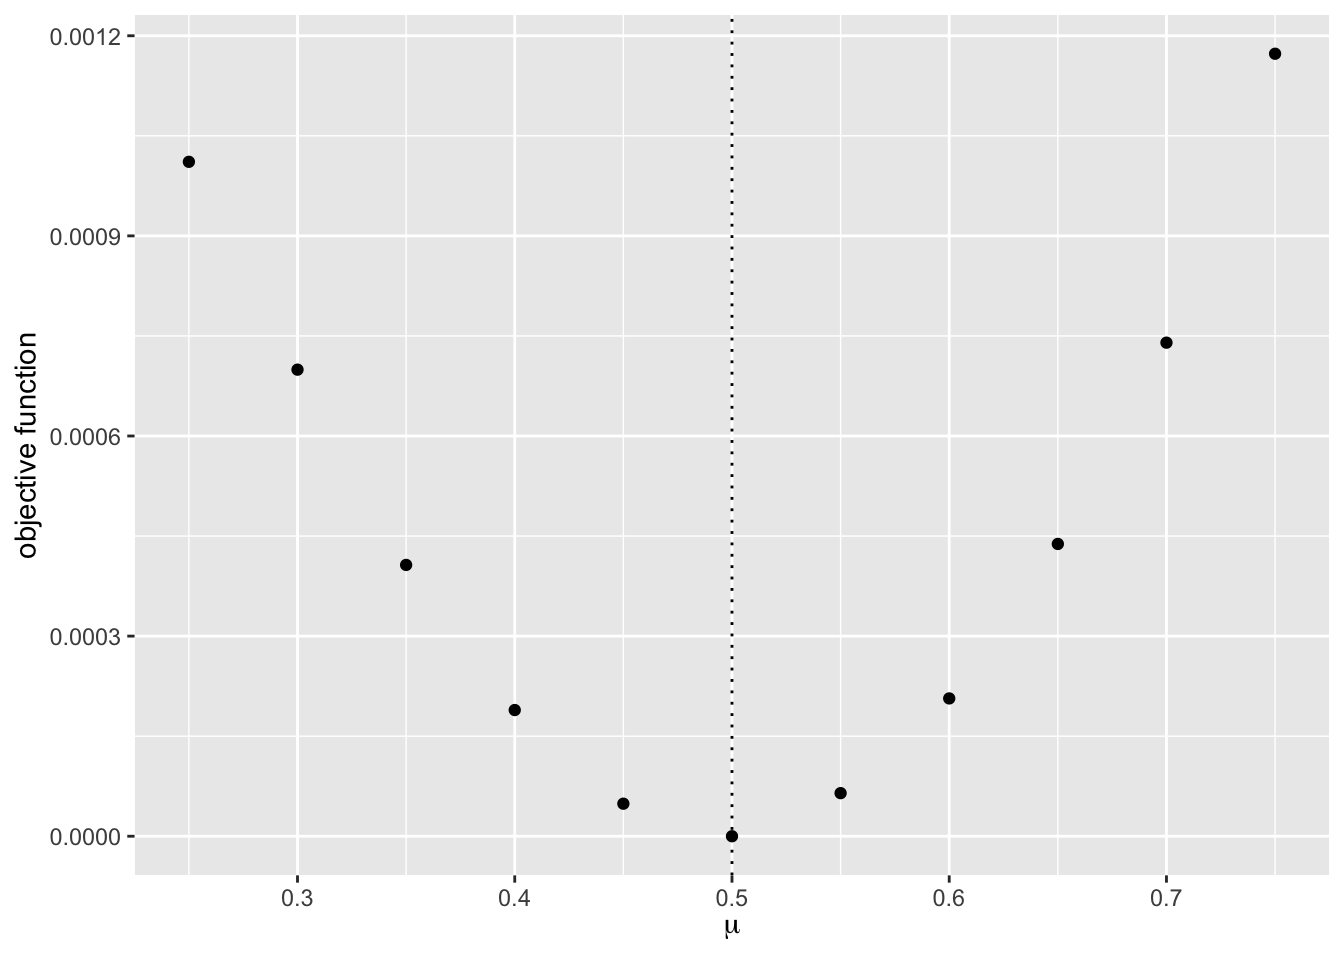
\includegraphics{lecture_files/figure-latex/unnamed-chunk-91-7} \end{center}

\begin{verbatim}
## 
## [[8]]
\end{verbatim}

\begin{center}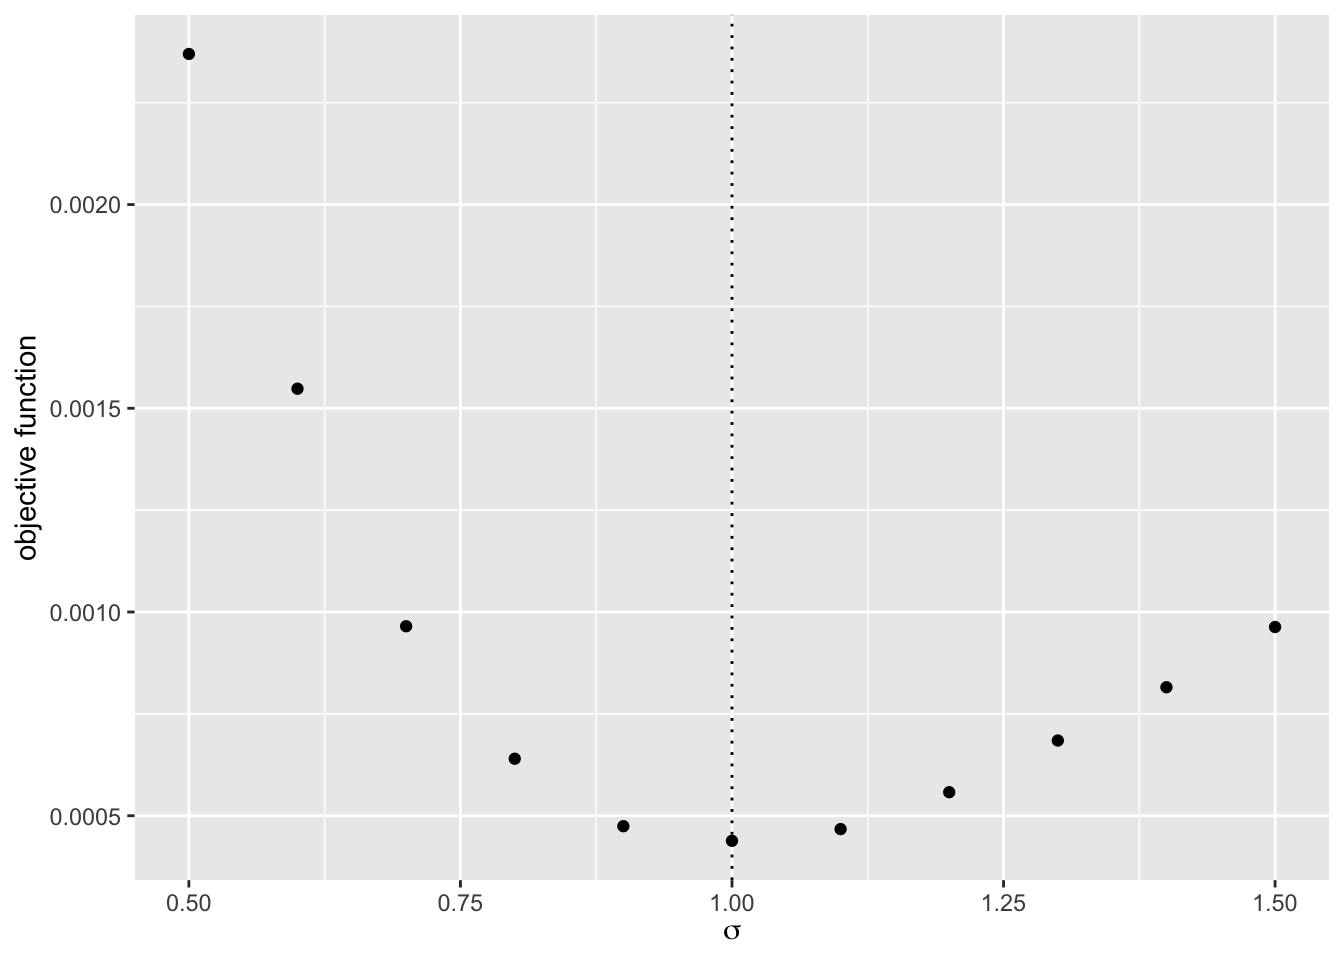
\includegraphics{lecture_files/figure-latex/unnamed-chunk-91-8} \end{center}

The graphs with the Monte Carlo shocks:

\begin{verbatim}
## [[1]]
\end{verbatim}

\begin{center}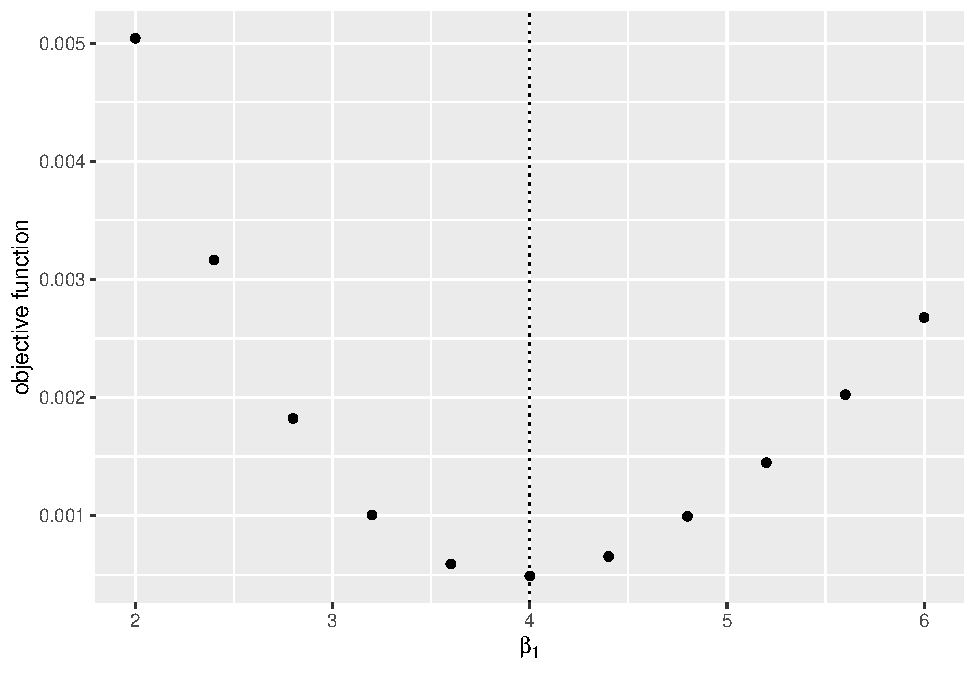
\includegraphics{lecture_files/figure-latex/unnamed-chunk-93-1} \end{center}

\begin{verbatim}
## 
## [[2]]
\end{verbatim}

\begin{center}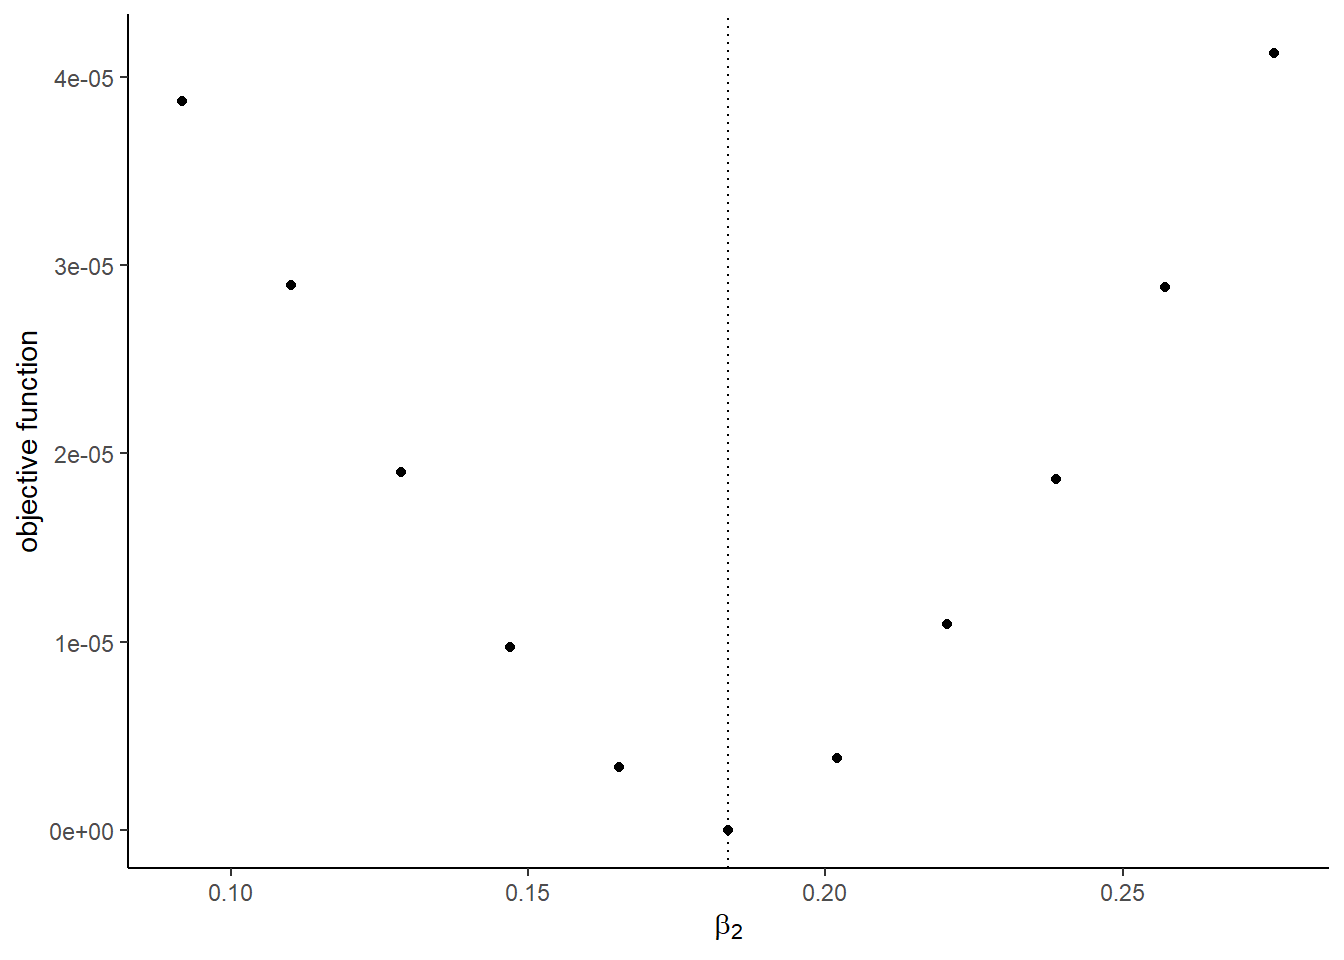
\includegraphics{lecture_files/figure-latex/unnamed-chunk-93-2} \end{center}

\begin{verbatim}
## 
## [[3]]
\end{verbatim}

\begin{center}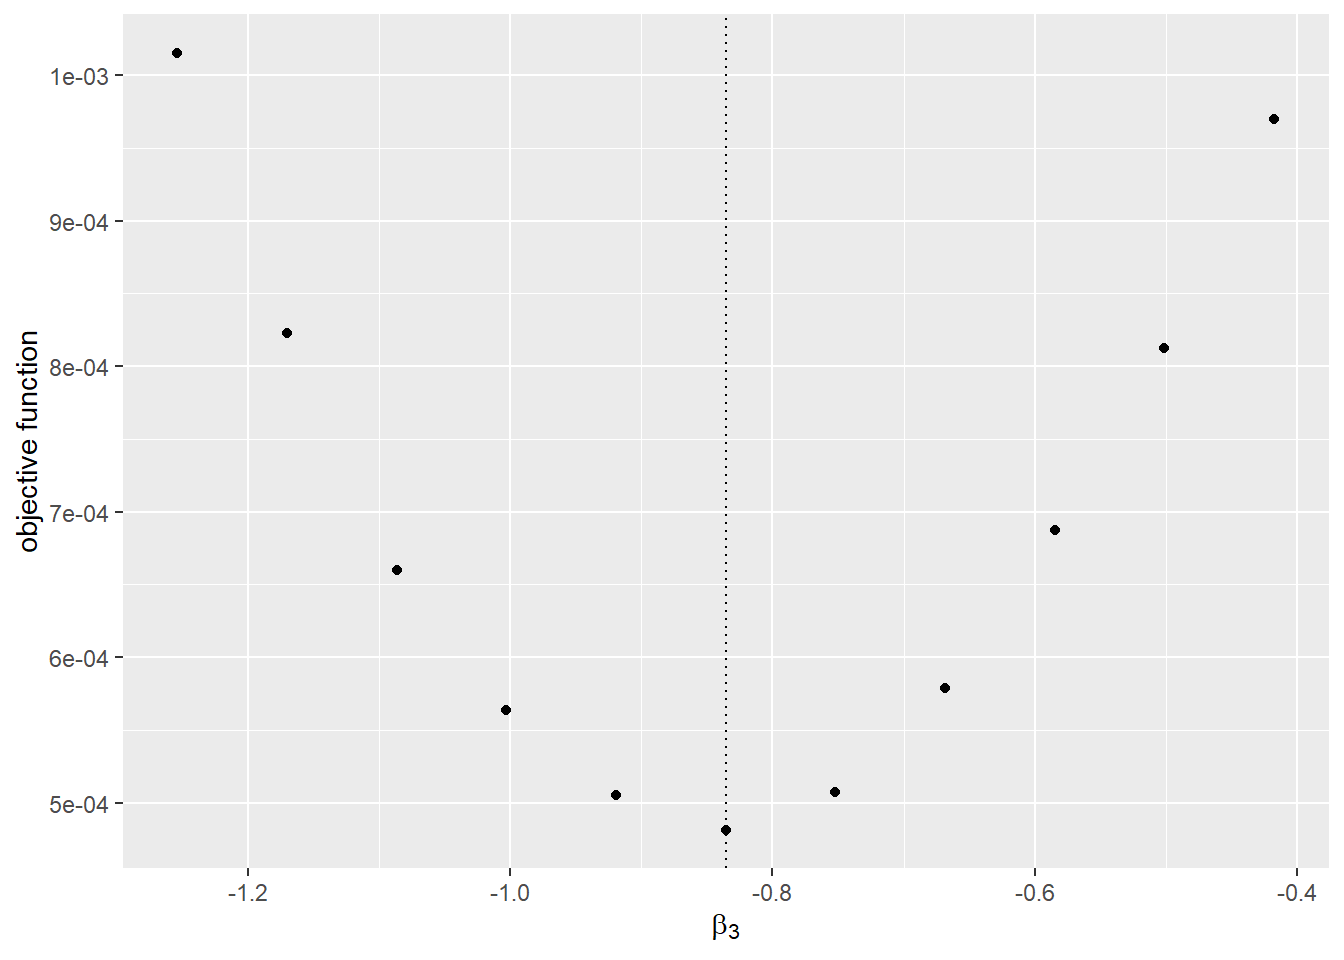
\includegraphics{lecture_files/figure-latex/unnamed-chunk-93-3} \end{center}

\begin{verbatim}
## 
## [[4]]
\end{verbatim}

\begin{center}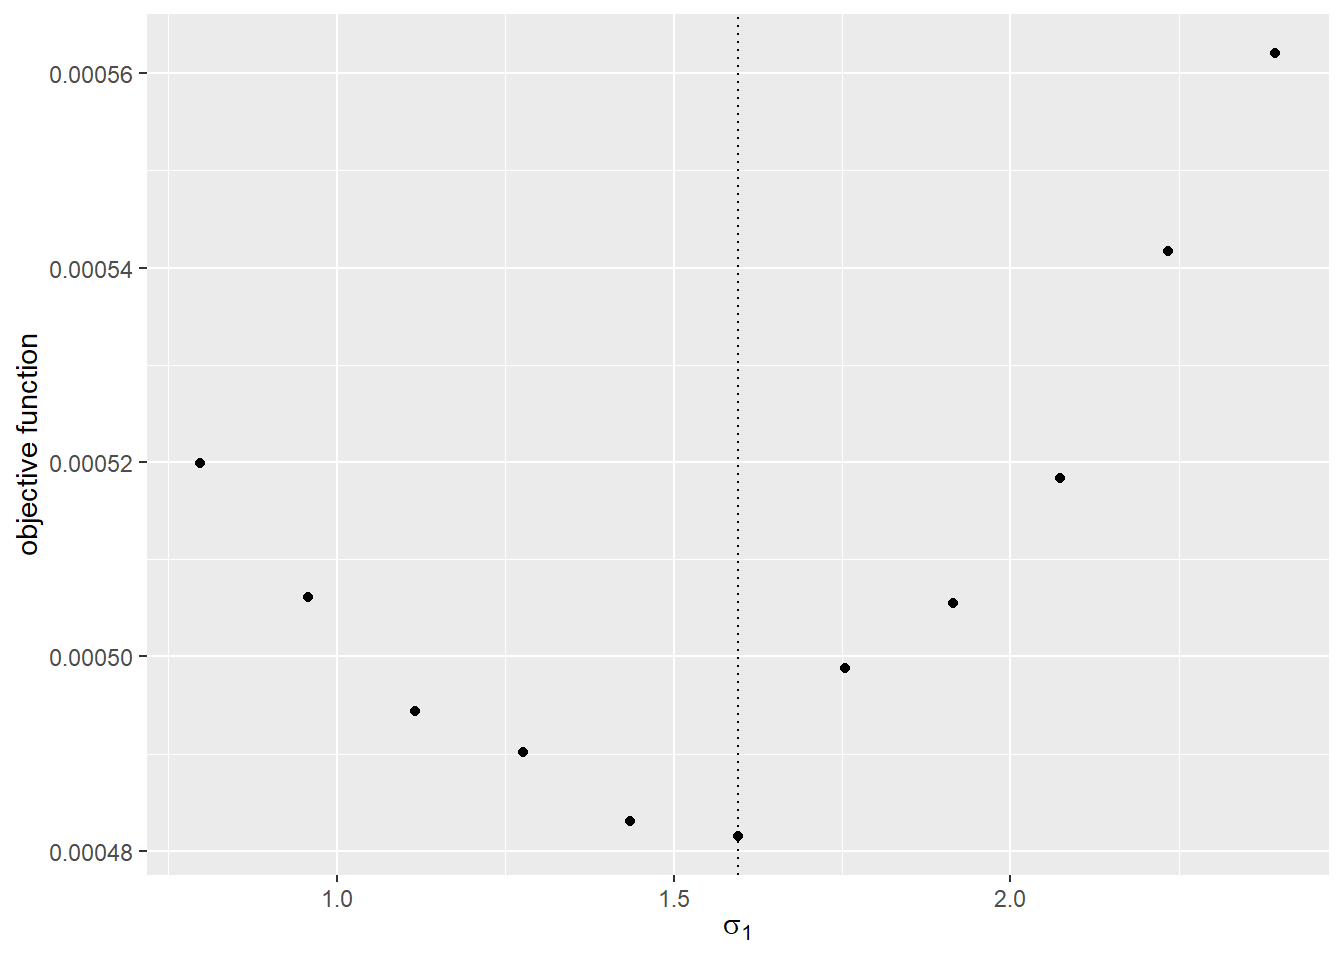
\includegraphics{lecture_files/figure-latex/unnamed-chunk-93-4} \end{center}

\begin{verbatim}
## 
## [[5]]
\end{verbatim}

\begin{center}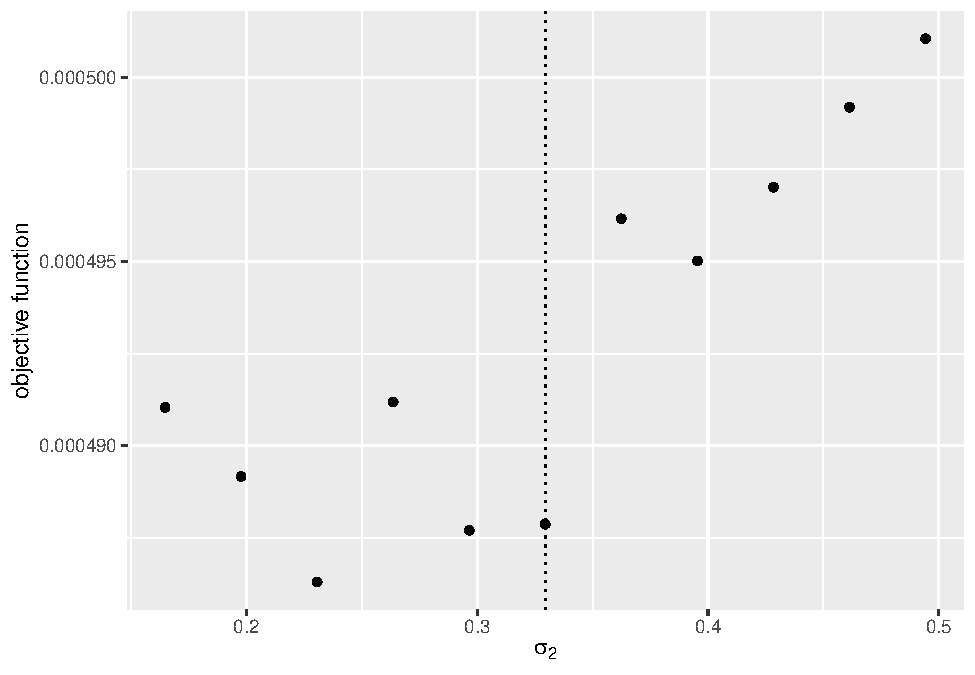
\includegraphics{lecture_files/figure-latex/unnamed-chunk-93-5} \end{center}

\begin{verbatim}
## 
## [[6]]
\end{verbatim}

\begin{center}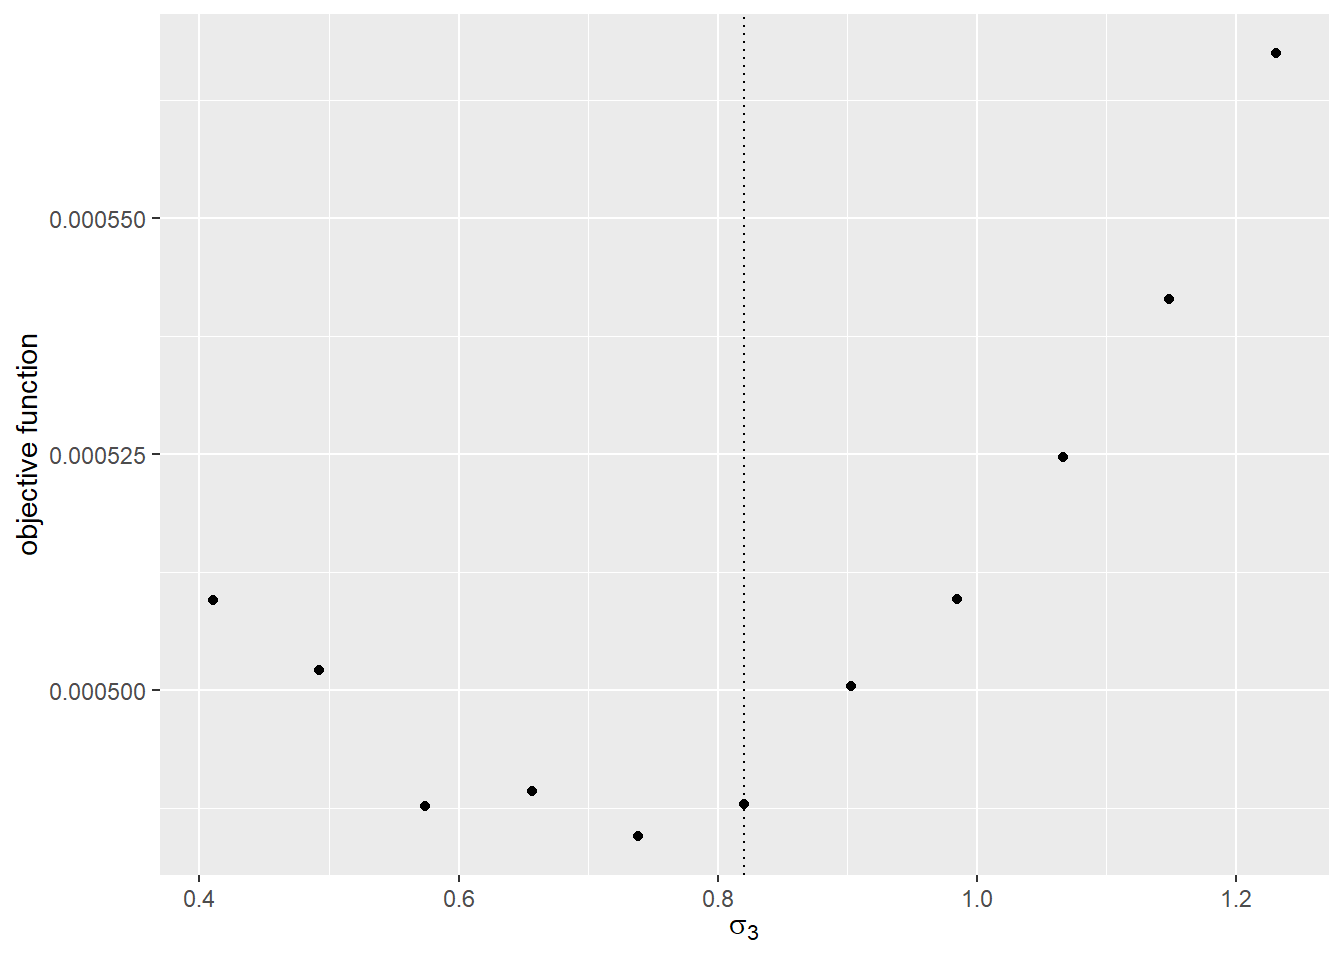
\includegraphics{lecture_files/figure-latex/unnamed-chunk-93-6} \end{center}

\begin{verbatim}
## 
## [[7]]
\end{verbatim}

\begin{center}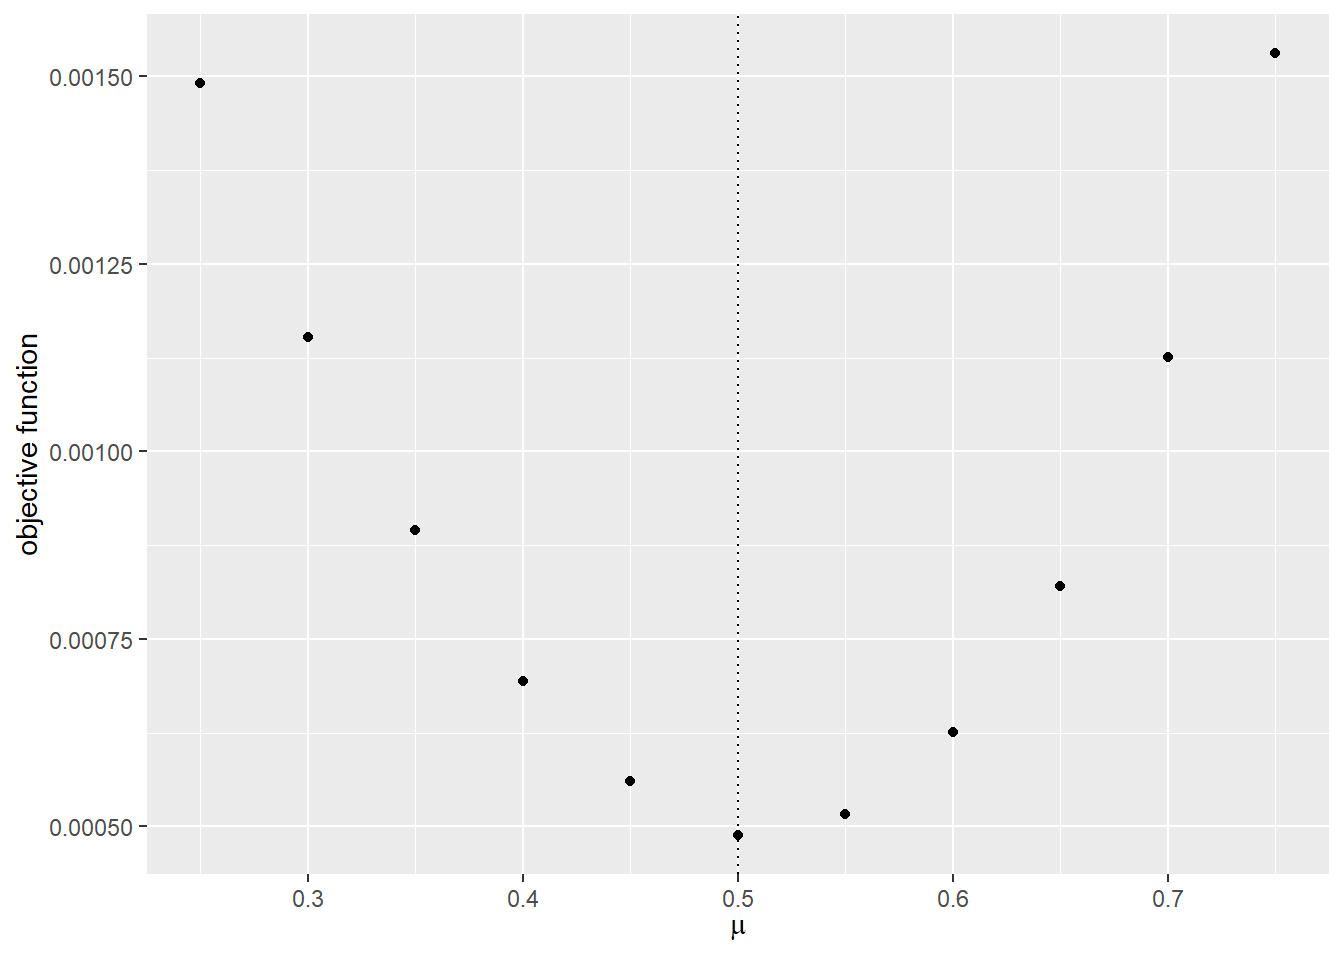
\includegraphics{lecture_files/figure-latex/unnamed-chunk-93-7} \end{center}

\begin{verbatim}
## 
## [[8]]
\end{verbatim}

\begin{center}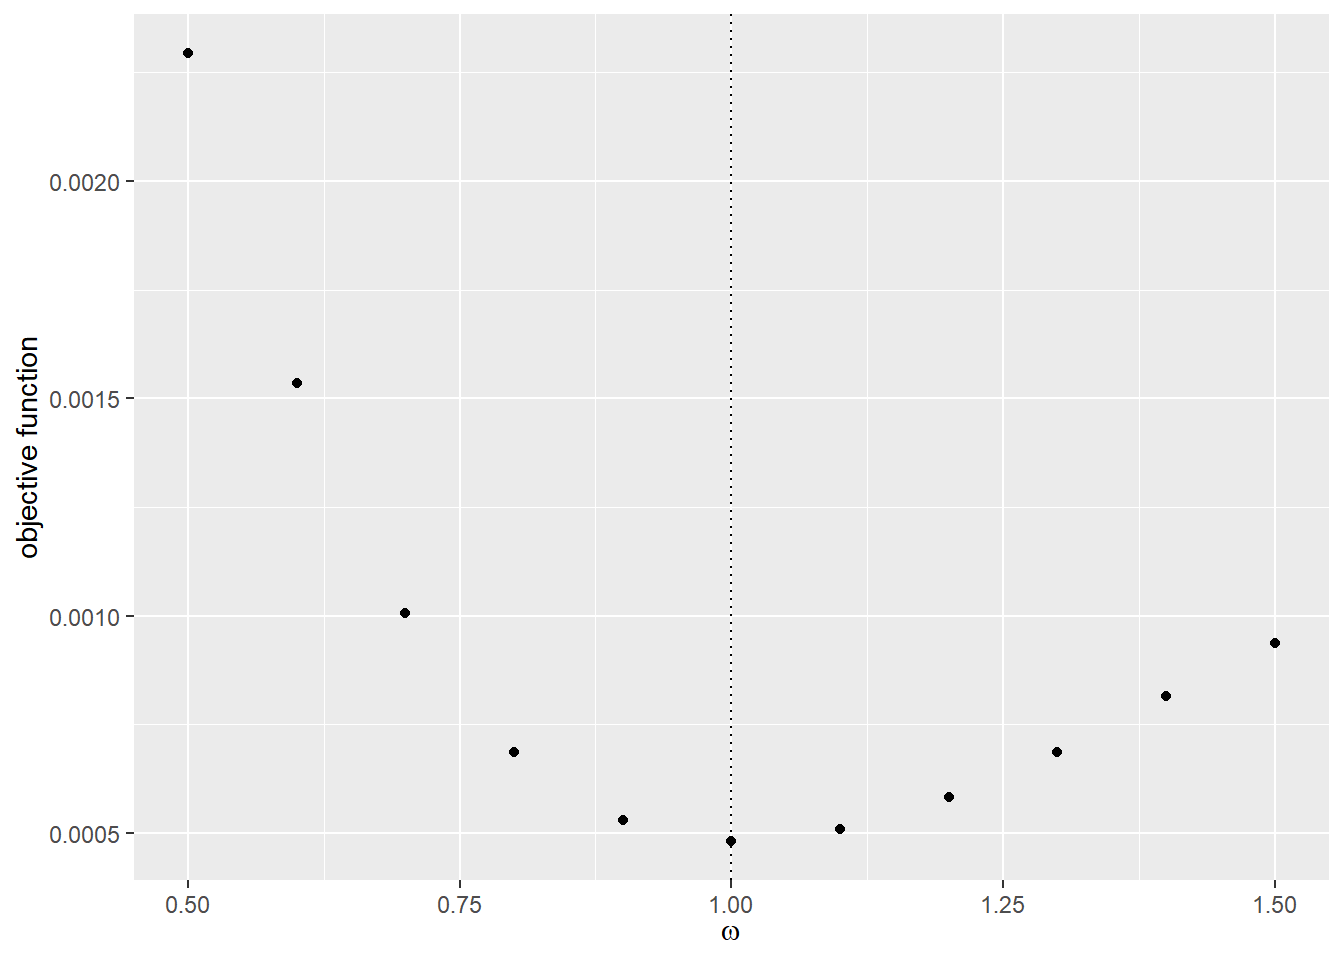
\includegraphics{lecture_files/figure-latex/unnamed-chunk-93-8} \end{center}

\begin{enumerate}
\def\labelenumi{\arabic{enumi}.}
\setcounter{enumi}{7}
\tightlist
\item
  Use \texttt{optim} to find the minimizer of the objective function
  using \texttt{Nelder-Mead} method. You can start from the true
  parameter values. Compare the estimates with the true parameters.
\end{enumerate}

\begin{verbatim}
## $par
## [1]  4.0425713  0.1841677 -0.8230489  1.6348574  0.3148886  0.7831262
## [7]  0.4998710  1.0138327
## 
## $value
## [1] 0.0004760686
## 
## $counts
## function gradient 
##      263       NA 
## 
## $convergence
## [1] 0
## 
## $message
## NULL
\end{verbatim}

\begin{verbatim}
##         true  estimates
## 1  4.0000000  4.0425713
## 2  0.1836433  0.1841677
## 3 -0.8356286 -0.8230489
## 4  1.5952808  1.6348574
## 5  0.3295078  0.3148886
## 6  0.8204684  0.7831262
## 7  0.5000000  0.4998710
## 8  1.0000000  1.0138327
\end{verbatim}

\chapter{Assignment 4: Demand Function Estimation II}\label{assignment4}

The deadline is \textbf{March 25 1:30pm}.

\section{Simulate data}\label{simulate-data-3}

\textbf{Be carefull that some parameters are changed from assignment 3}.
We simulate data from a discrete choice model that is the same with in
assignment 3 except for the existence of unobserved product-specific
fixed effects. There are \(T\) markets and each market has \(N\)
consumers. There are \(J\) products and the indirect utility of consumer
\(i\) in market \(t\) for product \(j\) is: \[
u_{itj} = \beta_{it}' x_j + \alpha_{it} p_{jt} + \xi_{jt} + \epsilon_{ijt},
\] where \(\epsilon_{ijt}\) is an i.i.d. type-I extreme random variable.
\(x_j\) is \(K\)-dimensional observed characteristics of the product.
\(p_{jt}\) is the retail price of the product in the market.

\(\xi_{jt}\) is product-market specific fixed effect. \(p_{jt}\) can be
correlated with \(\xi_{jt}\) but \(x_{jt}\)s are independent of
\(\xi_{jt}\). \(j = 0\) is an outside option whose indirect utility is:
\[
u_{it0} = \epsilon_{i0t},
\] where \(\epsilon_{i0t}\) is an i.i.d. type-I extreme random variable.

\(\beta_{it}\) and \(\alpha_{it}\) are different across consumers, and
they are distributed as: \[
\beta_{itk} = \beta_{0k} + \sigma_k \nu_{itk},
\] \[
\alpha_{it} = - \exp(\mu + \omega \upsilon_{it}) = - \exp(\mu + \frac{\omega^2}{2}) + [- \exp(\mu + \omega \upsilon_{it}) + \exp(\mu + \frac{\omega^2}{2})] \equiv \alpha_0 + \tilde{\alpha}_{it},
\] where \(\nu_{itk}\) for \(k = 1, \cdots, K\) and \(\upsilon_{it}\)
are i.i.d. standard normal random variables. \(\alpha_0\) is the mean of
\(\alpha_i\) and \(\tilde{\alpha}_i\) is the deviation from the mean.

Given a choice set in the market, \(\mathcal{J}_t \cup \{0\}\), a
consumer chooses the alternative that maximizes her utility: \[
q_{ijt} = 1\{u_{ijt} = \max_{k \in \mathcal{J}_t \cup \{0\}} u_{ikt}\}.
\] The choice probability of product \(j\) for consumer \(i\) in market
\(t\) is: \[
\sigma_{jt}(p_t, x_t, \xi_t) = \mathbb{P}\{u_{ijt} = \max_{k \in \mathcal{J}_t \cup \{0\}} u_{ikt}\}.
\]

Suppose that we only observe the share data: \[
s_{jt} = \frac{1}{N} \sum_{i = 1}^N q_{ijt},
\] along with the product-market characteristics \(x_{jt}\) and the
retail prices \(p_{jt}\) for \(j \in \mathcal{J}_t \cup \{0\}\) for
\(t = 1, \cdots, T\). We do not observe the choice data \(q_{ijt}\) nor
shocks \(\xi_{jt}, \nu_{it}, \upsilon_{it}, \epsilon_{ijt}\).

We draw \(\xi_{jt}\) from i.i.d. normal distribution with mean 0 and
standard deviation \(\sigma_{\xi}\).

\begin{enumerate}
\def\labelenumi{\arabic{enumi}.}
\tightlist
\item
  Set the seed, constants, and parameters of interest as follows.
\end{enumerate}

\begin{Shaded}
\begin{Highlighting}[]
\CommentTok{# set the seed}
\KeywordTok{set.seed}\NormalTok{(}\DecValTok{1}\NormalTok{)}
\CommentTok{# number of products}
\NormalTok{J <-}\StringTok{ }\DecValTok{10}
\CommentTok{# dimension of product characteristics including the intercept}
\NormalTok{K <-}\StringTok{ }\DecValTok{3}
\CommentTok{# number of markets}
\NormalTok{T <-}\StringTok{ }\DecValTok{100}
\CommentTok{# number of consumers per market}
\NormalTok{N <-}\StringTok{ }\DecValTok{500}
\CommentTok{# number of Monte Carlo}
\NormalTok{L <-}\StringTok{ }\DecValTok{500}
\end{Highlighting}
\end{Shaded}

\begin{Shaded}
\begin{Highlighting}[]
\CommentTok{# set parameters of interests}
\NormalTok{beta <-}\StringTok{ }\KeywordTok{rnorm}\NormalTok{(K); }
\NormalTok{beta[}\DecValTok{1}\NormalTok{] <-}\StringTok{ }\DecValTok{4}
\NormalTok{beta}
\end{Highlighting}
\end{Shaded}

\begin{verbatim}
## [1]  4.0000000  0.1836433 -0.8356286
\end{verbatim}

\begin{Shaded}
\begin{Highlighting}[]
\NormalTok{sigma <-}\StringTok{ }\KeywordTok{abs}\NormalTok{(}\KeywordTok{rnorm}\NormalTok{(K)); sigma}
\end{Highlighting}
\end{Shaded}

\begin{verbatim}
## [1] 1.5952808 0.3295078 0.8204684
\end{verbatim}

\begin{Shaded}
\begin{Highlighting}[]
\NormalTok{mu <-}\StringTok{ }\FloatTok{0.5}
\NormalTok{omega <-}\StringTok{ }\DecValTok{1}
\end{Highlighting}
\end{Shaded}

Generate the covariates as follows.

The product-market characteristics: \[
x_{j1} = 1, x_{jk} \sim N(0, \sigma_x), k = 2, \cdots, K,
\] where \(\sigma_x\) is referred to as \texttt{sd\_x} in the code.

The product-market-specific unobserved fixed effect: \[
\xi_{jt} \sim N(0, \sigma_\xi),
\] where \(\sigma_xi\) is referred to as \texttt{sd\_xi} in the code.

The marginal cost of product \(j\) in market \(t\): \[
c_{jt} \sim \text{logNormal}(0, \sigma_c),
\] where \(\sigma_c\) is referred to as \texttt{sd\_c} in the code.

The retail price: \[
p_{jt} - c_{jt} \sim \text{logNorm}(\gamma \xi_{jt}, \sigma_p),
\] where \(\gamma\) is referred to as \texttt{price\_xi} and
\(\sigma_p\) as \texttt{sd\_p} in the code. This price is not the
equilibrium price. We will revisit this point in a subsequent
assignment.

The value of the auxiliary parameters are set as follows:

\begin{Shaded}
\begin{Highlighting}[]
\CommentTok{# set auxiliary parameters}
\NormalTok{price_xi <-}\StringTok{ }\DecValTok{1}
\NormalTok{sd_x <-}\StringTok{ }\DecValTok{2}
\NormalTok{sd_xi <-}\StringTok{ }\FloatTok{0.5}
\NormalTok{sd_c <-}\StringTok{ }\FloatTok{0.05}
\NormalTok{sd_p <-}\StringTok{ }\FloatTok{0.05}
\end{Highlighting}
\end{Shaded}

\begin{enumerate}
\def\labelenumi{\arabic{enumi}.}
\setcounter{enumi}{1}
\tightlist
\item
  \texttt{X} is the data frame such that a row contains the
  characteristics vector \(x_{j}\) of a product and columns are product
  index and observed product characteristics. The dimension of the
  characteristics \(K\) is specified above. Add the row of the outside
  option whose index is \(0\) and all the characteristics are zero.
\end{enumerate}

\begin{Shaded}
\begin{Highlighting}[]
\NormalTok{X}
\end{Highlighting}
\end{Shaded}

\begin{verbatim}
## # A tibble: 11 x 4
##        j   x_1     x_2     x_3
##    <dbl> <dbl>   <dbl>   <dbl>
##  1     0     0  0       0     
##  2     1     1  0.975  -0.0324
##  3     2     1  1.48    1.89  
##  4     3     1  1.15    1.64  
##  5     4     1 -0.611   1.19  
##  6     5     1  3.02    1.84  
##  7     6     1  0.780   1.56  
##  8     7     1 -1.24    0.149 
##  9     8     1 -4.43   -3.98  
## 10     9     1  2.25    1.24  
## 11    10     1 -0.0899 -0.112
\end{verbatim}

\begin{enumerate}
\def\labelenumi{\arabic{enumi}.}
\setcounter{enumi}{2}
\tightlist
\item
  \texttt{M} is the data frame such that a row contains the price
  \(\xi_{jt}\), marginal cost \(c_{jt}\), and price \(p_{jt}\). After
  generating the variables, drop some products in each market.
  \textbf{In this assignment, we drop products in a different way from
  the last assignment}. In order to change the number of available
  products in each market, for each market, first draw \(J_t\) from a
  discrete uniform distribution between \(1\) and \(J\). Then, drop
  products from each market using \texttt{dplyr::sample\_frac} function
  with the realized number of available products. The variation in the
  available products is important for the identification of the
  distribution of consumer-level unobserved heterogeneity. Add the row
  of the outside option to each market whose index is \(0\) and all the
  variables take value zero.
\end{enumerate}

\begin{Shaded}
\begin{Highlighting}[]
\NormalTok{M}
\end{Highlighting}
\end{Shaded}

\begin{verbatim}
## # A tibble: 746 x 5
##        j     t      xi     c     p
##    <dbl> <int>   <dbl> <dbl> <dbl>
##  1     0     1  0      0      0   
##  2     6     1 -0.0514 0.980  1.91
##  3     0     2  0      0      0   
##  4     1     2 -0.197  0.988  1.90
##  5    10     2 -0.354  1.05   1.82
##  6     0     3  0      0      0   
##  7     1     3  0.182  1.04   2.22
##  8     2     3  0.384  1.01   2.61
##  9     3     3 -0.0562 1.02   2.01
## 10     4     3  0.441  1.01   2.62
## # ... with 736 more rows
\end{verbatim}

\begin{enumerate}
\def\labelenumi{\arabic{enumi}.}
\setcounter{enumi}{3}
\tightlist
\item
  Generate the consumer-level heterogeneity. \texttt{V} is the data
  frame such that a row contains the vector of shocks to consumer-level
  heterogeneity, \((\nu_{i}', \upsilon_i)\). They are all i.i.d.
  standard normal random variables.
\end{enumerate}

\begin{Shaded}
\begin{Highlighting}[]
\NormalTok{V}
\end{Highlighting}
\end{Shaded}

\begin{verbatim}
## # A tibble: 50,000 x 6
##        i     t   v_x_1  v_x_2   v_x_3    v_p
##    <int> <int>   <dbl>  <dbl>   <dbl>  <dbl>
##  1     1     1  1.16   -1.40   0.0786 -1.15 
##  2     2     1 -1.05   -0.149  1.08    0.623
##  3     3     1 -0.426  -4.21   0.625  -1.14 
##  4     4     1 -0.235   0.463  0.470   0.241
##  5     5     1  1.19   -0.342  0.169   0.160
##  6     6     1  0.541   0.525  0.305   1.72 
##  7     7     1 -0.0893 -0.434  2.18   -0.432
##  8     8     1 -0.712   0.747 -0.306  -0.527
##  9     9     1  0.504   1.11   1.70   -1.75 
## 10    10     1 -0.107   1.83  -0.841   0.693
## # ... with 49,990 more rows
\end{verbatim}

\begin{enumerate}
\def\labelenumi{\arabic{enumi}.}
\setcounter{enumi}{4}
\tightlist
\item
  Join \texttt{X}, \texttt{M}, \texttt{V} using
  \texttt{dplyr::left\_join} and name it \texttt{df}. \texttt{df} is the
  data frame such that a row contains variables for a consumer about a
  product that is available in a market.
\end{enumerate}

\begin{Shaded}
\begin{Highlighting}[]
\NormalTok{df}
\end{Highlighting}
\end{Shaded}

\begin{verbatim}
## # A tibble: 373,000 x 13
##        t     i     j  v_x_1  v_x_2  v_x_3    v_p   x_1   x_2   x_3      xi
##    <int> <int> <dbl>  <dbl>  <dbl>  <dbl>  <dbl> <dbl> <dbl> <dbl>   <dbl>
##  1     1     1     0  1.16  -1.40  0.0786 -1.15      0 0      0     0     
##  2     1     1     6  1.16  -1.40  0.0786 -1.15      1 0.780  1.56 -0.0514
##  3     1     2     0 -1.05  -0.149 1.08    0.623     0 0      0     0     
##  4     1     2     6 -1.05  -0.149 1.08    0.623     1 0.780  1.56 -0.0514
##  5     1     3     0 -0.426 -4.21  0.625  -1.14      0 0      0     0     
##  6     1     3     6 -0.426 -4.21  0.625  -1.14      1 0.780  1.56 -0.0514
##  7     1     4     0 -0.235  0.463 0.470   0.241     0 0      0     0     
##  8     1     4     6 -0.235  0.463 0.470   0.241     1 0.780  1.56 -0.0514
##  9     1     5     0  1.19  -0.342 0.169   0.160     0 0      0     0     
## 10     1     5     6  1.19  -0.342 0.169   0.160     1 0.780  1.56 -0.0514
## # ... with 372,990 more rows, and 2 more variables: c <dbl>, p <dbl>
\end{verbatim}

\begin{enumerate}
\def\labelenumi{\arabic{enumi}.}
\setcounter{enumi}{5}
\tightlist
\item
  Draw a vector of preference shocks \texttt{e} whose length is the same
  as the number of rows of \texttt{df}.
\end{enumerate}

\begin{Shaded}
\begin{Highlighting}[]
\KeywordTok{head}\NormalTok{(e)}
\end{Highlighting}
\end{Shaded}

\begin{verbatim}
## [1]  0.2262454  1.3417639 -0.1693913  0.8906905  0.5558130  1.9909058
\end{verbatim}

\begin{enumerate}
\def\labelenumi{\arabic{enumi}.}
\setcounter{enumi}{6}
\tightlist
\item
  Write a function
  \texttt{compute\_indirect\_utility(df,\ beta,\ sigma,\ mu,\ omega)}
  that returns a vector whose element is the mean indirect utility of a
  product for a consumer in a market. The output should have the same
  length with \(e\). (This function is the same with assignment 3. You
  can use the function.)
\end{enumerate}

\begin{Shaded}
\begin{Highlighting}[]
\CommentTok{# compute indirect utility}
\NormalTok{u <-}\StringTok{ }
\StringTok{  }\KeywordTok{compute_indirect_utility}\NormalTok{(}
\NormalTok{    df, beta, sigma, }
\NormalTok{           mu, omega)}
\KeywordTok{head}\NormalTok{(u)}
\end{Highlighting}
\end{Shaded}

\begin{verbatim}
##               u
## [1,]  0.0000000
## [2,]  3.3750542
## [3,]  0.0000000
## [4,] -3.3983588
## [5,]  0.0000000
## [6,]  0.8235142
\end{verbatim}

In the previous assingment, we computed predicted share by simulating
choice and taking their average. Instead, we compute the actual share
by: \[
s_{jt} = \frac{1}{N} \sum_{i = 1}^N \frac{\exp[\beta_{it}' x_j + \alpha_{it} p_{jt} + \xi_{jt}]}{1 + \sum_{k \in \mathcal{J}_t} \exp[\beta_{it}' x_k + \alpha_{it} p_{kt} + \xi_{jt}]}
\] and the predicted share by: \[
\widehat{\sigma}_{j}(x, p_t, \xi_t) = \frac{1}{L} \sum_{l = 1}^L \frac{\exp[\beta_{t}^{(l)\prime} x_j + \alpha_{t}^{(l)} p_{jt} + \xi_{jt}]}{1 + \sum_{k \in \mathcal{J}_t} \exp[\beta_{t}^{(l)\prime} x_k + \alpha_{t}^{(l)} p_{kt} + \xi_{jt}]}.
\]

\begin{enumerate}
\def\labelenumi{\arabic{enumi}.}
\setcounter{enumi}{7}
\tightlist
\item
  To do so, write a function
  \texttt{compute\_choice\_smooth(X,\ M,\ V,\ beta,\ sigma,\ mu,\ omega)}
  in which the choice of each consumer is not: \[
  q_{ijt} = 1\{u_{ijt} = \max_{k \in \mathcal{J}_t \cup \{0\}} u_{ikt}\},
  \] but \[
  \tilde{q}_{ijt} = \frac{\exp(u_{ijt})}{1 + \sum_{k \in \mathcal{J}_t} \exp(u_{ikt})}.
  \]
\end{enumerate}

\begin{Shaded}
\begin{Highlighting}[]
\NormalTok{df_choice_smooth <-}
\StringTok{  }\KeywordTok{compute_choice_smooth}\NormalTok{(X, M, V, beta, sigma, mu, omega)}
\KeywordTok{summary}\NormalTok{(df_choice_smooth)}
\end{Highlighting}
\end{Shaded}

\begin{verbatim}
##        t                i               j              v_x_1          
##  Min.   :  1.00   Min.   :  1.0   Min.   : 0.000   Min.   :-4.302781  
##  1st Qu.: 26.00   1st Qu.:125.8   1st Qu.: 2.000   1st Qu.:-0.685447  
##  Median : 51.50   Median :250.5   Median : 5.000   Median :-0.000461  
##  Mean   : 51.26   Mean   :250.5   Mean   : 4.807   Mean   :-0.005284  
##  3rd Qu.: 77.00   3rd Qu.:375.2   3rd Qu.: 8.000   3rd Qu.: 0.665219  
##  Max.   :100.00   Max.   :500.0   Max.   :10.000   Max.   : 3.809895  
##      v_x_2               v_x_3                v_p           
##  Min.   :-4.542122   Min.   :-3.957618   Min.   :-4.218131  
##  1st Qu.:-0.678377   1st Qu.:-0.676638   1st Qu.:-0.672011  
##  Median : 0.001435   Median : 0.006281   Median : 0.002166  
##  Mean   :-0.001076   Mean   : 0.003433   Mean   :-0.001402  
##  3rd Qu.: 0.671827   3rd Qu.: 0.679273   3rd Qu.: 0.674681  
##  Max.   : 4.313621   Max.   : 4.244194   Max.   : 4.074300  
##       x_1             x_2               x_3                 xi           
##  Min.   :0.000   Min.   :-4.4294   Min.   :-3.97870   Min.   :-1.444460  
##  1st Qu.:1.000   1st Qu.:-0.6108   1st Qu.:-0.03238   1st Qu.:-0.286633  
##  Median :1.000   Median : 0.7797   Median : 1.18780   Median : 0.000000  
##  Mean   :0.866   Mean   : 0.2713   Mean   : 0.44050   Mean   : 0.009578  
##  3rd Qu.:1.000   3rd Qu.: 1.4766   3rd Qu.: 1.64244   3rd Qu.: 0.317352  
##  Max.   :1.000   Max.   : 3.0236   Max.   : 1.88767   Max.   : 1.905138  
##        c                p               u                  q            
##  Min.   :0.0000   Min.   :0.000   Min.   :-284.515   Min.   :0.0000000  
##  1st Qu.:0.9425   1st Qu.:1.562   1st Qu.:  -3.157   1st Qu.:0.0009063  
##  Median :0.9886   Median :1.902   Median :   0.000   Median :0.0225375  
##  Mean   :0.8670   Mean   :1.871   Mean   :  -1.927   Mean   :0.1340483  
##  3rd Qu.:1.0322   3rd Qu.:2.394   3rd Qu.:   1.623   3rd Qu.:0.1203147  
##  Max.   :1.1996   Max.   :8.211   Max.   :  19.907   Max.   :1.0000000
\end{verbatim}

\begin{enumerate}
\def\labelenumi{\arabic{enumi}.}
\setcounter{enumi}{8}
\tightlist
\item
  Next, write a function
  \texttt{compute\_share\_smooth(X,\ M,\ V,\ beta,\ sigma,\ mu,\ omega)}
  that calls \texttt{compute\_choice\_smooth} and then returns the share
  based on above \(\tilde{q}_{ijt}\). If we use these functions with the
  Monte Carlo shocks, it gives us the predicted share of the products.
\end{enumerate}

\begin{Shaded}
\begin{Highlighting}[]
\NormalTok{df_share_smooth <-}\StringTok{ }\KeywordTok{compute_share_smooth}\NormalTok{(X, M, V, beta, sigma, mu, omega)}
\KeywordTok{summary}\NormalTok{(df_share_smooth)}
\end{Highlighting}
\end{Shaded}

\begin{verbatim}
##        t                j               x_1             x_2         
##  Min.   :  1.00   Min.   : 0.000   Min.   :0.000   Min.   :-4.4294  
##  1st Qu.: 26.00   1st Qu.: 2.000   1st Qu.:1.000   1st Qu.:-0.6108  
##  Median : 51.50   Median : 5.000   Median :1.000   Median : 0.7797  
##  Mean   : 51.26   Mean   : 4.807   Mean   :0.866   Mean   : 0.2713  
##  3rd Qu.: 77.00   3rd Qu.: 8.000   3rd Qu.:1.000   3rd Qu.: 1.4766  
##  Max.   :100.00   Max.   :10.000   Max.   :1.000   Max.   : 3.0236  
##       x_3                 xi                  c                p        
##  Min.   :-3.97870   Min.   :-1.444460   Min.   :0.0000   Min.   :0.000  
##  1st Qu.:-0.03238   1st Qu.:-0.286542   1st Qu.:0.9427   1st Qu.:1.564  
##  Median : 1.18780   Median : 0.000000   Median :0.9886   Median :1.902  
##  Mean   : 0.44050   Mean   : 0.009578   Mean   :0.8670   Mean   :1.871  
##  3rd Qu.: 1.62290   3rd Qu.: 0.316516   3rd Qu.:1.0322   3rd Qu.:2.392  
##  Max.   : 1.88767   Max.   : 1.905138   Max.   :1.1996   Max.   :8.211  
##        q                 s                 y          
##  Min.   :  5.912   Min.   :0.01182   Min.   :-2.9837  
##  1st Qu.: 17.628   1st Qu.:0.03526   1st Qu.:-1.9109  
##  Median : 28.025   Median :0.05605   Median :-1.5011  
##  Mean   : 67.024   Mean   :0.13405   Mean   :-1.2219  
##  3rd Qu.:100.446   3rd Qu.:0.20089   3rd Qu.:-0.5556  
##  Max.   :337.118   Max.   :0.67424   Max.   : 1.1167
\end{verbatim}

Use this \texttt{df\_share\_smooth} as the data to estimate the
parameters in the following section.

\section{Estimate the parameters}\label{estimate-the-parameters-2}

\begin{enumerate}
\def\labelenumi{\arabic{enumi}.}
\tightlist
\item
  First draw Monte Carlo consumer-level heterogeneity \texttt{V\_mcmc}
  and Monte Carlo preference shocks \texttt{e\_mcmc}. The number of
  simulations is \texttt{L}. This does not have to be the same with the
  actual number of consumers \texttt{N}.
\end{enumerate}

\begin{Shaded}
\begin{Highlighting}[]
\NormalTok{V_mcmc}
\end{Highlighting}
\end{Shaded}

\begin{verbatim}
## # A tibble: 50,000 x 6
##        i     t  v_x_1   v_x_2  v_x_3     v_p
##    <int> <int>  <dbl>   <dbl>  <dbl>   <dbl>
##  1     1     1  0.865 -0.142  -0.667  1.17  
##  2     2     1  0.316  1.29   -1.56  -0.691 
##  3     3     1  0.673  1.35   -0.203  0.388 
##  4     4     1  0.295  0.613   1.31   0.698 
##  5     5     1  0.214 -0.0878 -0.343 -0.0642
##  6     6     1 -1.06  -0.240   0.373 -0.631 
##  7     7     1 -0.556  1.05   -1.21  -2.22  
##  8     8     1  0.376 -2.47    1.77  -0.333 
##  9     9     1 -0.872  1.36    0.508 -0.834 
## 10    10     1 -0.895 -1.26   -3.04   0.821 
## # ... with 49,990 more rows
\end{verbatim}

\begin{Shaded}
\begin{Highlighting}[]
\KeywordTok{head}\NormalTok{(e_mcmc)}
\end{Highlighting}
\end{Shaded}

\begin{verbatim}
## [1] 1.4664583 0.9890441 1.2502808 0.7103677 0.7433964 1.9116964
\end{verbatim}

\begin{enumerate}
\def\labelenumi{\arabic{enumi}.}
\setcounter{enumi}{1}
\tightlist
\item
  Vectorize the parameters to a vector \texttt{theta} because
  \texttt{optim} requires the maximiand to be a vector.
\end{enumerate}

\begin{Shaded}
\begin{Highlighting}[]
\CommentTok{# set parameters}
\NormalTok{theta <-}\StringTok{ }\KeywordTok{c}\NormalTok{(beta, sigma, mu, omega)}
\NormalTok{theta}
\end{Highlighting}
\end{Shaded}

\begin{verbatim}
## [1]  4.0000000  0.1836433 -0.8356286  1.5952808  0.3295078  0.8204684
## [7]  0.5000000  1.0000000
\end{verbatim}

\begin{enumerate}
\def\labelenumi{\arabic{enumi}.}
\setcounter{enumi}{2}
\tightlist
\item
  Estimate the parameters assuming there is no product-specific
  unobserved fixed effects \(\xi_{jt}\), i.e., using the functions in
  assignment 3. To do so, first modify \texttt{M} to \texttt{M\_no} in
  which \texttt{xi} is replaced with 0 and estimate the model with
  \texttt{M\_no}. Otherwise, your function will compute the share with
  the true \texttt{xi}.
\end{enumerate}

\begin{Shaded}
\begin{Highlighting}[]
\NormalTok{M_no <-}\StringTok{ }\NormalTok{M }\OperatorTok
\StringTok{  }\NormalTok{dplyr}\OperatorTok{::}\KeywordTok{mutate}\NormalTok{(}\DataTypeTok{xi =} \DecValTok{0}\NormalTok{)}
\end{Highlighting}
\end{Shaded}

\begin{verbatim}
## $par
## [1]  3.1292612  0.1834495 -0.9357865  1.5678279  0.3768438  1.1698887
## [7] -0.1108147  1.9156776
## 
## $value
## [1] 0.0004291768
## 
## $counts
## function gradient 
##      297       NA 
## 
## $convergence
## [1] 0
## 
## $message
## NULL
\end{verbatim}

\begin{verbatim}
##         true  estimates
## 1  4.0000000  3.1292612
## 2  0.1836433  0.1834495
## 3 -0.8356286 -0.9357865
## 4  1.5952808  1.5678279
## 5  0.3295078  0.3768438
## 6  0.8204684  1.1698887
## 7  0.5000000 -0.1108147
## 8  1.0000000  1.9156776
\end{verbatim}

Next, we estimate the model allowing for the product-market-specific
unobserved fixed effect \(\xi_{jt}\) using the BLP algorithm. To do so,
we slightly modify the \texttt{compute\_indirect\_utility},
\texttt{compute\_choice\_smooth}, and \texttt{compute\_share\_smooth}
functions so that they receive \(\delta_{jt}\) to compute the indirect
utilities, choices, and shares. Be careful that the treatment of
\(\alpha_i\) is slightly different from the lecture note, because we
assumed that \(\alpha_i\)s are log-normal random variables.

\begin{enumerate}
\def\labelenumi{\arabic{enumi}.}
\setcounter{enumi}{3}
\tightlist
\item
  Compute and print out \(\delta_{jt}\) at the true parameters, i.e.: \[
  \delta_{jt} = \beta_0' x_j + \alpha_0' p_{jt} + \xi_{jt}.
  \]
\end{enumerate}

\begin{Shaded}
\begin{Highlighting}[]
\NormalTok{delta}
\end{Highlighting}
\end{Shaded}

\begin{verbatim}
## # A tibble: 746 x 3
##        t     j delta
##    <int> <dbl> <dbl>
##  1     1     0  0   
##  2     1     6 -2.40
##  3     2     0  0   
##  4     2     1 -1.15
##  5     2    10 -1.22
##  6     3     0  0   
##  7     3     1 -1.65
##  8     3     2 -4.03
##  9     3     3 -2.69
## 10     3     4 -3.78
## # ... with 736 more rows
\end{verbatim}

\begin{enumerate}
\def\labelenumi{\arabic{enumi}.}
\setcounter{enumi}{4}
\tightlist
\item
  Write a function
  \texttt{compute\_indirect\_utility\_delta(df,\ delta,\ sigma,\ mu,\ omega)}
  that returns a vector whose element is the mean indirect utility of a
  product for a consumer in a market. The output should have the same
  length with \(e\). Print out the output with \(\delta_{jt}\) evaluated
  at the true parameters. Check if the output is close to the true
  indirect utilities.
\end{enumerate}

\begin{Shaded}
\begin{Highlighting}[]
\CommentTok{# compute indirect utility from delta}
\NormalTok{u_delta <-}
\StringTok{  }\KeywordTok{compute_indirect_utility_delta}\NormalTok{(df, delta, sigma,}
\NormalTok{                                 mu, omega)}
\KeywordTok{head}\NormalTok{(u_delta)}
\end{Highlighting}
\end{Shaded}

\begin{verbatim}
##               u
## [1,]  0.0000000
## [2,]  3.3750542
## [3,]  0.0000000
## [4,] -3.3983588
## [5,]  0.0000000
## [6,]  0.8235142
\end{verbatim}

\begin{Shaded}
\begin{Highlighting}[]
\KeywordTok{summary}\NormalTok{(u }\OperatorTok{-}\StringTok{ }\NormalTok{u_delta)}
\end{Highlighting}
\end{Shaded}

\begin{verbatim}
##        u             
##  Min.   :-5.684e-14  
##  1st Qu.:-4.441e-16  
##  Median : 0.000e+00  
##  Mean   :-1.279e-17  
##  3rd Qu.: 3.331e-16  
##  Max.   : 5.684e-14
\end{verbatim}

\begin{enumerate}
\def\labelenumi{\arabic{enumi}.}
\setcounter{enumi}{5}
\tightlist
\item
  Write a function
  \texttt{compute\_choice\_smooth\_delta(X,\ M,\ V,\ delta,\ sigma,\ mu,\ omega)}
  that first construct \texttt{df} from \texttt{X}, \texttt{M},
  \texttt{V}, second call \texttt{compute\_indirect\_utility\_delta} to
  obtain the vector of mean indirect utilities \texttt{u}, third compute
  the (smooth) choice vector \texttt{q} based on the vector of mean
  indirect utilities, and finally return the data frame to which
  \texttt{u} and \texttt{q} are added as columns. Print out the output
  with \(\delta_{jt}\) evaluated at the true parameters. Check if the
  output is close to the true (smooth) choice vector.
\end{enumerate}

\begin{Shaded}
\begin{Highlighting}[]
\CommentTok{# compute choice}
\NormalTok{df_choice_smooth_delta <-}\StringTok{ }
\StringTok{  }\KeywordTok{compute_choice_smooth_delta}\NormalTok{(X, M, V, delta, sigma, mu, omega)}
\NormalTok{df_choice_smooth_delta}
\end{Highlighting}
\end{Shaded}

\begin{verbatim}
## # A tibble: 373,000 x 15
##        t     i     j  v_x_1  v_x_2  v_x_3    v_p   x_1   x_2   x_3      xi
##    <int> <int> <dbl>  <dbl>  <dbl>  <dbl>  <dbl> <dbl> <dbl> <dbl>   <dbl>
##  1     1     1     0  1.16  -1.40  0.0786 -1.15      0 0      0     0     
##  2     1     1     6  1.16  -1.40  0.0786 -1.15      1 0.780  1.56 -0.0514
##  3     1     2     0 -1.05  -0.149 1.08    0.623     0 0      0     0     
##  4     1     2     6 -1.05  -0.149 1.08    0.623     1 0.780  1.56 -0.0514
##  5     1     3     0 -0.426 -4.21  0.625  -1.14      0 0      0     0     
##  6     1     3     6 -0.426 -4.21  0.625  -1.14      1 0.780  1.56 -0.0514
##  7     1     4     0 -0.235  0.463 0.470   0.241     0 0      0     0     
##  8     1     4     6 -0.235  0.463 0.470   0.241     1 0.780  1.56 -0.0514
##  9     1     5     0  1.19  -0.342 0.169   0.160     0 0      0     0     
## 10     1     5     6  1.19  -0.342 0.169   0.160     1 0.780  1.56 -0.0514
## # ... with 372,990 more rows, and 4 more variables: c <dbl>, p <dbl>,
## #   u <dbl>, q <dbl>
\end{verbatim}

\begin{Shaded}
\begin{Highlighting}[]
\KeywordTok{summary}\NormalTok{(df_choice_smooth_delta)}
\end{Highlighting}
\end{Shaded}

\begin{verbatim}
##        t                i               j              v_x_1          
##  Min.   :  1.00   Min.   :  1.0   Min.   : 0.000   Min.   :-4.302781  
##  1st Qu.: 26.00   1st Qu.:125.8   1st Qu.: 2.000   1st Qu.:-0.685447  
##  Median : 51.50   Median :250.5   Median : 5.000   Median :-0.000461  
##  Mean   : 51.26   Mean   :250.5   Mean   : 4.807   Mean   :-0.005284  
##  3rd Qu.: 77.00   3rd Qu.:375.2   3rd Qu.: 8.000   3rd Qu.: 0.665219  
##  Max.   :100.00   Max.   :500.0   Max.   :10.000   Max.   : 3.809895  
##      v_x_2               v_x_3                v_p           
##  Min.   :-4.542122   Min.   :-3.957618   Min.   :-4.218131  
##  1st Qu.:-0.678377   1st Qu.:-0.676638   1st Qu.:-0.672011  
##  Median : 0.001435   Median : 0.006281   Median : 0.002166  
##  Mean   :-0.001076   Mean   : 0.003433   Mean   :-0.001402  
##  3rd Qu.: 0.671827   3rd Qu.: 0.679273   3rd Qu.: 0.674681  
##  Max.   : 4.313621   Max.   : 4.244194   Max.   : 4.074300  
##       x_1             x_2               x_3                 xi           
##  Min.   :0.000   Min.   :-4.4294   Min.   :-3.97870   Min.   :-1.444460  
##  1st Qu.:1.000   1st Qu.:-0.6108   1st Qu.:-0.03238   1st Qu.:-0.286633  
##  Median :1.000   Median : 0.7797   Median : 1.18780   Median : 0.000000  
##  Mean   :0.866   Mean   : 0.2713   Mean   : 0.44050   Mean   : 0.009578  
##  3rd Qu.:1.000   3rd Qu.: 1.4766   3rd Qu.: 1.64244   3rd Qu.: 0.317352  
##  Max.   :1.000   Max.   : 3.0236   Max.   : 1.88767   Max.   : 1.905138  
##        c                p               u                  q            
##  Min.   :0.0000   Min.   :0.000   Min.   :-284.515   Min.   :0.0000000  
##  1st Qu.:0.9425   1st Qu.:1.562   1st Qu.:  -3.157   1st Qu.:0.0009063  
##  Median :0.9886   Median :1.902   Median :   0.000   Median :0.0225375  
##  Mean   :0.8670   Mean   :1.871   Mean   :  -1.927   Mean   :0.1340483  
##  3rd Qu.:1.0322   3rd Qu.:2.394   3rd Qu.:   1.623   3rd Qu.:0.1203147  
##  Max.   :1.1996   Max.   :8.211   Max.   :  19.907   Max.   :1.0000000
\end{verbatim}

\begin{Shaded}
\begin{Highlighting}[]
\KeywordTok{summary}\NormalTok{(df_choice_smooth}\OperatorTok{$}\NormalTok{q }\OperatorTok{-}\StringTok{ }\NormalTok{df_choice_smooth_delta}\OperatorTok{$}\NormalTok{q)}
\end{Highlighting}
\end{Shaded}

\begin{verbatim}
##       Min.    1st Qu.     Median       Mean    3rd Qu.       Max. 
## -1.166e-15 -6.939e-18  0.000e+00  4.540e-20  1.084e-18  1.221e-15
\end{verbatim}

\begin{enumerate}
\def\labelenumi{\arabic{enumi}.}
\setcounter{enumi}{6}
\tightlist
\item
  Write a function
  \texttt{compute\_share\_delta(X,\ M,\ V,\ delta,\ sigma,\ mu,\ omega)}
  that first construct \texttt{df} from \texttt{X}, \texttt{M},
  \texttt{V}, second call \texttt{compute\_choice\_delta} to obtain a
  data frame with \texttt{u} and \texttt{q}, third compute the share of
  each product at each market \texttt{s} and the log difference in the
  share from the outside option, \(\ln(s_{jt}/s_{0t})\), denoted by
  \texttt{y}, and finally return the data frame that is summarized at
  the product-market level, dropped consumer-level variables, and added
  \texttt{s} and \texttt{y}.
\end{enumerate}

\begin{Shaded}
\begin{Highlighting}[]
\CommentTok{# compute share}
\NormalTok{df_share_smooth_delta <-}
\StringTok{  }\KeywordTok{compute_share_smooth_delta}\NormalTok{(X, M, V, delta, sigma, mu, omega) }
\NormalTok{df_share_smooth_delta}
\end{Highlighting}
\end{Shaded}

\begin{verbatim}
## # A tibble: 746 x 11
##        t     j   x_1     x_2     x_3      xi     c     p      q      s
##    <int> <dbl> <dbl>   <dbl>   <dbl>   <dbl> <dbl> <dbl>  <dbl>  <dbl>
##  1     1     0     0  0       0       0      0      0    307.   0.614 
##  2     1     6     1  0.780   1.56   -0.0514 0.980  1.91 193.   0.386 
##  3     2     0     0  0       0       0      0      0    208.   0.415 
##  4     2     1     1  0.975  -0.0324 -0.197  0.988  1.90 158.   0.317 
##  5     2    10     1 -0.0899 -0.112  -0.354  1.05   1.82 134.   0.268 
##  6     3     0     0  0       0       0      0      0    113.   0.225 
##  7     3     1     1  0.975  -0.0324  0.182  1.04   2.22  25.6  0.0513
##  8     3     2     1  1.48    1.89    0.384  1.01   2.61  14.4  0.0288
##  9     3     3     1  1.15    1.64   -0.0562 1.02   2.01  18.3  0.0366
## 10     3     4     1 -0.611   1.19    0.441  1.01   2.62   9.46 0.0189
## # ... with 736 more rows, and 1 more variable: y <dbl>
\end{verbatim}

\begin{Shaded}
\begin{Highlighting}[]
\KeywordTok{summary}\NormalTok{(df_share_smooth_delta)}
\end{Highlighting}
\end{Shaded}

\begin{verbatim}
##        t                j               x_1             x_2         
##  Min.   :  1.00   Min.   : 0.000   Min.   :0.000   Min.   :-4.4294  
##  1st Qu.: 26.00   1st Qu.: 2.000   1st Qu.:1.000   1st Qu.:-0.6108  
##  Median : 51.50   Median : 5.000   Median :1.000   Median : 0.7797  
##  Mean   : 51.26   Mean   : 4.807   Mean   :0.866   Mean   : 0.2713  
##  3rd Qu.: 77.00   3rd Qu.: 8.000   3rd Qu.:1.000   3rd Qu.: 1.4766  
##  Max.   :100.00   Max.   :10.000   Max.   :1.000   Max.   : 3.0236  
##       x_3                 xi                  c                p        
##  Min.   :-3.97870   Min.   :-1.444460   Min.   :0.0000   Min.   :0.000  
##  1st Qu.:-0.03238   1st Qu.:-0.286542   1st Qu.:0.9427   1st Qu.:1.564  
##  Median : 1.18780   Median : 0.000000   Median :0.9886   Median :1.902  
##  Mean   : 0.44050   Mean   : 0.009578   Mean   :0.8670   Mean   :1.871  
##  3rd Qu.: 1.62290   3rd Qu.: 0.316516   3rd Qu.:1.0322   3rd Qu.:2.392  
##  Max.   : 1.88767   Max.   : 1.905138   Max.   :1.1996   Max.   :8.211  
##        q                 s                 y          
##  Min.   :  5.912   Min.   :0.01182   Min.   :-2.9837  
##  1st Qu.: 17.628   1st Qu.:0.03526   1st Qu.:-1.9109  
##  Median : 28.025   Median :0.05605   Median :-1.5011  
##  Mean   : 67.024   Mean   :0.13405   Mean   :-1.2219  
##  3rd Qu.:100.446   3rd Qu.:0.20089   3rd Qu.:-0.5556  
##  Max.   :337.118   Max.   :0.67424   Max.   : 1.1167
\end{verbatim}

\begin{Shaded}
\begin{Highlighting}[]
\KeywordTok{summary}\NormalTok{(df_share_smooth}\OperatorTok{$}\NormalTok{s }\OperatorTok{-}\StringTok{ }\NormalTok{df_share_smooth_delta}\OperatorTok{$}\NormalTok{s)}
\end{Highlighting}
\end{Shaded}

\begin{verbatim}
##       Min.    1st Qu.     Median       Mean    3rd Qu.       Max. 
## -1.388e-16 -1.388e-17  0.000e+00  7.046e-19  6.939e-18  2.220e-16
\end{verbatim}

\begin{enumerate}
\def\labelenumi{\arabic{enumi}.}
\setcounter{enumi}{7}
\tightlist
\item
  Write a function
  \texttt{solve\_delta(df\_share\_smooth,\ X,\ M,\ V,\ delta,\ sigma,\ mu,\ omega)}
  that finds \(\delta_{jt}\) that equates the actua share and the
  predicted share based on \texttt{compute\_share\_smooth\_delta} by the
  fixed-point algorithm with an operator: \[
  T(\delta_{jt}^{(r)}) = \delta_{jt}^{(r)} + \kappa \cdot \log\left(\frac{s_{jt}}{\sigma_{jt}[\delta^{(r)}]}\right),
  \] where \(s_{jt}\) is the actual share of product \(j\) in market
  \(t\) and \(\sigma_{jt}[\delta^{(r)}]\) is the predicted share of
  product \(j\) in market \(t\) given \(\delta^{(r)}\). Multiplying
  \(\kappa\) is for the numerical stability. I set the value at
  \(\kappa = 1\). Adjust it if the algorithm did not work. Set the
  stopping criterion at
  \(\max_{jt}|\delta_{jt}^{(r + 1)} - \delta_{jt}^{(r)}| < \lambda\).
  Set \(\lambda\) at \(10^{-3}\). Make sure that \(\delta_{i0t}\) is
  always set at zero while the iteration.
\end{enumerate}

Start the algorithm with the true \(\delta_{jt}\) and check if the
algorithm returns (almost) the same \(\delta_{jt}\) when the actual and
predicted smooth share are equated.

\begin{Shaded}
\begin{Highlighting}[]
\NormalTok{kappa <-}\StringTok{ }\DecValTok{1}
\NormalTok{lambda <-}\StringTok{ }\FloatTok{1e-3}
\NormalTok{delta_new <-}
\StringTok{  }\KeywordTok{solve_delta}\NormalTok{(df_share_smooth, X, M, V, delta, sigma, mu, omega, kappa, lambda)}
\KeywordTok{head}\NormalTok{(delta_new)}
\end{Highlighting}
\end{Shaded}

\begin{verbatim}
## # A tibble: 6 x 3
##       t     j delta
##   <int> <dbl> <dbl>
## 1     1     0  0   
## 2     1     6 -2.40
## 3     2     0  0   
## 4     2     1 -1.15
## 5     2    10 -1.22
## 6     3     0  0
\end{verbatim}

\begin{Shaded}
\begin{Highlighting}[]
\KeywordTok{summary}\NormalTok{(delta_new}\OperatorTok{$}\NormalTok{delta }\OperatorTok{-}\StringTok{ }\NormalTok{delta}\OperatorTok{$}\NormalTok{delta)}
\end{Highlighting}
\end{Shaded}

\begin{verbatim}
##       Min.    1st Qu.     Median       Mean    3rd Qu.       Max. 
## -3.553e-15 -4.441e-16  0.000e+00 -5.745e-17  0.000e+00  1.776e-15
\end{verbatim}

\begin{enumerate}
\def\labelenumi{\arabic{enumi}.}
\setcounter{enumi}{8}
\tightlist
\item
  Check how long it takes to compute the limit \(\delta\) under the
  Monte Carlo shocks starting from the true \(\delta\) to match with
  \texttt{df\_share\_smooth}. This is approximately the time to evaluate
  the objective function.
\end{enumerate}

\begin{Shaded}
\begin{Highlighting}[]
\NormalTok{delta_new <-}
\StringTok{  }\KeywordTok{solve_delta}\NormalTok{(df_share_smooth, X, M, V_mcmc, delta, sigma, mu, omega, kappa, lambda)}
\KeywordTok{save}\NormalTok{(delta_new, }\DataTypeTok{file =} \StringTok{"data/A4_delta_new.RData"}\NormalTok{)}
\end{Highlighting}
\end{Shaded}

\begin{Shaded}
\begin{Highlighting}[]
\NormalTok{delta_new <-}\StringTok{ }\KeywordTok{get}\NormalTok{(}\KeywordTok{load}\NormalTok{(}\DataTypeTok{file =} \StringTok{"data/A4_delta_new.RData"}\NormalTok{))}
\KeywordTok{summary}\NormalTok{(delta_new}\OperatorTok{$}\NormalTok{delta }\OperatorTok{-}\StringTok{ }\NormalTok{delta}\OperatorTok{$}\NormalTok{delta)}
\end{Highlighting}
\end{Shaded}

\begin{verbatim}
##     Min.  1st Qu.   Median     Mean  3rd Qu.     Max. 
## -1.30836 -0.30499  0.00000 -0.06422  0.16800  1.36169
\end{verbatim}

\begin{enumerate}
\def\labelenumi{\arabic{enumi}.}
\setcounter{enumi}{9}
\tightlist
\item
  We use the marginal cost \(c_{jt}\) as the excluded instrumental
  variable for \(p_{jt}\). Let \(\Psi\) be the weighing matrix for the
  GMM estimator. For now, let it be the identity matrix. Write a
  function
  \texttt{compute\_theta\_linear(df\_share\_smooth,\ delta,\ mu,\ omega,\ Psi)}
  that returns the optimal linear parameters associated with the data
  and \(\delta\). Notice that we only obtain \(\beta_0\) in this way
  because \(\alpha_0\) is directly computed from the non-linear
  parameters by \(-\exp(\mu + \omega^2/2)\). The first order condition
  for \(\beta_0\) is:

  \begin{equation}
  \beta_0 = (X'W \Phi^{-1} W'X)^{-1} X' W \Phi^{-1} W' [\delta - \alpha_0 p],
  \end{equation}

  where
\end{enumerate}

\begin{equation}
X = 
\begin{pmatrix}
x_{11}'\\
\vdots \\
x_{J_1 1}'\\
\vdots \\
x_{1T}' \\
\vdots \\
x_{J_T T} 
\end{pmatrix}
\end{equation}

\begin{equation}
W = 
\begin{pmatrix}
x_{11}' & c_{11}\\
\vdots & \vdots \\
x_{J_1 1}' & c_{J_1 1}\\
\vdots & \vdots \\
x_{1T}' & c_{1T}\\
\vdots & \vdots \\
x_{J_T T} & c_{J_T T}
\end{pmatrix},
\end{equation}

\begin{equation}
\delta =
\begin{pmatrix}
\delta_11\\
\vdots\\
\delta_{J_1 1}\\
\vdots\\
\delta_1T\\
\vdots\\
\delta_{J_T T}\\
\end{pmatrix}
\end{equation}

,

where \(\alpha_0 = - \exp(\mu + \omega^2/2)\). Notice that \(X\) and
\(W\) does not include rows for the outwide option.

\begin{Shaded}
\begin{Highlighting}[]
\NormalTok{Psi <-}\StringTok{ }\KeywordTok{diag}\NormalTok{(}\KeywordTok{length}\NormalTok{(beta) }\OperatorTok{+}\StringTok{ }\DecValTok{1}\NormalTok{)}
\NormalTok{theta_linear <-}
\StringTok{  }\KeywordTok{compute_theta_linear}\NormalTok{(df_share_smooth, delta, mu, omega, Psi) }
\KeywordTok{cbind}\NormalTok{(theta_linear, beta)}
\end{Highlighting}
\end{Shaded}

\begin{verbatim}
##          delta       beta
## x_1  3.9935855  4.0000000
## x_2  0.1552469  0.1836433
## x_3 -0.7838712 -0.8356286
\end{verbatim}

\begin{enumerate}
\def\labelenumi{\arabic{enumi}.}
\setcounter{enumi}{10}
\tightlist
\item
  Write a function
  \texttt{solve\_xi(df\_share\_smooth,\ delta,\ beta,\ mu,\ omega)} that
  computes the values of \(\xi\) that are implied from the data,
  \(\delta\), and the linear parameters. Check that the (almost) true
  values are returned when true \(\delta\) and the true linear
  parmaeters are passed to the function. Notice that the returend
  \(\xi\) should not include rows for the outside option.
\end{enumerate}

\begin{Shaded}
\begin{Highlighting}[]
\NormalTok{xi_new <-}\StringTok{ }\KeywordTok{solve_xi}\NormalTok{(df_share_smooth, delta, beta, mu, omega)}
\KeywordTok{head}\NormalTok{(xi_new)}
\end{Highlighting}
\end{Shaded}

\begin{verbatim}
##               xi
## [1,] -0.05139386
## [2,] -0.19714498
## [3,] -0.35374758
## [4,]  0.18229098
## [5,]  0.38426646
## [6,] -0.05617311
\end{verbatim}

\begin{Shaded}
\begin{Highlighting}[]
\NormalTok{xi_true <-}
\StringTok{  }\NormalTok{df_share_smooth }\OperatorTok
\StringTok{  }\NormalTok{dplyr}\OperatorTok{::}\KeywordTok{filter}\NormalTok{(j }\OperatorTok{!=}\StringTok{ }\DecValTok{0}\NormalTok{) }\OperatorTok
\StringTok{  }\NormalTok{dplyr}\OperatorTok{::}\KeywordTok{select}\NormalTok{(xi)}
\KeywordTok{summary}\NormalTok{(xi_true }\OperatorTok{-}\StringTok{ }\NormalTok{xi_new)}
\end{Highlighting}
\end{Shaded}

\begin{verbatim}
##        xi            
##  Min.   :-4.441e-16  
##  1st Qu.:-8.327e-17  
##  Median : 0.000e+00  
##  Mean   :-4.134e-18  
##  3rd Qu.: 6.765e-17  
##  Max.   : 6.661e-16
\end{verbatim}

\begin{enumerate}
\def\labelenumi{\arabic{enumi}.}
\setcounter{enumi}{10}
\tightlist
\item
  Write a function
  \texttt{GMM\_objective\_A4(theta\_nonlinear,\ delta,\ df\_share\_smooth,\ Psi,\ X,\ M,\ V\_mcmc,\ kappa,\ lambda)}
  that returns the value of the GMM objective function as a function of
  non-linear parameters \texttt{mu}, \texttt{omega}, and \texttt{sigma}:
  \[
  \min_{\theta} \xi(\theta)' W \Phi^{-1} W' \xi(\theta),
  \] where \(\xi(\theta)\) is the values of \(\xi\) that solves: \[
  s = \sigma(p, x, \xi),
  \] given parameters \(\theta\). Note that the row of \(\xi(\theta)\)
  and \(W\) do not include the rows for the outside options.
\end{enumerate}

\begin{Shaded}
\begin{Highlighting}[]
\CommentTok{# non-linear parmaeters}
\NormalTok{theta_nonlinear <-}\StringTok{ }\KeywordTok{c}\NormalTok{(mu, omega, sigma)}
\end{Highlighting}
\end{Shaded}

\begin{Shaded}
\begin{Highlighting}[]
\CommentTok{# compute GMM objective function}
\NormalTok{objective <-}
\StringTok{  }\KeywordTok{GMM_objective_A4}\NormalTok{(theta_nonlinear, delta, df_share_smooth, Psi, }
\NormalTok{                   X, M, V_mcmc, kappa, lambda) }
\KeywordTok{save}\NormalTok{(objective, }\DataTypeTok{file =} \StringTok{"data/A4_objective.RData"}\NormalTok{)}
\end{Highlighting}
\end{Shaded}

\begin{Shaded}
\begin{Highlighting}[]
\NormalTok{objective <-}\StringTok{ }\KeywordTok{get}\NormalTok{(}\KeywordTok{load}\NormalTok{(}\DataTypeTok{file =} \StringTok{"data/A4_objective.RData"}\NormalTok{))}
\NormalTok{objective}
\end{Highlighting}
\end{Shaded}

\begin{verbatim}
##           xi
## xi 0.1368324
\end{verbatim}

\begin{enumerate}
\def\labelenumi{\arabic{enumi}.}
\setcounter{enumi}{11}
\tightlist
\item
  Draw a graph of the objective function that varies each non-linear
  parameter from 0, 0.2, \(\cdots\), 2.0 of the true value. Try with the
  actual shocks \texttt{V}.
\end{enumerate}

\begin{verbatim}
## [[1]]
\end{verbatim}

\begin{center}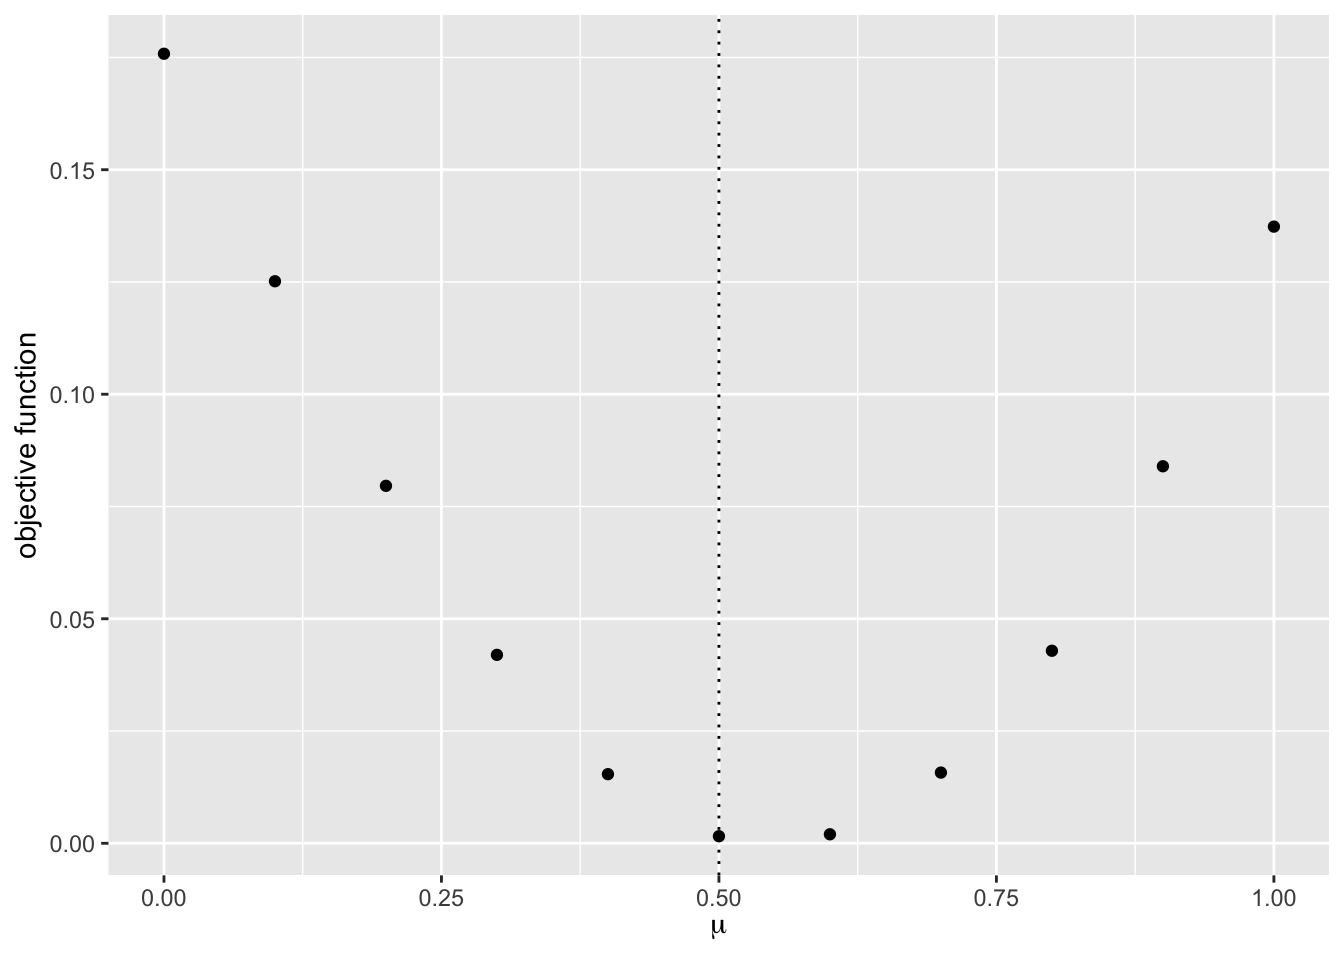
\includegraphics{lecture_files/figure-latex/unnamed-chunk-134-1} \end{center}

\begin{verbatim}
## 
## [[2]]
\end{verbatim}

\begin{center}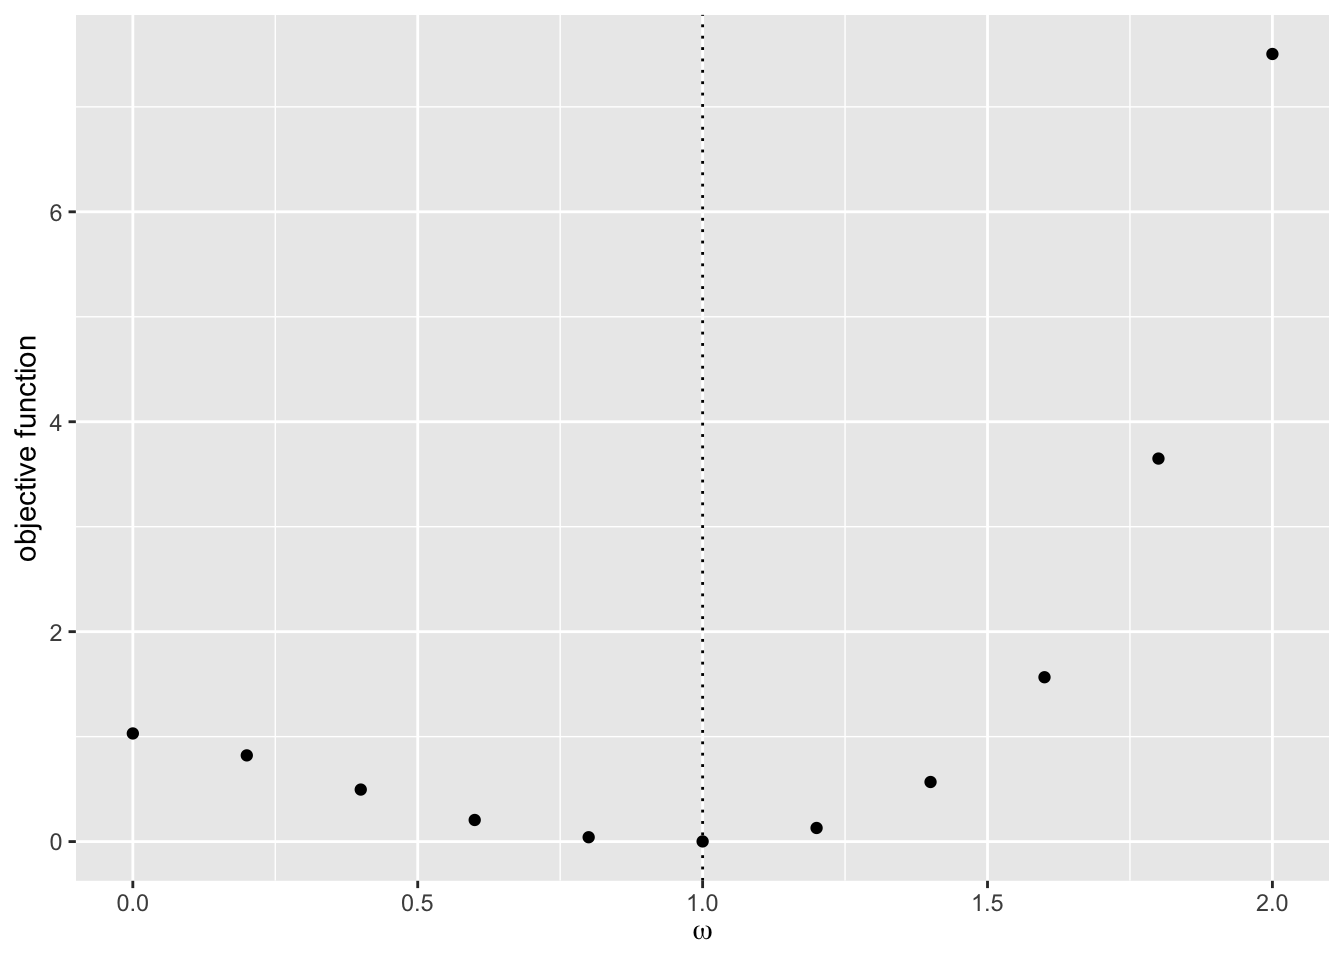
\includegraphics{lecture_files/figure-latex/unnamed-chunk-134-2} \end{center}

\begin{verbatim}
## 
## [[3]]
\end{verbatim}

\begin{center}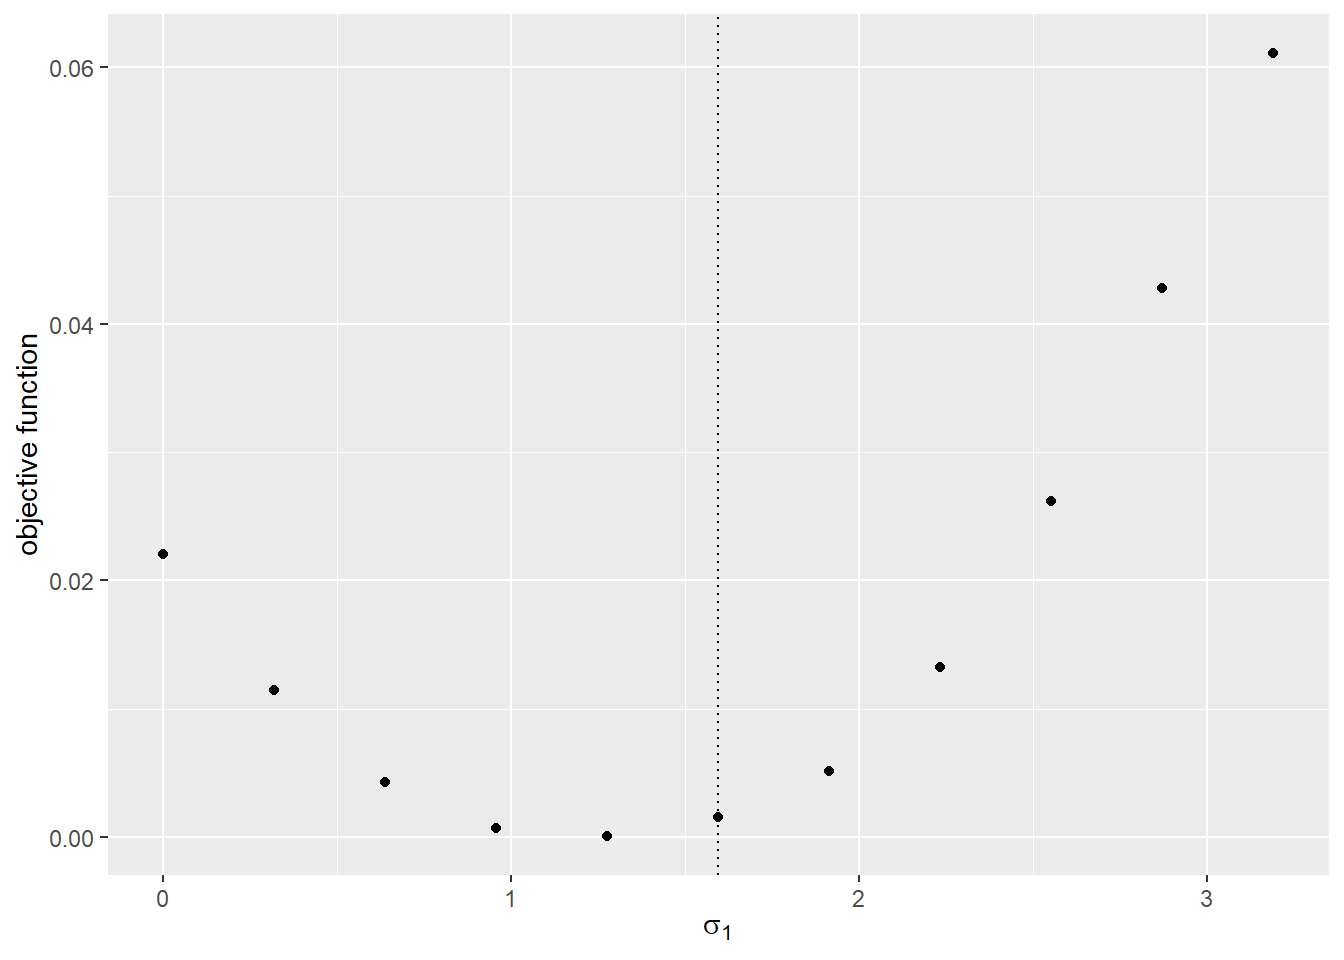
\includegraphics{lecture_files/figure-latex/unnamed-chunk-134-3} \end{center}

\begin{verbatim}
## 
## [[4]]
\end{verbatim}

\begin{center}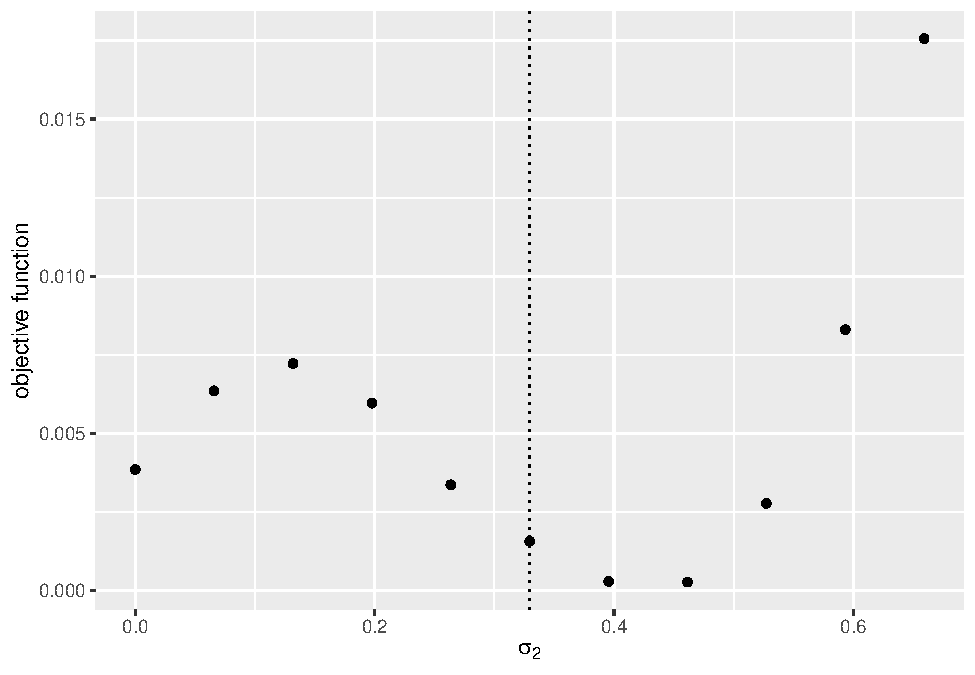
\includegraphics{lecture_files/figure-latex/unnamed-chunk-134-4} \end{center}

\begin{verbatim}
## 
## [[5]]
\end{verbatim}

\begin{center}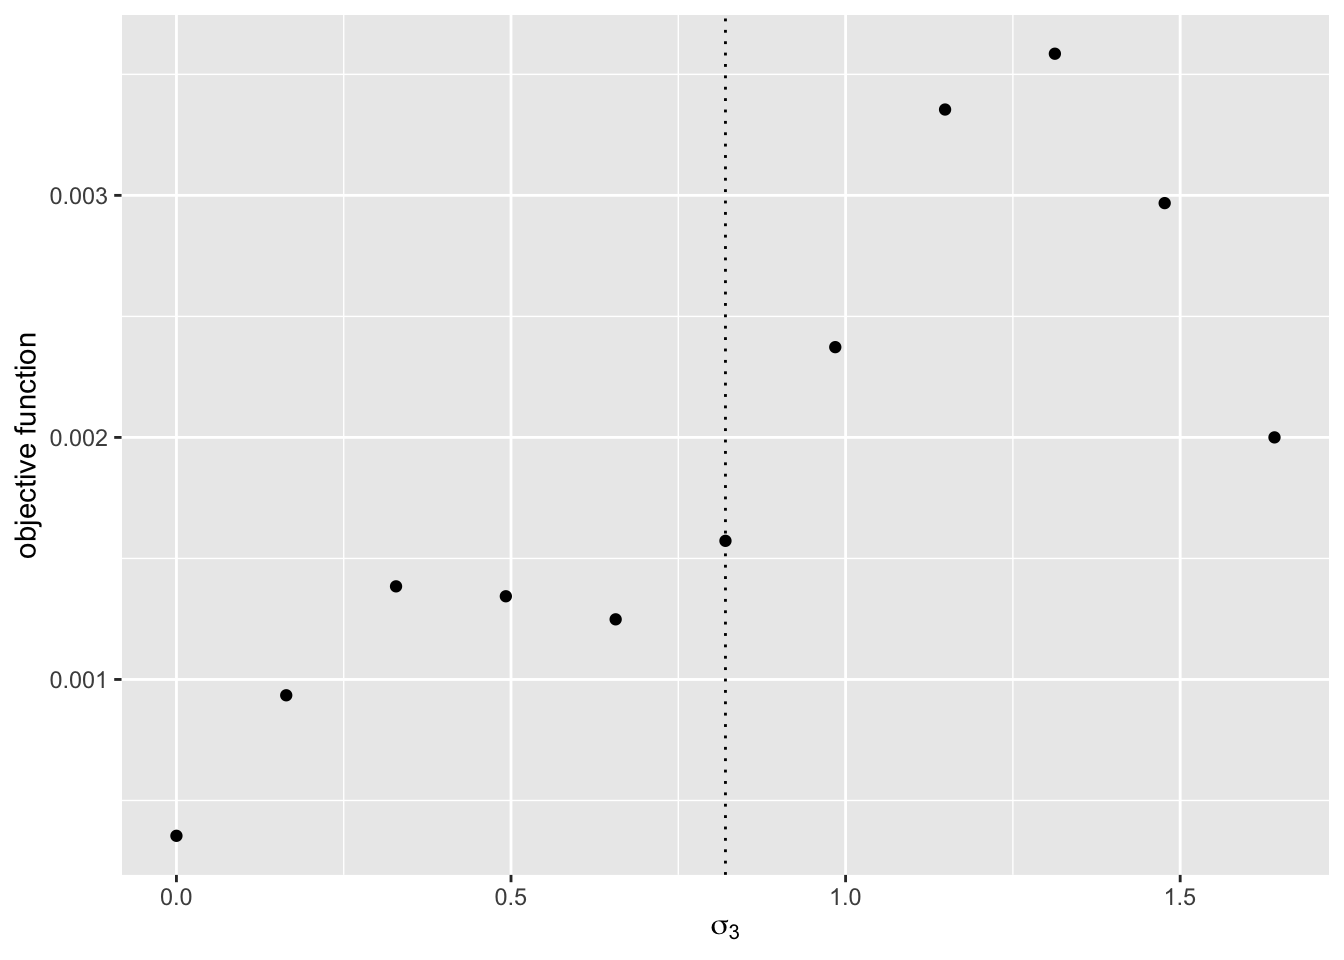
\includegraphics{lecture_files/figure-latex/unnamed-chunk-134-5} \end{center}

\begin{enumerate}
\def\labelenumi{\arabic{enumi}.}
\setcounter{enumi}{12}
\tightlist
\item
  Find non-linear parameters that minimize the GMM objective function.
  Because standard deviations of the same absolute value with positive
  and negative values have almost the same implication for the data, you
  can take the absolute value if the estimates of the standard
  deviations happened to be negative (Another way is to set the
  non-negativity constraints on the standard deviations).
\end{enumerate}

\begin{verbatim}
## $par
## [1] 0.3635051 0.7502512 1.5852184 0.4223104 0.8757237
## 
## $value
## [1] 2.064906e-18
## 
## $counts
## function gradient 
##       54       11 
## 
## $convergence
## [1] 0
## 
## $message
## NULL
\end{verbatim}

\begin{verbatim}
##           true  estimate
## [1,] 0.5000000 0.3635051
## [2,] 1.0000000 0.7502512
## [3,] 1.5952808 1.5852184
## [4,] 0.3295078 0.4223104
## [5,] 0.8204684 0.8757237
\end{verbatim}

\chapter{Integrating with C++ using Rcpp and RcppEigen}\label{rcpp}

\section{Prerequisite}\label{prerequisite}

\begin{itemize}
\item
  In this chapter, we learn how to integrate C++ using Rcpp and
  RcppEigen.
\item
  \texttt{RcppEigen} is a package to use a linear algebra library
  \texttt{Eigen} with R. The original \texttt{Eigen} library and its
  documentation is found in
  \href{http://eigen.tuxfamily.org/index.php?title=Main_Page}{their
  website}.
\item
  Instead of \texttt{RcppEigen}, you may want to use
  \texttt{RcppArmadillo}. \texttt{Armadillo} is another libear algebra
  library in C++.
\item
  We presume that:

  \begin{itemize}
  \tightlist
  \item
    C/C++ environment is installed to the computer.

    \begin{itemize}
    \tightlist
    \item
      For OSX, you can install
      \href{https://developer.apple.com/xcode/}{Apple Developer Tools}.
    \item
      For Windows, you can try
      \href{https://cran.r-project.org/bin/windows/Rtools/}{Rtools}.
    \end{itemize}
  \item
    \texttt{Rcpp} and \texttt{RcppEigen} are installed.
  \item
    The project is created in RStudio from
    \texttt{File\ \textgreater{}\ New\ Project\ \textgreater{}\ New\ Directory\ \textgreater{}\ R\ Package\ using\ RcppEigen}.
    In the following, I use the project name \texttt{EmpiricalIO} but
    the name can be as you like.
  \end{itemize}
\item
  We presume the you have the following folder and file structure from
  the root directory:

  \begin{itemize}
  \tightlist
  \item
    \texttt{main}.

    \begin{itemize}
    \tightlist
    \item
      \texttt{main.R}: all executable statements are written in this
      file.
    \end{itemize}
  \item
    \texttt{R}.

    \begin{itemize}
    \tightlist
    \item
      \texttt{functions.R}: all function definitions in R are written in
      this file.
    \end{itemize}
  \item
    \texttt{src}.

    \begin{itemize}
    \tightlist
    \item
      \texttt{functions.cpp}: all function definitions in C++ are
      written in this file.

      \begin{itemize}
      \item
        It includes:

\begin{verbatim}
"src/functions.cpp"
-------------------
#include <Rcpp.h>
#include <RcppEigen.h>
\end{verbatim}
      \end{itemize}
    \item
      Inside \texttt{functions.cpp}, avoid using name spaces.
    \item
      \texttt{Makevars}: compilation flags for osx/Linux should be
      written here.
    \item
      \texttt{Makevars.win}: compilation flags for Windows should be
      written here.
    \end{itemize}
  \item
    \texttt{inst}.

    \begin{itemize}
    \tightlist
    \item
      \texttt{include}: header files for external libraries in C/C++ are
      stored here.
    \end{itemize}
  \end{itemize}
\item
  \texttt{Makevars/Makevars.win} should be:

\begin{verbatim}
Makevars
--------
PKG_CPPFLAGS = -w -std=c++11 -I../inst/include/ -O3
\end{verbatim}

\begin{verbatim}
Makevars.win
------------
PKG_CPPFLAGS = -w -std=c++11 -I../inst/include/ -O3
\end{verbatim}

  \begin{itemize}
  \tightlist
  \item
    \texttt{-w} is for supprssing some warnings in \texttt{Eigen}. If
    you want to keep warnings shown, this can be removed.
  \item
    \texttt{-std=c++11} is for using the latest functionalities of C++
    (optional).
  \item
    \texttt{-I../inst/include/} is for setting the header path to
    \texttt{../inst/include/} (optional).
  \end{itemize}
\end{itemize}

\section{Workflow}\label{workflow}

\begin{itemize}
\tightlist
\item
  To minimize the likelihood of bugs and the time to edit and debug the
  code, I recommend you to follw the following workflow.
\item
  This workflow is based on my experience. If you find better workflow,
  you can overwrite by your own way.
\end{itemize}

\begin{enumerate}
\def\labelenumi{\arabic{enumi}.}
\tightlist
\item
  Write a procedure in \texttt{main/main.R}.
\end{enumerate}

\begin{Shaded}
\begin{Highlighting}[]
\CommentTok{# main/main.R}
\NormalTok{x <-}\StringTok{ }\DecValTok{1}\OperatorTok{:}\DecValTok{4}
\NormalTok{y1 <-}\StringTok{ }\NormalTok{x}\OperatorTok{^}\DecValTok{2}
\end{Highlighting}
\end{Shaded}

\begin{enumerate}
\def\labelenumi{\arabic{enumi}.}
\setcounter{enumi}{1}
\tightlist
\item
  Rewrite the procedure to a function in \texttt{main/main.R}.
\end{enumerate}

\begin{Shaded}
\begin{Highlighting}[]
\CommentTok{# main/main.R}
\CommentTok{# compute coefficient-wise square}
\NormalTok{compute_square <-}
\StringTok{  }\ControlFlowTok{function}\NormalTok{(x) \{}
\NormalTok{    y <-}\StringTok{ }\NormalTok{x}\OperatorTok{^}\DecValTok{2}
    \KeywordTok{return}\NormalTok{(y)}
\NormalTok{  \}}
\end{Highlighting}
\end{Shaded}

\begin{enumerate}
\def\labelenumi{\arabic{enumi}.}
\setcounter{enumi}{2}
\tightlist
\item
  Execute the function in \texttt{main/main.R} and check that the output
  is the same with the output of the original
\end{enumerate}

\begin{Shaded}
\begin{Highlighting}[]
\CommentTok{# main/main.R}
\NormalTok{y2 <-}\StringTok{ }\KeywordTok{compute_square}\NormalTok{(x)}
\KeywordTok{max}\NormalTok{(}\KeywordTok{abs}\NormalTok{(y1 }\OperatorTok{-}\StringTok{ }\NormalTok{y2))}
\end{Highlighting}
\end{Shaded}

\begin{verbatim}
## [1] 0
\end{verbatim}

\begin{enumerate}
\def\labelenumi{\arabic{enumi}.}
\setcounter{enumi}{3}
\item
  Cut and paste the function to \texttt{R/functions.R}.
\item
  Build the package and load the function from the library.
\item
  Check if the function can be executed as in step 3.
\item
  Copy the function to \texttt{src/functions.cpp} and comment them out.

\begin{verbatim}
// src/functions.cpp
// # compute coefficient-wise square
// compute_square <-
//   function(x) {
//     y <- x^2
//     return(y)
//   }
\end{verbatim}
\item
  Write function in C++ by translating the copied and pasted R code.

  \begin{itemize}
  \tightlist
  \item
    The function name should be consistent with the function name in R.
    I often put \texttt{\_rcpp} to the end of the name.
  \item
    Put \texttt{//\ {[}{[}Rcpp::export{]}{]}} above the name of the
    function if you want to call this function directly from R.
    Otherwise, the wrapper function to call from R is not created.
  \item
    The class of the inputs and output should be consistent with
    \texttt{Rcpp} objects. This will be explained later.
  \end{itemize}
\end{enumerate}

\begin{verbatim}
// src/functions.cpp
// # compute coefficient-wise square
// compute_square <-
// [[Rcpp::export]]
Eigen::VectorXd compute_square_rcpp(Eigen::VectorXd x) {
  //   function(x) {
  Eigen::VectorXd y = x.array().square();
  //     y <- x^2
  //     return(y)
  //   }
  return(y);
}
\end{verbatim}

\begin{enumerate}
\def\labelenumi{\arabic{enumi}.}
\setcounter{enumi}{8}
\tightlist
\item
  Check if clean and rebuild work.

  \begin{itemize}
  \tightlist
  \item
    If there is a compilation error happens, debug until the compilation
    succeeds.
  \item
    Sometimes, deleting \texttt{R/RcppExports.R} and
    \texttt{R/RcppExports.cpp} may be need when re-compile the
    functions.
  \end{itemize}
\item
  Clean up the code by eliminating the copied and pasted R code.
\end{enumerate}

\begin{verbatim}
// src/functions.cpp
// compute coefficient-wise square
// [[Rcpp::export]]
Eigen::VectorXd compute_square_rcpp(Eigen::VectorXd x) {
  Eigen::VectorXd y = x.array().square();
  return(y);
}
\end{verbatim}

\begin{enumerate}
\def\labelenumi{\arabic{enumi}.}
\setcounter{enumi}{10}
\tightlist
\item
  Now by calling the library, you should be able to use the function
  written in C++ in R. Check if it returns a valid value and if the
  output is the same as the output of the R function.
\end{enumerate}

\begin{Shaded}
\begin{Highlighting}[]
\CommentTok{# main/main.R}
\NormalTok{y3 <-}\StringTok{ }\KeywordTok{compute_square_rcpp}\NormalTok{(x)}
\KeywordTok{max}\NormalTok{(}\KeywordTok{abs}\NormalTok{(y2 }\OperatorTok{-}\StringTok{ }\NormalTok{y3))}
\end{Highlighting}
\end{Shaded}

\begin{verbatim}
## [1] 0
\end{verbatim}

\begin{enumerate}
\def\labelenumi{\arabic{enumi}.}
\setcounter{enumi}{11}
\tightlist
\item
  If there is a run-time bug in the C++ function, you may have to use
  some debugger for C++ to debug the function.

  \begin{itemize}
  \item
    In osx, you can debug the C++ function called from R function in the
    following way.
  \item
    Open the terminal and run R with the debugger \texttt{lldb} by
    typing the following command in the terminal:

\begin{verbatim}
# terminal
R -d lldb
\end{verbatim}
  \item
    Run \texttt{main/main.R} by typing the following command in the
    terminal:

\begin{verbatim}
# terminal
run -f main/main.R
\end{verbatim}
  \item
    This should execute the R source code.
  \item
    After \texttt{library(EmpiricalIO)} is read, stop the process by
    \texttt{Ctrl\ +\ C} before the function in question is called. If
    there is no time gap between them, set \texttt{Sys.sleep()} in R to
    buy some time.
  \item
    As you stop the process, set the break point at the function in
    question by typing in the terminal as:

\begin{verbatim}
# terminal
br s -n compute_square_rcpp
\end{verbatim}

    and then continue the process by typing \texttt{c} in the terminal.
  \item
    For the rest, refer to the
    \href{https://lldb.llvm.org/}{documentation of lldb}.
  \item
    There is no such an easy way in Windows. You will have to establish
    an environment in which you can run a cpp file with executable
    statemtns and call the debugging functions from the file. Then, you
    can use some debuggers such as \texttt{gdb} to debug the functions
    inside the cpp file.
  \end{itemize}
\item
  If you need to modify the function, first rewrite the R function and
  then follow the same step to rewrite the C++ function. Never start the
  debugging from C++ functions.
\end{enumerate}

\section{Passing R Objects as Rcpp
Objects}\label{passing-r-objects-as-rcpp-objects}

\begin{itemize}
\tightlist
\item
  R class corresponds to the following Rcpp class:
\end{itemize}

\begin{longtable}[]{@{}ll@{}}
\toprule
R & Rcpp\tabularnewline
\midrule
\endhead
\texttt{logical} & \texttt{Logical}\tabularnewline
\texttt{integer} & \texttt{Integer}\tabularnewline
\texttt{numeric} & \texttt{Numeric}\tabularnewline
\texttt{complex} & \texttt{Complex}\tabularnewline
\texttt{character} & \texttt{String}\tabularnewline
\texttt{Date} & \texttt{Date}\tabularnewline
\texttt{POSIXct} & \texttt{Datetime}\tabularnewline
\bottomrule
\end{longtable}

\begin{itemize}
\tightlist
\item
  R data structure corresponds to the following Rcpp data structure:
\end{itemize}

\begin{longtable}[]{@{}ll@{}}
\toprule
R & Rcpp\tabularnewline
\midrule
\endhead
\texttt{vector} & \texttt{Vector}\tabularnewline
\texttt{matrix} & \texttt{Matrix}\tabularnewline
\texttt{data.frame} & \texttt{DataFrame}\tabularnewline
\texttt{list} & \texttt{List}\tabularnewline
\bottomrule
\end{longtable}

\begin{itemize}
\tightlist
\item
  For example, a numeric vector in R is passed to
  \texttt{Rcpp::NumericVector} in Rcpp, an integer matrix is to
  \texttt{Rcpp::IntegerMatrix}, and so on.
\end{itemize}

\begin{Shaded}
\begin{Highlighting}[]
\CommentTok{# main/main.R}
\CommentTok{# numeric vector }
\NormalTok{x <-}\StringTok{ }\KeywordTok{rnorm}\NormalTok{(}\DecValTok{5}\NormalTok{)}
\NormalTok{x}
\end{Highlighting}
\end{Shaded}

\begin{verbatim}
## [1] -0.9159760  0.2750165 -1.4173615  1.5778831 -2.1781476
\end{verbatim}

\begin{Shaded}
\begin{Highlighting}[]
\CommentTok{# numeric matrix}
\NormalTok{Y <-}\StringTok{ }\KeywordTok{matrix}\NormalTok{(}\KeywordTok{rnorm}\NormalTok{(}\DecValTok{2}\OperatorTok{*}\DecValTok{5}\NormalTok{), }\DataTypeTok{nrow =} \DecValTok{2}\NormalTok{)}
\NormalTok{Y}
\end{Highlighting}
\end{Shaded}

\begin{verbatim}
##            [,1]      [,2]        [,3]       [,4]       [,5]
## [1,] -1.0509051 0.9240679  0.01461874 -0.1573930 -0.1157289
## [2,] -0.4767702 0.4508252 -0.25871885 -0.4637887  0.8536339
\end{verbatim}

\begin{itemize}
\tightlist
\item
  Let's write a C++ function that just receives a numeric vector and
  returns the numeric vector, and receives a numeric matrix and returns
  the numeric matrix.
\end{itemize}

\begin{verbatim}
// src/functions.cpp
// [[Rcpp::export]]
Rcpp::NumericVector pass_numeric_vector_to_rcpp(Rcpp::NumericVector x) {
  return(x);
}
// [[Rcpp::export]]
Rcpp::NumericMatrix pass_numeric_matrix_to_rcpp(Rcpp::NumericMatrix Y) {
  return(Y);
}
\end{verbatim}

\begin{itemize}
\tightlist
\item
  Check if you can pass R objects and get the right result:
\end{itemize}

\begin{Shaded}
\begin{Highlighting}[]
\CommentTok{# main/main.r}
\NormalTok{x_rcpp <-}\StringTok{ }\KeywordTok{pass_numeric_vector_to_rcpp}\NormalTok{(x)}
\KeywordTok{max}\NormalTok{(}\KeywordTok{abs}\NormalTok{(x }\OperatorTok{-}\StringTok{ }\NormalTok{x_rcpp))}
\end{Highlighting}
\end{Shaded}

\begin{verbatim}
## [1] 0
\end{verbatim}

\begin{Shaded}
\begin{Highlighting}[]
\NormalTok{Y_rcpp <-}\StringTok{ }\KeywordTok{pass_numeric_matrix_to_rcpp}\NormalTok{(Y)}
\KeywordTok{max}\NormalTok{(}\KeywordTok{abs}\NormalTok{(Y }\OperatorTok{-}\StringTok{ }\NormalTok{Y_rcpp))}
\end{Highlighting}
\end{Shaded}

\begin{verbatim}
## [1] 0
\end{verbatim}

\begin{itemize}
\tightlist
\item
  \textbf{Exercise}: Write functions
  \texttt{pass\_integer\_vector\_to\_rcpp},
  \texttt{pass\_integer\_matrix\_to\_rcpp},
  \texttt{pass\_list\_to\_rcpp}, \texttt{pass\_data\_frame\_to\_rcpp}
  that receive an integer vector, list, and data frame and just return
  themselves.
\end{itemize}

\begin{Shaded}
\begin{Highlighting}[]
\CommentTok{# main/main.r}
\CommentTok{# integer vector}
\NormalTok{z <-}\StringTok{ }\DecValTok{1}\OperatorTok{:}\DecValTok{5}
\NormalTok{z}
\end{Highlighting}
\end{Shaded}

\begin{verbatim}
## [1] 1 2 3 4 5
\end{verbatim}

\begin{Shaded}
\begin{Highlighting}[]
\CommentTok{# integer matrix}
\NormalTok{W <-}\StringTok{ }\KeywordTok{matrix}\NormalTok{(}\KeywordTok{rep}\NormalTok{(}\DecValTok{1}\NormalTok{, }\DecValTok{4}\NormalTok{), }\DataTypeTok{nrow =} \DecValTok{2}\NormalTok{)}
\NormalTok{W}
\end{Highlighting}
\end{Shaded}

\begin{verbatim}
##      [,1] [,2]
## [1,]    1    1
## [2,]    1    1
\end{verbatim}

\begin{Shaded}
\begin{Highlighting}[]
\CommentTok{# list}
\NormalTok{L <-}\StringTok{ }\KeywordTok{list}\NormalTok{(}\DataTypeTok{x =}\NormalTok{ x, }\DataTypeTok{y =}\NormalTok{ y, }\DataTypeTok{z =}\NormalTok{ z)}
\NormalTok{L}
\end{Highlighting}
\end{Shaded}

\begin{verbatim}
## $x
## [1] -0.9159760  0.2750165 -1.4173615  1.5778831 -2.1781476
## 
## $y
## [1] 1
## 
## $z
## [1] 1 2 3 4 5
\end{verbatim}

\begin{Shaded}
\begin{Highlighting}[]
\CommentTok{# data frame}
\NormalTok{D <-}\StringTok{ }\KeywordTok{data.frame}\NormalTok{(}\DataTypeTok{x1 =} \KeywordTok{rnorm}\NormalTok{(}\DecValTok{5}\NormalTok{), }\DataTypeTok{x2 =} \KeywordTok{rnorm}\NormalTok{(}\DecValTok{5}\NormalTok{))}
\NormalTok{D}
\end{Highlighting}
\end{Shaded}

\begin{verbatim}
##            x1          x2
## 1 -0.86280066 -1.03184291
## 2 -1.15758053  0.77688232
## 3 -0.89268670  0.21788910
## 4  0.04043654  1.33717072
## 5  2.25861844 -0.07430342
\end{verbatim}

\begin{Shaded}
\begin{Highlighting}[]
\NormalTok{z_rcpp <-}\StringTok{ }\KeywordTok{pass_integer_vector_to_rcpp}\NormalTok{(z)}
\KeywordTok{max}\NormalTok{(}\KeywordTok{abs}\NormalTok{(z }\OperatorTok{-}\StringTok{ }\NormalTok{z_rcpp))}
\end{Highlighting}
\end{Shaded}

\begin{verbatim}
## [1] 0
\end{verbatim}

\begin{Shaded}
\begin{Highlighting}[]
\NormalTok{W_rcpp <-}\StringTok{ }\KeywordTok{pass_integer_matrix_to_rcpp}\NormalTok{(W)}
\KeywordTok{max}\NormalTok{(}\KeywordTok{abs}\NormalTok{(W }\OperatorTok{-}\StringTok{ }\NormalTok{W_rcpp))}
\end{Highlighting}
\end{Shaded}

\begin{verbatim}
## [1] 0
\end{verbatim}

\begin{Shaded}
\begin{Highlighting}[]
\NormalTok{L_rcpp <-}\StringTok{ }\KeywordTok{pass_list_to_rcpp}\NormalTok{(L)}
\KeywordTok{max}\NormalTok{(}\KeywordTok{abs}\NormalTok{(}\KeywordTok{unlist}\NormalTok{(L) }\OperatorTok{-}\StringTok{ }\KeywordTok{unlist}\NormalTok{(L_rcpp)))}
\end{Highlighting}
\end{Shaded}

\begin{verbatim}
## [1] 0
\end{verbatim}

\begin{Shaded}
\begin{Highlighting}[]
\NormalTok{D_rcpp <-}\StringTok{ }\KeywordTok{pass_data_frame_to_rcpp}\NormalTok{(D)}
\KeywordTok{max}\NormalTok{(}\KeywordTok{abs}\NormalTok{(D }\OperatorTok{-}\StringTok{ }\NormalTok{D_rcpp))}
\end{Highlighting}
\end{Shaded}

\begin{verbatim}
## [1] 0
\end{verbatim}

\section{Passing R Objects as Eigen
Objects}\label{passing-r-objects-as-eigen-objects}

\begin{itemize}
\tightlist
\item
  R data structure corresponds to the following Eigen data structure:
\end{itemize}

\begin{longtable}[]{@{}ll@{}}
\toprule
R & Eigen\tabularnewline
\midrule
\endhead
\texttt{vector} & \texttt{Eigen::VectorX}\tabularnewline
\texttt{matrix} & \texttt{Eigen::MatrixX}\tabularnewline
\bottomrule
\end{longtable}

\begin{itemize}
\tightlist
\item
  If you pass an \texttt{integer} vector and matrix, the corresponding
  Eigen objects are \texttt{Eigen::VectorXi} and
  \texttt{Eigen::MatrixXi}.
\item
  If you pass an \texttt{numeric} vector and matrix, the corresponding
  Eigen objects are \texttt{Eigen::VectorXd} and
  \texttt{Eigen::MatrixXd}.
\item
  The class of the output can be Eigen class. If you return
  \texttt{Eigen::VectorXd}, \texttt{Eigen::MatrixXd}, then they are
  automatically converted to the corresponding R objects.
\item
  Check if you can pass \texttt{x}, \texttt{Y}, and \texttt{z} as
  follows:
\end{itemize}

\begin{verbatim}
// src/functions.cpp
// [[Rcpp::export]]
Eigen::VectorXd pass_numeric_vector_to_eigen(Eigen::VectorXd x) {
  return(x);
}
// [[Rcpp::export]]
Eigen::MatrixXd pass_numeric_matrix_to_eigen(Eigen::MatrixXd Y) {
  return(Y);
}
\end{verbatim}

\begin{Shaded}
\begin{Highlighting}[]
\CommentTok{# main/main.r}
\NormalTok{x_eigen <-}\StringTok{ }\KeywordTok{pass_numeric_vector_to_eigen}\NormalTok{(x)}
\KeywordTok{max}\NormalTok{(}\KeywordTok{abs}\NormalTok{(x }\OperatorTok{-}\StringTok{ }\NormalTok{x_eigen))}
\end{Highlighting}
\end{Shaded}

\begin{verbatim}
## [1] 0
\end{verbatim}

\begin{Shaded}
\begin{Highlighting}[]
\NormalTok{Y_eigen <-}\StringTok{ }\KeywordTok{pass_numeric_matrix_to_eigen}\NormalTok{(Y)}
\KeywordTok{max}\NormalTok{(}\KeywordTok{abs}\NormalTok{(Y }\OperatorTok{-}\StringTok{ }\NormalTok{Y_eigen))}
\end{Highlighting}
\end{Shaded}

\begin{verbatim}
## [1] 0
\end{verbatim}

\begin{itemize}
\tightlist
\item
  \textbf{Exercise}: Write functions
  \texttt{pass\_integer\_vector\_to\_rcpp} and
  \texttt{pass\_integer\_matrix\_to\_rcpp} that receive an integer
  vector and integer matrix and just return themselves.
\end{itemize}

\begin{Shaded}
\begin{Highlighting}[]
\CommentTok{# main/main.r}
\NormalTok{z_eigen <-}\StringTok{ }\KeywordTok{pass_integer_vector_to_eigen}\NormalTok{(z)}
\KeywordTok{max}\NormalTok{(}\KeywordTok{abs}\NormalTok{(z }\OperatorTok{-}\StringTok{ }\NormalTok{z_eigen))}
\end{Highlighting}
\end{Shaded}

\begin{verbatim}
## [1] 0
\end{verbatim}

\begin{Shaded}
\begin{Highlighting}[]
\NormalTok{W_eigen <-}\StringTok{ }\KeywordTok{pass_integer_matrix_to_eigen}\NormalTok{(W)}
\KeywordTok{max}\NormalTok{(}\KeywordTok{abs}\NormalTok{(W }\OperatorTok{-}\StringTok{ }\NormalTok{W_eigen))}
\end{Highlighting}
\end{Shaded}

\begin{verbatim}
## [1] 0
\end{verbatim}

\begin{itemize}
\tightlist
\item
  If you pass a vector and matrix by \texttt{Eigen::VectorX} and
  \texttt{Eigen::MatrixX}, the objects are \textbf{copied} to the new
  objects. This means that the new memory is allocated. If you are going
  to modify the passed object inside the C++ function, the objects have
  to be copied. Otherwise, you can just map the objects in the following
  way so that the new memory is not allocated, whereas you cannot modify
  the objects in the C++ function.
\end{itemize}

\begin{verbatim}
// src/functions.cpp
// [[Rcpp::export]]
Eigen::VectorXd map_numeric_vector_to_eigen(Eigen::Map<Eigen::VectorXd> x) {
  return(x);
}
// [[Rcpp::export]]
Eigen::MatrixXd map_numeric_matrix_to_eigen(Eigen::Map<Eigen::MatrixXd> Y) {
  return(Y);
}
\end{verbatim}

\begin{Shaded}
\begin{Highlighting}[]
\CommentTok{# main/main.r}
\NormalTok{x_eigen_map <-}\StringTok{ }\KeywordTok{map_numeric_vector_to_eigen}\NormalTok{(x)}
\KeywordTok{max}\NormalTok{(}\KeywordTok{abs}\NormalTok{(x }\OperatorTok{-}\StringTok{ }\NormalTok{x_eigen_map))}
\end{Highlighting}
\end{Shaded}

\begin{verbatim}
## [1] 0
\end{verbatim}

\begin{Shaded}
\begin{Highlighting}[]
\NormalTok{Y_eigen_map <-}\StringTok{ }\KeywordTok{map_numeric_matrix_to_eigen}\NormalTok{(Y)}
\KeywordTok{max}\NormalTok{(}\KeywordTok{abs}\NormalTok{(Y }\OperatorTok{-}\StringTok{ }\NormalTok{Y_eigen_map))}
\end{Highlighting}
\end{Shaded}

\begin{verbatim}
## [1] 0
\end{verbatim}

\begin{itemize}
\item
  I recommend to directly pass R vectors and matrices to
  \texttt{Eigen::VectorX} and \texttt{Eigen::MatrixX} rather than to
  \texttt{Vector} and \texttt{Matrix} in Rcpp, because
  \texttt{Eigen::VectorX} and \texttt{Eigen::MatrixX} have richer
  methods for linear algebra.
\item
  R list cannot be directly translated to Eigen objects, but the list of
  vectors and matrices, and the list of list of R objects can be passed
  to Eigen in the following way.
\end{itemize}

\begin{verbatim}
// src/functions.cpp
// [[Rcpp::export]]
Rcpp::List pass_list_to_eigen(Rcpp::List L) {
  // double vector
  Eigen::VectorXd x(Rcpp::as<Eigen::VectorXd>(L.at(0)));
  // double matrix
  Eigen::MatrixXd Y(Rcpp::as<Eigen::MatrixXd>(L.at(1)));
  // integer vector
  Eigen::VectorXi z(Rcpp::as<Eigen::VectorXi>(L.at(2)));
  // integer matrix
  Eigen::MatrixXi W(Rcpp::as<Eigen::MatrixXi>(L.at(3)));
  // return
  Rcpp::List output = Rcpp::List::create(x, Y, z, W);
  return(output);
}
\end{verbatim}

\begin{Shaded}
\begin{Highlighting}[]
\CommentTok{# main/main.r}
\NormalTok{list_}\DecValTok{1}\NormalTok{ <-}\StringTok{ }\KeywordTok{list}\NormalTok{()}
\NormalTok{list_}\DecValTok{1}\NormalTok{[[}\DecValTok{1}\NormalTok{]] <-}\StringTok{ }\NormalTok{x}
\NormalTok{list_}\DecValTok{1}\NormalTok{[[}\DecValTok{2}\NormalTok{]] <-}\StringTok{ }\NormalTok{Y}
\NormalTok{list_}\DecValTok{1}\NormalTok{[[}\DecValTok{3}\NormalTok{]] <-}\StringTok{ }\NormalTok{z}
\NormalTok{list_}\DecValTok{1}\NormalTok{[[}\DecValTok{4}\NormalTok{]] <-}\StringTok{ }\NormalTok{W}
\NormalTok{list_}\DecValTok{1}
\end{Highlighting}
\end{Shaded}

\begin{verbatim}
## [[1]]
## [1] -0.9159760  0.2750165 -1.4173615  1.5778831 -2.1781476
## 
## [[2]]
##            [,1]      [,2]        [,3]       [,4]       [,5]
## [1,] -1.0509051 0.9240679  0.01461874 -0.1573930 -0.1157289
## [2,] -0.4767702 0.4508252 -0.25871885 -0.4637887  0.8536339
## 
## [[3]]
## [1] 1 2 3 4 5
## 
## [[4]]
##      [,1] [,2]
## [1,]    1    1
## [2,]    1    1
\end{verbatim}

\begin{Shaded}
\begin{Highlighting}[]
\NormalTok{list_1_eigen <-}\StringTok{ }\KeywordTok{pass_list_to_eigen}\NormalTok{(list_}\DecValTok{1}\NormalTok{)}
\KeywordTok{max}\NormalTok{(}\KeywordTok{abs}\NormalTok{(}\KeywordTok{unlist}\NormalTok{(list_}\DecValTok{1}\NormalTok{) }\OperatorTok{-}\StringTok{ }\KeywordTok{unlist}\NormalTok{(list_1_eigen)))}
\end{Highlighting}
\end{Shaded}

\begin{verbatim}
## [1] 0
\end{verbatim}

\begin{itemize}
\tightlist
\item
  You can also pass a list with named arguments and return a named list
  as follows:
\end{itemize}

\begin{verbatim}
// src/funtions.cpp
// [[Rcpp::export]]
Rcpp::List pass_named_list_to_eigen(Rcpp::List L) {
  // double vector
  Eigen::VectorXd x(Rcpp::as<Eigen::VectorXd>(L["x"]));
  // double matrix
  Eigen::MatrixXd Y(Rcpp::as<Eigen::MatrixXd>(L["Y"]));
  // integer vector
  Eigen::VectorXi z(Rcpp::as<Eigen::VectorXi>(L["z"]));
  // integer matrix
  Eigen::MatrixXi W(Rcpp::as<Eigen::MatrixXi>(L["W"]));
  // return
  Rcpp::List output = Rcpp::List::create(
    Rcpp::Named("x") = x, 
    Rcpp::Named("Y") = Y, 
    Rcpp::Named("z") = z, 
    Rcpp::Named("W") = W);
  return(output);
}
\end{verbatim}

\begin{Shaded}
\begin{Highlighting}[]
\CommentTok{# main/main.r}
\NormalTok{list_}\DecValTok{2}\NormalTok{ <-}\StringTok{ }\KeywordTok{list}\NormalTok{()}
\NormalTok{list_}\DecValTok{2}\OperatorTok{$}\NormalTok{x <-}\StringTok{ }\NormalTok{x}
\NormalTok{list_}\DecValTok{2}\OperatorTok{$}\NormalTok{Y <-}\StringTok{ }\NormalTok{Y}
\NormalTok{list_}\DecValTok{2}\OperatorTok{$}\NormalTok{z <-}\StringTok{ }\NormalTok{z}
\NormalTok{list_}\DecValTok{2}\OperatorTok{$}\NormalTok{W <-}\StringTok{ }\NormalTok{W}
\NormalTok{list_}\DecValTok{2}
\end{Highlighting}
\end{Shaded}

\begin{verbatim}
## $x
## [1] -0.9159760  0.2750165 -1.4173615  1.5778831 -2.1781476
## 
## $Y
##            [,1]      [,2]        [,3]       [,4]       [,5]
## [1,] -1.0509051 0.9240679  0.01461874 -0.1573930 -0.1157289
## [2,] -0.4767702 0.4508252 -0.25871885 -0.4637887  0.8536339
## 
## $z
## [1] 1 2 3 4 5
## 
## $W
##      [,1] [,2]
## [1,]    1    1
## [2,]    1    1
\end{verbatim}

\begin{Shaded}
\begin{Highlighting}[]
\NormalTok{list_2_eigen <-}\StringTok{ }\KeywordTok{pass_named_list_to_eigen}\NormalTok{(list_}\DecValTok{2}\NormalTok{)}
\KeywordTok{max}\NormalTok{(}\KeywordTok{abs}\NormalTok{(}\KeywordTok{unlist}\NormalTok{(list_}\DecValTok{2}\NormalTok{) }\OperatorTok{-}\StringTok{ }\KeywordTok{unlist}\NormalTok{(list_2_eigen)))}
\end{Highlighting}
\end{Shaded}

\begin{verbatim}
## [1] 0
\end{verbatim}

\begin{itemize}
\tightlist
\item
  You can also access to the column of \texttt{Rcpp::DataFrame} in the
  similar way.
\end{itemize}

\begin{verbatim}
// src/functions.cpp
// [[Rcpp::export]]
Eigen::VectorXd extract_column_from_data_frame(Rcpp::DataFrame D) {
  // pass column x1 of D to Eigen::VectorXd named x1
  Eigen::VectorXd x1(Rcpp::as<Eigen::VectorXd>(D["x1"]));
  return(x1);
}
\end{verbatim}

\begin{Shaded}
\begin{Highlighting}[]
\CommentTok{# main/main.R}
\NormalTok{x1 <-}\StringTok{ }\KeywordTok{extract_column_from_data_frame}\NormalTok{(D)}
\KeywordTok{max}\NormalTok{(}\KeywordTok{abs}\NormalTok{(D}\OperatorTok{$}\NormalTok{x1 }\OperatorTok{-}\StringTok{ }\NormalTok{x1))}
\end{Highlighting}
\end{Shaded}

\begin{verbatim}
## [1] 0
\end{verbatim}

\begin{itemize}
\tightlist
\item
  This allows us to pass whatever objects in R to a C++ function.
\item
  If you are planning to translate R functions to C/C++, from the
  beginning, you should write the R functions in the way inputs and
  outpus can be passed to C/C++ as above.
\end{itemize}

\section{Passing R Objects in Other Objects in
C/C++}\label{passing-r-objects-in-other-objects-in-cc}

\begin{itemize}
\tightlist
\item
  \texttt{integer} and \texttt{numeric} scalars in R can be simply
  passed to \texttt{int} and \texttt{double} in C/C++.
\item
  Vectors in R can be passed to
  \texttt{std::vector\textless{}int\textgreater{}} or
  \texttt{std::vector\textless{}double\textgreater{}} objects. This may
  be helpful if you want to use the methods for \texttt{std::vector}.
\end{itemize}

\section{Manipulating Objects in a C++
Function}\label{manipulating-objects-in-a-c-function}

\begin{itemize}
\tightlist
\item
  As mentioned above, the best practice is to pass vectors and matrices
  to \texttt{Eigen::VectorXd}/\texttt{Eigen::VectorXi} and
  \texttt{Eigen::MatrixXd}/\texttt{Eigen::MatrixXi} rather than
  \texttt{Rcpp::NumericVector}/\texttt{Rcpp::IntegerVector} and
  \texttt{Rcpp::NumericMatrix}/\texttt{Rcpp::IntegerMatrix}.
\item
  The other objects will be passed as \texttt{Rcpp::DataFrame} or
  \texttt{Rcpp::List} and at the end converted to
  \texttt{Eigen::VectorXd}/\texttt{Eigen::VectorXi} and
  \texttt{Eigen::MatrixXd}/\texttt{Eigen::MatrixXi} usin
  \texttt{Rcpp::as} as explained above.
\item
  The rest of manipulation will be done using the methods in Eigen. Here
  I introduce basic operations. For the detail, refer to the
  \href{https://eigen.tuxfamily.org/dox/GettingStarted.html}{online
  document of Eigen}.
\end{itemize}

\subsection{Matrix and Vector
Arithmetic}\label{matrix-and-vector-arithmetic}

\begin{itemize}
\tightlist
\item
  Addition and subtraction:

  \begin{itemize}
  \tightlist
  \item
    Binary operator \(+\) as in \texttt{a\ +\ b}.
  \item
    Binary operator \(-\) as in \texttt{a\ -\ b}.
  \item
    Unary operator \(-\) as in \texttt{-\ a}.
  \end{itemize}
\item
  Scalar multiplication and division:

  \begin{itemize}
  \tightlist
  \item
    Binary operator \(\times\) as in \texttt{matrix\ *\ scalar}.
  \item
    Binary operator \(\times\) as in \texttt{scalar\ *\ matrix}.
  \item
    Binary operator \(/\) as in \texttt{matrix\ /\ scalar}.
  \end{itemize}
\item
  Transposition:

  \begin{itemize}
  \tightlist
  \item
    Transposition as in \texttt{matrix.transpose()}.
  \end{itemize}
\item
  Matrix-matrix and matrix-vector multiplication:

  \begin{itemize}
  \tightlist
  \item
    This part is different from R.
  \item
    Matrix multiplication is as in \texttt{A\ *\ B}.
  \item
    Coefficientwise multiplication is explained later but is as in
    \texttt{A.array()\ *\ B.array()}.
  \end{itemize}
\item
  Following the best practice, first write R function for these
  operations in \texttt{R/functions.R} and run in \texttt{main/main.R}:
\end{itemize}

\begin{Shaded}
\begin{Highlighting}[]
\CommentTok{# R/functions.R}
\CommentTok{# matrix and vector arithmetic}
\NormalTok{matrix_vector_arithmetic <-}
\StringTok{  }\ControlFlowTok{function}\NormalTok{(A, B, v, c) \{}
    \CommentTok{# addition and subtraction}
\NormalTok{    X1 <-}\StringTok{ }\NormalTok{A }\OperatorTok{+}\StringTok{ }\NormalTok{B}
\NormalTok{    X2 <-}\StringTok{ }\NormalTok{A }\OperatorTok{-}\StringTok{ }\NormalTok{B}
\NormalTok{    X3 <-}\StringTok{ }\OperatorTok{-}\NormalTok{A}
    \CommentTok{# scalar multiplication and division}
\NormalTok{    X4 <-}\StringTok{ }\NormalTok{A }\OperatorTok{*}\StringTok{ }\NormalTok{c}
\NormalTok{    X5 <-}\StringTok{ }\NormalTok{c }\OperatorTok{*}\StringTok{ }\NormalTok{A}
\NormalTok{    X6 <-}\StringTok{ }\NormalTok{A }\OperatorTok{/}\StringTok{ }\NormalTok{c}
    \CommentTok{# transpose}
\NormalTok{    X7 <-}\StringTok{ }\KeywordTok{t}\NormalTok{(A)}
    \CommentTok{# matrix-matrix and matrix-vector multiplication}
\NormalTok{    X8 <-}\StringTok{ }\NormalTok{A }\OperatorTok\StringTok{ }\KeywordTok{t}\NormalTok{(B)}
\NormalTok{    X9 <-}\StringTok{ }\NormalTok{A }\OperatorTok\StringTok{ }\NormalTok{v}
    \CommentTok{# return}
    \KeywordTok{return}\NormalTok{(}\KeywordTok{list}\NormalTok{(}\DataTypeTok{X1 =}\NormalTok{ X1,}
                \DataTypeTok{X2 =}\NormalTok{ X2,}
                \DataTypeTok{X3 =}\NormalTok{ X3,}
                \DataTypeTok{X4 =}\NormalTok{ X4,}
                \DataTypeTok{X5 =}\NormalTok{ X5,}
                \DataTypeTok{X6 =}\NormalTok{ X6,}
                \DataTypeTok{X7 =}\NormalTok{ X7,}
                \DataTypeTok{X8 =}\NormalTok{ X8,}
                \DataTypeTok{X9 =}\NormalTok{ X9))}
\NormalTok{  \}}
\end{Highlighting}
\end{Shaded}

\begin{Shaded}
\begin{Highlighting}[]
\CommentTok{# main/main.R}
\KeywordTok{set.seed}\NormalTok{(}\DecValTok{1}\NormalTok{)}
\CommentTok{# addition subtraction}
\NormalTok{A <-}\StringTok{ }\KeywordTok{matrix}\NormalTok{(}\KeywordTok{rnorm}\NormalTok{(}\DecValTok{2}\OperatorTok{*}\DecValTok{4}\NormalTok{), }\DataTypeTok{nrow =} \DecValTok{2}\NormalTok{)}
\NormalTok{B <-}\StringTok{ }\KeywordTok{matrix}\NormalTok{(}\KeywordTok{rnorm}\NormalTok{(}\DecValTok{2}\OperatorTok{*}\DecValTok{4}\NormalTok{), }\DataTypeTok{nrow =} \DecValTok{2}\NormalTok{)}
\NormalTok{c <-}\StringTok{ }\DecValTok{3}
\NormalTok{v <-}\StringTok{ }\KeywordTok{matrix}\NormalTok{(}\KeywordTok{rnorm}\NormalTok{(}\DecValTok{4}\NormalTok{), }\DataTypeTok{nrow =} \DecValTok{4}\NormalTok{)}
\NormalTok{output <-}\StringTok{ }\KeywordTok{matrix_vector_arithmetic}\NormalTok{(A, B, v, c)}
\end{Highlighting}
\end{Shaded}

\begin{itemize}
\item
  Next, write these operations in C++ function:

\begin{verbatim}
// src/functions.cpp
// [[Rcpp::export]]
Rcpp::List matrix_vector_arithmetic_rcpp(
Eigen::MatrixXd A, Eigen::MatrixXd B, 
Eigen::VectorXd v, double c) {
  // addition and subtraction
  Eigen::MatrixXd X1 = A + B;
  Eigen::MatrixXd X2 = A - B;
  Eigen::MatrixXd X3 = - A;
  // scalar multiplication and division
  Eigen::MatrixXd X4 = A * c;
  Eigen::MatrixXd X5 = c * A;
  Eigen::MatrixXd X6 = A / c;
  // transpose
  Eigen::MatrixXd X7 = A.transpose();
  // matrix-matrix and matrix-vector multiplication
  Eigen::MatrixXd X8 = A * B.transpose();
  Eigen::VectorXd X9 = A * v;
  // return 
  Rcpp::List output = 
Rcpp::List::create(
  Rcpp::Named("X1") = X1,
  Rcpp::Named("X2") = X2,
  Rcpp::Named("X3") = X3,
  Rcpp::Named("X4") = X4,
  Rcpp::Named("X5") = X5,
  Rcpp::Named("X6") = X6,
  Rcpp::Named("X7") = X7,
  Rcpp::Named("X8") = X8,
  Rcpp::Named("X9") = X9);
  return(output);
}
\end{verbatim}
\item
  Then, we can check if this yields (almost) the same result with the R
  function:
\end{itemize}

\begin{Shaded}
\begin{Highlighting}[]
\CommentTok{# main/main.R}
\NormalTok{output_rcpp <-}\StringTok{ }\KeywordTok{matrix_vector_arithmetic_rcpp}\NormalTok{(A, B, v, c)}
\KeywordTok{max}\NormalTok{(}\KeywordTok{abs}\NormalTok{(}\KeywordTok{unlist}\NormalTok{(output) }\OperatorTok{-}\StringTok{ }\KeywordTok{unlist}\NormalTok{(output_rcpp)))}
\end{Highlighting}
\end{Shaded}

\begin{verbatim}
## [1] 5.551115e-17
\end{verbatim}

\begin{itemize}
\tightlist
\item
  The output looks like:
\end{itemize}

\begin{Shaded}
\begin{Highlighting}[]
\CommentTok{# main/main.R}
\NormalTok{output_rcpp}
\end{Highlighting}
\end{Shaded}

\begin{verbatim}
## $X1
##             [,1]      [,2]       [,3]      [,4]
## [1,] -0.05067246 0.6761526 -0.2917328 1.6123600
## [2,] -0.12174506 1.9851240 -3.0351683 0.6933911
## 
## $X2
##            [,1]      [,2]      [,3]       [,4]
## [1,] -1.2022352 -2.347410 0.9507484 -0.6375019
## [2,]  0.4890317  1.205438 1.3942315  0.7832583
## 
## $X3
##            [,1]       [,2]       [,3]       [,4]
## [1,]  0.6264538  0.8356286 -0.3295078 -0.4874291
## [2,] -0.1836433 -1.5952808  0.8204684 -0.7383247
## 
## $X4
##           [,1]      [,2]       [,3]     [,4]
## [1,] -1.879361 -2.506886  0.9885233 1.462287
## [2,]  0.550930  4.785842 -2.4614052 2.214974
## 
## $X5
##           [,1]      [,2]       [,3]     [,4]
## [1,] -1.879361 -2.506886  0.9885233 1.462287
## [2,]  0.550930  4.785842 -2.4614052 2.214974
## 
## $X6
##             [,1]       [,2]       [,3]      [,4]
## [1,] -0.20881794 -0.2785429  0.1098359 0.1624764
## [2,]  0.06121444  0.5317603 -0.2734895 0.2461082
## 
## $X7
##            [,1]       [,2]
## [1,] -0.6264538  0.1836433
## [2,] -0.8356286  1.5952808
## [3,]  0.3295078 -0.8204684
## [4,]  0.4874291  0.7383247
## 
## $X8
##           [,1]       [,2]
## [1,] -1.280368 -0.8861152
## [2,]  3.857726  2.3497425
## 
## $X9
## [1] -0.2184706  1.2674165
\end{verbatim}

\subsection{The Array Class and Coefficient-wise
Operations}\label{the-array-class-and-coefficient-wise-operations}

\begin{itemize}
\item
  When you want to have coefficient-wise operations, you first use
  \texttt{.array()} method to convert the object to an array and then
  apply methods for arrays.
\item
  The resulting array can be assigned to a matrix object implicitly or
  explicitly by using \texttt{.matrix()} method.
\item
  Coefficient-wise multiplication:

  \begin{itemize}
  \tightlist
  \item
    \texttt{A\ *\ B} in R is \texttt{A.array()\ *\ B.\ array()} in
    Eigen.
  \end{itemize}
\item
  Other coefficient-wise math functions:

  \begin{itemize}
  \tightlist
  \item
    Absolute value: \texttt{A.array().abs()}.
  \item
    Exponential: \texttt{A.array().exp()}.
  \item
    Logarithm: \texttt{A.array().log()}.
  \item
    Power: \texttt{A.array().power(r)}.
  \item
    For the other methods, refer to the
    \href{https://eigen.tuxfamily.org/dox/group__CoeffwiseMathFunctions.html}{online
    document}.
  \end{itemize}
\item
  Write functions in R in \texttt{R/functions.R} and run in
  \texttt{main/main.R}:
\end{itemize}

\begin{Shaded}
\begin{Highlighting}[]
\CommentTok{# R/functions.R}
\NormalTok{coefficientwise_operation <-}
\StringTok{  }\ControlFlowTok{function}\NormalTok{(A, B, r) \{}
    \CommentTok{# coefficient-wise multiplication}
\NormalTok{    X1 <-}\StringTok{ }\NormalTok{A }\OperatorTok{*}\StringTok{ }\NormalTok{B}
    \CommentTok{# other coefficient-wise math functions}
\NormalTok{    X2 <-}\StringTok{ }\KeywordTok{abs}\NormalTok{(A)}
\NormalTok{    X3 <-}\StringTok{ }\KeywordTok{exp}\NormalTok{(A)}
\NormalTok{    X4 <-}\StringTok{ }\KeywordTok{log}\NormalTok{(}\KeywordTok{abs}\NormalTok{(A))}
\NormalTok{    X5 <-}\StringTok{ }\NormalTok{A}\OperatorTok{^}\NormalTok{r}
    \CommentTok{# return}
    \KeywordTok{return}\NormalTok{(}\KeywordTok{list}\NormalTok{(}
      \DataTypeTok{X1 =}\NormalTok{ X1,}
      \DataTypeTok{X2 =}\NormalTok{ X2,}
      \DataTypeTok{X3 =}\NormalTok{ X3,}
      \DataTypeTok{X4 =}\NormalTok{ X4,}
      \DataTypeTok{X5 =}\NormalTok{ X5}
\NormalTok{    ))}
\NormalTok{  \}}
\end{Highlighting}
\end{Shaded}

\begin{Shaded}
\begin{Highlighting}[]
\CommentTok{# main/main.R}
\CommentTok{# coefficient-wise operations}
\NormalTok{r <-}\StringTok{ }\DecValTok{2}
\NormalTok{output <-}\StringTok{ }\KeywordTok{coefficientwise_operation}\NormalTok{(A, B, r)}
\end{Highlighting}
\end{Shaded}

\begin{itemize}
\tightlist
\item
  Write C++ function in \texttt{src/functions.cpp} and call from
  \texttt{main/main.R}:
\end{itemize}

\begin{verbatim}
// src/functions.cpp
// [[Rcpp::export]]
Rcpp::List coefficientwise_operation_rcpp(
  Eigen::MatrixXd A,
  Eigen::MatrixXd B,
  int r
) {
  // coefficient-wise multiplication
  Eigen::MatrixXd X1 = A.array() * B.array();
  // other coefficient-wise math functions
  Eigen::MatrixXd X2 = A.array().abs();
  Eigen::MatrixXd X3 = A.array().exp();
  Eigen::MatrixXd X4 = A.array().abs().log();
  Eigen::MatrixXd X5 = A.array().pow(r);
  // return
  Rcpp::List output =
    Rcpp::List::create(
      Rcpp::Named("X1") = X1,
      Rcpp::Named("X2") = X2,
      Rcpp::Named("X3") = X3,
      Rcpp::Named("X4") = X4,
      Rcpp::Named("X5") = X5
    );
  return(output);
}
\end{verbatim}

\begin{Shaded}
\begin{Highlighting}[]
\NormalTok{output_rcpp <-}\StringTok{ }\KeywordTok{coefficientwise_operation_rcpp}\NormalTok{(A, B, r)}
\KeywordTok{max}\NormalTok{(}\KeywordTok{abs}\NormalTok{(}\KeywordTok{unlist}\NormalTok{(output) }\OperatorTok{-}\StringTok{ }\KeywordTok{unlist}\NormalTok{(output_rcpp)))}
\end{Highlighting}
\end{Shaded}

\begin{verbatim}
## [1] 2.220446e-16
\end{verbatim}

\begin{Shaded}
\begin{Highlighting}[]
\NormalTok{output_rcpp}
\end{Highlighting}
\end{Shaded}

\begin{verbatim}
## $X1
##             [,1]       [,2]       [,3]        [,4]
## [1,] -0.36070042 -1.2632876 -0.2047036  0.54832401
## [2,] -0.05608254  0.6219094  1.8170912 -0.03317559
## 
## $X2
##           [,1]      [,2]      [,3]      [,4]
## [1,] 0.6264538 0.8356286 0.3295078 0.4874291
## [2,] 0.1836433 1.5952808 0.8204684 0.7383247
## 
## $X3
##           [,1]      [,2]      [,3]     [,4]
## [1,] 0.5344838 0.4336018 1.3902836 1.628125
## [2,] 1.2015872 4.9297132 0.4402254 2.092427
## 
## $X4
##            [,1]       [,2]       [,3]       [,4]
## [1,] -0.4676802 -0.1795710 -1.1101553 -0.7186105
## [2,] -1.6947599  0.4670498 -0.1978799 -0.3033716
## 
## $X5
##            [,1]      [,2]      [,3]      [,4]
## [1,] 0.39244438 0.6982752 0.1085754 0.2375871
## [2,] 0.03372487 2.5449208 0.6731684 0.5451234
\end{verbatim}

\subsection{Solving Linear Least Squares
Systems}\label{solving-linear-least-squares-systems}

\begin{itemize}
\tightlist
\item
  It is often required to solve a linear least squares system
  \(A \cdot x = b\).
\item
  Solving using SVD decomposition:
\end{itemize}

\begin{verbatim}
A.bdcSvd(Eigen::ComputeThinU | Eigen::ComputeThinV).solve(b)
\end{verbatim}

\begin{itemize}
\tightlist
\item
  Solving using QR decomposition:
\end{itemize}

\begin{verbatim}
A.colPivHouseholderQr().solve(b)
\end{verbatim}

\begin{itemize}
\tightlist
\item
  Write R function in \texttt{R/functions.R} and run in
  \texttt{main/main.R}:
\end{itemize}

\begin{Shaded}
\begin{Highlighting}[]
\CommentTok{# R/functions.R}
\NormalTok{solve_least_squares <-}
\StringTok{  }\ControlFlowTok{function}\NormalTok{(A, B) \{}
\NormalTok{    x <-}\StringTok{ }\KeywordTok{solve}\NormalTok{(A, B)}
    \KeywordTok{return}\NormalTok{(x)}
\NormalTok{  \}}
\end{Highlighting}
\end{Shaded}

\begin{Shaded}
\begin{Highlighting}[]
\CommentTok{# main/main.R}
\KeywordTok{set.seed}\NormalTok{(}\DecValTok{1}\NormalTok{)}
\NormalTok{A <-}\StringTok{ }\KeywordTok{matrix}\NormalTok{(}\KeywordTok{rnorm}\NormalTok{(}\DecValTok{4} \OperatorTok{*}\StringTok{ }\DecValTok{4}\NormalTok{), }\DataTypeTok{nrow =} \DecValTok{4}\NormalTok{)}
\NormalTok{B <-}\StringTok{ }\KeywordTok{matrix}\NormalTok{(}\KeywordTok{rnorm}\NormalTok{(}\DecValTok{4} \OperatorTok{*}\StringTok{ }\DecValTok{4}\NormalTok{), }\DataTypeTok{nrow =} \DecValTok{4}\NormalTok{)}
\NormalTok{output <-}\StringTok{ }\KeywordTok{solve_least_squares}\NormalTok{(A, B)}
\end{Highlighting}
\end{Shaded}

\begin{itemize}
\tightlist
\item
  Write C++ function in \texttt{src/functions.cpp} and call in
  \texttt{main/main.R}:
\end{itemize}

\begin{verbatim}
// src/functions.cpp
// solve least squares using SVD decomposition
// [[Rcpp::export]]
Eigen::MatrixXd solve_least_squares_svd(
  Eigen::MatrixXd A,
  Eigen::MatrixXd B
) {
  Eigen::MatrixXd x = A.bdcSvd(Eigen::ComputeThinU | Eigen::ComputeThinV).solve(B);
  return(x);
}
// solve least squares using QR decomposition
// [[Rcpp::export]]
Eigen::MatrixXd solve_least_squares_qr(
    Eigen::MatrixXd A,
    Eigen::MatrixXd B
) {
  Eigen::MatrixXd x = A.colPivHouseholderQr().solve(B);
  return(x);
}
\end{verbatim}

\begin{Shaded}
\begin{Highlighting}[]
\CommentTok{# main/main.R}
\NormalTok{output_svd <-}\StringTok{ }\KeywordTok{solve_least_squares_svd}\NormalTok{(A, B)}
\NormalTok{output_qr <-}\StringTok{ }\KeywordTok{solve_least_squares_qr}\NormalTok{(A, B)}
\KeywordTok{max}\NormalTok{(}\KeywordTok{abs}\NormalTok{(output }\OperatorTok{-}\StringTok{ }\NormalTok{output_svd))}
\end{Highlighting}
\end{Shaded}

\begin{verbatim}
## [1] 8.881784e-16
\end{verbatim}

\begin{Shaded}
\begin{Highlighting}[]
\KeywordTok{max}\NormalTok{(}\KeywordTok{abs}\NormalTok{(output }\OperatorTok{-}\StringTok{ }\NormalTok{output_qr))}
\end{Highlighting}
\end{Shaded}

\begin{verbatim}
## [1] 1.554312e-15
\end{verbatim}

\begin{Shaded}
\begin{Highlighting}[]
\NormalTok{output_svd}
\end{Highlighting}
\end{Shaded}

\begin{verbatim}
##             [,1]       [,2]       [,3]       [,4]
## [1,]  0.65530863 -1.2441297 -1.0799835  0.5926519
## [2,] -1.34801870  0.1453720  0.7313845 -2.2353988
## [3,]  1.38750763 -0.3405502 -0.7649107  1.5987206
## [4,] -0.06376266 -0.4632165 -0.2296862  0.4681169
\end{verbatim}

\begin{Shaded}
\begin{Highlighting}[]
\NormalTok{output_qr}
\end{Highlighting}
\end{Shaded}

\begin{verbatim}
##             [,1]       [,2]       [,3]       [,4]
## [1,]  0.65530863 -1.2441297 -1.0799835  0.5926519
## [2,] -1.34801870  0.1453720  0.7313845 -2.2353988
## [3,]  1.38750763 -0.3405502 -0.7649107  1.5987206
## [4,] -0.06376266 -0.4632165 -0.2296862  0.4681169
\end{verbatim}

\subsection{Accessing to Elements of a Matrix and
Vector}\label{accessing-to-elements-of-a-matrix-and-vector}

\begin{itemize}
\item
  You can access to the size information and elements of a matrix and
  vector as follows:
\item
  Sizes: \texttt{A.rows()} for row numbers and \texttt{A.cols()} for
  column numbers.
\item
  Element: \texttt{A(i,\ j)} for (\(i + 1\), \(j + 1\))-th element.
\item
  Rows and columns: \texttt{A.row(i)} for \(i + 1\)-th row and
  \texttt{A.col(j)} for \(j + 1\)-th column.
\item
  Write R function in \texttt{R/functions.R} and run in
  \texttt{main/main.R}:
\end{itemize}

\begin{Shaded}
\begin{Highlighting}[]
\CommentTok{# R/functions.R}
\NormalTok{access <-}\StringTok{ }
\StringTok{  }\ControlFlowTok{function}\NormalTok{(A, i, j) \{}
\NormalTok{    I <-}\StringTok{ }\KeywordTok{nrow}\NormalTok{(A)}
\NormalTok{    J <-}\StringTok{ }\KeywordTok{ncol}\NormalTok{(A)}
\NormalTok{    a_ij <-}\StringTok{ }\NormalTok{A[i, j]}
\NormalTok{    a_i <-}\StringTok{ }\NormalTok{A[i, ]}
\NormalTok{    a_j <-}\StringTok{ }\NormalTok{A[, j]}
    \KeywordTok{return}\NormalTok{(}
      \KeywordTok{list}\NormalTok{(}
        \DataTypeTok{I =}\NormalTok{ I,}
        \DataTypeTok{J =}\NormalTok{ J,}
        \DataTypeTok{a_ij =}\NormalTok{ a_ij,}
        \DataTypeTok{a_i =}\NormalTok{ a_i,}
        \DataTypeTok{a_j =}\NormalTok{ a_j}
\NormalTok{      )}
\NormalTok{    )}
\NormalTok{  \}}
\end{Highlighting}
\end{Shaded}

\begin{Shaded}
\begin{Highlighting}[]
\CommentTok{# main/main.R}
\NormalTok{output <-}\StringTok{ }\KeywordTok{access}\NormalTok{(A, }\DecValTok{1}\NormalTok{, }\DecValTok{2}\NormalTok{)}
\end{Highlighting}
\end{Shaded}

\begin{itemize}
\tightlist
\item
  Write C++ function in \texttt{src/functions.cpp} and call in
  \texttt{main/main.R}:
\end{itemize}

\begin{verbatim}
// src/functions.cpp
// [[Rcpp::export]]
Rcpp::List access_rcpp(
    Eigen::MatrixXd A, 
    int i, 
    int j
  ) {
    int I = A.rows();
    int J = A.cols();
    double a_ij = A(i - 1, j - 1);
    Eigen::VectorXd a_i = A.row(i - 1);
    Eigen::VectorXd a_j = A.col(j - 1);
    Rcpp::List output =
      Rcpp::List::create(
        Rcpp::Named("I") = I,
        Rcpp::Named("J") = J,
        Rcpp::Named("a_ij") = a_ij,
        Rcpp::Named("a_i") = a_i,
        Rcpp::Named("a_j") = a_j
      );
    return(output);
  }
\end{verbatim}

\begin{Shaded}
\begin{Highlighting}[]
\CommentTok{# main/main.R}
\NormalTok{output_rcpp <-}\StringTok{ }\KeywordTok{access_rcpp}\NormalTok{(A, }\DecValTok{1}\NormalTok{, }\DecValTok{2}\NormalTok{)}
\KeywordTok{max}\NormalTok{(}\KeywordTok{abs}\NormalTok{(}\KeywordTok{unlist}\NormalTok{(output) }\OperatorTok{-}\StringTok{ }\KeywordTok{unlist}\NormalTok{(output_rcpp)))}
\end{Highlighting}
\end{Shaded}

\begin{verbatim}
## [1] 0
\end{verbatim}

\begin{Shaded}
\begin{Highlighting}[]
\NormalTok{output_rcpp }
\end{Highlighting}
\end{Shaded}

\begin{verbatim}
## $I
## [1] 4
## 
## $J
## [1] 4
## 
## $a_ij
## [1] 0.3295078
## 
## $a_i
## [1] -0.6264538  0.3295078  0.5757814 -0.6212406
## 
## $a_j
## [1]  0.3295078 -0.8204684  0.4874291  0.7383247
\end{verbatim}

\bibliography{PhDIO.bib,packages.bib}


\end{document}
